\documentclass[14pt]{caltech_thesis}
\usepackage[hyphens]{url}
\usepackage[table]{xcolor}
\usepackage{lipsum}
\usepackage{graphicx}

\usepackage{todonotes}
%%TDR
%\usepackage{pennames-pazo}
\usepackage{pennames-ital}
\usepackage{ptdr-definitions}
\usepackage{topcapt}
\usepackage{multirow}
\usepackage{multicol}
\usepackage{subfig}%
\let\subfigure\subfloat% compatibility between subfigure and subfig
                       % packages
%\usepackage[table]{xcolor} 

%% Tentative: newtx for better-looking Times
\usepackage[utf8]{inputenc}
\usepackage[T1]{fontenc}
\usepackage{newtxtext,newtxmath}
\usepackage[pdfencoding=auto]{hyperref}


% Must use biblatex to produce the Published Contents and Contributions, per-chapter bibliography (if desired), etc.
\usepackage[
    backend=biber,natbib,
    % IMPORTANT: load a style suitable for your discipline
    style=numeric
]{biblatex}

%%%CMS COMMANDS
%\providecommand{\MR}{\ensuremath{M_R}\xspace}
\newcommand\mT{\rule{0pt}{2.3ex}}
\newcommand\mB{\rule[-1.2ex]{0pt}{0pt}}
\providecommand{\RR}{\ensuremath{R}\xspace}
\providecommand{\NA}{\text{---}\xspace}
\newlength\cmsTabSkip\setlength{\cmsTabSkip}{1.5ex}
\newcolumntype{x}{D{,}{\,\pm\,}{-1}}
\newcommand*{\vv}[1]{\ensuremath{\vec{#1\mkern0mu}}}
%%HggRazor
\newcommand{\MR}{\ensuremath{M_\mathrm{R}}\xspace}
\newcommand{\MRz}{\ensuremath{M_\mathrm{R}^0}\xspace}
\newcommand{\Rtwo}{\ensuremath{\mathrm{R}^2}\xspace}
\newcommand{\Rtwoz}{\ensuremath{\mathrm{R}^2_0}\xspace}
\newcommand{\R}{\ensuremath{\mathrm{R}}\xspace}
\newcommand{\MRT}{\ensuremath{M_\mathrm{T}^\mathrm{R}}\xspace}
%\newcommand{\ptvecmiss}{\ensuremath{{\vec
%p}_{\mathrm{T}}^{\text{miss}}}\xspace}                                                           
\newlength\cmsFigWidth
\newlength\cmsSmallFigWidth
\newlength\cmsFigMedWidth
\newlength\cmsFigDoubleWidth
\ifthenelse{\boolean{cms@external}}{\setlength\cmsSmallFigWidth{0.85\columnwidth}}{\setlength\cmsSmallFigWidth{0.38\textwidth}}
\ifthenelse{\boolean{cms@external}}{\setlength\cmsFigWidth{0.98\columnwidth}}{\setlength\cmsFigWidth{0.49\textwidth}}
\ifthenelse{\boolean{cms@external}}{\setlength\cmsFigMedWidth{0.98\columnwidth}}{\setlength\cmsFigMedWidth{0.75\textwidth}}
\ifthenelse{\boolean{cms@external}}{\setlength\cmsFigDoubleWidth{0.98\columnwidth}}{\setlength\cmsFigDoubleWidth{0.9\textwidth}}
\ifthenelse{\boolean{cms@external}}{\providecommand{\cmsLeft}{top\xspace}}{\providecommand{\cmsLeft}{left\xspace}}
\ifthenelse{\boolean{cms@external}}{\providecommand{\cmsRight}{bottom\xspace}}{\providecommand{\cmsRight}{right\xspace}}
\ifthenelse{\boolean{cms@external}}{\providecommand{\cmsULeft}{top\xspace}}{\providecommand{\cmsULeft}{upper left\xspace}}
\ifthenelse{\boolean{cms@external}}{\providecommand{\cmsURight}{middle\xspace}}{\providecommand{\cmsURight}{upper right\xspace}}
\providecommand{\PX}{\ensuremath{\mathrm{X}}\xspace}
\providecommand{\ktild}{\ensuremath{\tilde{k}}\xspace}
\providecommand{\sqrts}{\ensuremath{\sqrt{s}}\xspace}
\providecommand{\mgg}{\ensuremath{m_{\gamma\gamma}}\xspace}
\providecommand{\gaga}{\ensuremath{\gamma \gamma}\xspace}
\providecommand{\mX}{\ensuremath{m_{\PX}}\xspace}
\providecommand{\GammaX}{\ensuremath{\Gamma_{\PX}}\xspace}
\providecommand{\GammaOm}{\ensuremath{\Gamma_{\PX} / m_{\PX}}\xspace}
\providecommand{\scEta}{\ensuremath{\abs{\eta_{\text{C}}}}\xspace}
\providecommand{\RS}{{\textsc{RS}}\xspace}
\providecommand{\MGAMC}{{{\textsc{MadGraph5}}\_aMC@NLO}\xspace}
\providecommand{\mylumi}{\ensuremath{12.9\fbinv}\xspace}
\providecommand{\CLs}{\ensuremath{\mathrm{CL_{s}}\xspace}
\providecommand{\CL}{CL\xspace}}
\providecommand{\bon}{3.8\unit{T}}
\providecommand{\boff}{0\unit{T}}
\providecommand{\fb}{\unit{fb}}
\newcommand{\met}{\ETm}
\newcommand{\mgaga}{\ensuremath{m_{\Pgg\Pgg}}\xspace}
\newcommand{\sbottom}{\PSQb}
\newcommand{\chizone}{\chiz_1}
\newcommand{\chiztwo}{\chiz_2}
\DeclareUnicodeCharacter{00A0}{ }

% Name of your .bib file(s)
\addbibresource{MyBib.bib}

\begin{document}

% Do remember to remove the square bracket!
\title{Searches for New Physics at the Compact
Muon Solenoid Experiment and Precision Timing Calorimetry}
\author{Cristi\'an H. Pe\~na}

\degreeaward{Doctor of Philosophy}                 % Degree to be awarded
\university{California Institute of Technology}    % Institution name
\address{Pasadena, California}                     % Institution address
\unilogo{caltech.png}                                 % Institution logo
\copyyear{2016}  % Year (of graduation) on diploma
\defenddate{October 2016}          % Date of defense

\orcid{[Author ORCID]}

%% IMPORTANT: Select ONE of the rights statement below.
\rightsstatement{All rights reserved\todo[size=\footnotesize]{Choose one from the choices in the source code!! And delete this \texttt{todo} when you're done that. :-)}}
% \rightsstatement{All rights reserved except where otherwise noted}
% \rightsstatement{Some rights reserved. This thesis is distributed under a [name license, e.g., ``Creative Commons Attribution-NonCommercial-ShareAlike License'']}

%%  If you'd like to remove the Caltech logo from your title page, simply remove the "[logo]" text from the maketitle command
\maketitle[logo]
%\maketitle

\begin{acknowledgements} 	 
  To the two times Copa America Champions!!!
\end{acknowledgements}

\begin{abstract}
   [This abstract must provide a succinct and informative condensation of your work. Candidates are welcome to prepare a lengthier abstract for inclusion in the dissertation, and provide a shorter one in the CaltechTHESIS record.]
\end{abstract}

%% Uncomment the `iknowhattodo' option to dismiss the instruction in the PDF.
\begin{publishedcontent}%[iknowwhattodo]
% List your publications and contributions here.
\nocite{Cahn:etal:2015}
\end{publishedcontent}

\tableofcontents
\listoffigures
\listoftables
\printnomenclature

\mainmatter
%%%%%%%%%%%%%%%%
%%%%% New Part%%%%
%%%%%%%%%%%%%%%%
\part{Preliminaries, Supersymmetry, and Dark Matter}
\chapter{Introduction}
% Perharps the best way to introduce the current state of particle
% physics is to start with a historical\footnote{by no means I
%   pretend to have a rigorous historical approach but rather summarize
%   the scientific triumphs that shaped what particle physics is today}
% approach. The beginning of modern particle physics starts in 1897 with the
% discovery of electron by J. J. Thomson while he was studying cathode
% rays. Thompson determined that the charge-to-mass ratio was extremely
% large and therefore a new particle with negative charge and extremely
% light was necessary to explain the observations. Later came, continuing the
% path of what is sometimes called classical particle physics,
% Rutherford's famous scaterring experiment, which by recording the
% angles of the outgoing $\alpha-$particles scaterred off a gold foil,
% reached the astonishing conclusion that the majority of the charge and
% mass of the atom is contained in a small region in space, the
% nucleus. The nucleus of the lightest element -- hydrogen, which has an
% electron orbiting the nucleus -- is what we know as the
% proton. Spectacular agreement between the theoretical predictions and
% the experimental measurements of the spectrum of hydrogen gave
% credibility to atomic model. Thus, it is was proposed that the rest of
% the elements, which are hevier, will have just more protons in the
% nucleus and the corresponding number of electron orbiting it. This
% picture was inmediately proved wrong since the mass of the next
% element, helium, was measure to approximately weigh 4 times as much as
% hydrogen. Although wrong, this model correctly predicted the number of
% electrons. Therefore the somewhat obvious solution was to set the number of protons to match that of electron -- so that the
% net charge of the atom is zero -- and introduce a neutral particle
% with the same mass as the proton, the neutron. The neutron was
% discovered by Chadwick in 1932 and thus completed the atomic
% model. During the same period of time, i.e. 1900-1924, another
% scientific revolution was developing, this revolution will paved the
% road to the priciples of quantum mechanics and proposed a new
% fundamentally different particle, the photon. The photon discovery
% started in 1900, when Planck introduced it in order to explain the
% observed blackbody spectrum -- the spectrum of the
% electromagnetic radiation emitted by a hot object. In order to
% overcome the difficulties of statistical mechanics in explaining the
% blackbody spectrum, Planck had to introduce the radical notion that electromagnetic radiation was \textit{quantized}, this is to say, that
% it only comes in small energy ``packages'' (quanta), these quanta
% carry an energy proportional to the frecuency of the electromagnetic
% radiation ($E = h\nu$). Although this quantization of the energy did
% solve the blackbody spectrum problem, Planck did not believe that the
% quantization was part of reality. By 1905, perhaps the most well know
% physicist, Albert Einsteined proposed that the quantization was indeed
% inherent to the electromagnetic field. He used this idea to explain
% the \textit{photoelectric effect}. When the surface of a metal is hit
% by electromagnetic radiation, electrons are release with a particular
% energy. Einstein argued that a quantum of light transfered all its
% energy ($h\nu$) to an electron, then the excited electron upon
% traveling out of the material will loose a determined amoung of energy
% (the work function, $w$); therefore the energy of the outgoing electron is
% $E\leq h\nu - w$. Despite of the experimental success of the
% photoelectric effect theory, measured by Millikan in 1916, the
% community was not willing to accept the quantization idea as a
% fundamental part of nature. Finally, in 1923 A. Compton
Particle physics is perhaps facing one of the biggest crossroads since
the discovery of the electron in 1987. The subject evolved from having
just one particle to have a catalog of particles and their possible
interactions, and even explain the origen of the particles
masses. This knowledge is encoded in what we today know as the
Standard Model (SM) of particle physics, the most precise and perhaps
the most succesful theory that mankind has ever had. The SM is a
quantum filed theory that sets the
rules by which the particles that we have observed interact with each
other, these interaction comprise three of the four fundamental force
we know: the strong, weak, and electromagnetic interactions; leaving
gravity asside. Most of the predictions since its formulation, mostly
during the 1960s, have been experimentally observed: we have measured the W and Z
bosons, the top quark, and recent the discovery of the last piece of
the puzzle by the ATLAS and CMS collaborations~\cite{CMSHIGGS,ATLASHIGGS}, the Higgs boson. Despite the success and completeness of
the SM, both experimentally and theoretically motivated, we are now
faced with fundamental questions that are unfortunately not answered:

\begin{itemize}
\item What is the nature of the \textit{dark matter} whose existance
  has only been inferred by astrophysical measurement?
\item Is there a unification of the gauge coupling at the Planck scale?
\item Why is Higgs boson mass at the weak scale since its mass is
  sensitive to a high energy scale through radiative corrections (fine
  tunning)?
\item What's the nature of the matter/anti-matter assymetry observed
  in the universe?
\item  What is the nature of \textit{dark energy} whose existence provides an
  explanation for the expansion of the universe?
\item Is there a quantum theory of gravity?
\end{itemize} 

This thesis is more concerned with the first three bullets, which can
actually be answerd with a single theory: \textit{supersymmetry}, a
quantum field theory that relates fermions and bosons\cite{xx}, which tackles
these questions by adding a dark matter candidate to the
particle spectrum, unifiying the gauge couplings at the Planck scale,
and alleviating the fine tunning of the Higgs mass.

Although suppersymetry is a very compeling theoretical framework, it is not needed for having
a suitable dark matter candidate. In fact, in order to match
the observed dark matter relic density, there are just two
conditions that need to be satisfied. These are, the strength of the interaction of the dark matter (DM)
candidate -- here it is assumed that the DM candidate is a fundamental
particle -- with the SM particles is at the level of the weak interaction,
and the mass of the DM candidate is about 100\GeV. This realization is
called the \textit{weakly interacting massive particle (wimp)
  miracle}. This led to the idea that DM candidates can be
produce at particle colliders by just inverting the direction of
interaction, i.e. two SM particles annihilating into two DM
candidates. Unfortunately, this event topology will leave no trace on the particle
detectors due to the weakly interacting nature of the DM candidate,
and therefore another particle must be produce in the event; the latter is
easily resolved by the production of additional particles via
initial-state radiation (ISR) off the incoming SM
particles. All of the above, led to collider searhces in events with one highly-energetic jet
or photon and substantial momentum imbalance, these searches became to
be known as \textit{monojet}~\cite{Aad:2011xw,Chatrchyan:2012me} and
\textit{monophoton}~\cite{Khachatryan:2014rwa,Aad:2014tda},
respectively.

Another line of thought, one might say, more experimetally driven, is
the fact that there has to be new phenomena since the SM falls short
on explaining some of the current observations. This realization gives
ground to what is called \textit{model-independent} searches, in which
the events are selected based on interested topologies rather than a
particular theoretical model. Examples of such data analyses are dijet and
diphoton resonance searches at relatively high masses. Another way to
probe new physics is to search for anomalous production of Higgs
bosons, where new phenomena could enhance the SM Higgs production or
decay rates. These searches have recently been enabled by the
measurements of the Higgs boson properties.

The broad experimental programs established by the ATLAS and CMS
collaborations rely on the good performance of the particle detectors,
reconstruction algorithms, as well as the large datasets provided by
the large Hadron Collider (LHC). The High-Luminosity upgrade of the
LHC will significantly boost the sensitivity to rare processes but at
the cost on increasing the pileup interactions to about 200. This high
pileup environment will deteriorate particle reconstruction and
identification due to the large occupancy in the detector. One
solution to alleviate this detrimental effect is to have a
calorimetric device capable of delivering a time stamp for particle
detection with a resolution of about 30 ps (approximately 1 cm in the
z-axis). Detector research and  development (R\&D) is crucial in order
to make precision timing calorimetry a reality that could enhance the
potential discovery and characterization of new physics. 


This thesis is organized in five parts, the first part gives a brief
introduction to the main theoretical and phenomenological
considerations covered  by the experimental searches in the following
parts, the second part provides an introduction to the Large Hadron
Collider and the Compact Muon Solenoid Experiment where the searches
presented in this thesis are carried out, the third part covers in
detail two searches for beyond the SM (BSM) physics with \textit{razor variables} using data collected by
the CMS experiment at a center-of-mass-energy of 8\TeV and 13\TeV, the
fourth part presents the research and development on precision timing
calorimetry that we carried out at Fermilab, the last part -- the appendices
-- presents another search for new resonances in high-mass diphotons using 13\TeV data collected by the CMS experiment as well
as a reintrepretation of the excess observed by CMS in events with SM
Higgs produced in association with jets at 8\TeV.


\chapter{The Standard Model in a Nutshell}
\section{The Standard Model of Paticle Physics}
The Standard Model (SM) of particle physics is a renormalizable
quantum field theory based on symmetries and the gauge principle. The
SM explains the electromagnetic, weak, and strong interactions, as
well as having a complete catalog of all subatomic particles
known. The interactions between the fermions (spin 1/2 particles) is
realized by the exchange of force carriers (spin-1 particle).

The SM is represented by the symmetry group $\mathrm{SU(3)_{C}} \times
\mathrm{SU(2)_{L}} \times \mathrm{U(1)_{Y}}$, where each of the
fundamental forces, represented by gauge fields, corresponds to one of
symmetry groups. This is better understood by the following
diagramatic representation:

\begin{center}
\begin{tabular}{ c c c c c }
  $\mathrm{SU(3)_{C}}$ & $\times$ & $\mathrm{SU(2)_{L}}$ & $\times$ & $\mathrm{U(1)_{Y}}$\\
  $\downarrow$ &  & $\downarrow$ & & $\downarrow$\\
  $G^{\alpha}_{\mu}$ &  & $W^{a}_{\mu}$& &$B_{\mu}$ \\
  $\alpha = 1,\cdots,8$ & & $a = 1,2,3$ & & \\
\end{tabular}
\end{center}

Where $G^{\alpha}_{\mu}$ represents the eight boson, the gluons, that take part in
the strong interaction and are associated with the
$\mathrm{SU(3)_{C}}$ term;  $W^{a}_{\mu}$ represents the three bosons
that take part in the weak interaction and are associated with the
$\mathrm{SU(2)_{L}}$; while $B_{\mu}$ represents the boson associated
with the hypercharge $\mathrm{U(1)_{Y}}$ term. The latter four bosons
mix to form the most commonly known $W^{\pm}$ and $Z$ bosons of the
weak interaction, and the photon ($\gamma$) of the electromagnetic
interaction.

The particles that make up matter are represented by fermion fields in
the form of left- and right-handed Weyl spinors. These fermions are
divided into two categories, quarks (u, d, c, s, t, and b), and
leptons (e, $\mu$, $\tau$, $\nu_{e}$, $\nu_{\mu}$, and
$\nu_{\tau}$). Quarks are the only fermions that experience the strong
interaction. Both, quarks and fermions, are further categorized into
three generations of matter -- where e, u, and d are in the first
generation and $\tau$, t and b are in the third generation --, with
particles masses increasing in the same order as the
generations. Figure~\ref{fig:SMcartoon} shows the whole catalog of
particles and interactions in the standard model, including their
categorization, and the Higgs boson which will be discussed in the
following section.
\begin{figure}
 \centering
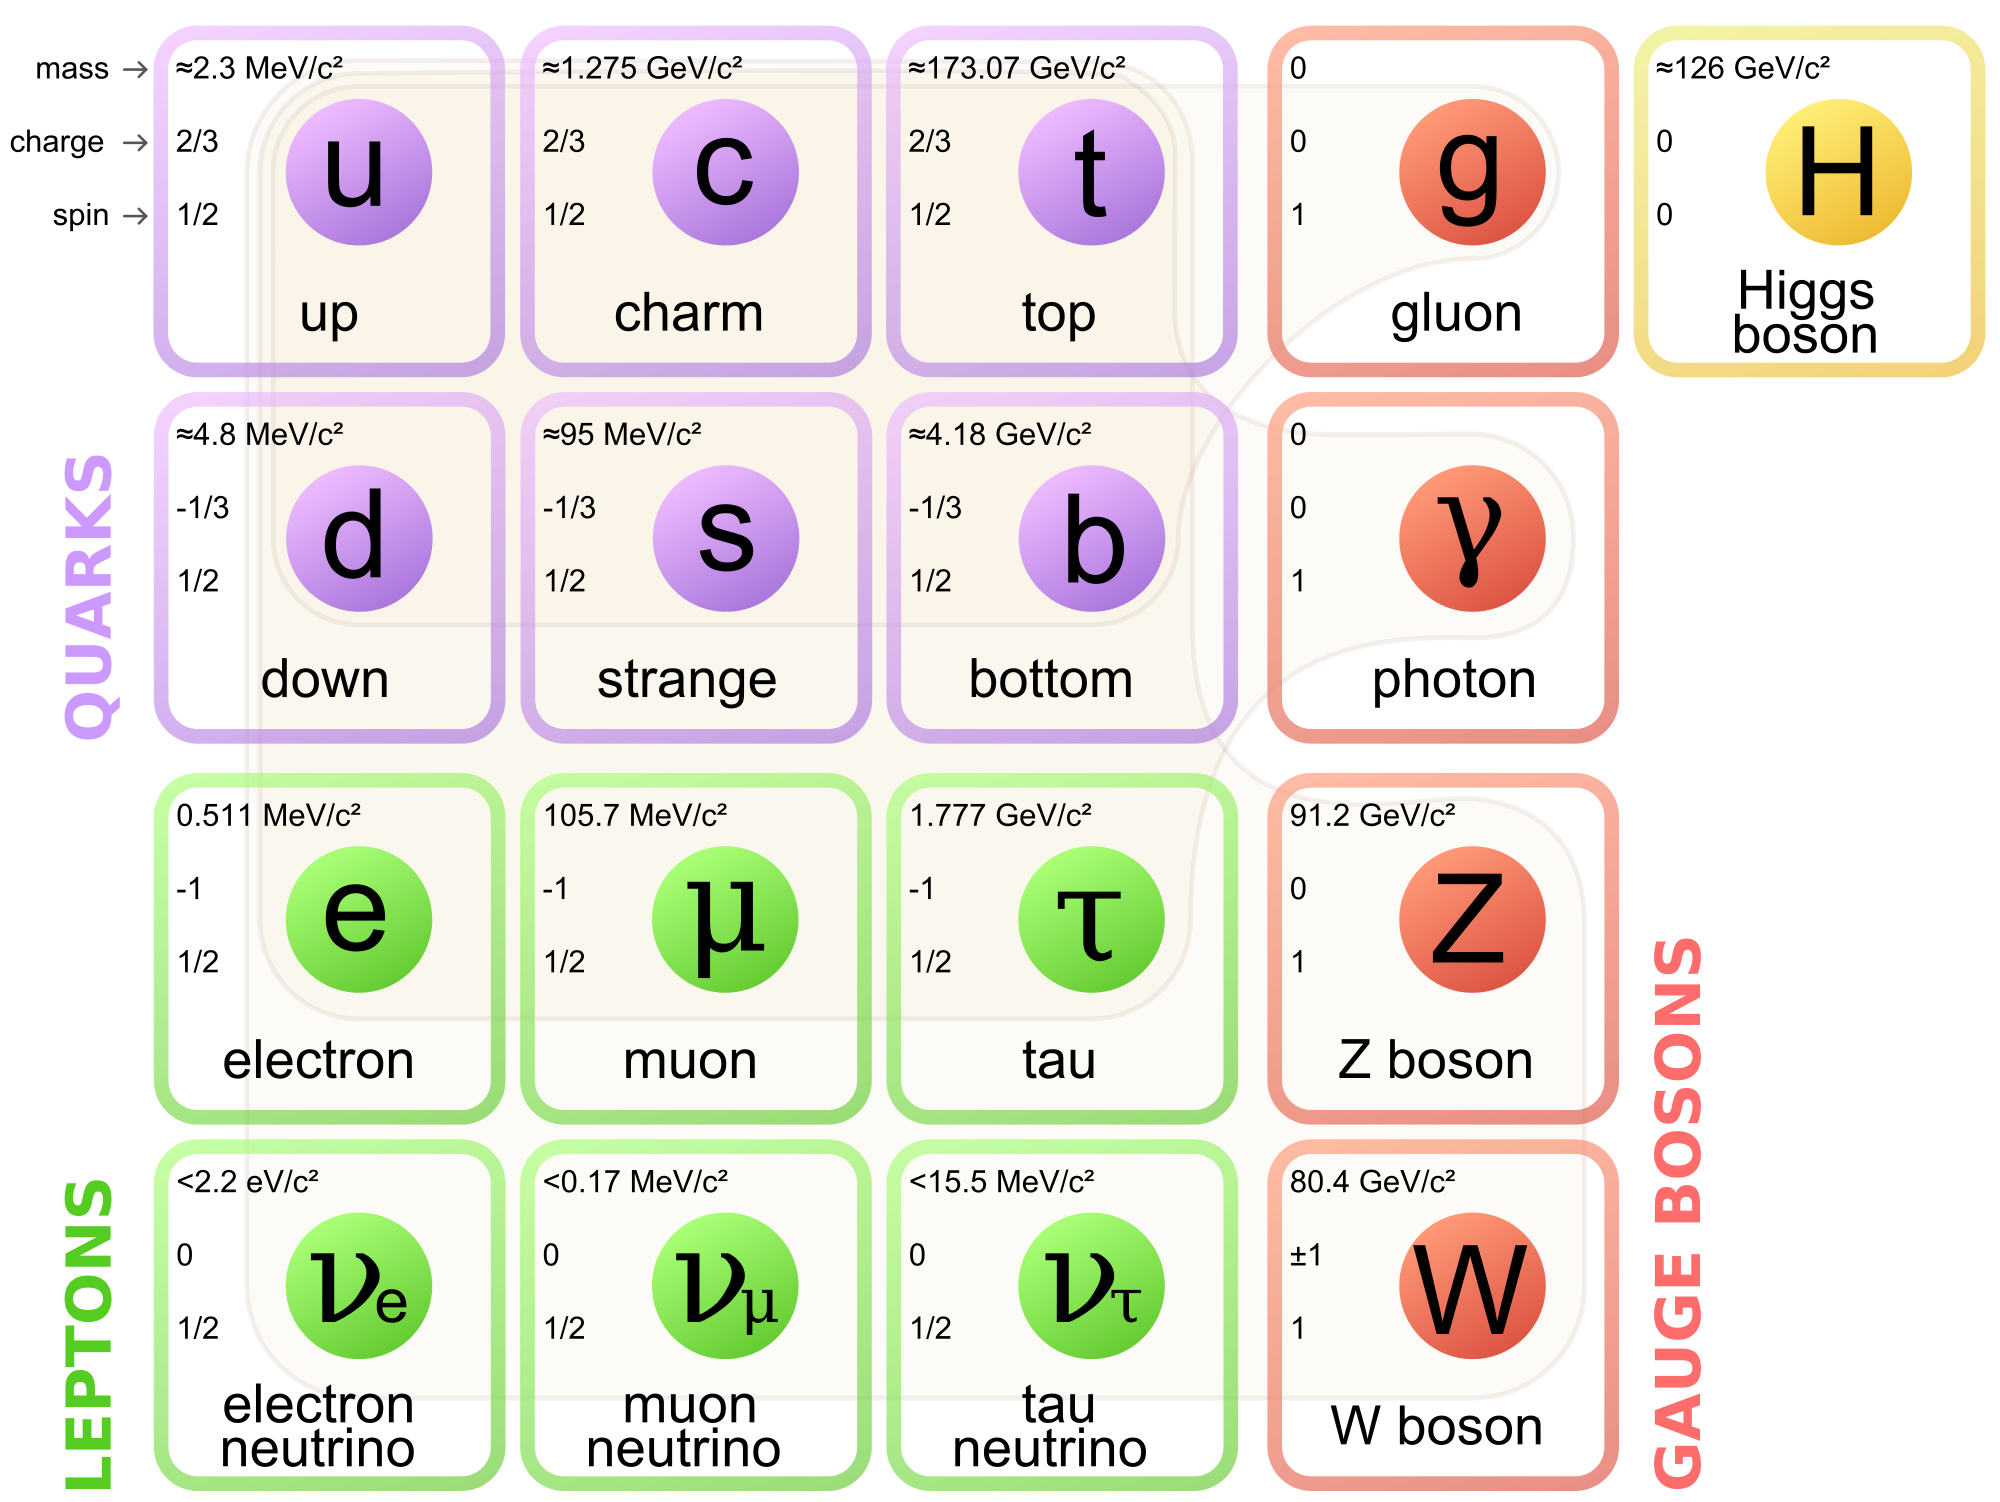
\includegraphics[width=0.9\textwidth]{IntroFigures/TheSM.png}
 \caption{The catalog of particles in the standard model.\label{fig:SMcartoon}}
\end{figure}

The dynamics and kinematics of the SM are controlled by the
Lagrangian density, which in conjunction with the particle content and
force carriers completes the theory. The lagrangian density is
presented below in compact formulation:
\begin{equation}
 \begin{aligned}
        \mathcal{L}_{\mathrm{SM}}& = -\frac{1}{4}B_{\mu\nu}B^{\mu\nu}
        -\frac{1}{4}W^{a}_{\mu\nu}W^{\mu\nu}_{a} - \frac{1}{4}G^{\alpha}_{\mu\nu}G^{\mu\nu}_{\alpha} 
        \qquad \text{gauge terms}\\
        &+\bar{\ell}_{\mathrm{L}}\tilde{\sigma}^{\mu}iD_{\mu}\ell_{\mathrm{L}}
        +\bar{e}_{\mathrm{R}}\sigma^{\mu}iD_{\mu}e_{\mathrm{L}} +
        \bar{\nu}_{\mathrm{R}}\sigma^{\mu}iD_{\mu}\nu_{\mathrm{L}} \qquad \text{lepton kinetic terms}\\
        &+\bar{q}_{\mathrm{L}}\tilde{\sigma}^{\mu}iD_{\mu}q_{\mathrm{L}}
        +\bar{u}_{\mathrm{R}}\sigma^{\mu}iD_{\mu}u_{\mathrm{L}} +
        \bar{d}_{\mathrm{R}}\sigma^{\mu}iD_{\mu}d_{\mathrm{L}} + \qquad \text{quark kinetic terms}\\
        &+\mathcal{L}_{\mathrm{Higgs}} +
        \mathcal{L}_{\mathrm{Yukawa}}\qquad \text{Higgs and Yukawa terms}
       \end{aligned}
\label{eq:theSMlagrangian}
\end{equation}

Where $\ell_{\mathrm{L}}=\begin{pmatrix}e_{\mathrm{L}}\\
  \nu_{\mathrm{L}}\end{pmatrix}$ is the lepton $\mathrm{SU(2)_{L}}$
doublet, $q_{\mathrm{L}}=\begin{pmatrix}u_{\mathrm{L}}\\
  d_{\mathrm{L}}\end{pmatrix}$ is the quark $\mathrm{SU(2)_{L}}$
doublet, $D_{\mu}$ is the corresponding covariant derivative, and
 $\sigma_{mu}$ is the identity and the pauli matrices ($\sigma_{mu} = {1,\sigma^{i}}$).
The $\mathcal{L}_{\mathrm{Higgs}}$ and $\mathcal{L}_{\mathrm{Yukawa}}$
are presented in sections~\ref{higgs} and~\ref{yukawa}, respectively.
Table~\ref{tab:SMGroup} presents the matter field representation in
the SM gauge group.

\begin{table}[htb]
\centering
\large
\begin{tabular}{cccc}
  \hline
  \hline
  field &  $\mathrm{SU(3)_{C}}$ &  $\mathrm{SU(2)_{L}}$ & $\mathrm{U(1)_{Y}}$\\
  \hline                                                        
  $q_{L}$ & $\mathbf{3}$ &  $\mathbf{2}$ & 1/6\\
  $\ell_{L}$ & $\mathbf{1}$ &  $\mathbf{2}$ & -1/2\\
  $u_{R}$ & $\mathbf{\bar{3}}$ &  $\mathbf{1}$ &-2/3\\
  $d_{R}$ & $\mathbf{\bar{3}}$ &  $\mathbf{1}$ &1/3\\
  $e_{R}$ & $\mathbf{1}$ &  $\mathbf{1}$ & 1\\
  $h$ & $\mathbf{1}$ &  $\mathbf{1}$ & 1/2\\
  \hline
  \hline
\end{tabular}
  \caption{\label{tab:SMGroup} Group representation of the matter
    fields in the SM.}
\end{table}
\section{The Higgs Boson and Electroweak Symmetry
  Breaking}\label{higgs}
Gauge theories prohibit -- in order to mantain the local symmetries --  explicit mass terms for the gauge bosons in the SM,
therefore all gauge bosons are massless. Since some of gauge boson in
the SM are massive ($W^{\pm}$,$Z$) there should be a mechanism by
which gauge boson acquire mass. The gauge boson masses in the SM are
realized by the \textit{spontaneous symmetry breaking} of the
$\mathrm{SU(2)_{L}}\times U(1)_{\mathrm{Y}}$ symmetry which induced by the nature of
the Higgs potential~\cite{HIGGES}. The best way to undertand this mechanism (the
Higgs mechanism) is to closely look at the lagrangian density:

\begin{equation}
\label{eq:higgsPotential}
\mathcal{L}_{\mathrm{Higgs}} =
(D^{\mu}\mathbf{\Phi})^{\dagger}(D^{\mu}\mathbf{\Phi}) +
V(\mathrm{\Phi});\hspace{1cm} V(\mathrm{\Phi}) = -\mu^{2}\Phi^{\dagger}\Phi +\lambda(\Phi^{\dagger}\Phi)^{2},
\end{equation}
where $D^{\mu}$ is the covariant derivative; $\Phi$ is a spin-0
complex field, and a $\mathrm{SU(2)_{L}}$ doublet with weak
hypercharge $\mathrm{Y} = 1/2$. The field is more easily represented
as a $\mathrm{SU(2)_{L}}$ doublet in the following fashion:
\begin{equation}
\label{eq:higgdoublet}
\Phi = \begin{pmatrix} \phi^{+}\\
  \phi^{0}\end{pmatrix}.
\end{equation}

When $\mu^{2} > 0$ the potential ($V(\Phi)$) has the commonly known
``Mexican hat'' shape, shown in Figure~\ref{fig:MexHat}, whith a minimum which does not preserve the
original $\mathrm{SU(2)_{L}}\times U(1)_{\mathrm{Y}}$
symmetry. Therefore the scalar field acquires a non-zero
\textit{vacuum expectation value (vev)}:
\begin{equation}
\label{eq:vev}
\langle \Phi \rangle \equiv \langle 0 | \Phi | 0\rangle = \frac{1}{\sqrt{2}}U(x) \begin{pmatrix} 0\\
  v\end{pmatrix}; \hspace{1cm}v = \sqrt{\frac{\mu^{2}}{\lambda}},
\end{equation}

\begin{figure}
 \centering
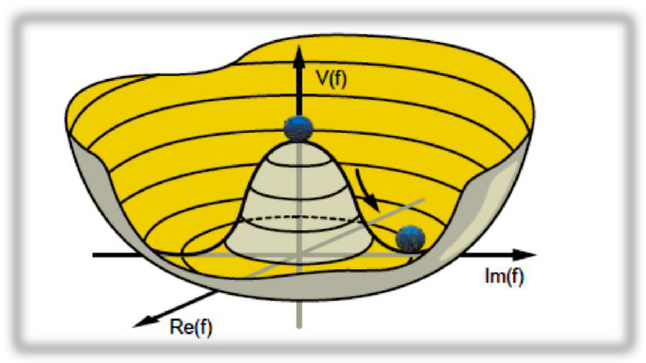
\includegraphics[width=0.9\textwidth]{IntroFigures/MexicanHat.png}
 \caption{The shape of the Higgs potential (``Mexican hat''). The
   degeneracy of the potential is observed along the azimuthal angle\label{fig:MexHat}}
\end{figure}

where $U(x)$ is a unitary transformation that transforms the field
into the degenerate solution. An important consequence is that the
\textit{vev} of field preserves a $U(1)$ symmetry from the original
$\mathrm{SU(2)_{L}}\times U(1)_{\mathrm{Y}}$ symmetry of the
lagrangian. Therefore the full electroweak symmetry of the SM
($\mathrm{SU(2)_{L}}\times U(1)_{\mathrm{Y}}$) is spontaneously broken
to $U(1)_{\mathrm{EM}}$.

This spontaneous breaking of the $\mathrm{SU(2)_{L}}\times
U(1)_{\mathrm{Y}}$ symmetry is responsible for the appearance of
masses to 3 of the four gauge bosons in the electroweak sector, this
is called: the Higgs mechanism. The masses become apparent when
replacing the \textit{vev} into the Higgs kinetic term in the
lagrangian:

\begin{equation}
\label{eq:HiggsMass}
(D^{\mu}\Phi)^{\dagger}(D^{\mu}\Phi) \rightarrow (\partial_{\mu}
-igA_{\mu}^{a}\tau^{a} - ig^{\prime}B_{\mu})^{\dagger}(\partial_{\mu}
-igA_{\mu}^{a}\tau^{a} - ig^{\prime}B_{\mu}) 
\end{equation}
\section{Fermion Masses}\label{yukawa}
\chapter{Supersymetry and Naturalness}
\chapter{Dark Matter and Weakly Interacting Particles}



%%%%%%%%%%%%%%%%
%%%%% New Part%%%%
%%%%%%%%%%%%%%%%
\part{The Large Hadron Collides and The Compact Muon Solenoid Experiment}
\chapter{The Large Hadron Collider}
\section{The Large Hadron Collider}
The CERN Large Hadron Collider (LHC) is a two-ring superconducting
accelerator and collider with 27 km of circumference, which is located
in the tunnel constructed for the CERN Large Electron-Positron
Collider (LEP). The tunnel lies between 45 m and 170 m below the
surface on an incliend plane (1.41\% slope) towards Lake L\`eman and
spans between the French and Swiss border close to Geneva. The layout
of the tunnel is such that contains 8 arc sections that spans most of
the circumference and 8 straight sections where the experimental halls
are located. 

The LHC is a particle-particle collider -- in its most common
configuration it collides protons -- with a designed center-of-mass
energy of 14\TeV. In order to achieve such high energies, the LHC uses
the existing CERN facilities to gradually increase the energy of the
protons. Everything starts with a bottle of compressed hydrogen gas,
then, hydrogen atoms are fed into the source chamber of the linear
accelerator, where an electric field strips off their
electrons. The resulting protons are then injected into the linear
accelaretor, Linac 2, which is the first step in the
accelerator chain and boosts the
protons energy up to 50\MeV. The accelated proton beam is then divided
into 4 (to increase its intensity) and enters the second stage of
acceleration, this occurs in the Proton Synchroton Booster (PSB),
where protons are now accelerated to 1.4\GeV. Subsequently, the proton beam is
recombined and sent to the Proton Synchrotron (PS), which increases
the energy to 25\GeV, followed by the Super Proton Synchrotron (SPS),
which brings the beam energy to 450\GeV.

Finally, the proton beam is transfered to the two beam pipes of the
LHC. The beams circulate in opposite directions. The LHC filling time
is 4 minutes and 20 seconds, but it takes around 20 minutes for the
protons to reach their maximum energy. Figure~\ref{fig:cernAcc} shows
the CERN accelerator complex just described.
\begin{figure}
 \centering
 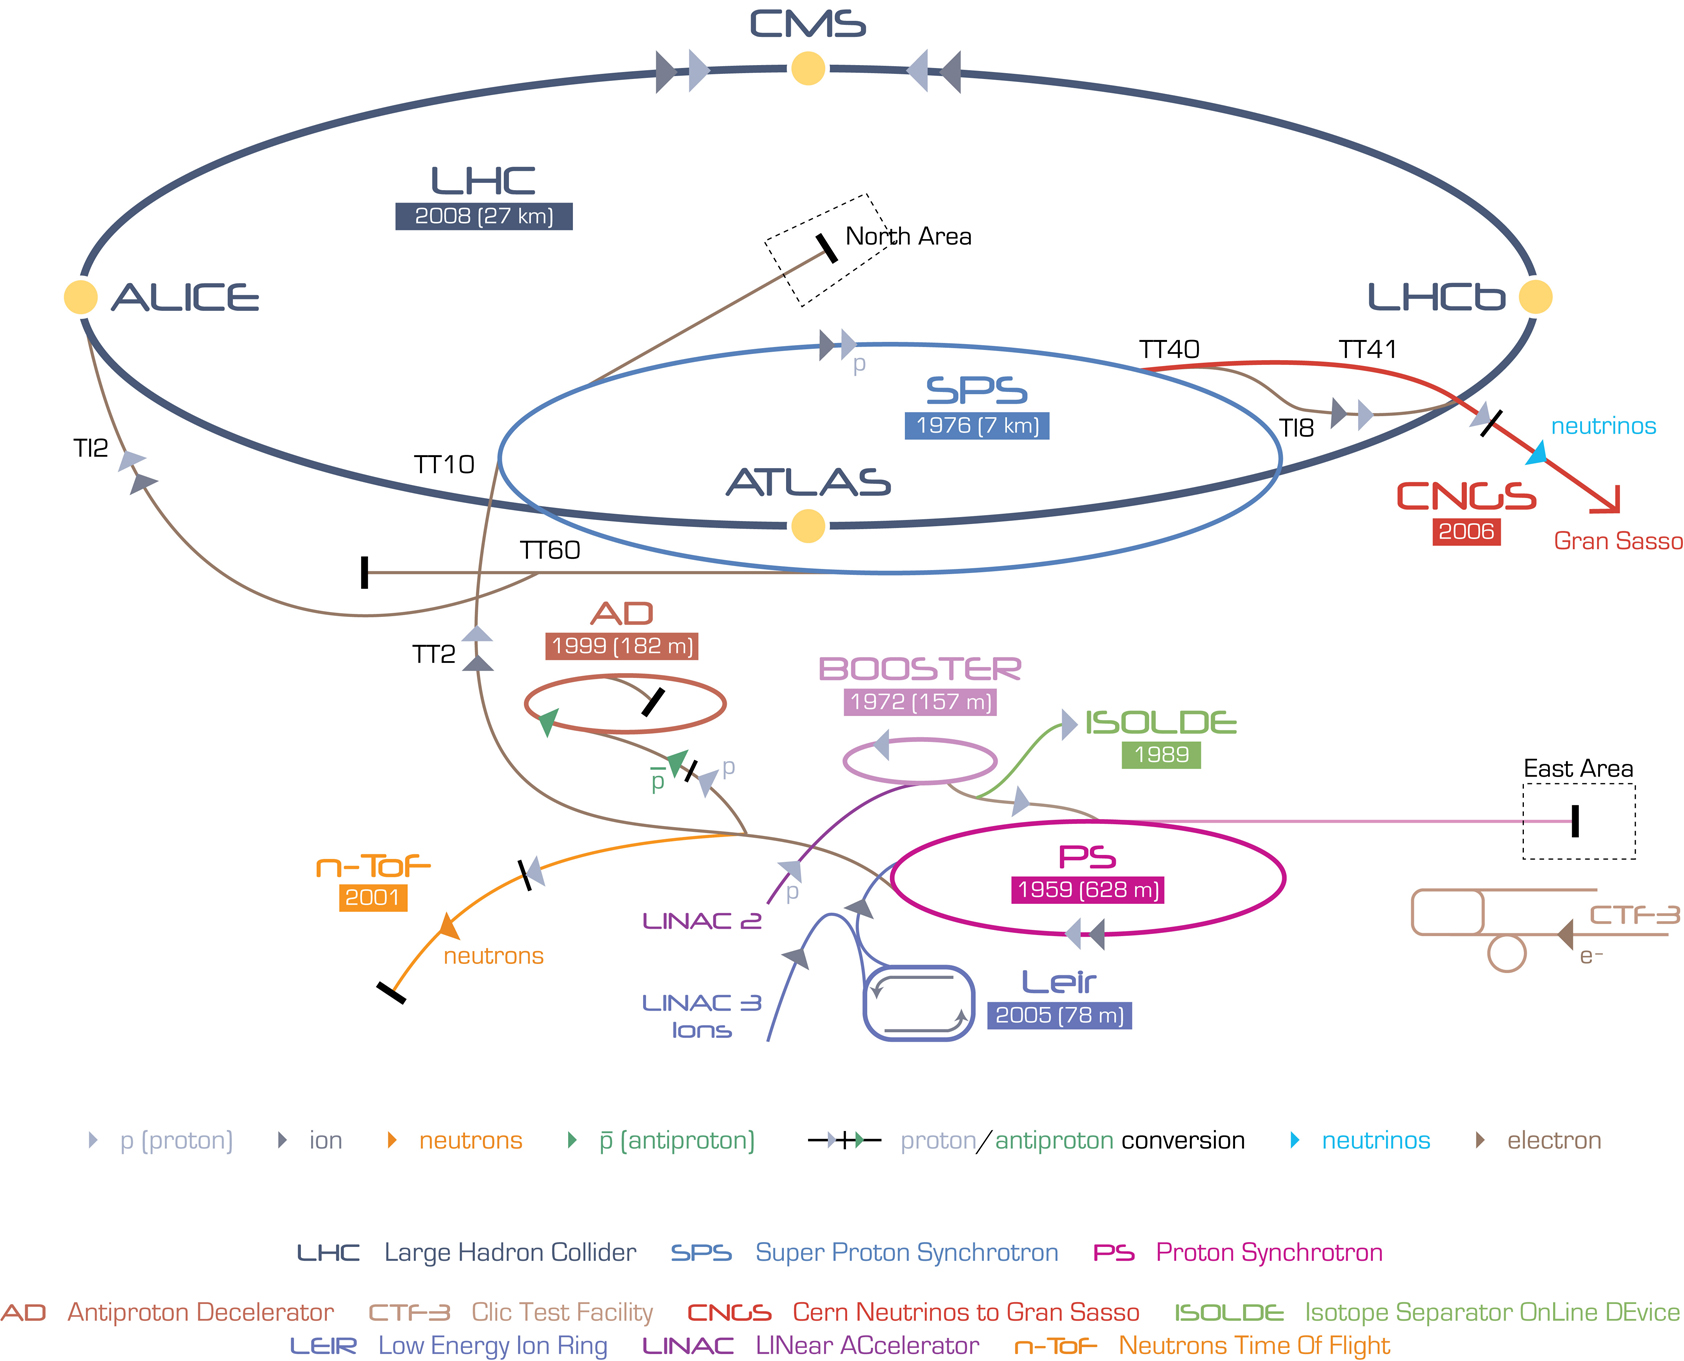
\includegraphics[width=0.9\textwidth]{LHC_fig/Cern-Accelerator-Complex.jpg}
 \caption{The CERN accelerator complex.\label{fig:cernAcc} }
\end{figure}
At this point, the two beams are brought to collide at the four interaction points (IP) in the straight
sections where the LHC's experiments are located. There are two main
purpose experiments located in diametrical opposite locations, the
ATLAS experiment is located at point 1 and the CMS experiment is
located at point 1. There are also two specialized experiments; the
LHCb experiment, which studies B-hadron physics, and the ALICE
experiment, which specializes in studying heavy ion collisions (another type of
collision possible at the LHC). Figure~\ref{fig:LHC} shows an
squematic layout of the LHC.
\begin{figure}
 \centering
 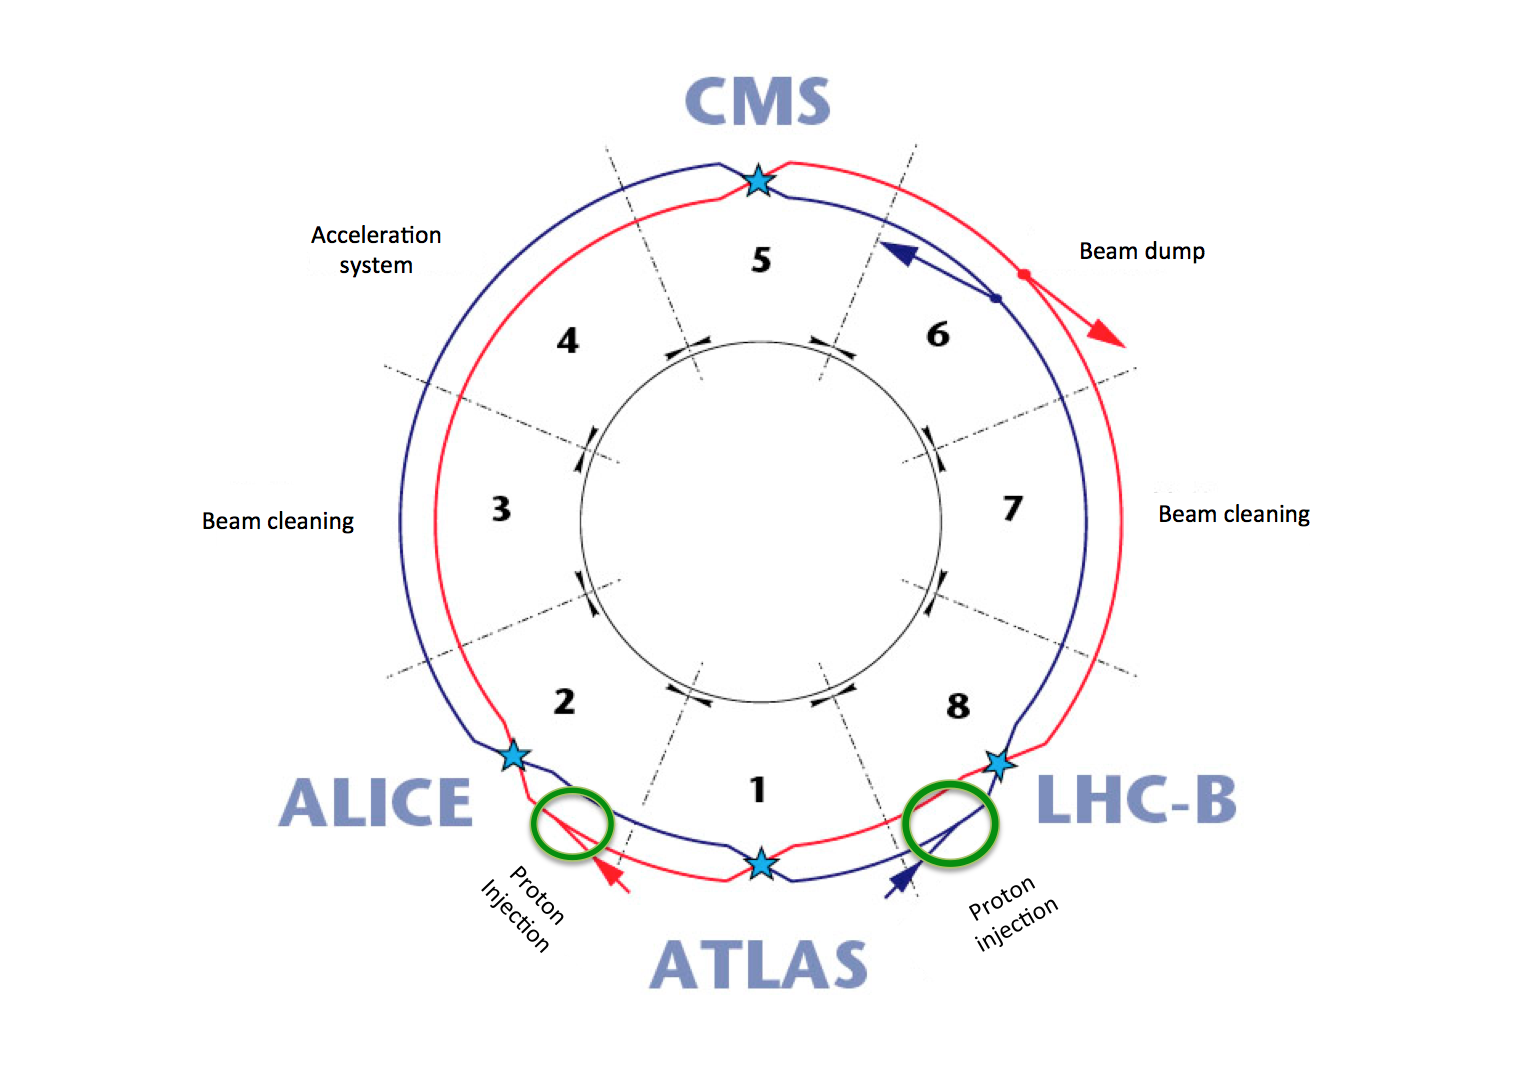
\includegraphics[width=0.9\textwidth]{LHC_fig/LHC_layout.png}
 \caption{The CERN Large Hadron Collider schematic layout.\label{fig:LHC} }
\end{figure}
Due to the small diameter of the tunnel in the arcs
(3.7~m), which complicates the installation of two separate proton
rings, the LHC uses a twin-bore magnet design, proposed in 1971 by
John Blewett at the Brookhaven National Laboratory
(BNL)~\cite{JBlewett} as a cost-saving alternative. 

Since the usage of superconducting magnets a the Intersecting  Storage
Rings at CERN, particle colliders have used them as the default
technology for their operation. However, the main difference is that the LHC's
superconducting magnets operate at a tempareture lower (below 2~K) than the
standard superconducting magnets in other particle colliders
(4-5~K). The LHC ring accomodates 1,232 NbTi main dipole magnets,
cooled down to 1.9 K by using superfluid helium; they operate at fields
above 8~T. The twin-bore desing allow for a common nonmagnetic collar
and iron yoke, as well as common cryogenic system. The core of the
dipole magnet system is enclosed by a cylindrical alloyed low-carbon steel vacuum vessel with an outer diameter of 914\mm and a wall
thickness of 12\mm. Figures~\ref{fig:magnet1} and~\ref{fig:magnet2} show a cross sectional
view and a 3-dimensional visualization of the main dipole magnet
system, respectively.
\begin{figure}
 \centering
 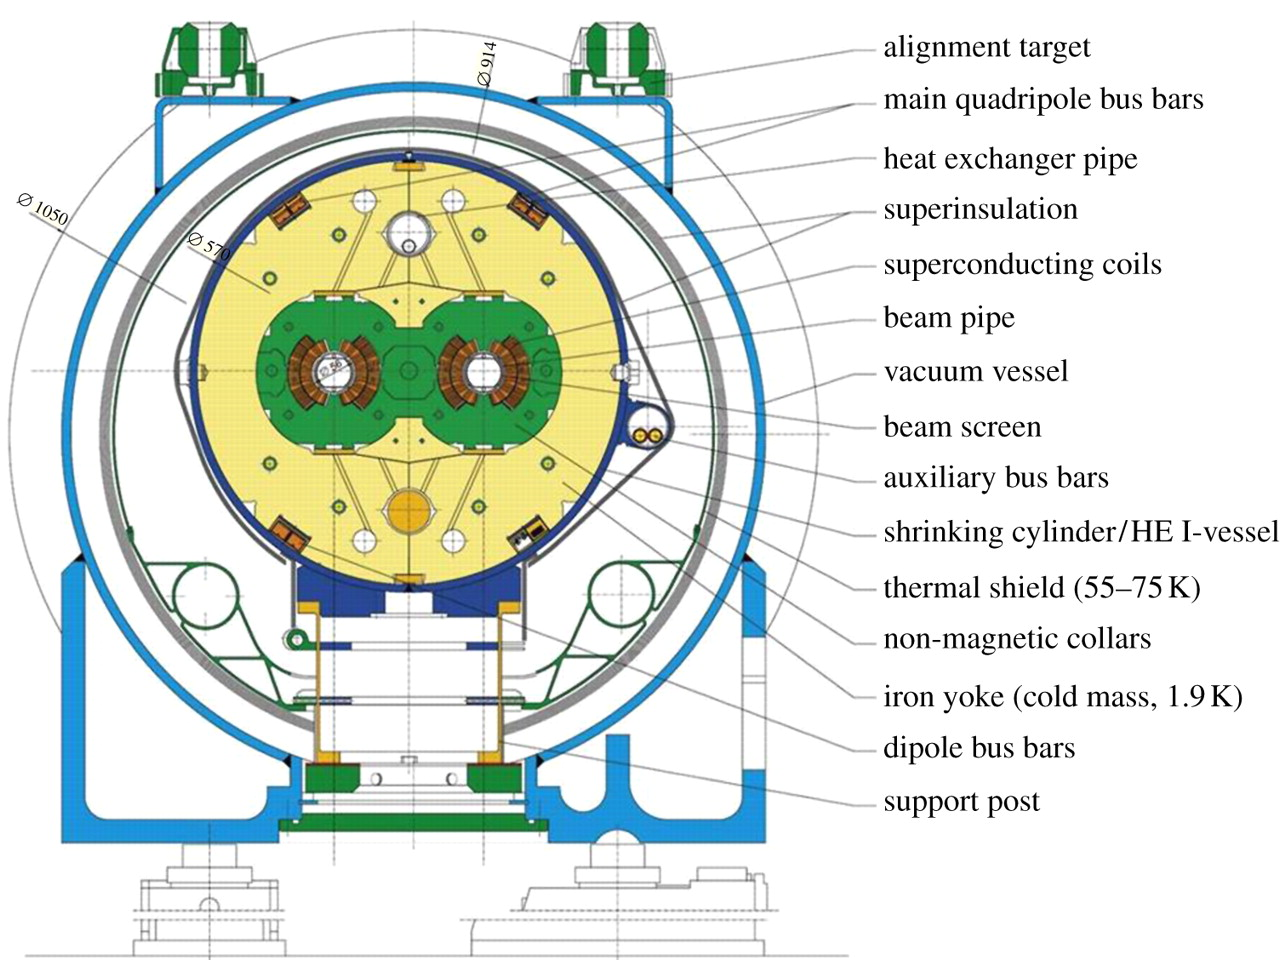
\includegraphics[width=0.9\textwidth]{LHC_fig/ColdMassMagnet.jpg}
 \caption{An schematic cross sectional view of the LHC dipole magnet.\label{fig:magnet1} }
\end{figure}
\begin{figure}
 \centering
 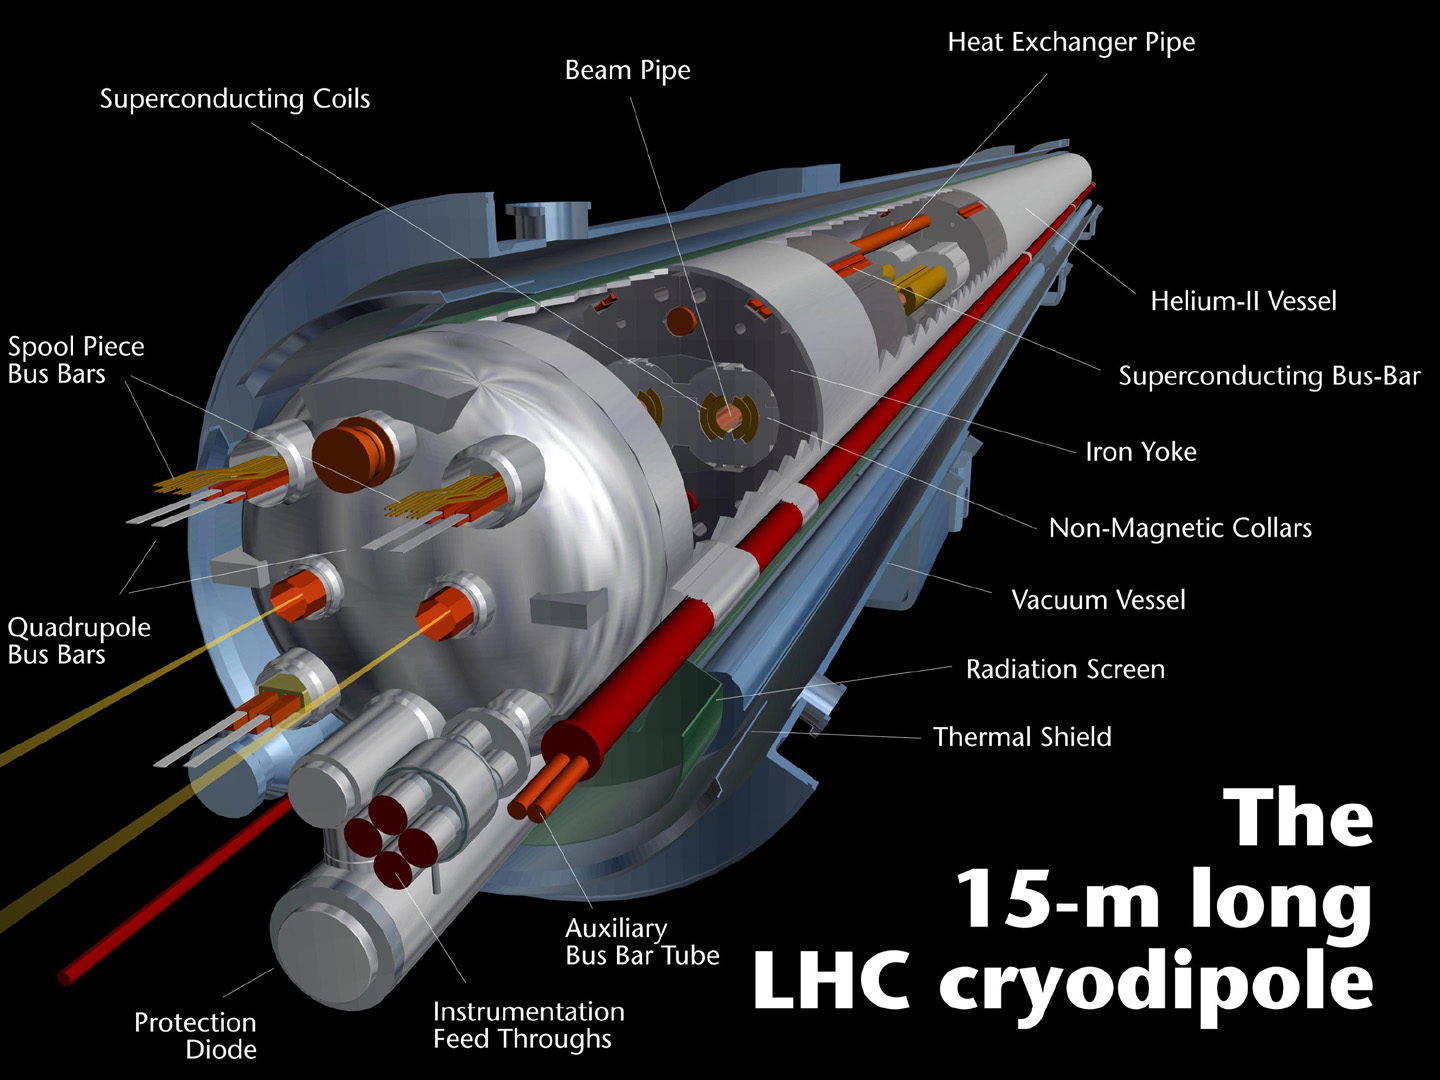
\includegraphics[width=0.9\textwidth]{LHC_fig/cryodipole.jpg}
 \caption{An 3D visualization of a LHC dipole magnet.\label{fig:magnet2} }
\end{figure}

The goal of the LHC program is to reveal the nature of new
physics. The high-energy collision (14\TeV) are a key ingredient to probe new
physics, since new physics could just be present at that energy
scale. However, it is by no means the only ingredient; new physics
will likely have smaller cross sections than that of the known SM
processes and therefore a large number of proton-proton collision is
needed. The number of events for a particular physics process $N_{exp}$
generated in the LHC is the product of the experimental cross section $\sigma_{exp}$
and the integrated luminosity, i.e.
\begin{equation}
N_{exp} = \sigma_{exp}\int\mathcal{L}(t)dt.
\end{equation}
Where $\mathcal{L}(t)$ is the instantaneous luminosity, which depends
on the LHC beam parameters and can be written as\cite{LHCbeamParam}:
\begin{equation}
\mathcal{L}(t) = \frac{N^{2}_{b}n_{b}f_{rev}\gamma_{r}}{4\pi\epsilon_{n}\beta^{*}},
\end{equation}
where $N_{b}$ is the number of particles per bunch, $n_{b}$ is the
number of bunches per beam, $f_{rev}$ is the revolution frequency,
$\gamma_{r}$ is the relativistic factor, $\epsilon_{n}$ is the
normalized transverse beam emittance, $\beta^{*}$ is the transverse
size of the beam at the IP, and $F$ is the geometric luminosity
reduction factor due to the crossing angle at the IP:
\begin{equation}
F=\left(1+\left(\frac{\theta_{c}\sigma_{z}}{2\sigma^{*}}\right)\right)^{-1/2}
\end{equation}
In the last expression, $\theta_{c}$ is the full crossing angle at the
IP, $\sigma_{z}$ is the rms bunch length, and $\sigma^{*}$ is the
transverse rms beam size at the IP. The designed peak luminosity to be
deliverd the ATLAS and CMS is $\mathcal{L}(t) = 10^{34}$~cm$^-2$~s$^{-1}$.  
Figure~\ref{fig:lumi} shows the integrated luminosity
received by the CMS experiment from 2007 to 2016. 
\begin{figure}
 \centering
 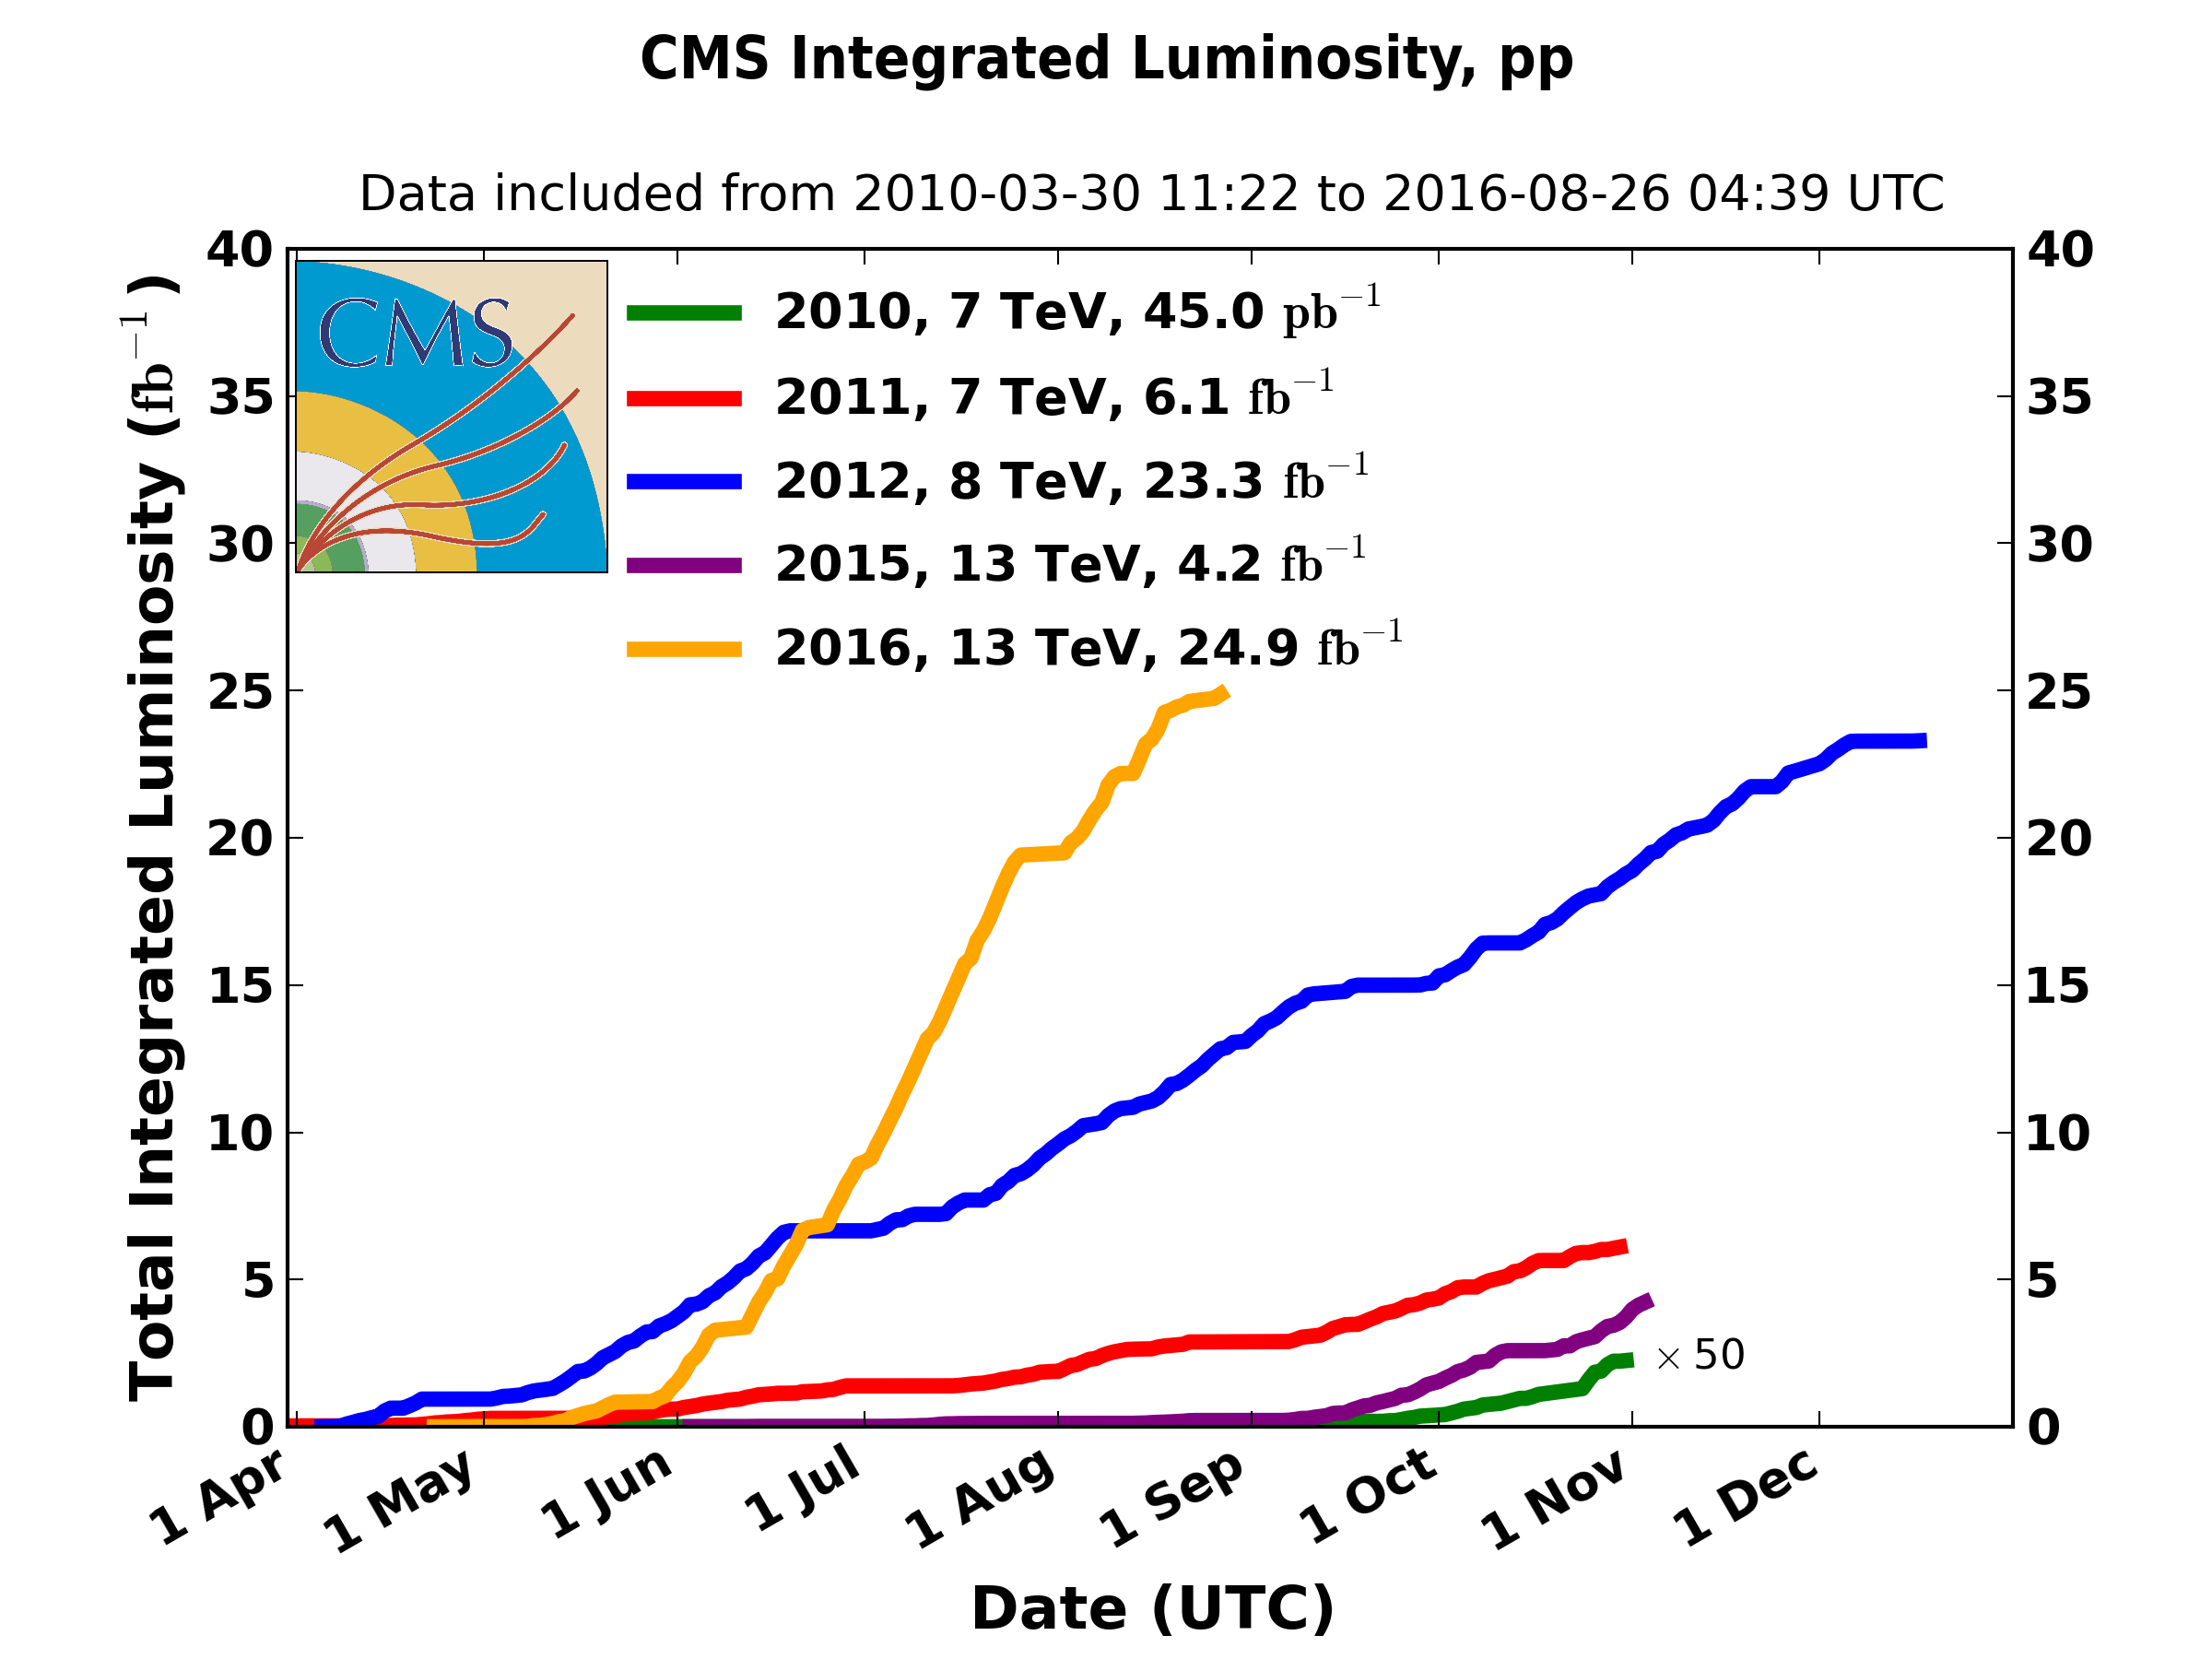
\includegraphics[width=0.9\textwidth]{LHC_fig/int_lumi_cumulative_pp_2.png}
 \caption{Intregated luminosity received by the CMS experiment during the LHC operation.\label{fig:lumi} }
\end{figure}

\chapter{The Compact Muon Solenoid Experiment}
\section{Detector System}
The Compact Muon Solenoid (CMS) detector operates at the LHC at CERN. It was designed to operate in proton-proton (and lead-lead)
collisions at a center-of-mass energy of 14\TeV (5.5\TeV) and at
luminosities up to 10$^{34}$cm$^{-2}$s$^{-1}$
(10$^{27}$cm$^{-2}$s$^{-1}$). The CMS has cilindrical geometry and
its dimensions are a length of 21.5 m, a diameter of 14.6, and a total
weight of 12,500 tons. At the heart of the CMS detector system
lies a 4\unit{T} magnetic field produced by a large-bore superconducting
solenoid which encloses a silicon -- pixel and strips -- tracker, a homogeneous
lead-tungstate crystal electromagnetic calorimeter, and a brass-scintillator
sampling hadron calorimeter. Outside the superconducting solenoid lies
an iron yoke for magnetic flux-return instrumented with four stations
for muon detection. Forward sampling calorimeters extend the rapidity
coverage up to $\eta < 5$ and thus ensure good
hemiticity. Figure~\ref{fig:cmsDetector} shows an schematic representation
of the CMS detector and Figure~\ref{fig:cmsSlice} shows a cartoon
with a cross-sectional-slice view of the CMS detector along with
different particle detections.
\begin{figure}
 \centering
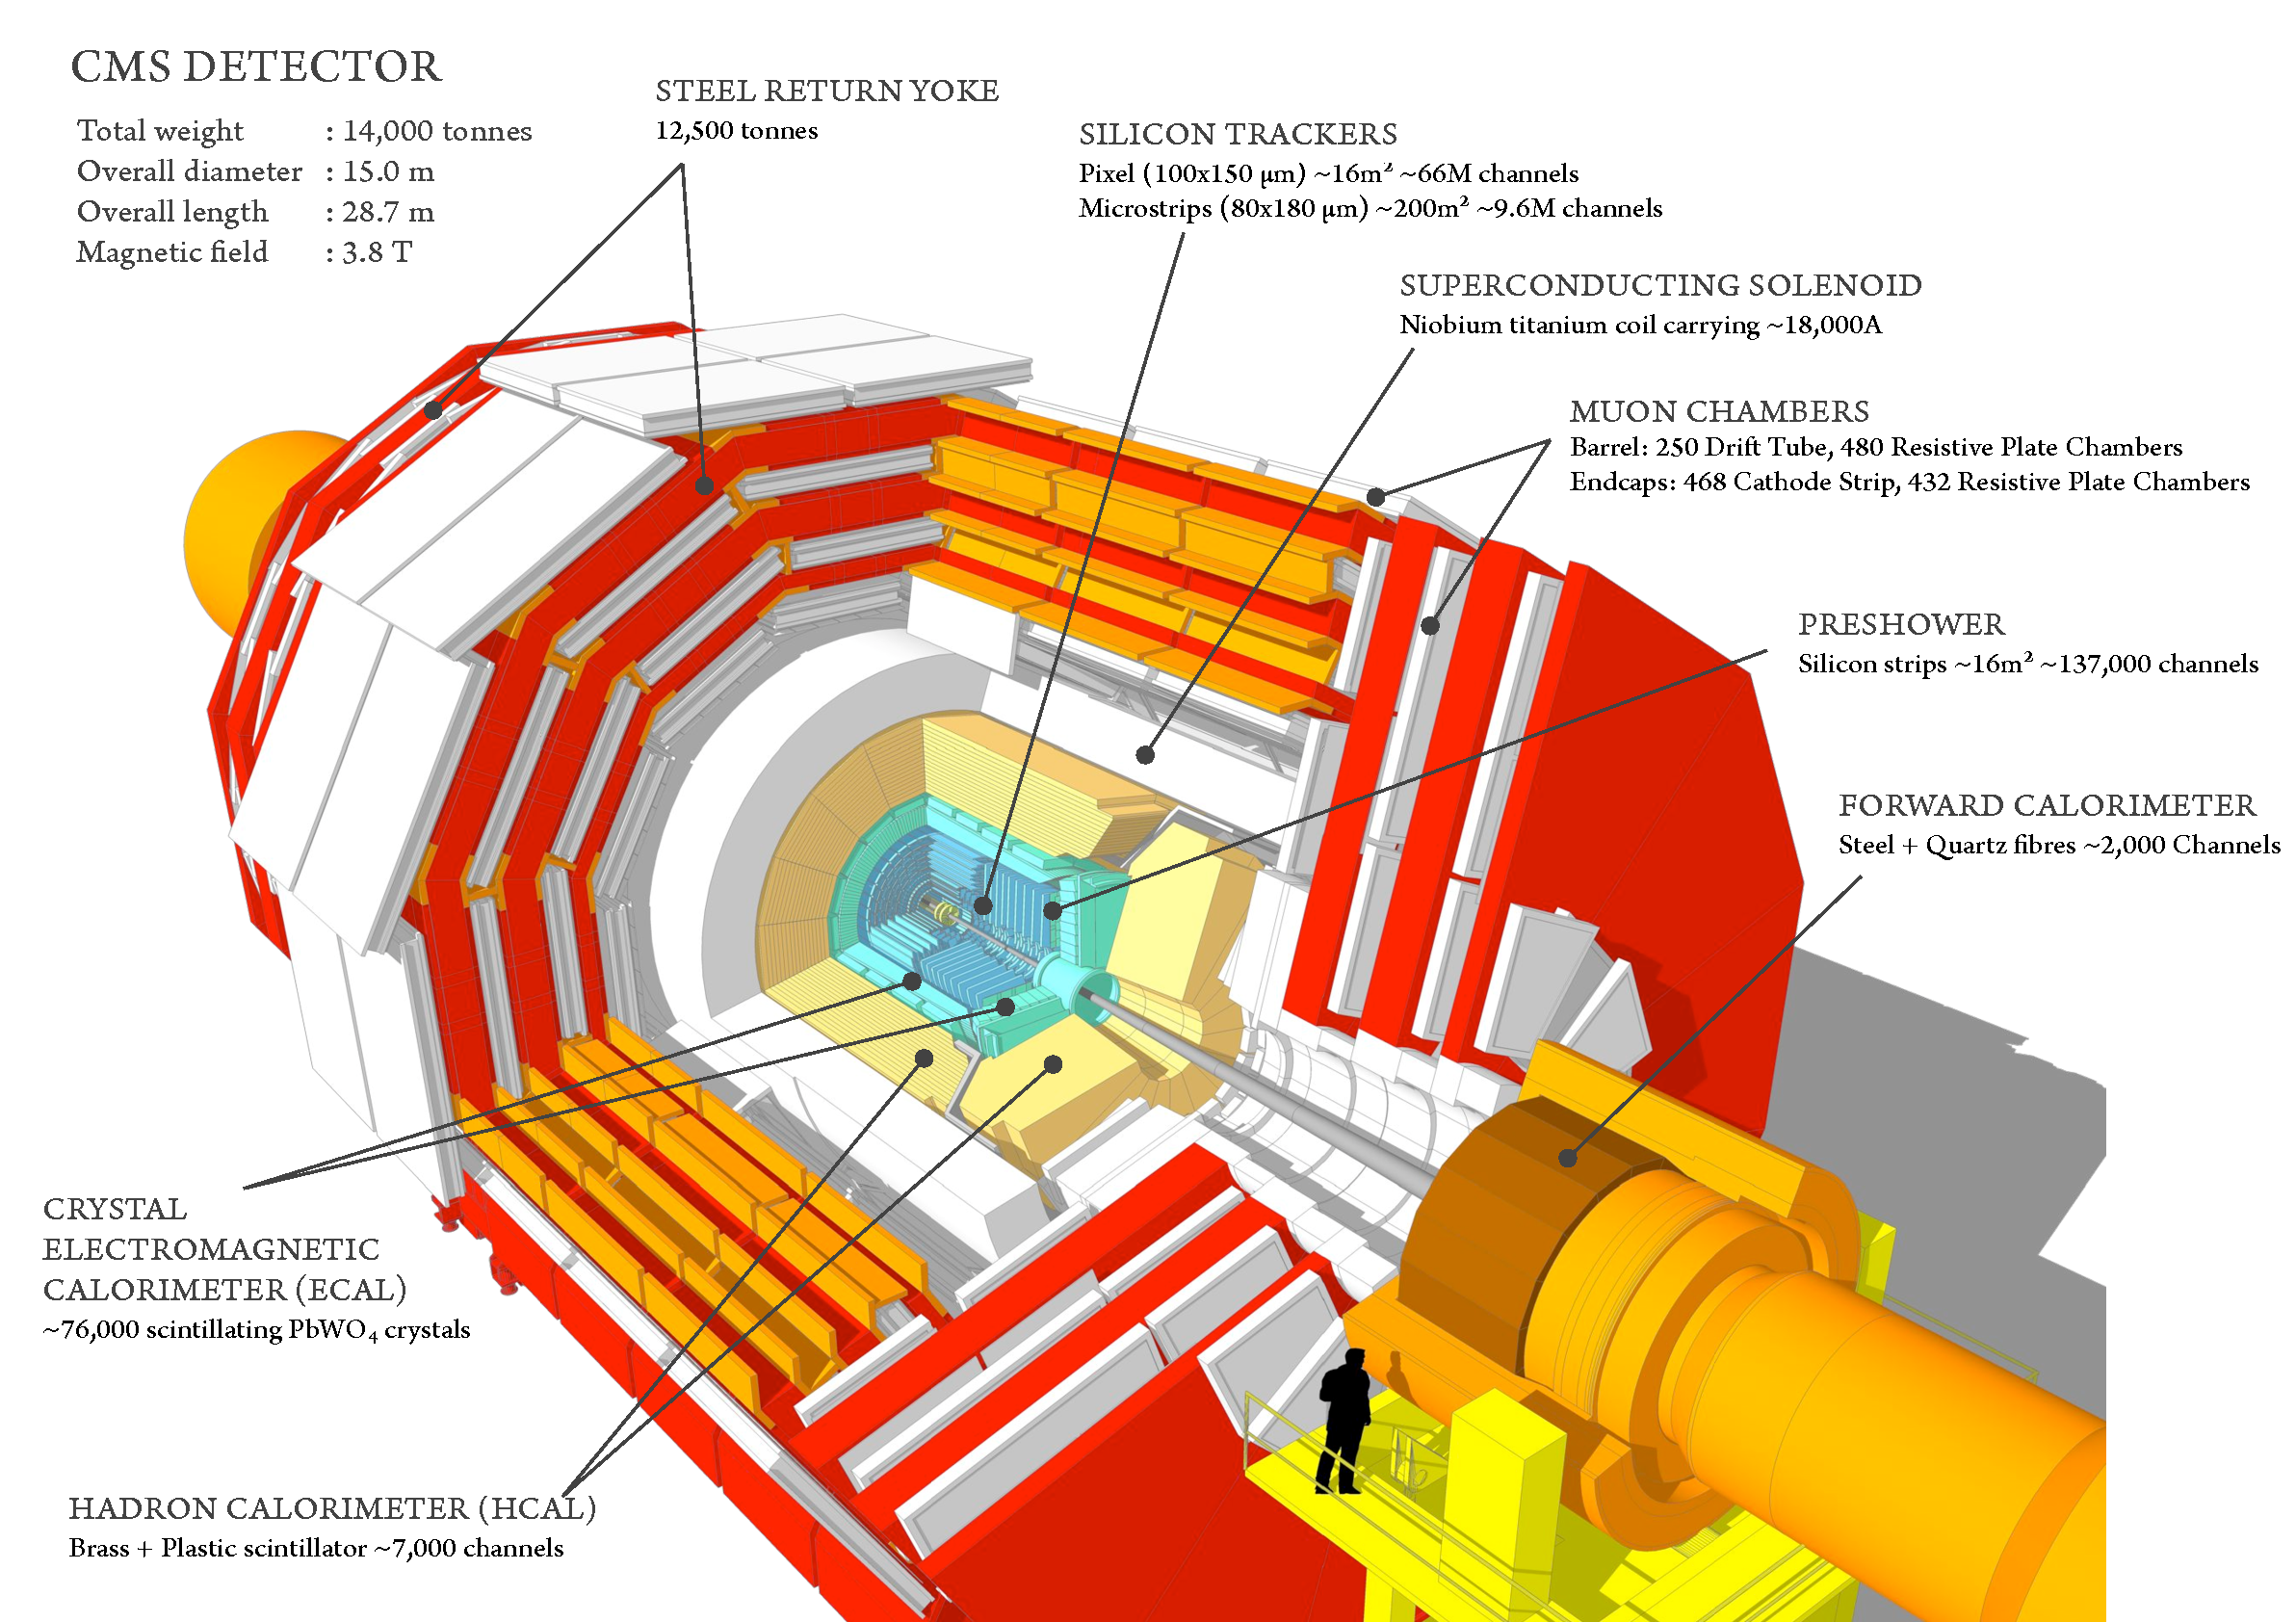
\includegraphics[width=0.99\textwidth]{CMS_DetectorFigures/cms_detector.png}
 \caption{A perspective view of the CMS detector.\label{fig:cmsDetector}}
\end{figure}
\begin{figure}
 \centering
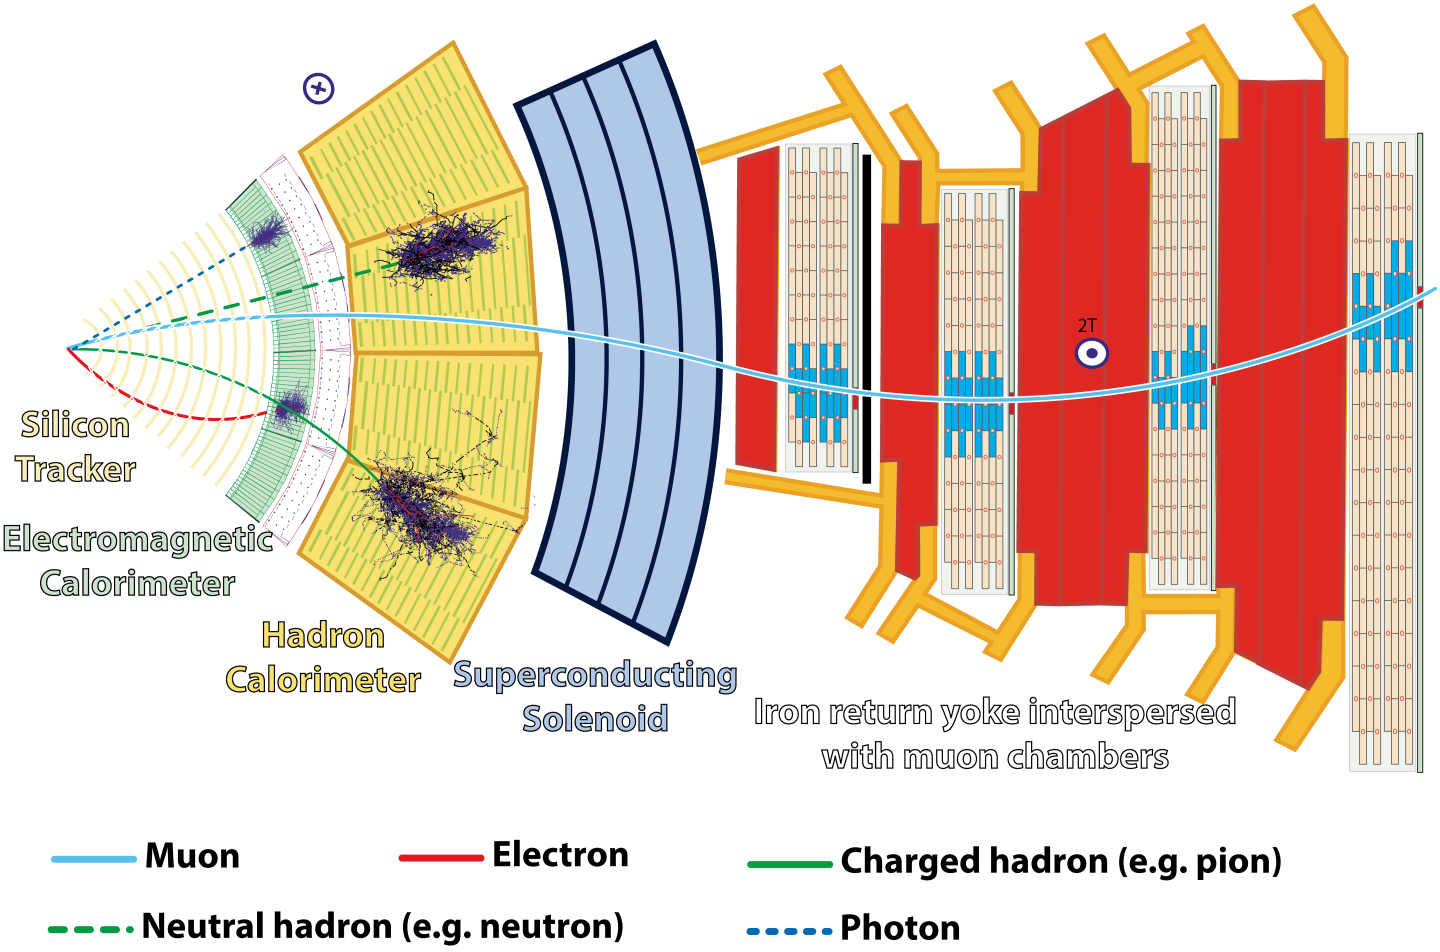
\includegraphics[width=0.99\textwidth]{CMS_DetectorFigures/CMSslice.png}
 \caption{A cross-sectional-slice view of the CMS detector. The
   different components of the detector are clearly labeled and
   different particle detections are depicted.\label{fig:cmsSlice}}
\end{figure}

This chapter presents an introduction to the CMS detector systems and
reconstruction algorithms. It is by no means a complete picture of the
CMS detector and its mostly based on Ref.~\cite{Chatrchyan:2008zzk}.
\section{The Tracker System}
The tracker is the innermost system of the CMS detector.
It was designed to measure efficiently and precisely the trajectories
of charged particles coming from the interaction points, as well as to
provide a precise reconstruction of the secondary vertices at each
bunch crossing. When running at the LHC designed conditions, every
buch crossing, i.e 25 ns, the number of proton-proton collision will
be about 20 and they will produce an average number of particles of about
1000. These conditions and the above requirements implied a highly granular and fast
response design. That being said, this design due to its high power
consumption requires an efficient cooling system which in turn is in
conflict with the goal of minimizing the material budget and thus
reduce unwanted interactions. In addition, the harsh radiation
environment that will deteriorate the detector performance posed
further challenges in its construction. Therefore, the system --
silicon sensors, readout, mechanical structures, granularity, etc --
was designed to operate for 10 year and satisfying the considerations
listed above. The CMS tracker is composed of three layers of pixels
detectors up to a radius of 10.2 cm, a 10-layer silicon strip tracker
up to a radious of 1.1 m, two endcap disks at each side of the barrel pixel detectors, 3
endcap disks at each side of the inner region of the strips (up to a
radius of 55 cm), and finally 9 disks covering the $|z|$ > 120 cm
regions starting a radious of 55 cm. More details about the tracker
layout will be given below and are summarized in
Figure~\ref{fig:trackerlayout}. The tracker covers up to
pseudorapidities of $|eta| < 2.5$ with a about 200 m$^2$ of active
silicon area implemented. The material budget of the CMS tracker is
shown in Figure~\ref{fig:materialBudget}. As it can be seen the most
heavily implemented pseudorapidity is found to be at $|\eta|\approx$ 1.4.
\begin{figure}
 \centering
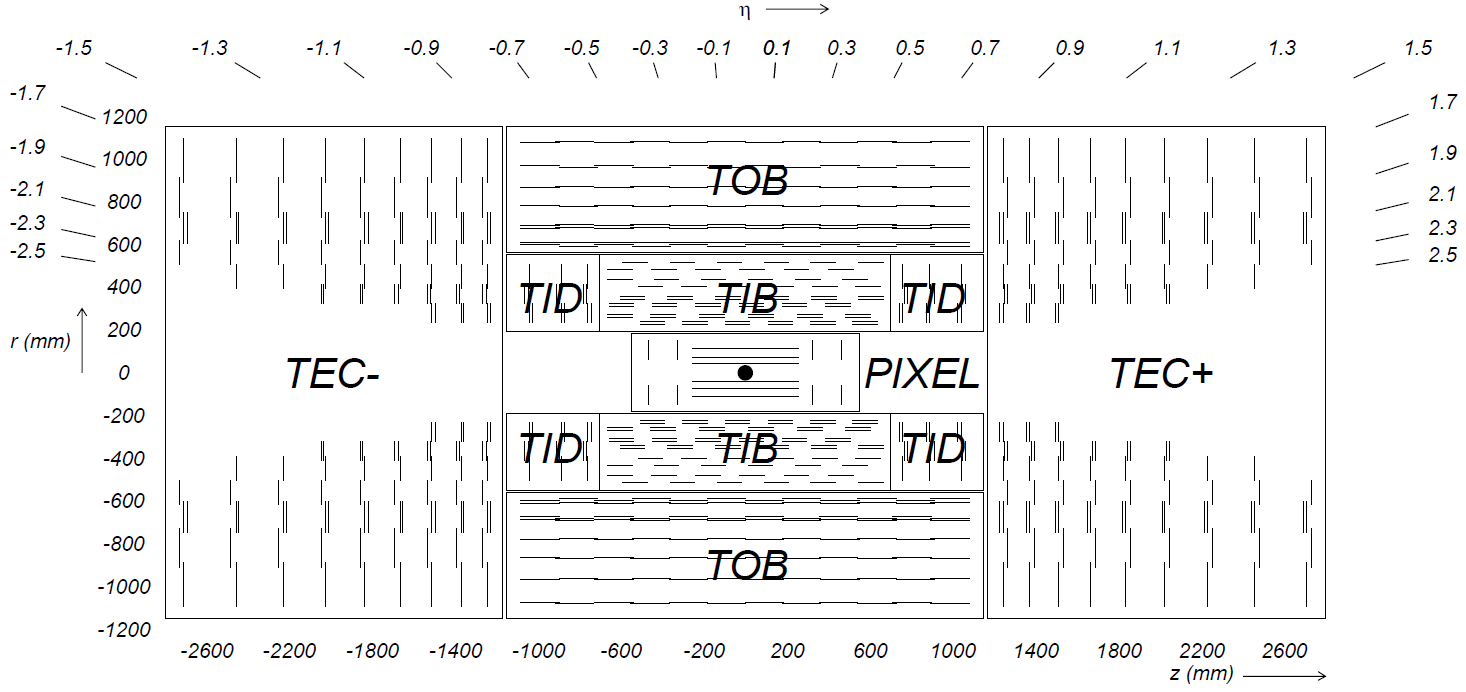
\includegraphics[width=0.99\textwidth]{CMS_DetectorFigures/TrackerLayout.png}
 \caption{A cross-sectional view of the silicon tracker layout. The
   different subsytems are clearly labeled.\label{fig:trackerlayout}}
\end{figure}
\begin{figure}
 \centering
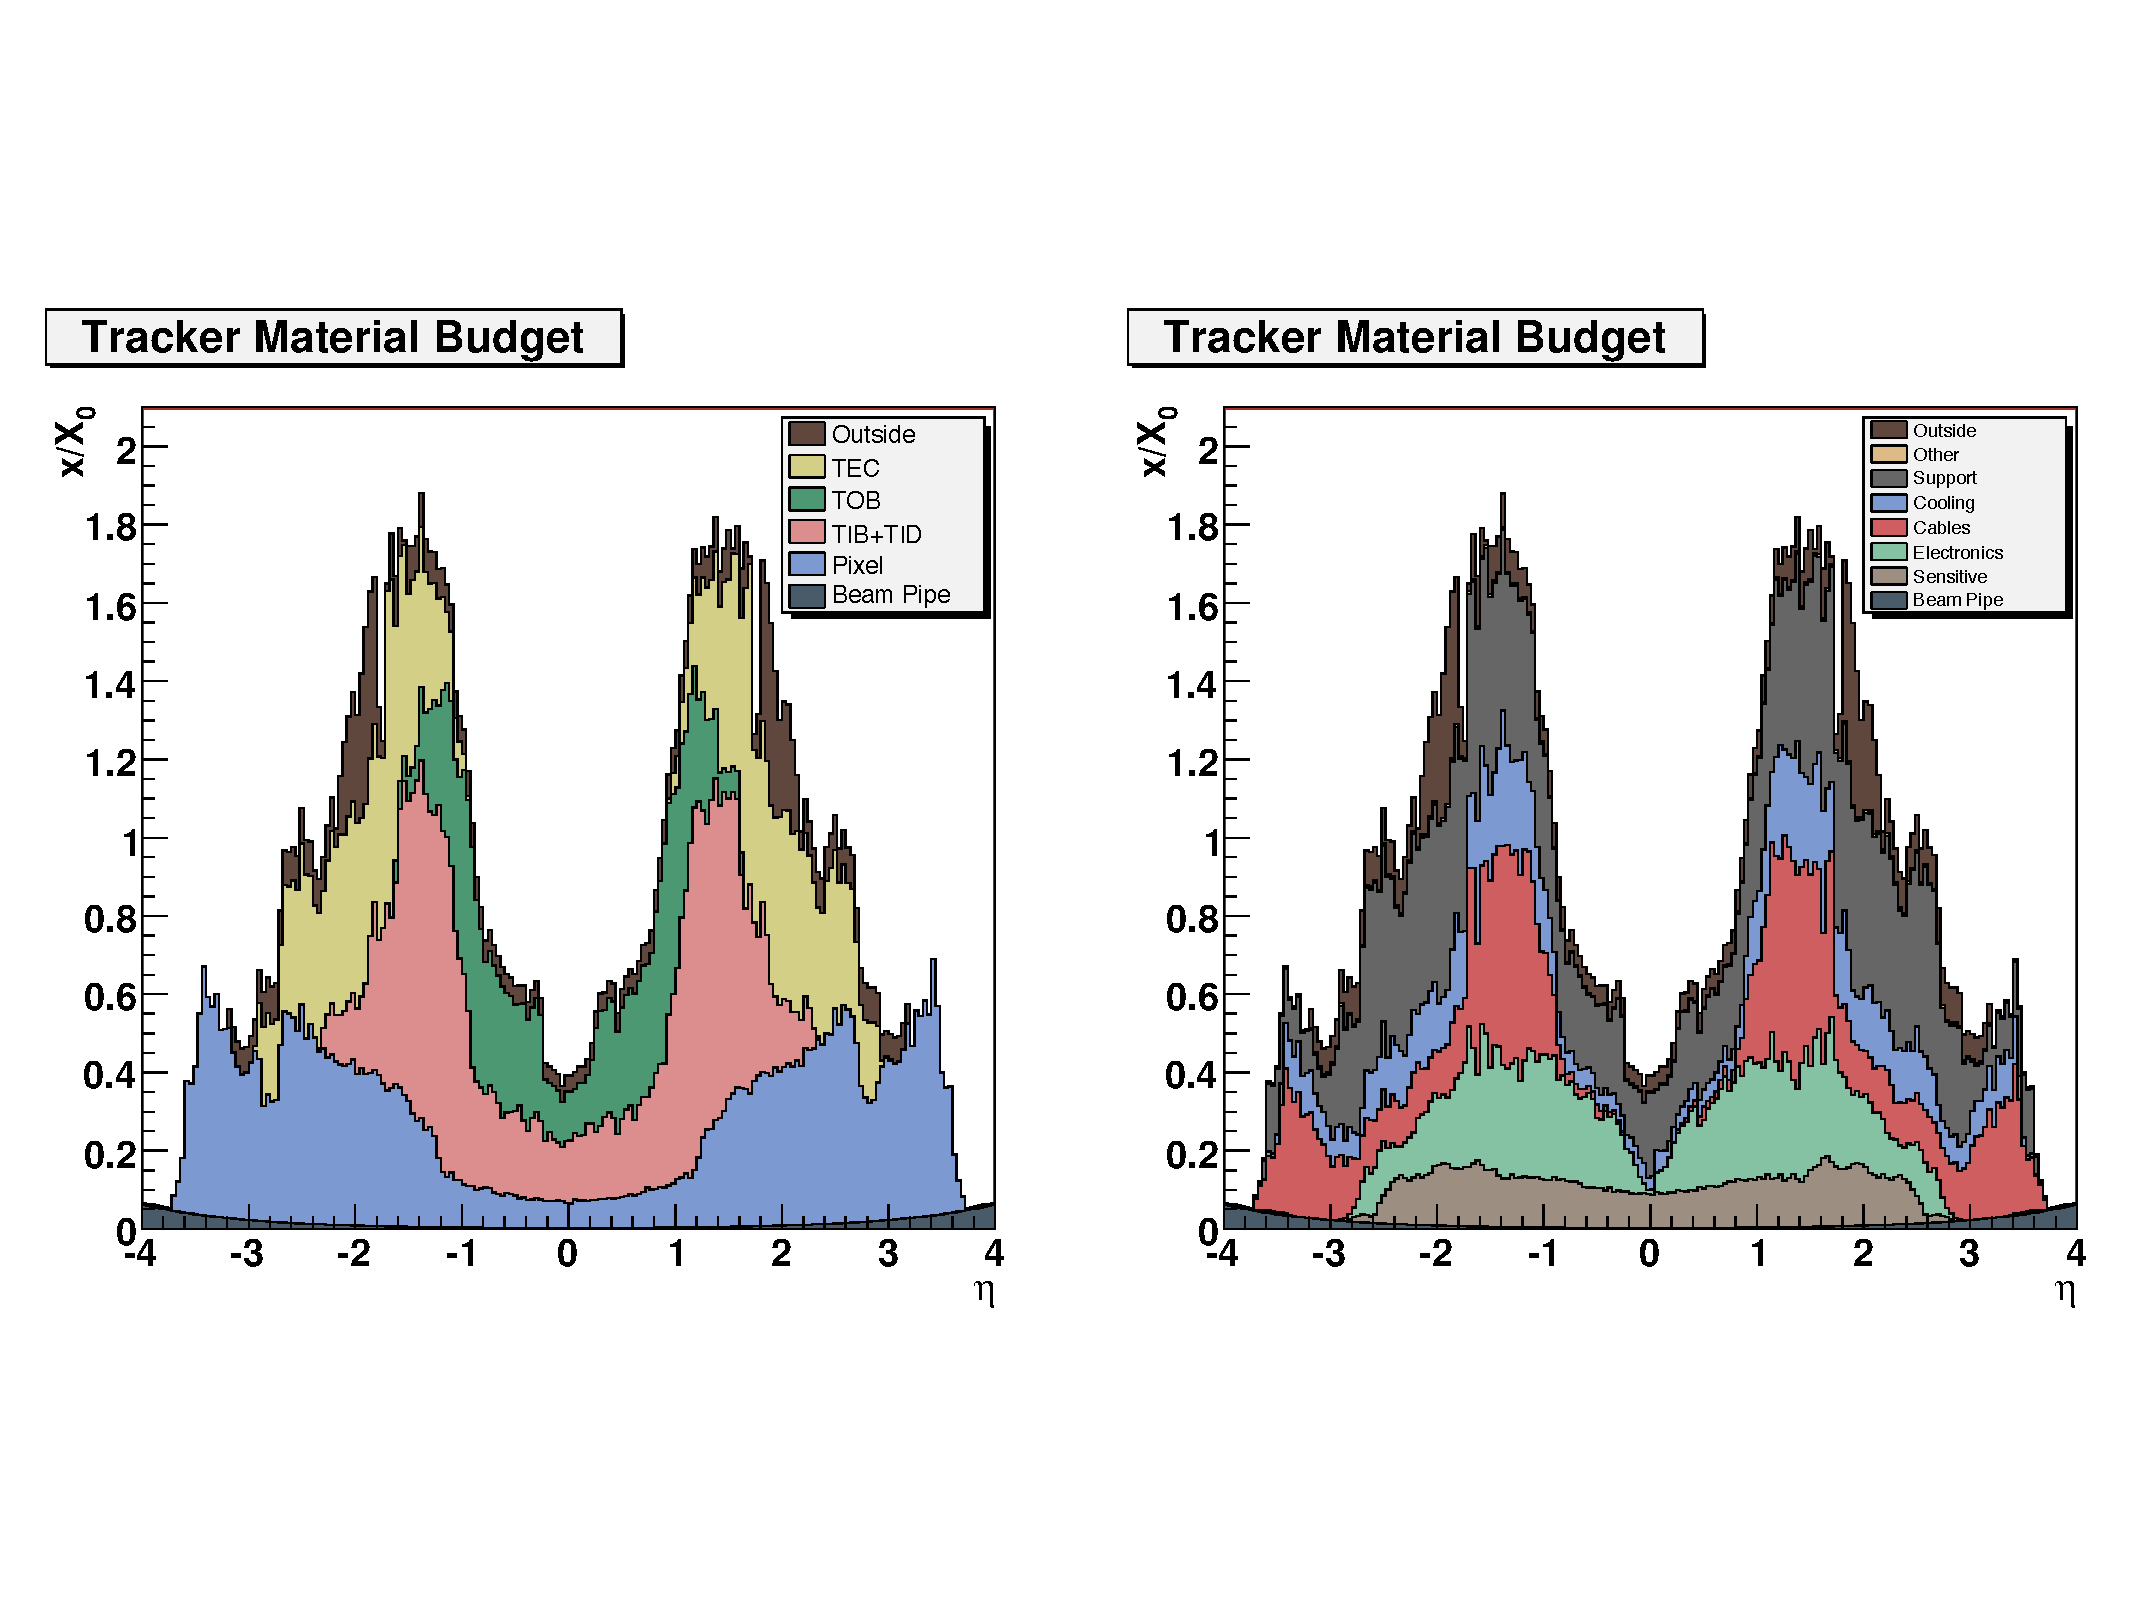
\includegraphics[width=0.99\textwidth]{CMS_DetectorFigures/TrackerMaterialBudget.pdf}
 \caption{Material budget of the CMS tracker in units of radiation
   length as a function of pseudorapidity $\eta$ for the (left)
   different subdetectors and (right) functional contributions.\label{fig:materialBudget}}
\end{figure}
\subsection{Pixel Tracker}
The inner pixel detector is composed of three 53-cm-long cylindrical layers at a
radii of 4.4, 7.3, and 10.2 cm -- which is called BPix. It is finalized by two disks of pixel
modules at each side extending from approximately 6 to 15 cm in
radius -- which is called FPix. The barrel is composed of 672 full and 96 half modules, a full (half)
module is composed of 16 (8) read-out chips equipped with 52$\times$80 pixels
of size 100$\times$150 $\mu$m. A completed full-module has the
dimensions of 66 mm$\times$26 mm and is provided with readout and
power. Figure~\ref{fig:Bpix} shows a completed full- and half- module as
well as an schematic of the different component integrated in the
module. The two disks at each side of the pixel barrel (see
Figure~\ref{fig:trackerlayout}) is composed 24 modules -- with a
trapezoidal geometry. Each disk is composed of two different
panel types; the first and closest to the interaction point is formed
by a 1$\times$2, 2$\times$3, 2$\times$4, and 1$\times$5 plaquettes
amounting to a total of 21 read-out chips; the second and furthest from
the interaction point is formed by a 2$\times$3, 2$\times$4, and 2$\times$5 plaquettes
amounting to a total of 24 read-out chips. A plaquette is the basic
unit of the FPix and consist of a single pixel sensor bump-bonded to
the read-out chip and wired-bonded to a very-high-density-interconnect
(VHDI) that provides data connections, power, and
control. Figure~\ref{fig:Fpix} show an schematic of these two
different panels as well as a photograph of a finalized
panel. Finally, a layout of the pixel traker system is given in
Figure~\ref{fig:PixelLayout} as well as the a detection efficiency as
a function of the pseudorapidity. The total number of pixels in the
pixel tracker is about 66 millions and they are equivalent to an area
of about 1 m$^2$.
\begin{figure}
 \centering
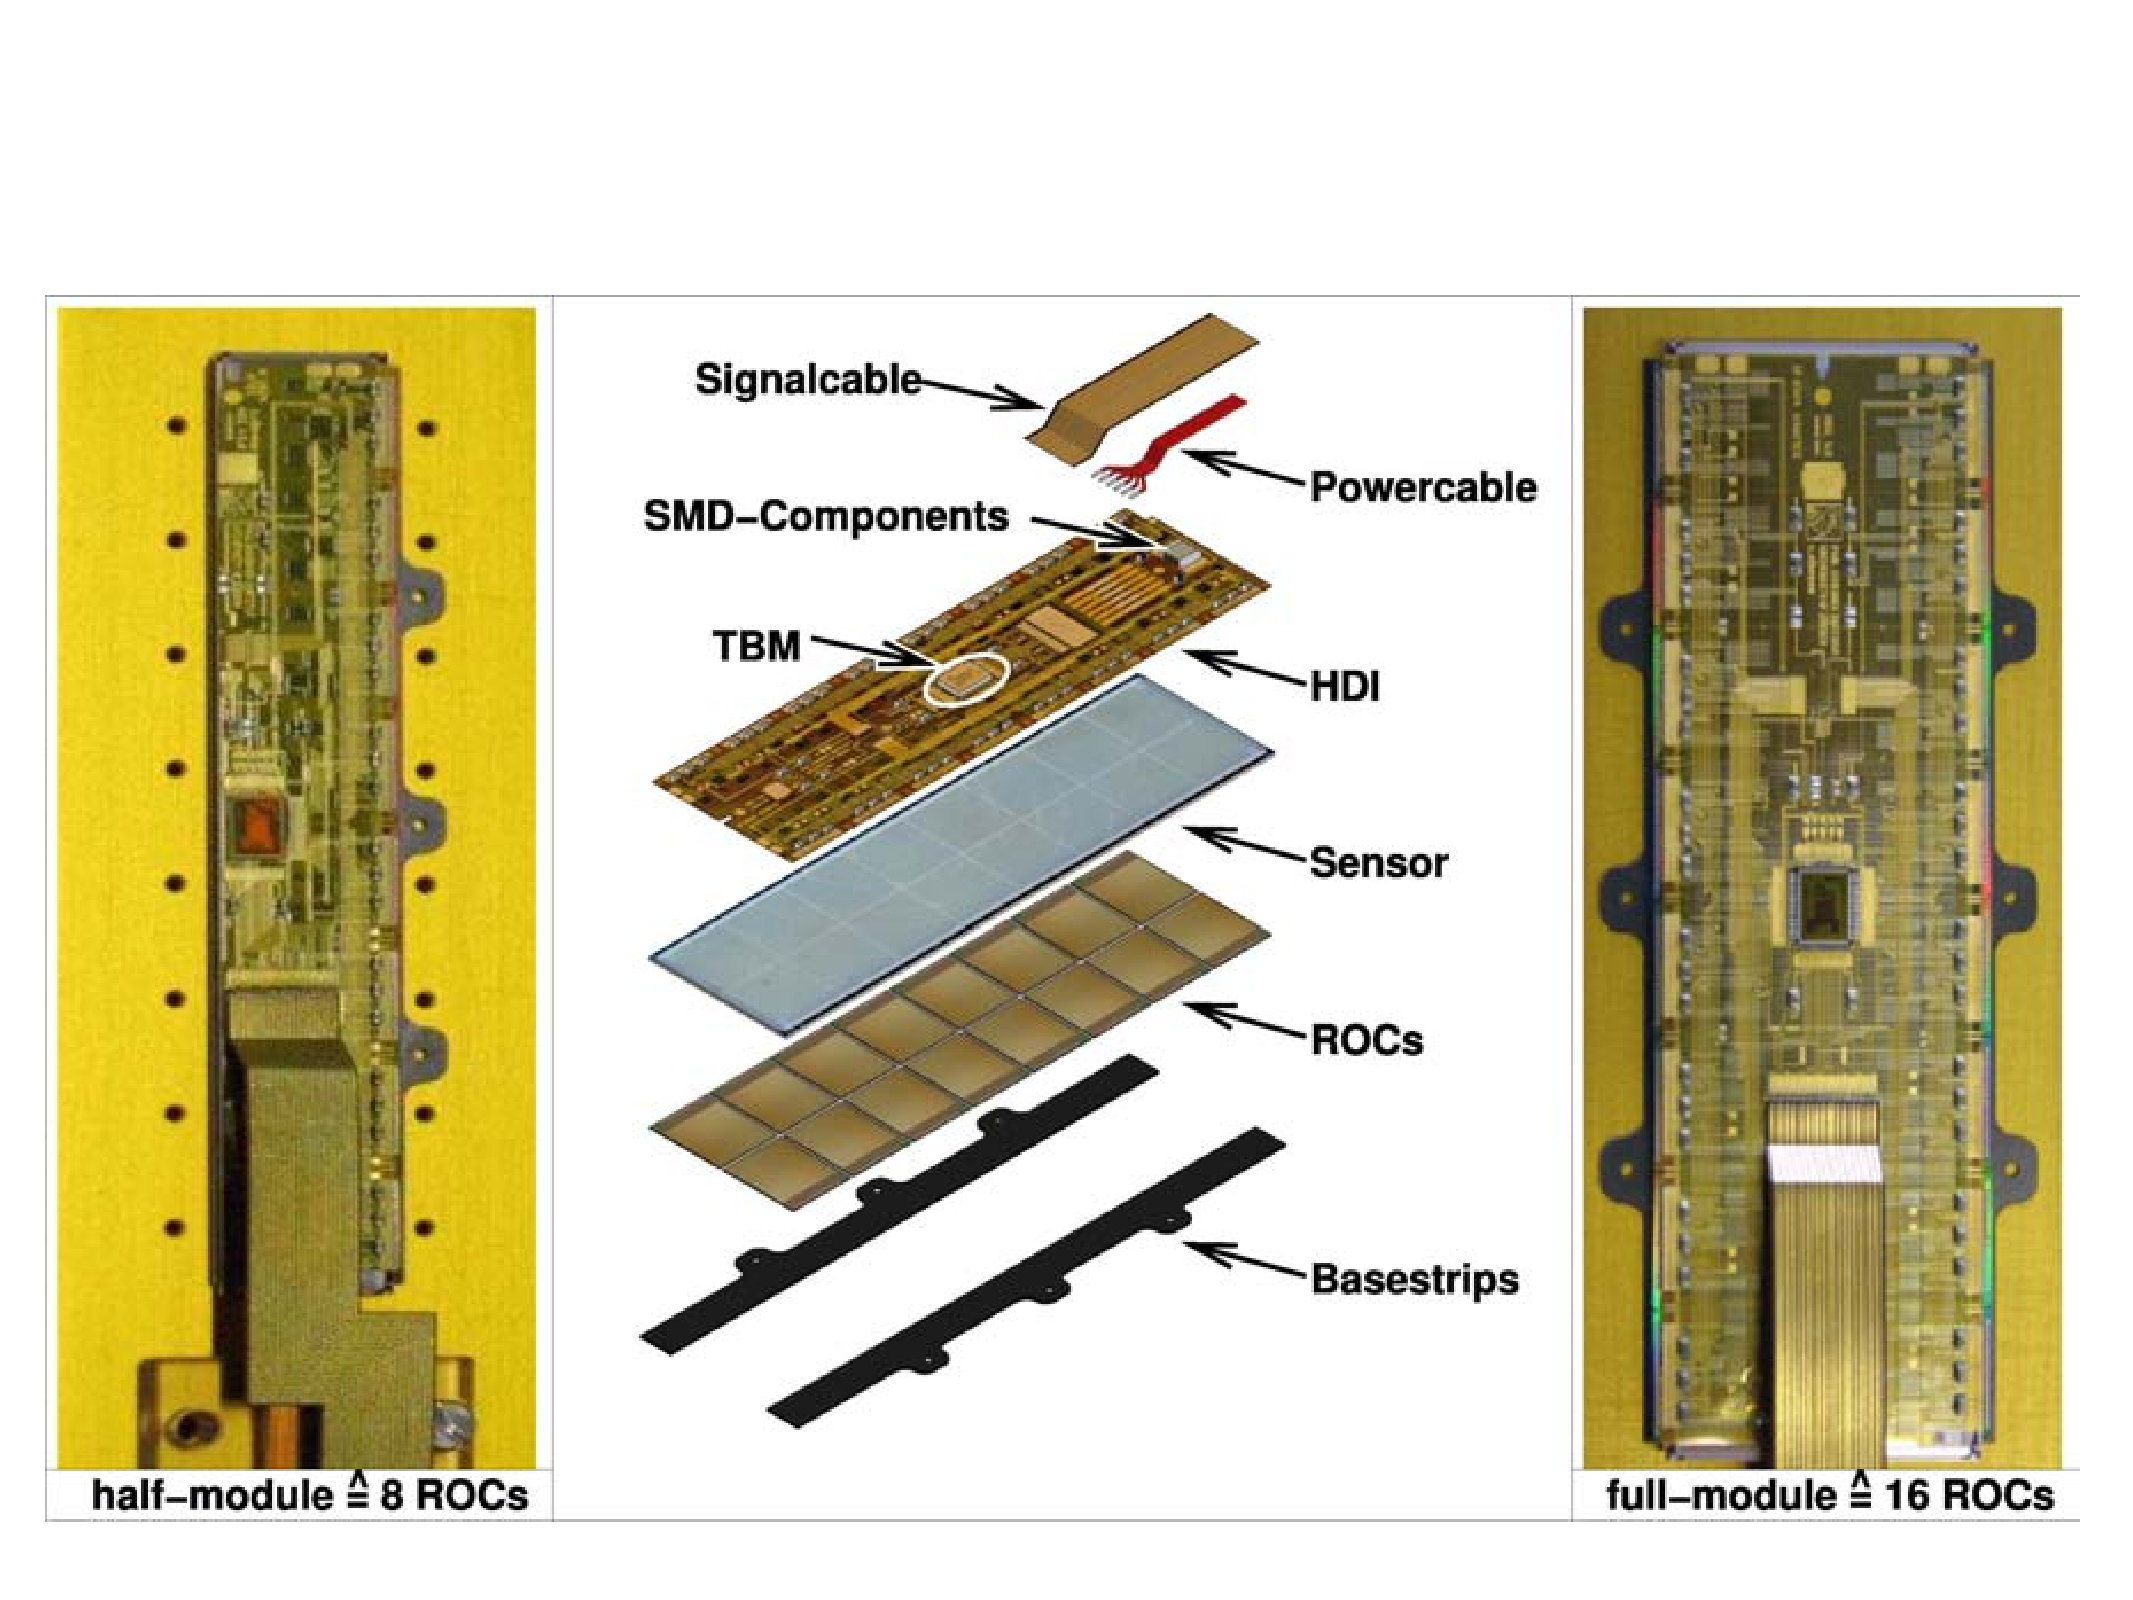
\includegraphics[width=0.99\textwidth]{CMS_DetectorFigures/BPixModule.pdf}
 \caption{BPix completed modules; (left) half-module, (center) an
   schematic of the different component forming the a full-module,(right) full-module.\label{fig:Bpix}}
\end{figure}
\begin{figure}
 \centering
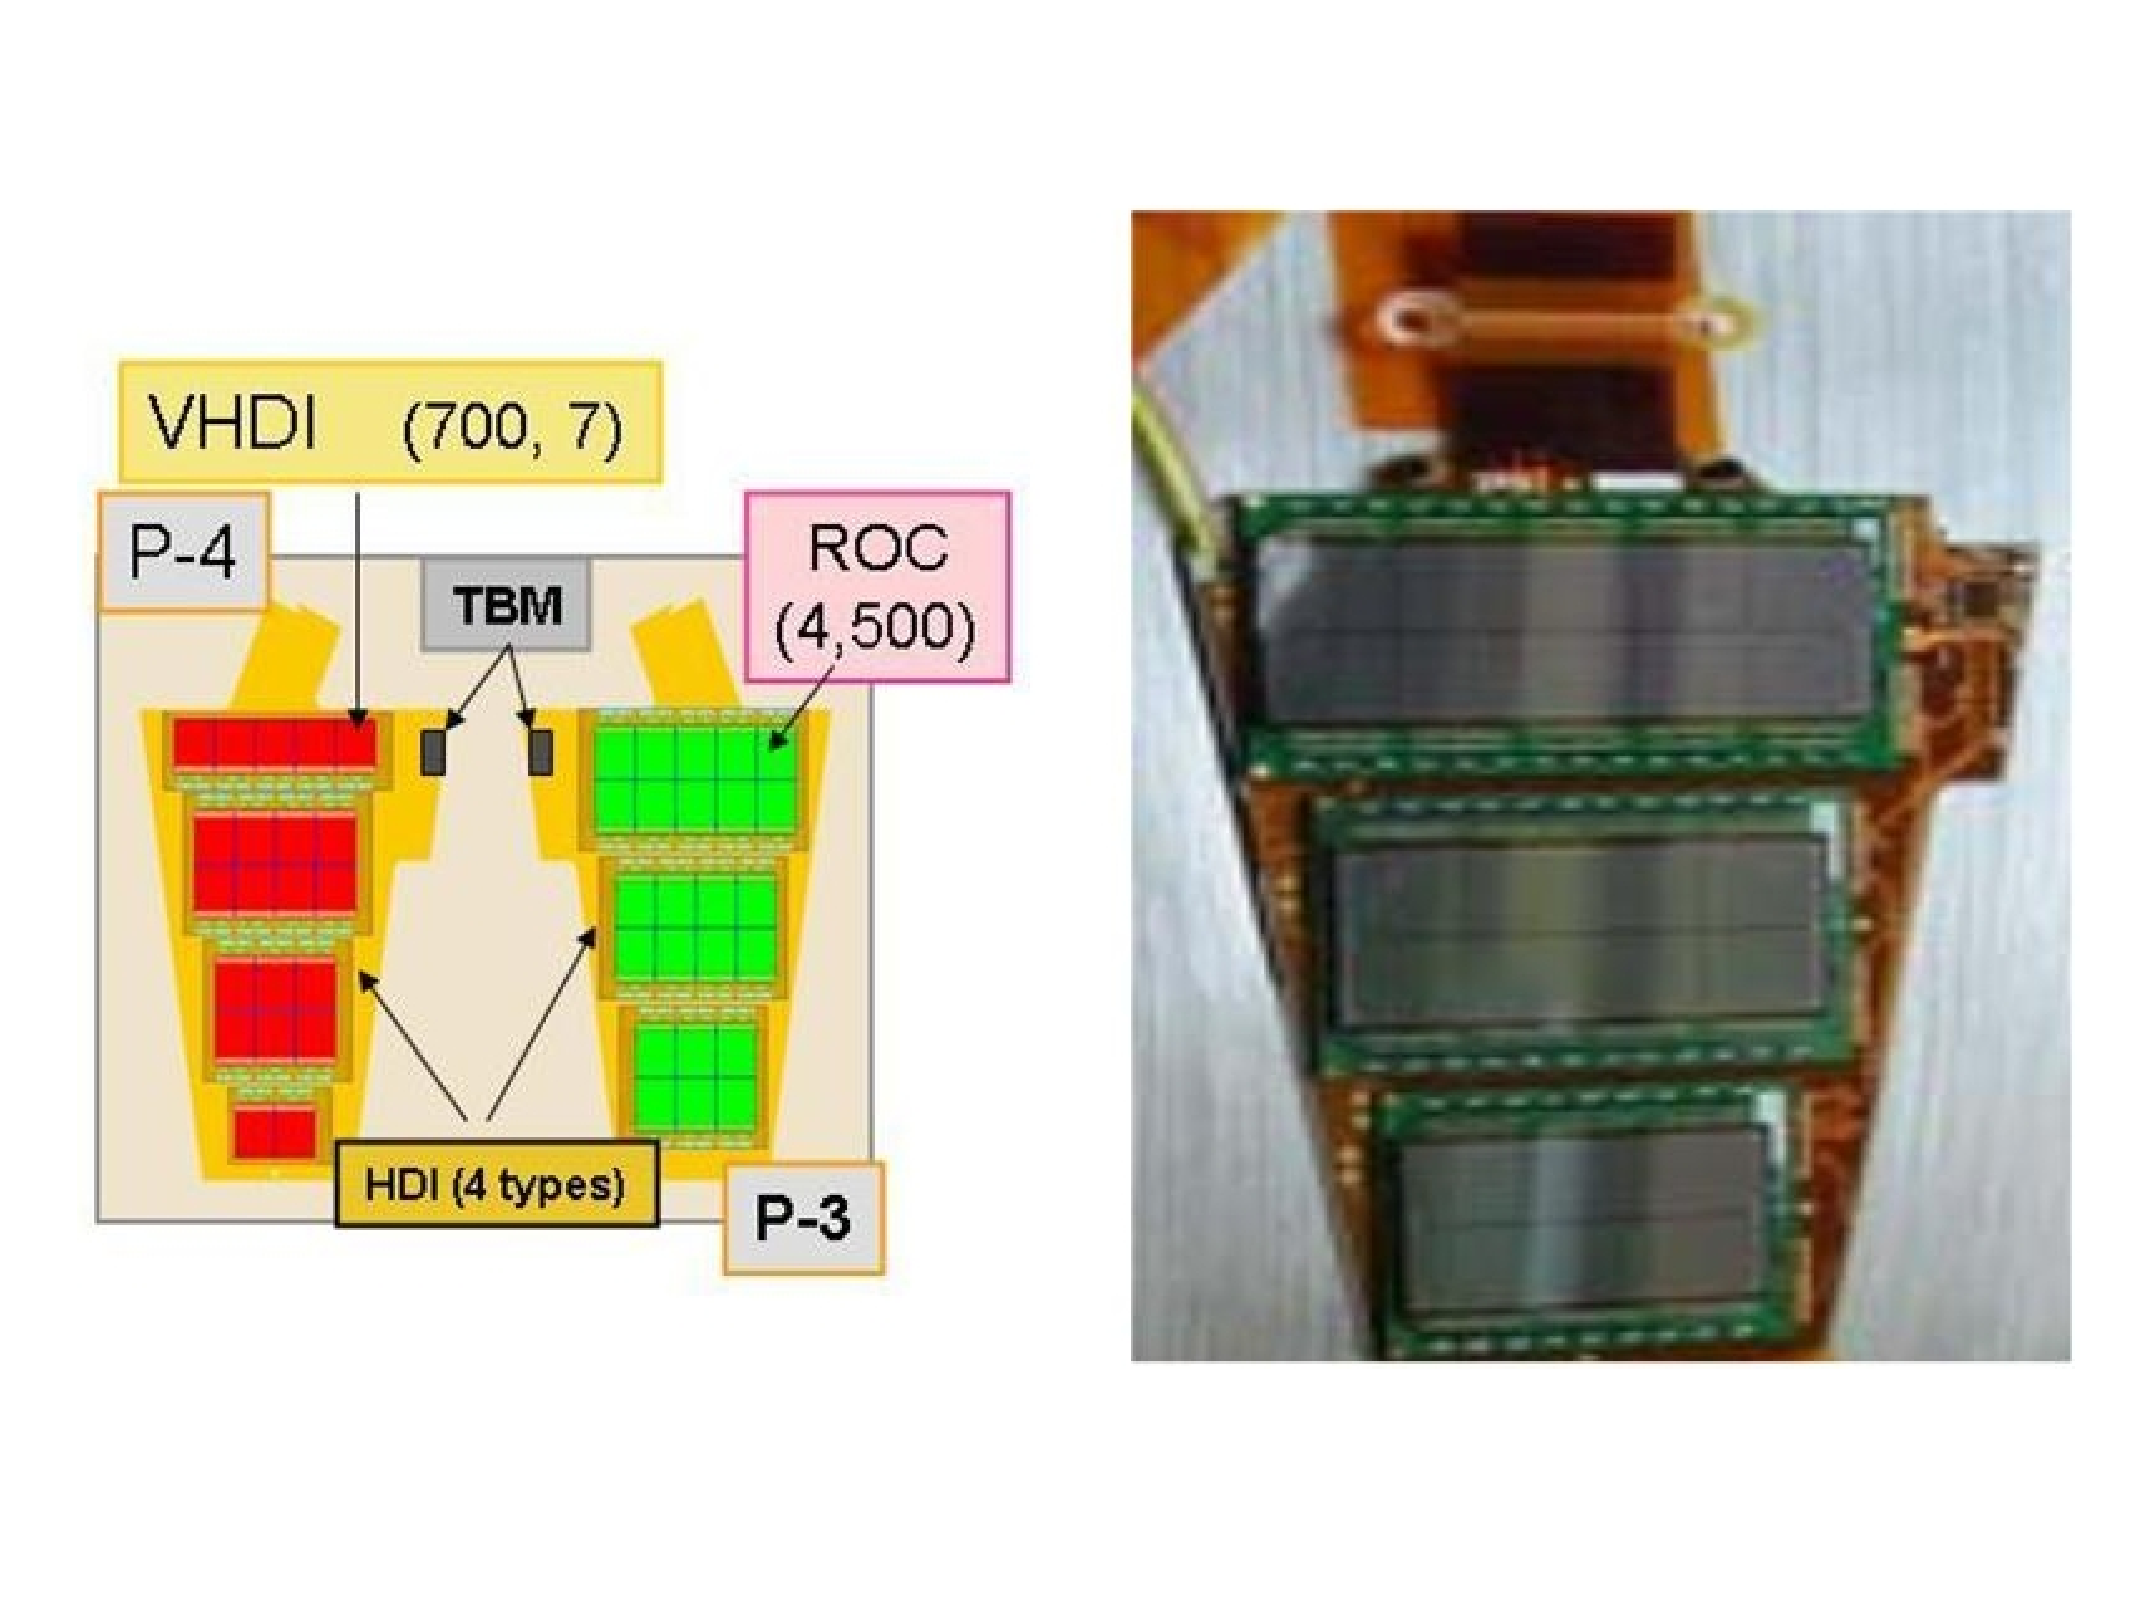
\includegraphics[width=0.99\textwidth]{CMS_DetectorFigures/FPixModule.pdf}
 \caption{FPix module; (left) an schematic of the two types of module,
   (right) a photograph of one of the completed FPix modules.\label{fig:Fpix}}
\end{figure}

\begin{figure}
 \centering
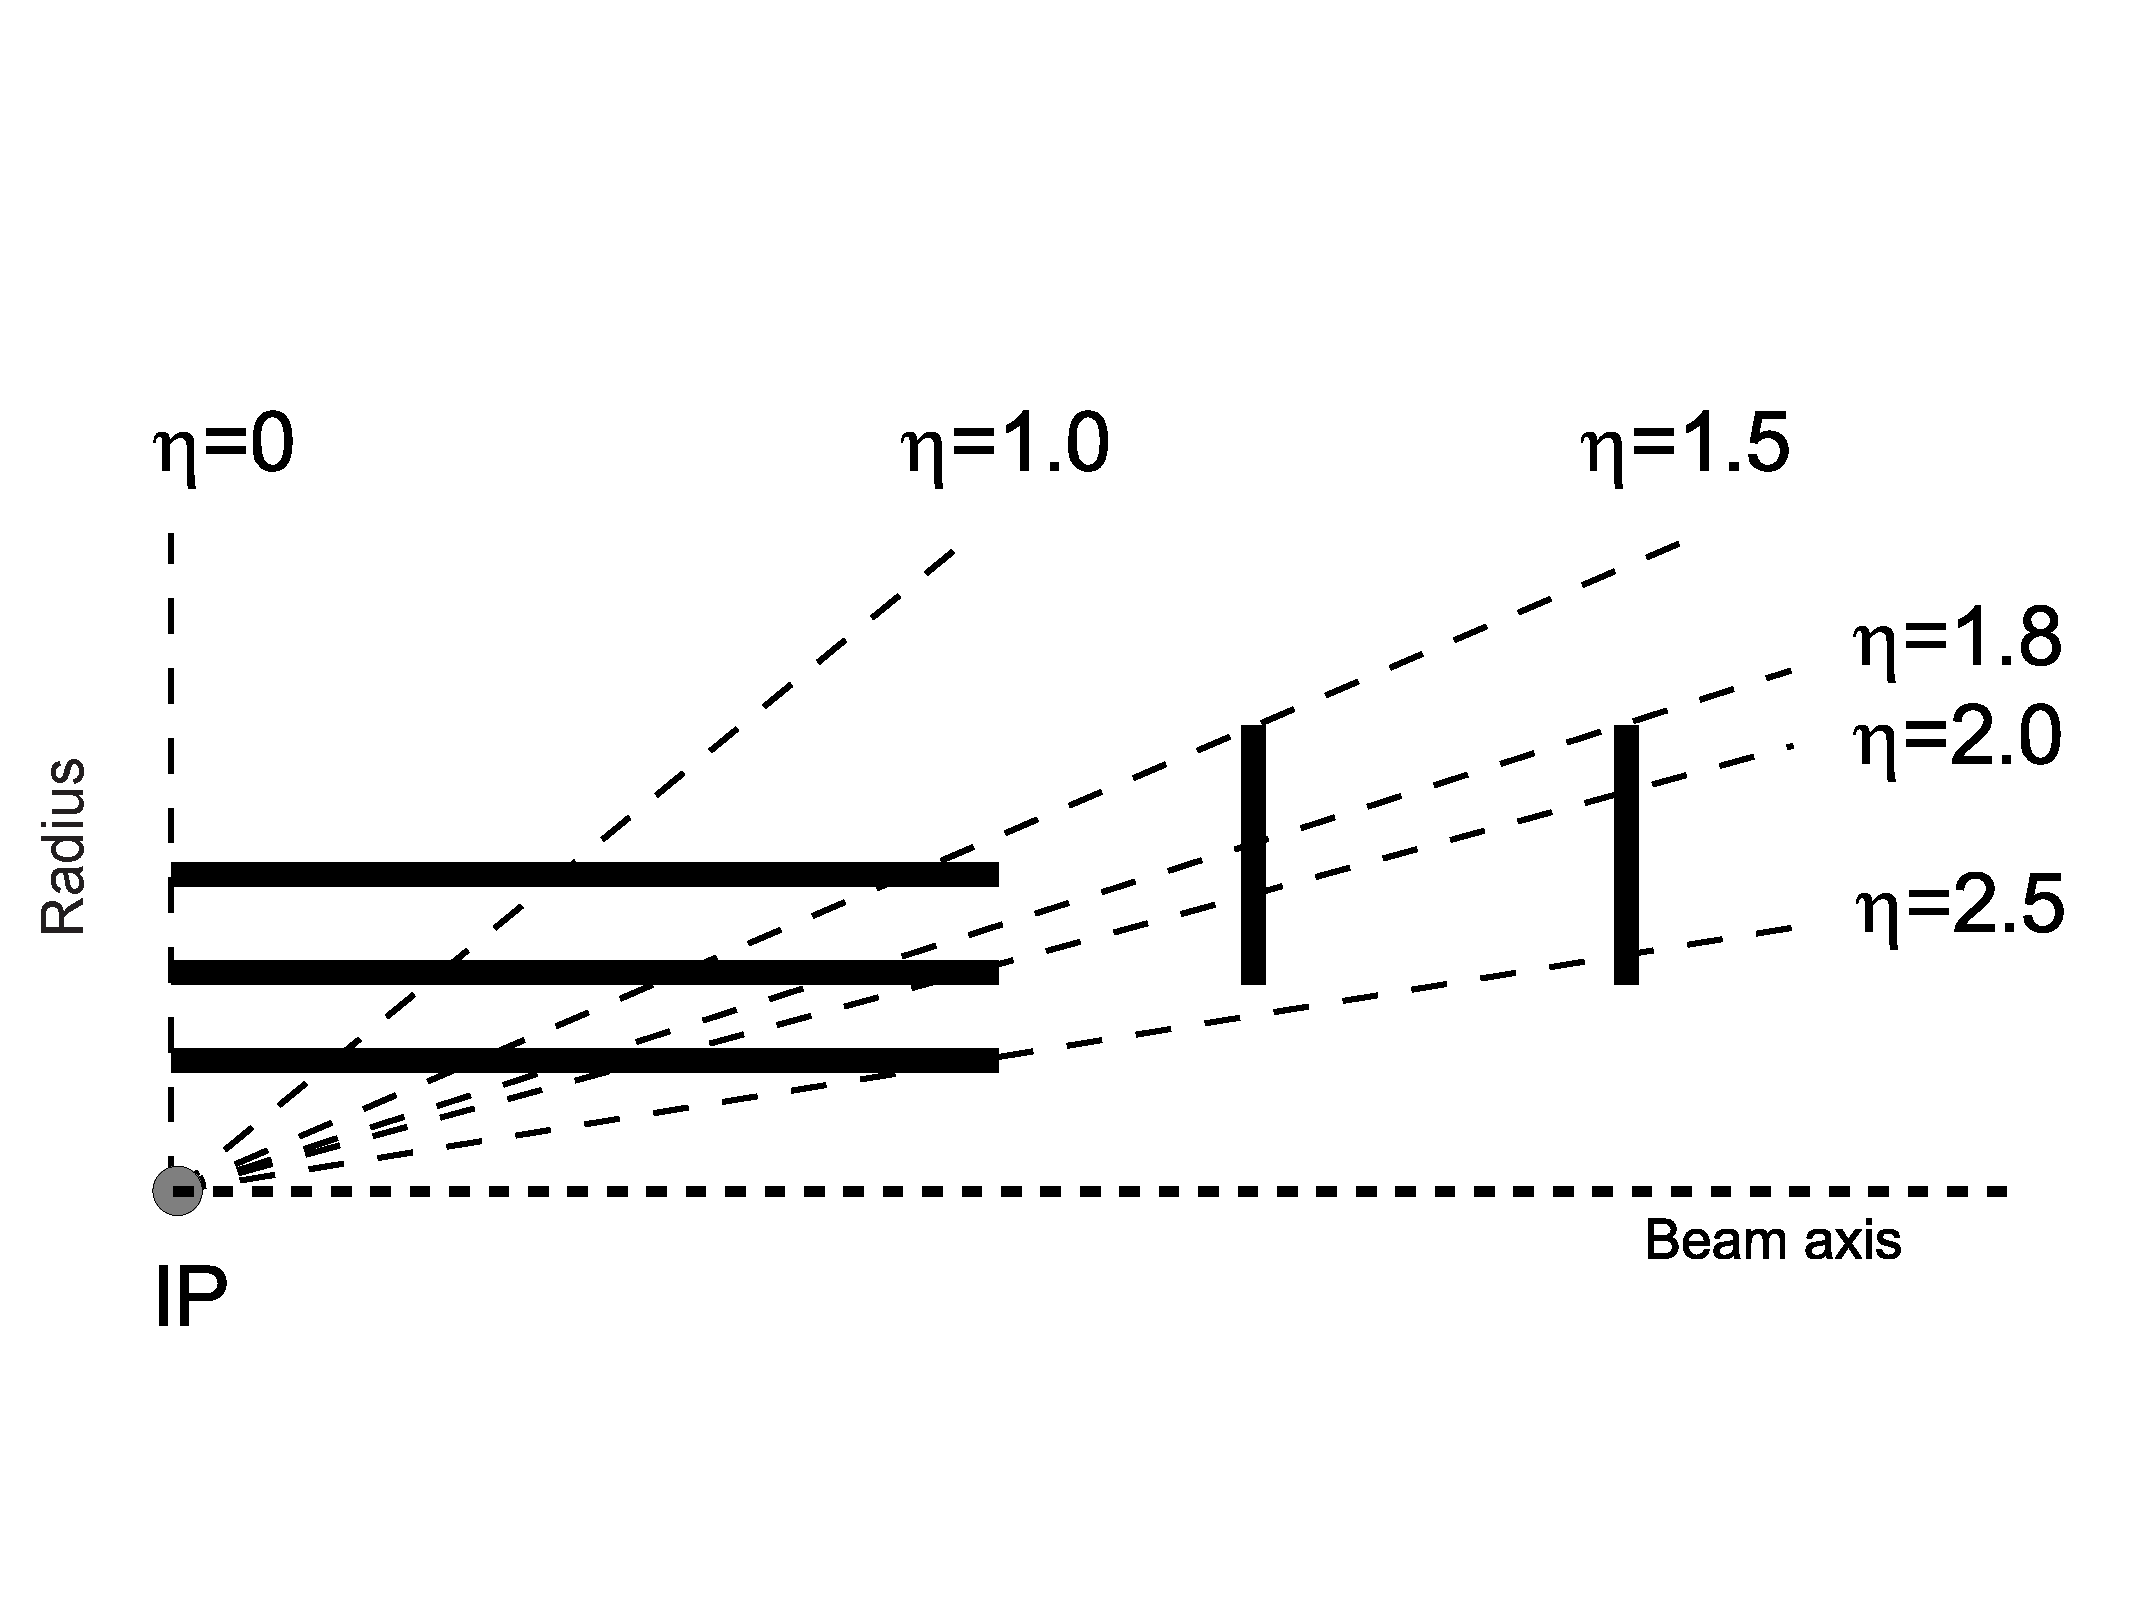
\includegraphics[width=0.49\textwidth]{CMS_DetectorFigures/PixelLayout.pdf}
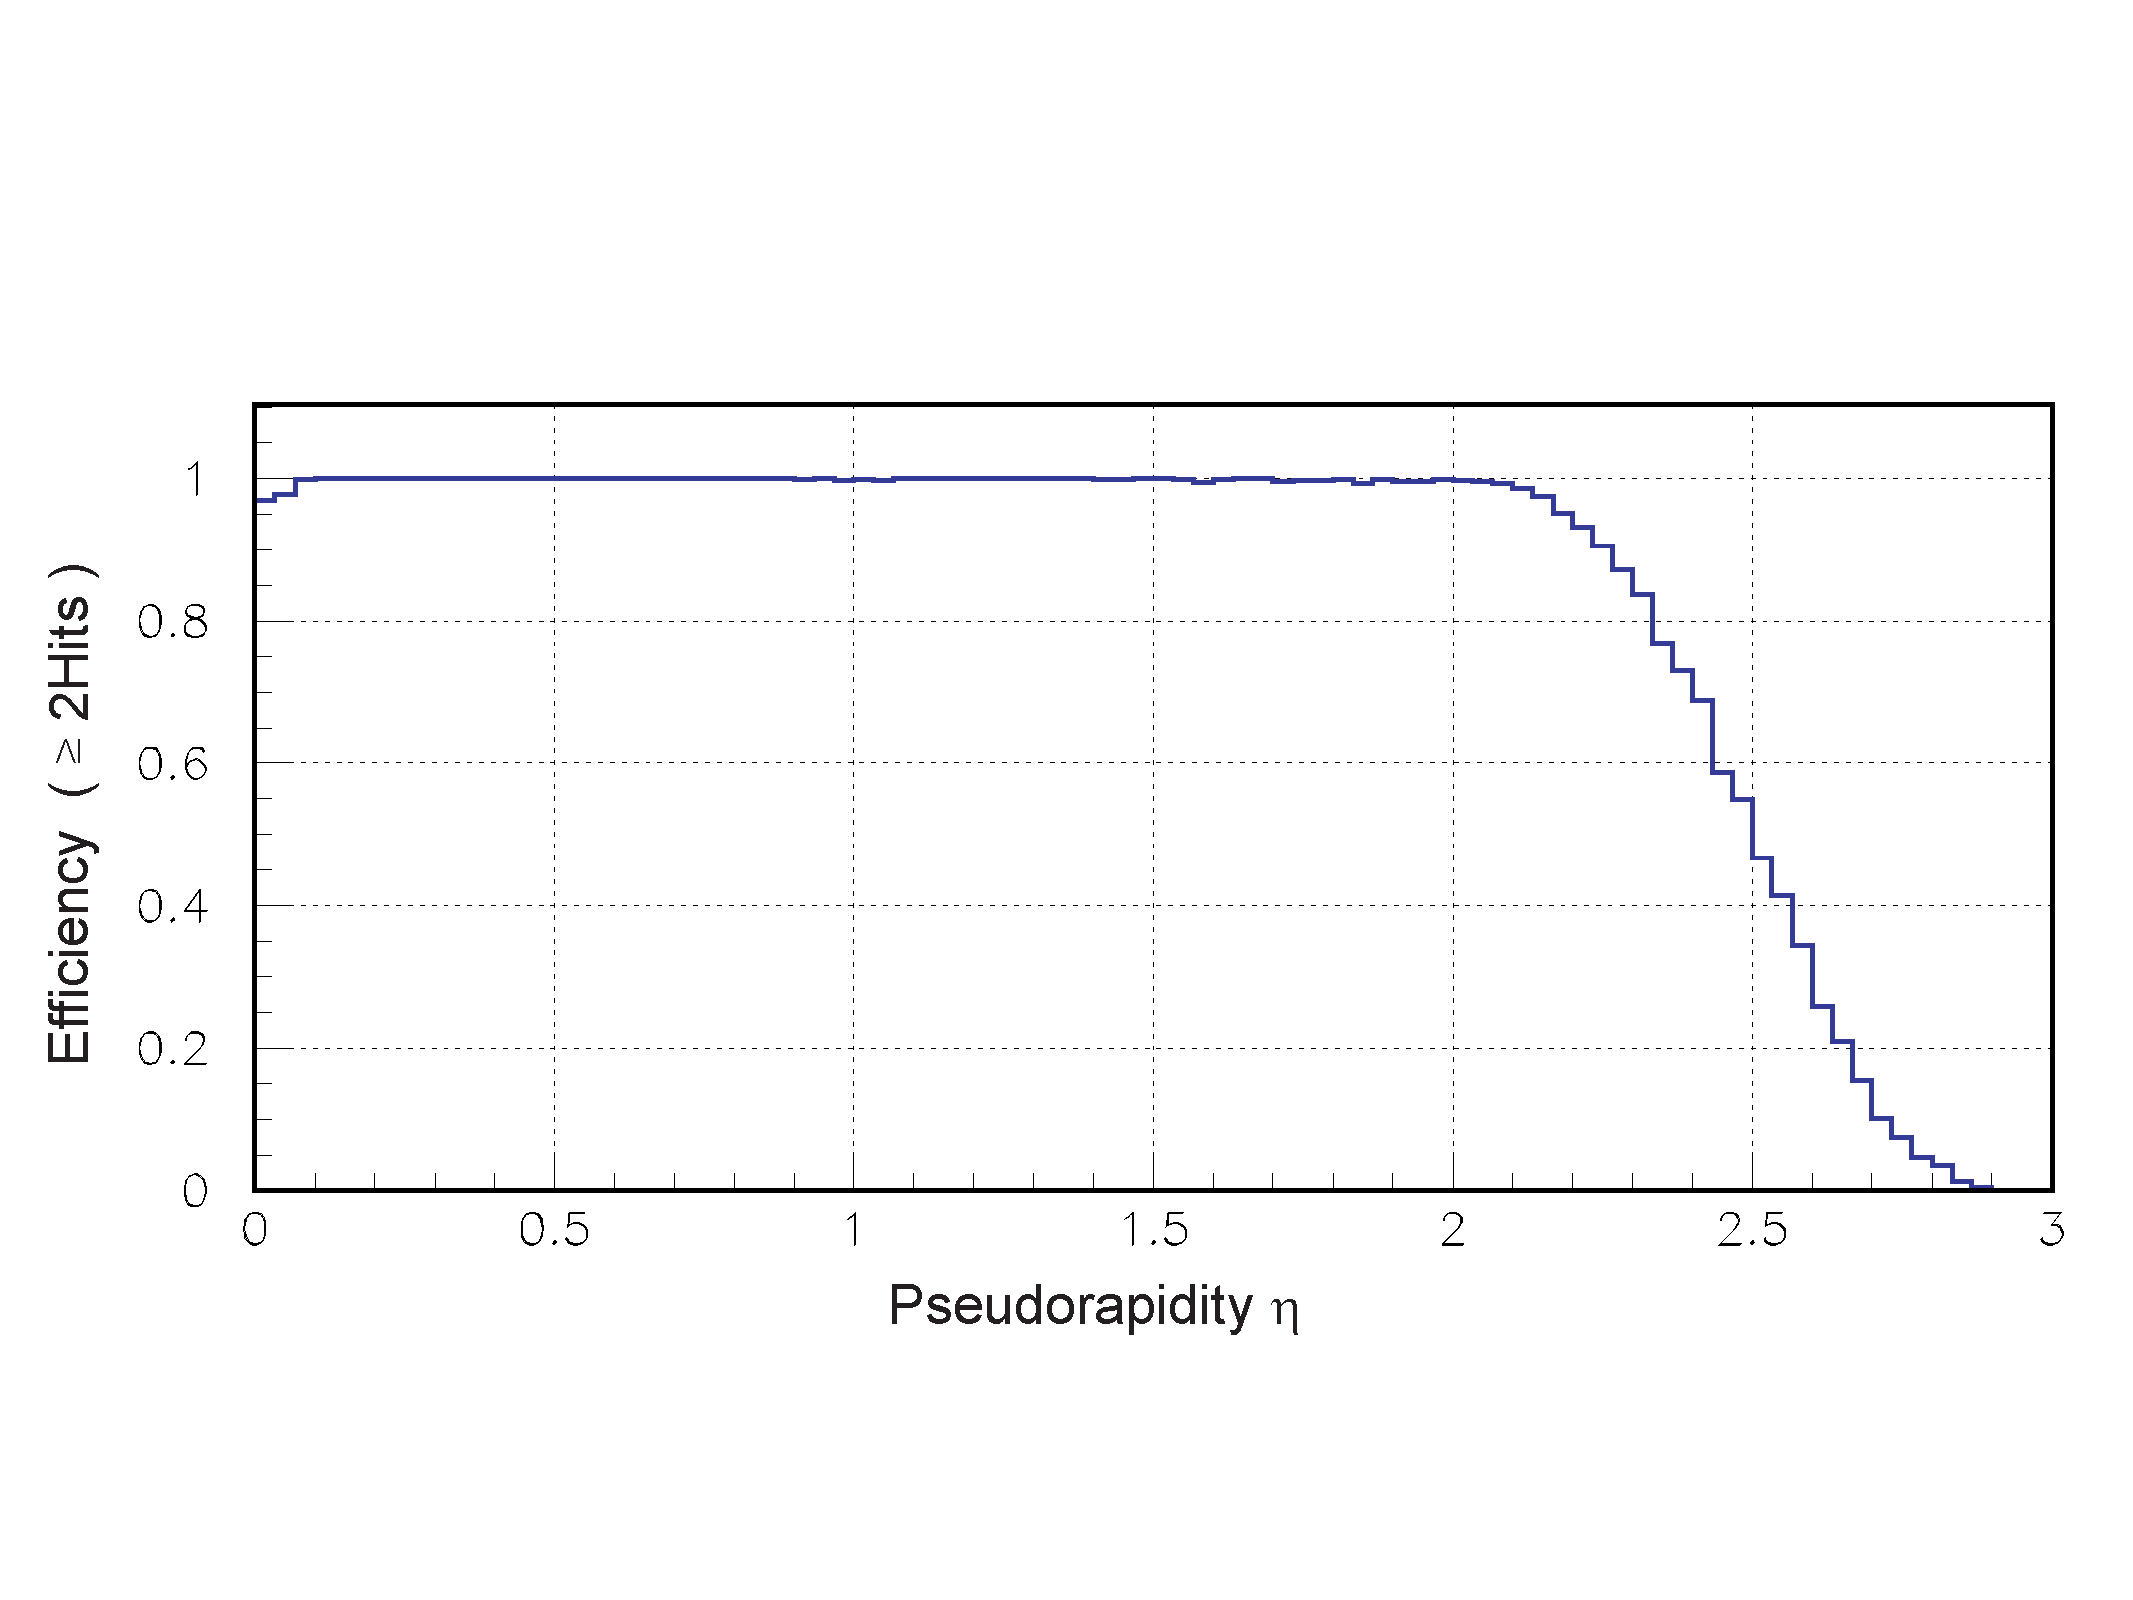
\includegraphics[width=0.49\textwidth]{CMS_DetectorFigures/PixelEfficiency.pdf}
 \caption{(Left) the layput of the silicon pixel tracker, (right) the
   pixel tracker detection efficiency as a function of the pseudorapidity.\label{fig:PixelLayout}}
\end{figure}
\subsection{Strip Tracker}
The silicon tracker is located outside the inner pixel tracker and is
composed of three subsystems that extend from 20 cm to 116 cm in the
radial direction. The Tracker Inner Barrel and Disks (TIB/TID) are
the innermost subsystem extending up to a radius of 55 cm, it includes
4 barrel layers and 3 disks at each side. The TIB/TID with their 320
$\mu$m thick silicon micro-strip sensor oriented along the $z$-axis records up to 4 $r$-$\phi$
measurements on a particle's trajectory. The strips pitch  in the TIB -- the
distance between each strip -- varies between 80 $\mu$m and 120 $\mu$m
in layers 1-2 and 3-4, respectively. The resulting single point
resolution is therefore 23 $\mu$m and 35 $\mu$m for the 1-2 and 3-4
layers, respectively. The TID has strip pitches between 100 -140$\mu$m
-- resulting in single point resolution between 29-41 $\mu$m. The
TIB/TID is completely sorrounded by the Tracker Outer Barrel (TOB)
which with its 6 barrel layer extends up to a radious of 116 cm. The
layers are composed of 500 $\mu$m thick micro-strips sensor with
pitches of 183 $\mu$m and 122 $\mu$m for the firts 4  and last 2
layer, respectively -- recording up to 6 $r$-$\phi$
measurements on a particle's trajectory with single point resolutions of 53 $\mu$m
and $\mu$m, respectively. The TIB/TID and the TOB cover the region
with $|z|< 113$ cm, beyond this point (see
Figure~\ref{fig:trackerlayout}) the Tracker EndCaps (TEC$^{\pm}$) --
where the sign, obiously, represents the position on the $z$-axis --
extend from 124 cm $|z|< 282$ cm and 22.5 cm $|r|< 113.5$ cm. The TEC
consists of 9 disks which contains up to 7 rings of silicon
micro-strips, the later are 320 $\mu$m and 500 $\mu$m thick in the
inner 4 and outer 3 rings, respectively.
Additionally, modules in the two innermost layers in the TIB and TOB,
the two inner most rings of the TID, as well as rings 1,2 and 5 of the TECs are
equipped with a second micro-strip detector module that is mounted
back-to-back allowing measurements on the perpedicular coordinate --
i.e. $z$ and r in the barrel and the disks, respectively. In this
fashion at least $\approx$ 9 hits in the silicon strip tracker in the
$|\eta|<2.4$ range are ensure, with at least $\approx$ 4
two-dimensional measurements. The full strip tracker amounts to a
total of 9.3 million strips and covers an active are of silicon equal
to 198 m$^2$.

\subsection{Performance of the CMS Tracker}

The tracker efficiency for single muons is measured in 7\TeV data as a
function of the muon pseudorapidity $\eta$ and the number of
reconstructed vertices using the tag-and-probe technique on muons
decaying from Z bosons. The results are shown in
Figure~\ref{fig:MuonEfficiency}, where the muon efficiency is above
99\% within the tracker acceptance and up to 20 reconstructed
vertices. The muon transverse momentum and transverse impact
paramenter resolution as a function of  $\eta$ are estimated from the
CMS full simulation, the results are shown in left and right panel of
Figure~\ref{fig:MuonResolution}, respectively. The muon transverse
momentum resolution is about 1-3\% for $|\eta|<1.5$ for muons of
different energies. The transverse impact parameter is estimated to be
between $\sim$10-20 $\mu$m for a 100\GeV muon while the for 1\GeV muons the
resolution is between $\sim$ 80-250 $\mu$m.

\begin{figure}
 \centering
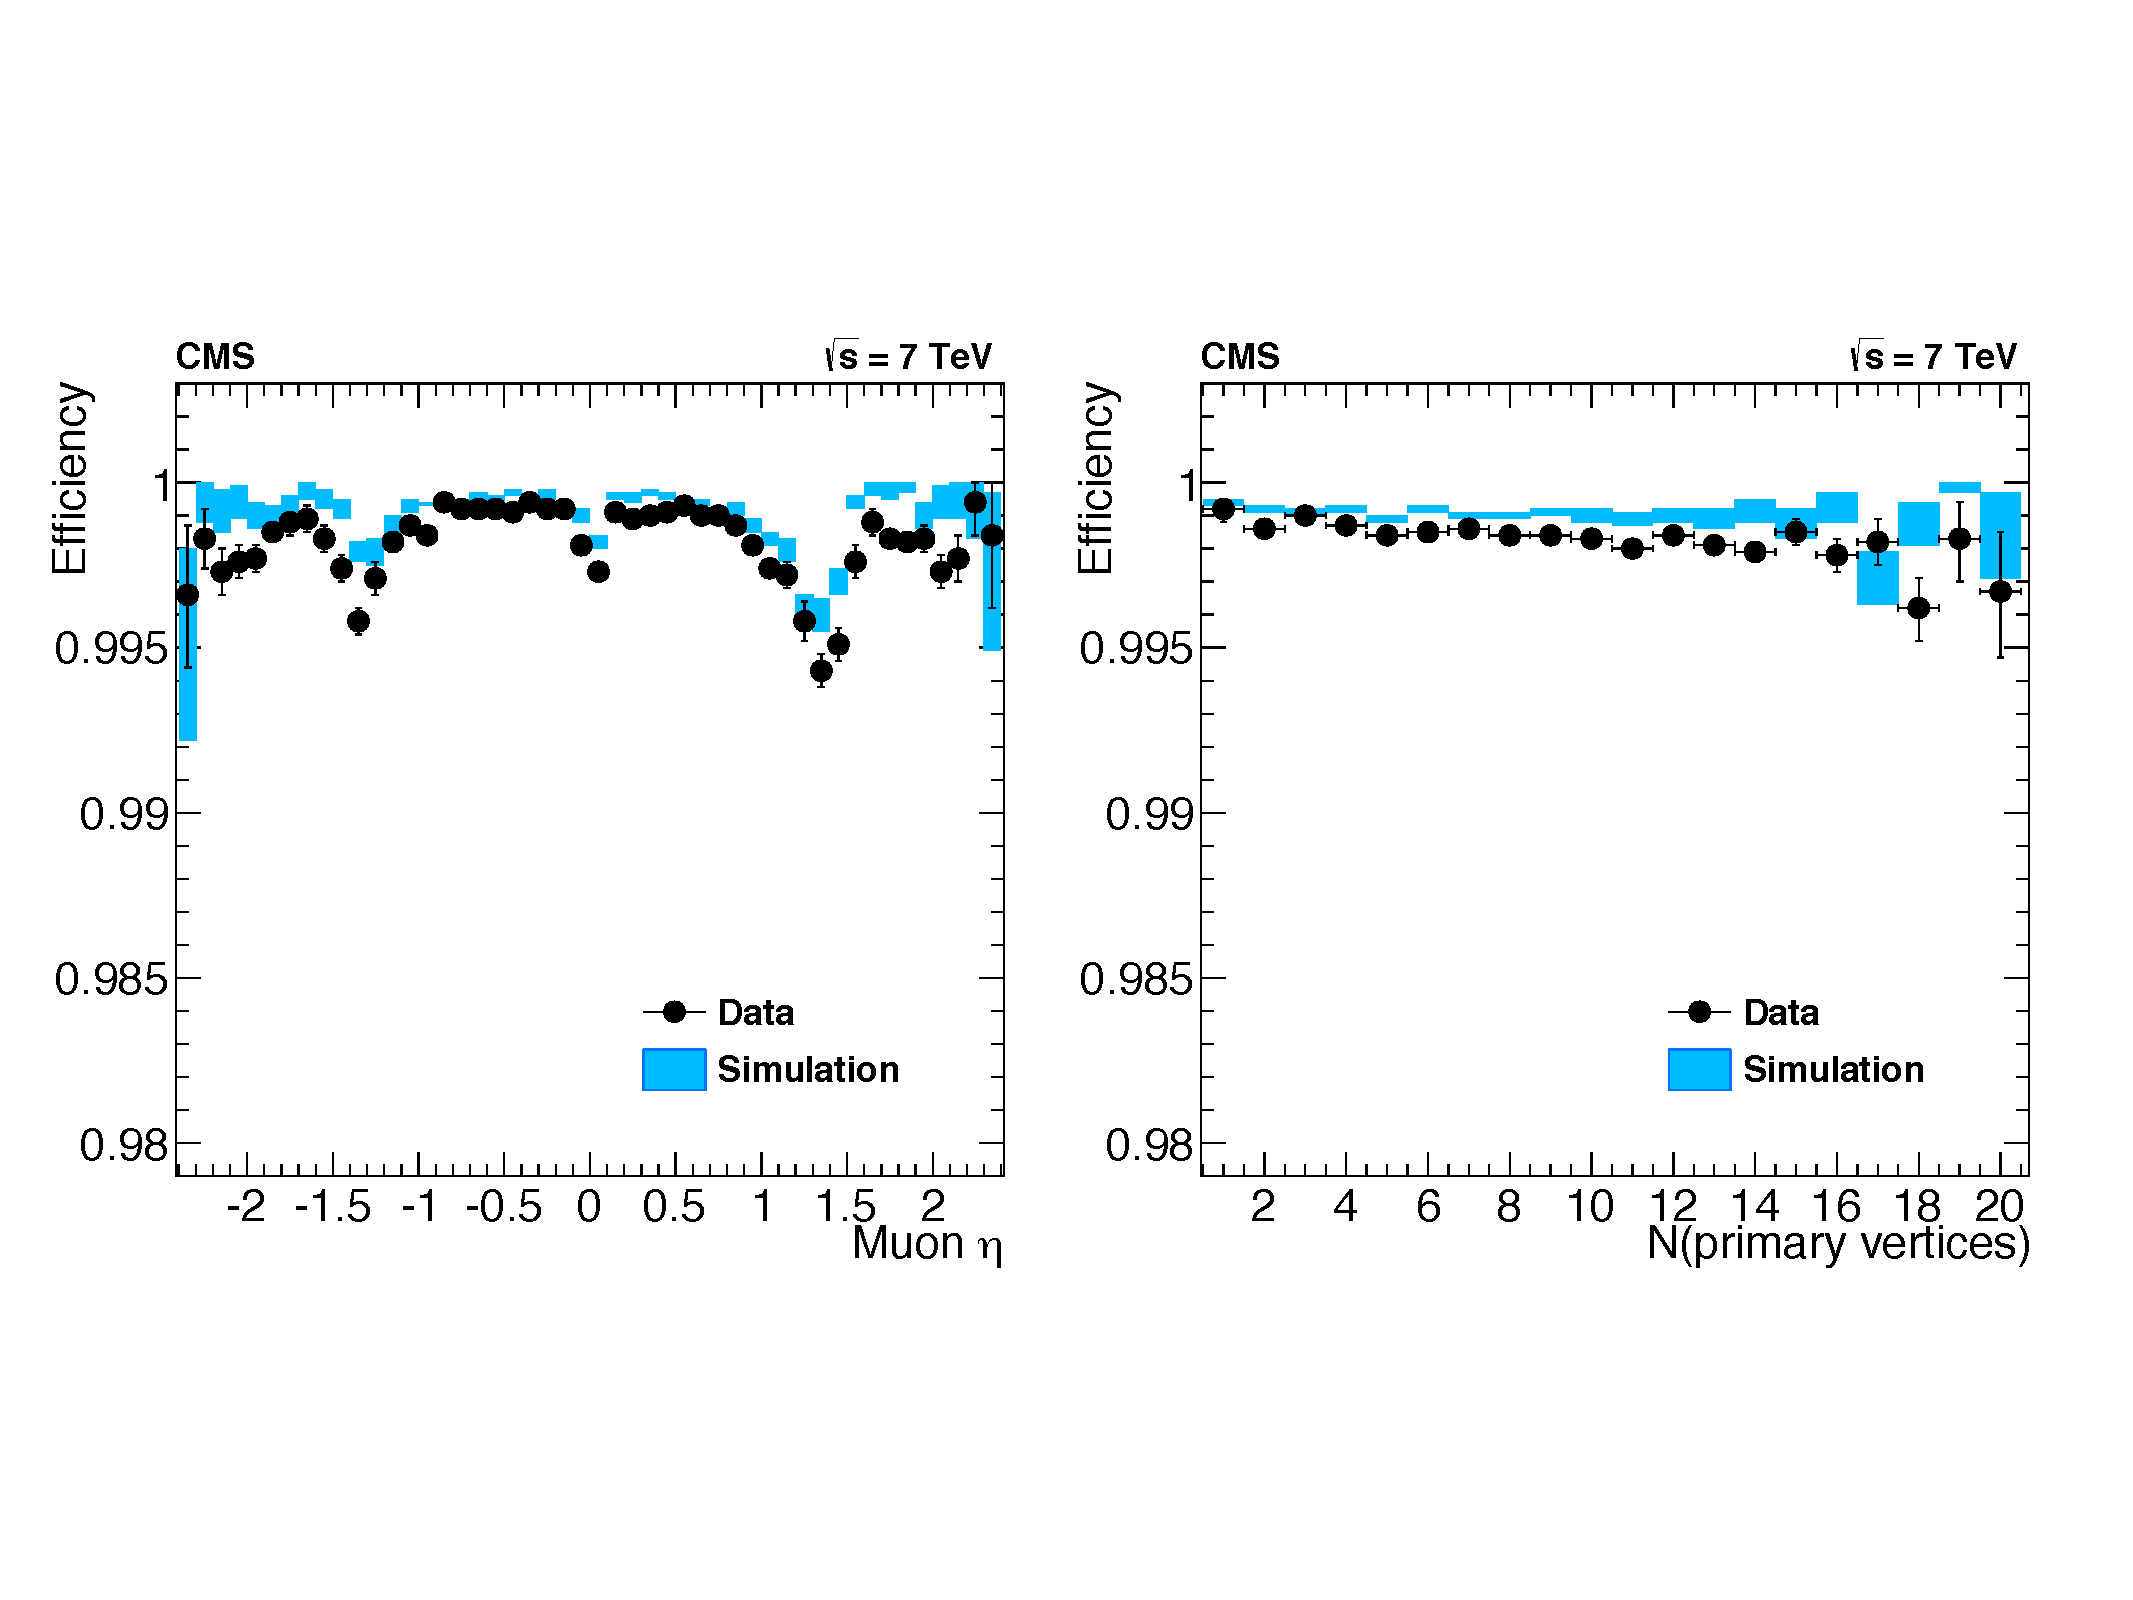
\includegraphics[width=0.99\textwidth]{CMS_DetectorFigures/TrackerMuonEff.pdf}
\caption{Tracking efficiency for muons from Z decays using the tag-and
 -probe technique. The left panel and right panel show the efficiency
 as function of the muon $\eta$ and the number of reconstructed
 vertices, respectively. The black dots represent the measurement in
 7\TeV data and the solid color represents the CMS simulation.\label{fig:MuonEfficiency}}
\end{figure}

\begin{figure}
 \centering
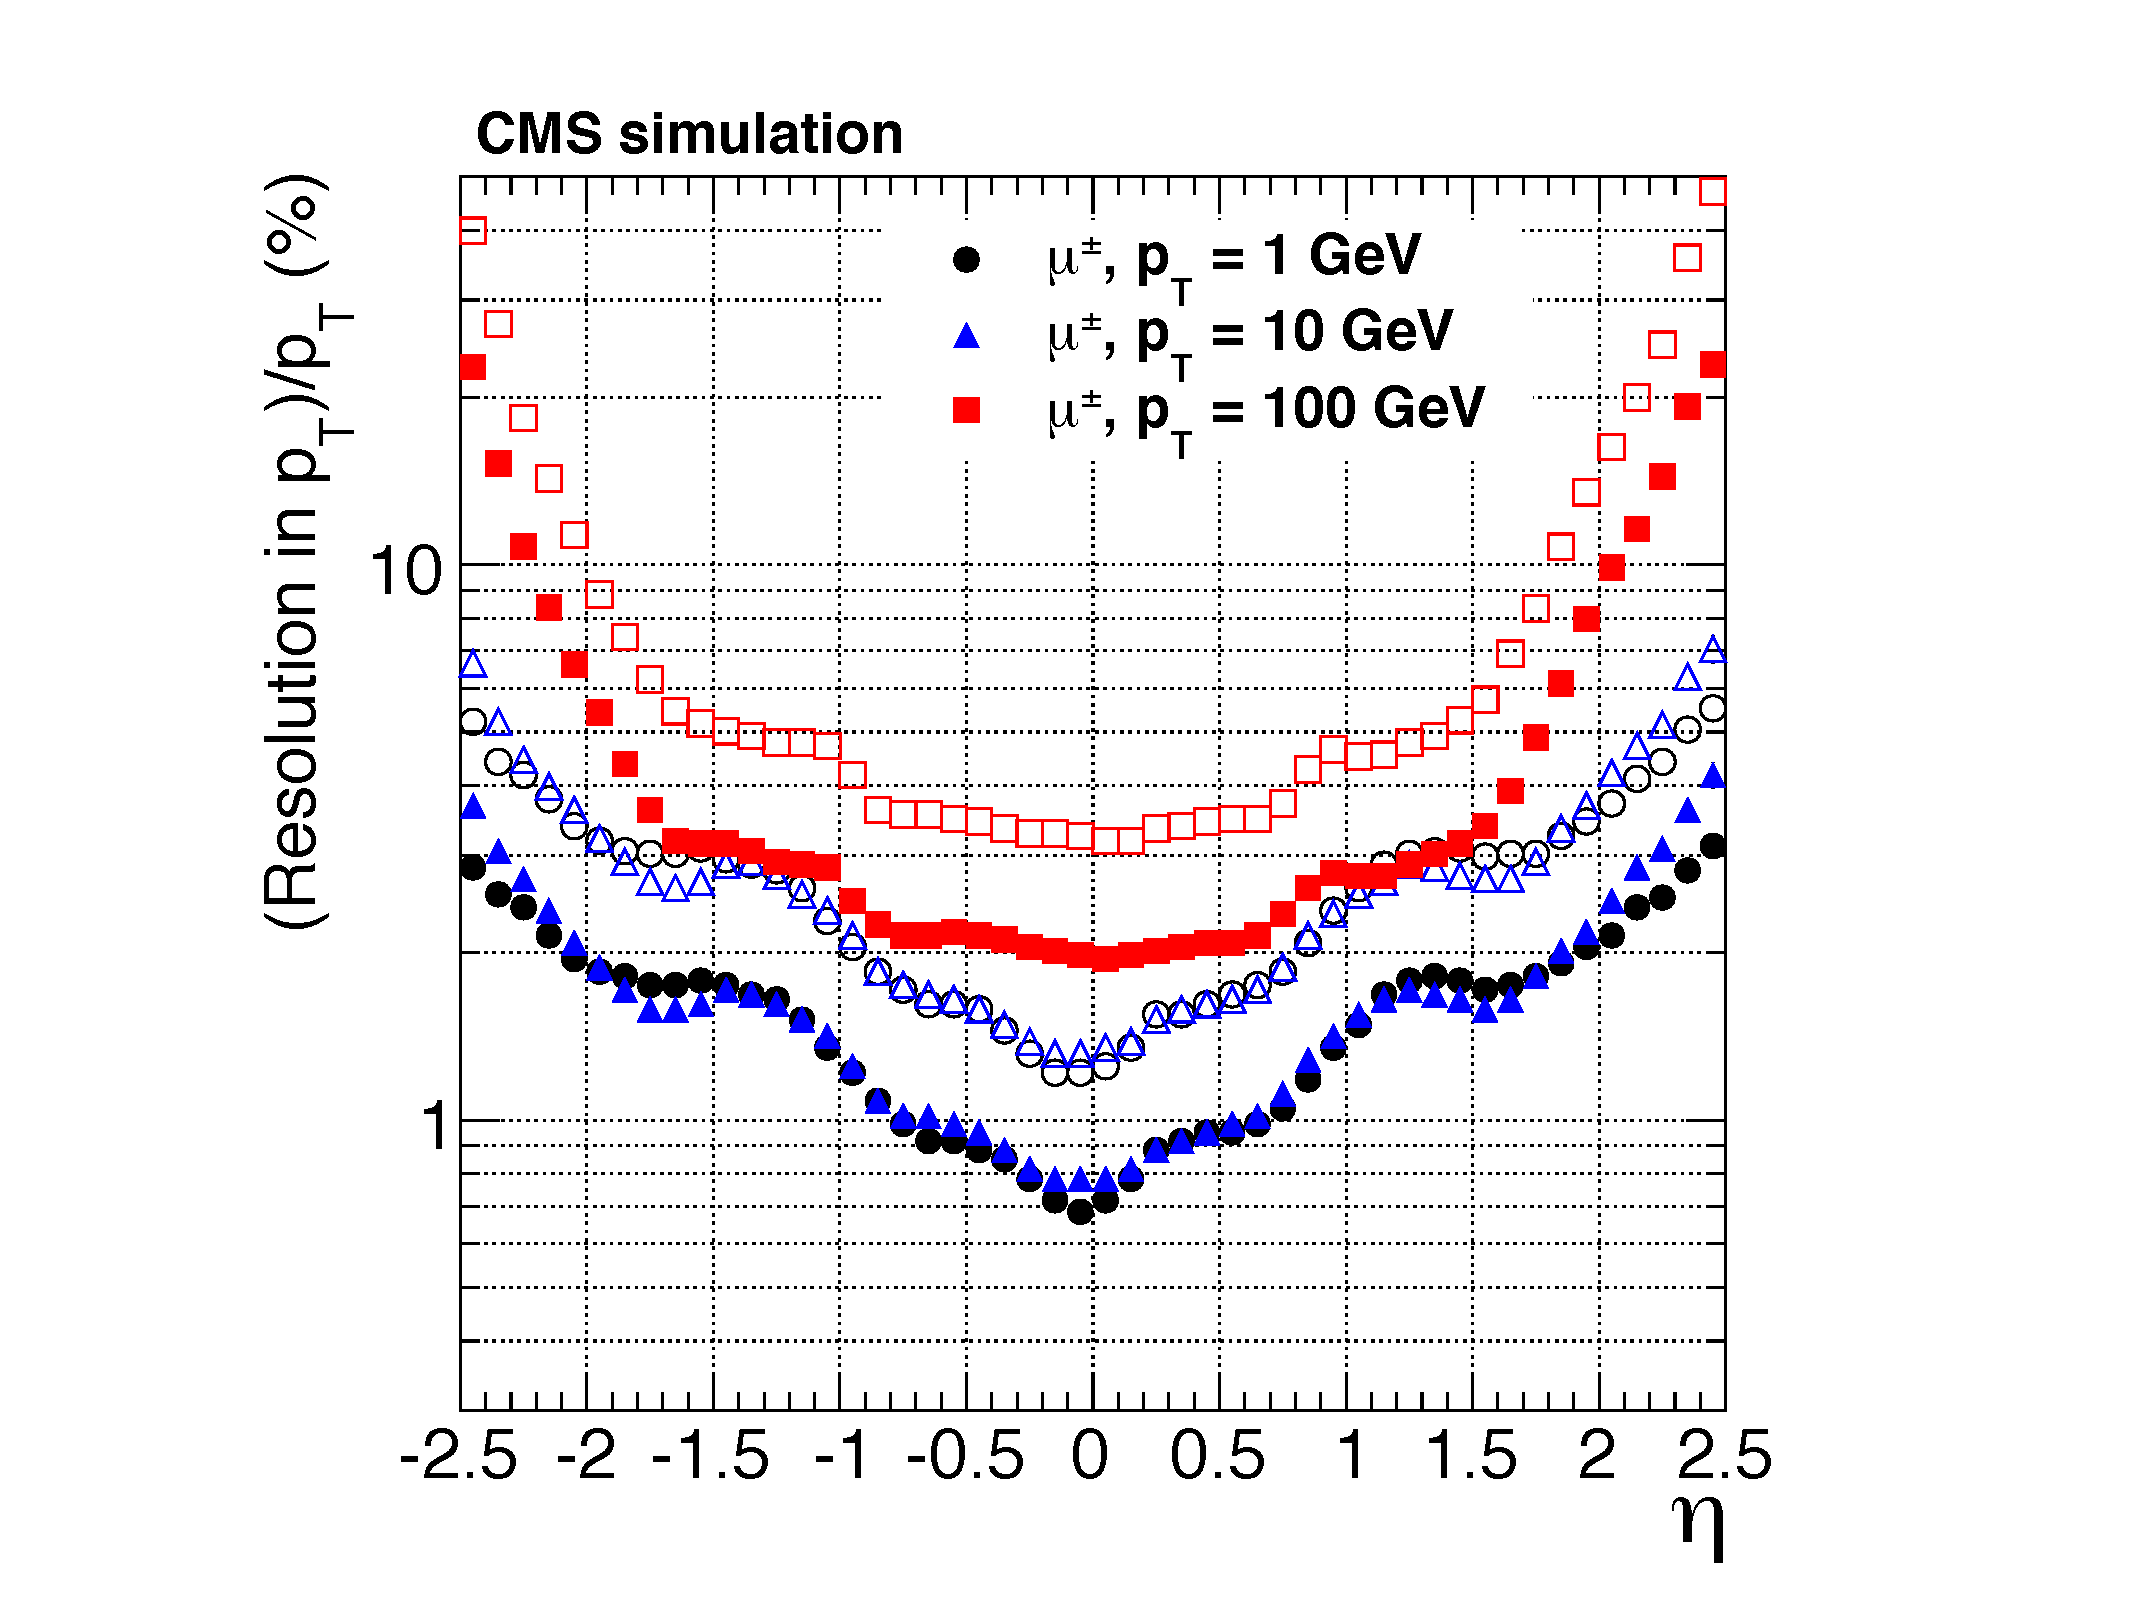
\includegraphics[width=0.49\textwidth]{CMS_DetectorFigures/TrackerPtResolution.pdf}
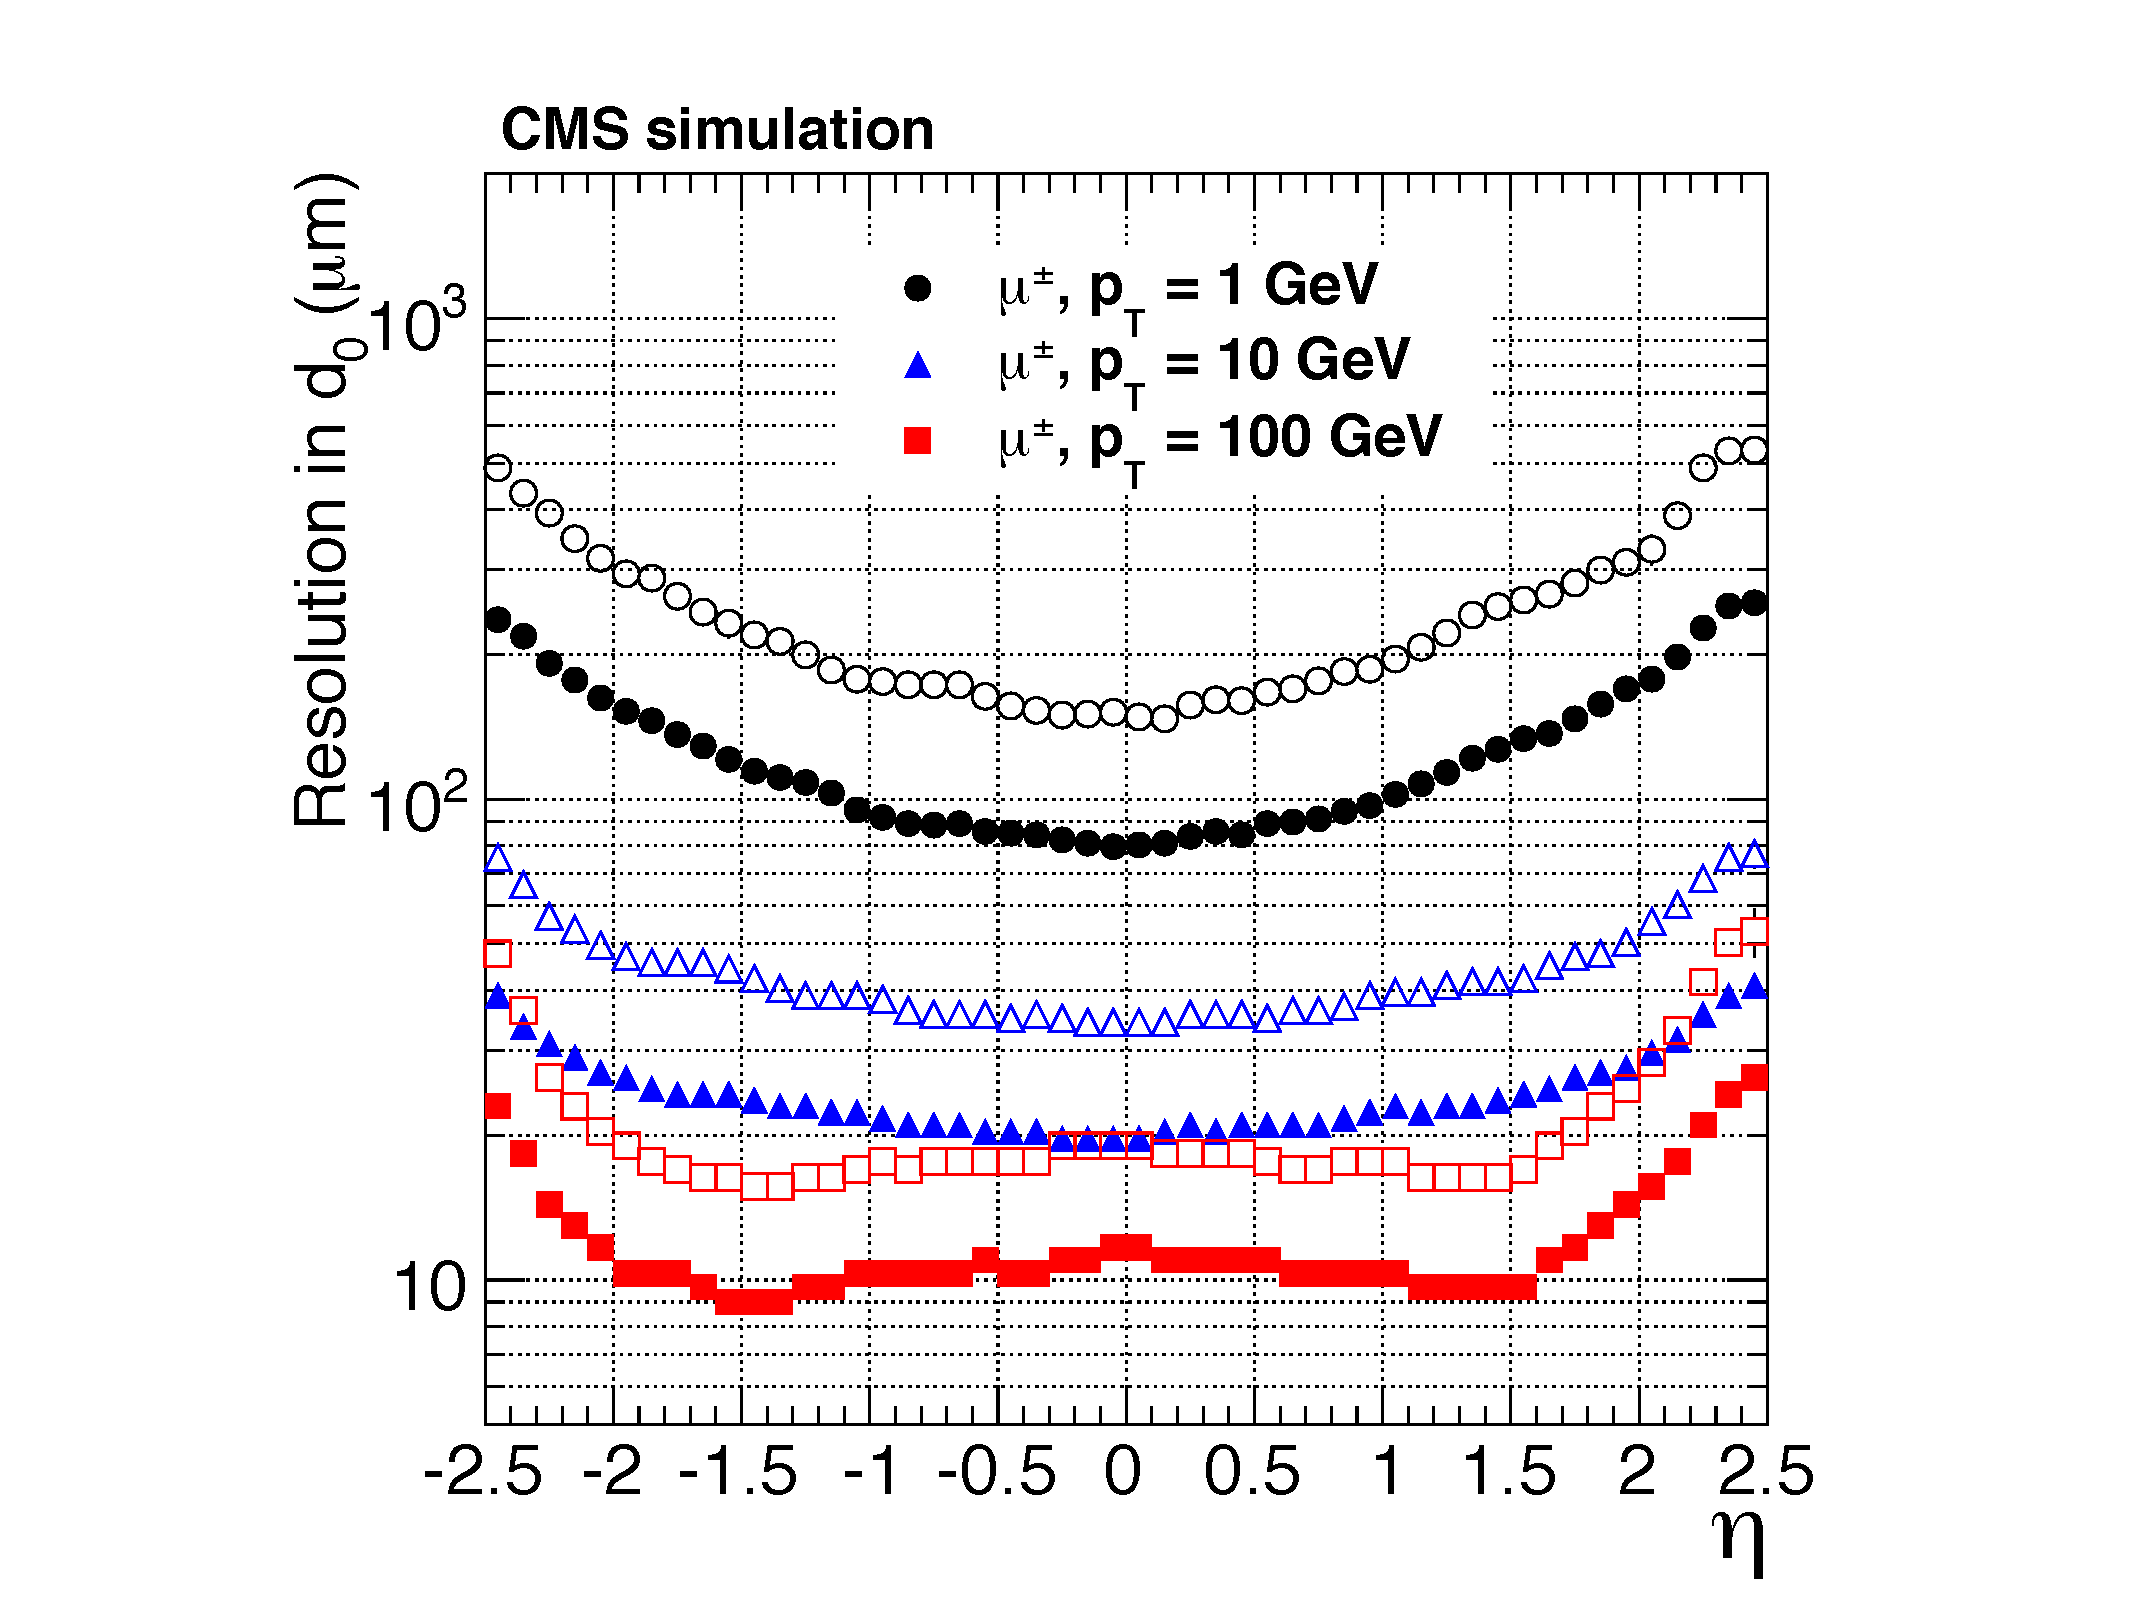
\includegraphics[width=0.49\textwidth]{CMS_DetectorFigures/TrackerImpactParameterResolution.pdf}
 \caption{Resolution as a function of the pseudorapidity $\eta$ for
   muons of $p_{\mathrm{T}} = $ 1, 10, and 100\GeV. The left panel
   shows the trasverse momentum resolution and the right panel the
   transverse impact parameter resolution. Both quantities are
   estimated from Simulation.\label{fig:MuonResolution}}
\end{figure}



\section{The Electromagnetic Calorimeter}
The CMS electromagnectic calorimeter (ECAL) is a granular and homogeneous
calorimeted built out of 61,200 lead tungstate (PbWO$_{4}$) crystals
in the barrel and closed by 7,324 PbWO$_{4}$ crystals in each of the
two endcaps. Additionally, a preshower detector is place in front of
the endcaps -- i.e. closer to the interaction point. The scintillating
light is collected by silicon avalanche photodiodes (APDs) in the ECAL barrel
(EB) and by vacuum phototriodes (VPTs) in the ECAL endcaps
(EE). Figure~\ref{fig:ECALgeometry} shows a projectional schematic
layout as well as a geometric view of a quarter of the CMS ECAL. The
ECAL excellent performance is one of the keystones of the physics
results of the CMS experiment, perhaps, best exemplyfied by the Higgs
boson search and characterization in the H$\rightarrow\gamma\gamma$
and H$\rightarrow$ZZ$^{*}$ decay channels~\cite{CMSHgg, CMSHzz}.

\begin{figure}
 \centering
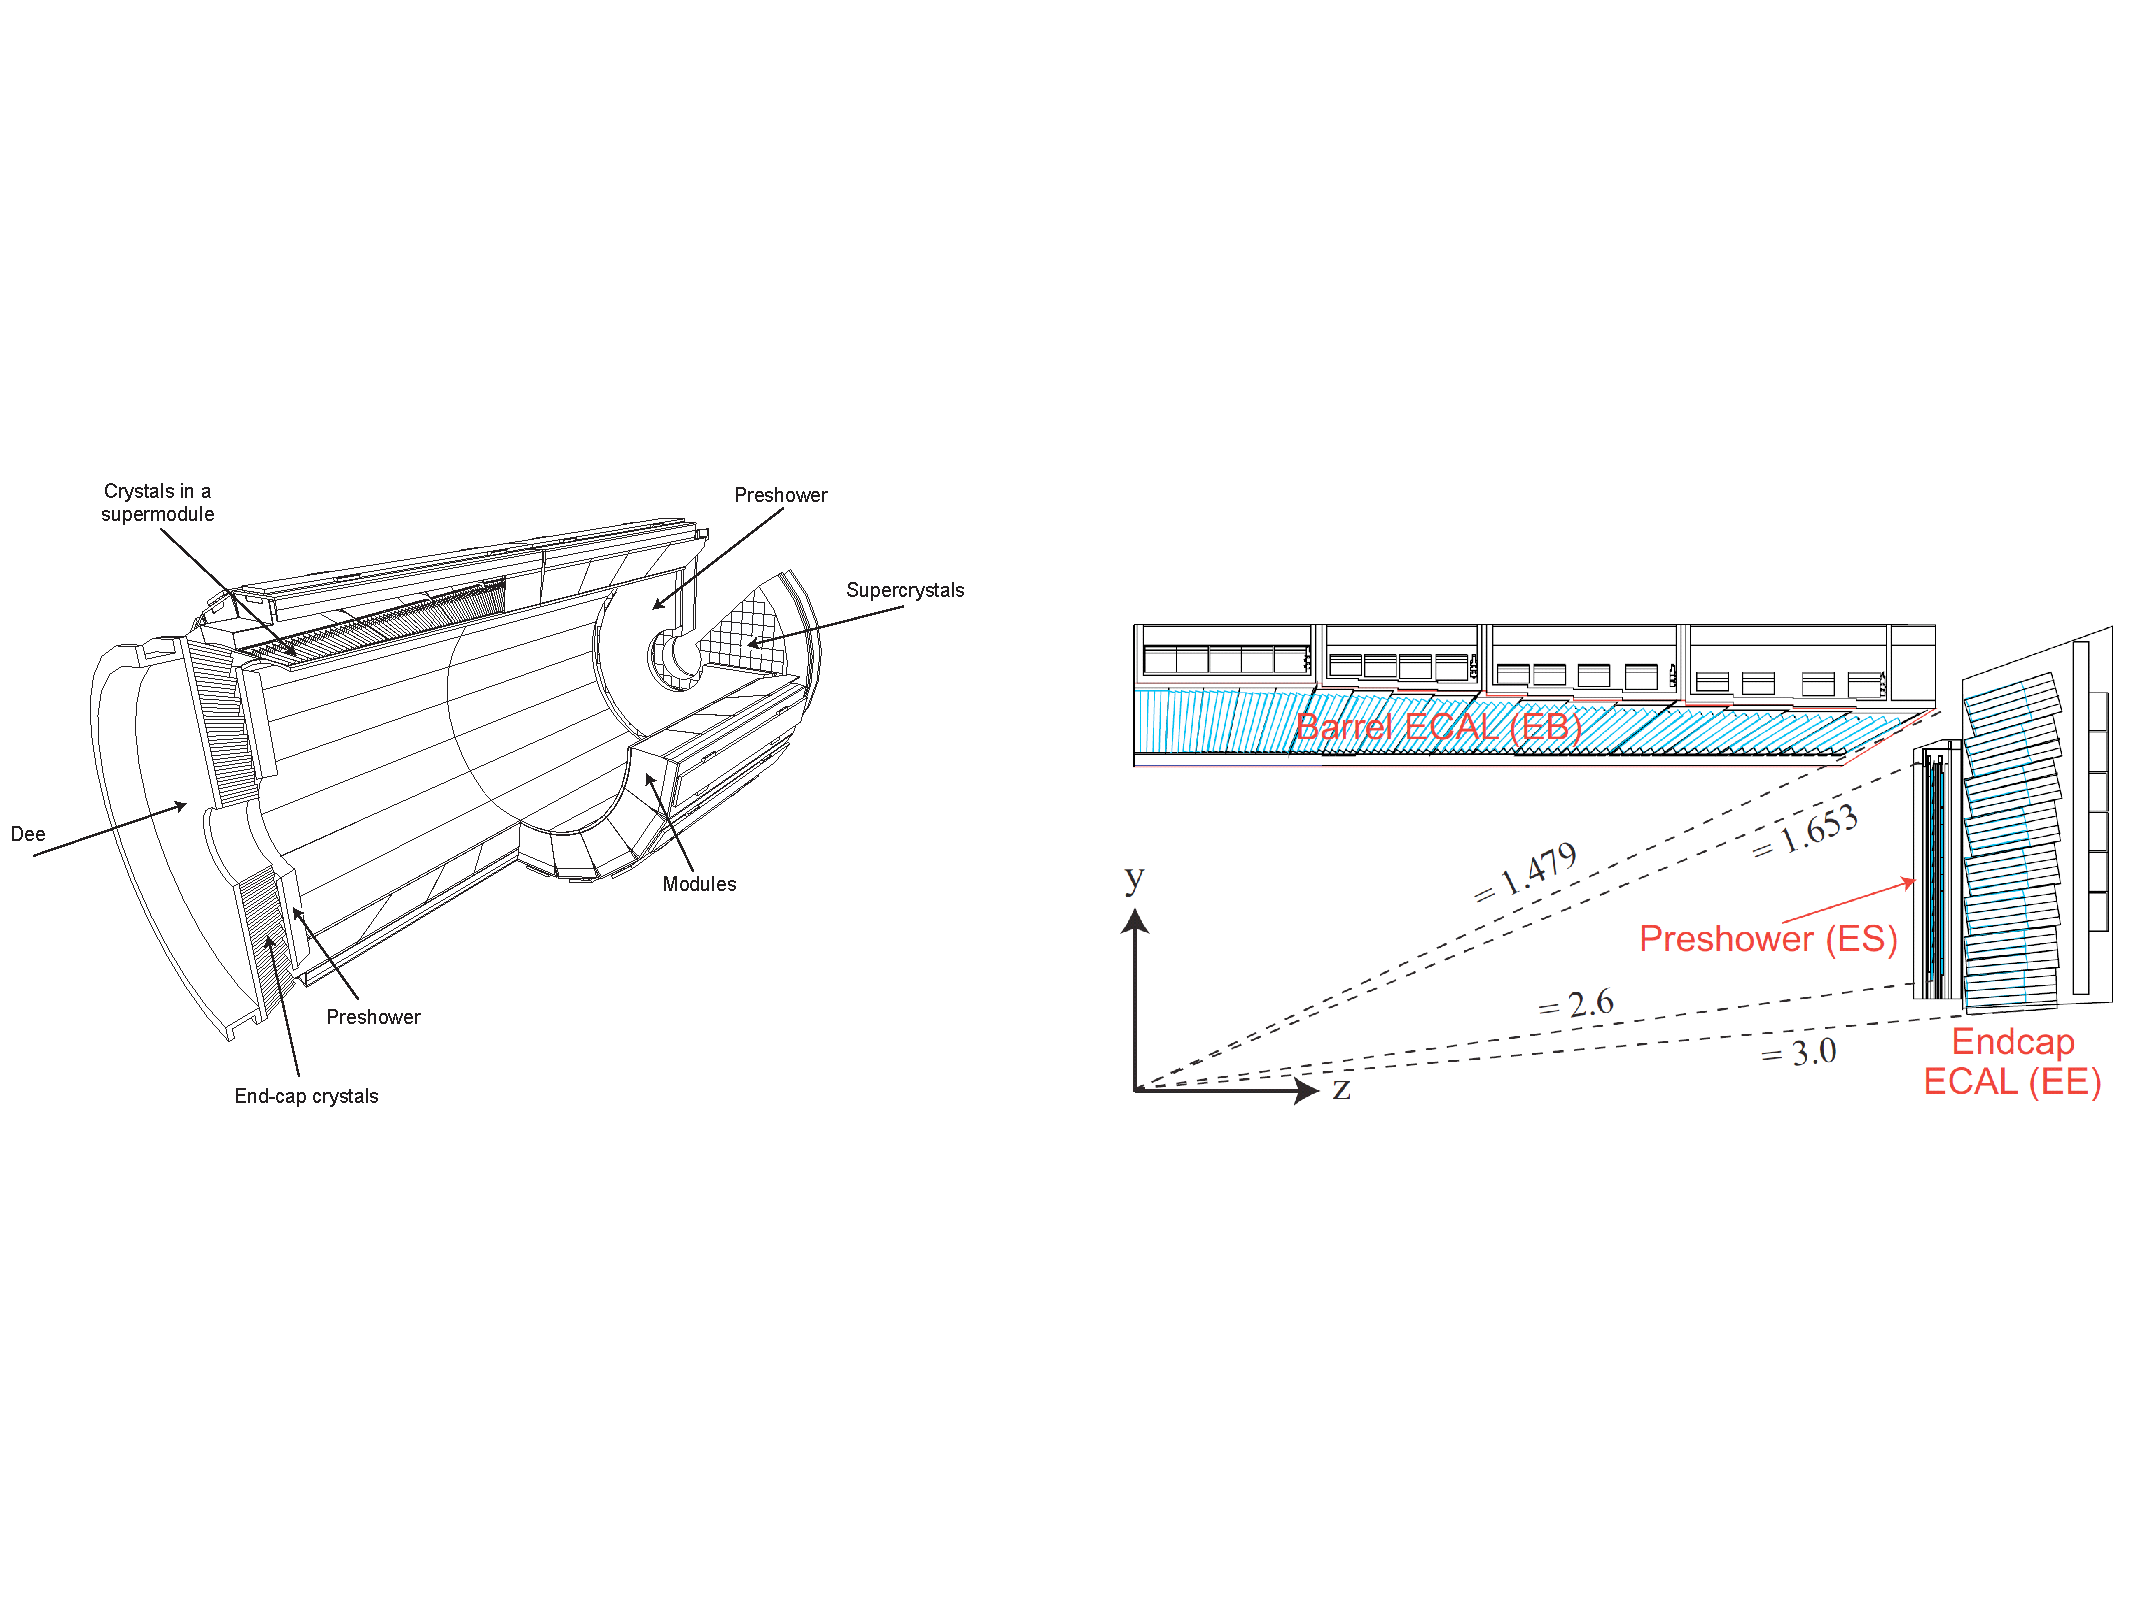
\includegraphics[width=0.99\textwidth]{CMS_DetectorFigures/ECAL_Geometry.pdf}
\caption{The layout of the CMS electromagnetic calorimenter. The left
  panel shows a projectional schematic
layout including all the major parts while the left panel shows a
geometric view of a quarter of the ECAL.\label{fig:ECALgeometry}}
\end{figure}

The PbWO$_{4}$ crystals with a density of 8.28 g/cm$^{3}$ provided a
good candidate because of its small radiation length ($X_{0} = 0.89$
cm), small moli\`ere radious (2.19 cm), and fast response. PbWO$_{4}$
crystals have a relatively low light yield of about 10
photo-electrons/MeV and therefore they required to be read out by
sensors with internal amplification inside the 3.8 T magnetic
field. The crystals in the EB are 23 cm long and have a
cross-sectional area of 2.2$\times$2.2 cm$^{2}$ (equivalent to
0.0174$\times$0.0174 in $\eta$, $\phi$), they are located at radious
of 1.29 m and arranged
in a quasi-projective geometry with 170 crystals -- 85 at each side --  covering up to a pseudorapidity range
$|\eta| < 1.48$. With 360 crytals in the $\phi$  direction the EB is
fully hermetic. The EE crystals are located at $z = \pm$ 315.4 cm, they
have a cross-sectional are of 2.86$\times$2.86 cm$^{2}$  and
3.0$\times$3.0 cm$^{2}$ at the front an rear faces, respectively, and
a length of 22 cm. They crystals are grouped in mechanical structure
of 5$\times$5 crystals and arranged in the traditional $x$-$y$
directions. Each endcap is divided into halves or \textit{Dees},
holding 3,662 crystals. The EE extends the ECAL coverage up to the
range $1.479 < |\eta| < 3.0$. The left and right panels of
Figure~\ref{fig:ECALcrystals} show the EB crystal instrumented with an
APD ant the EE crystal instrumented with a VPT, respectively.  Real
photographs of an EB module equipped with crystal is presented in
Figure~\ref{fig:ECALEB_module} while an EE Dee fully instrumented with crystals is shown
in Figure~\ref{fig:ECALEE_module}.
\begin{figure}
 \centering
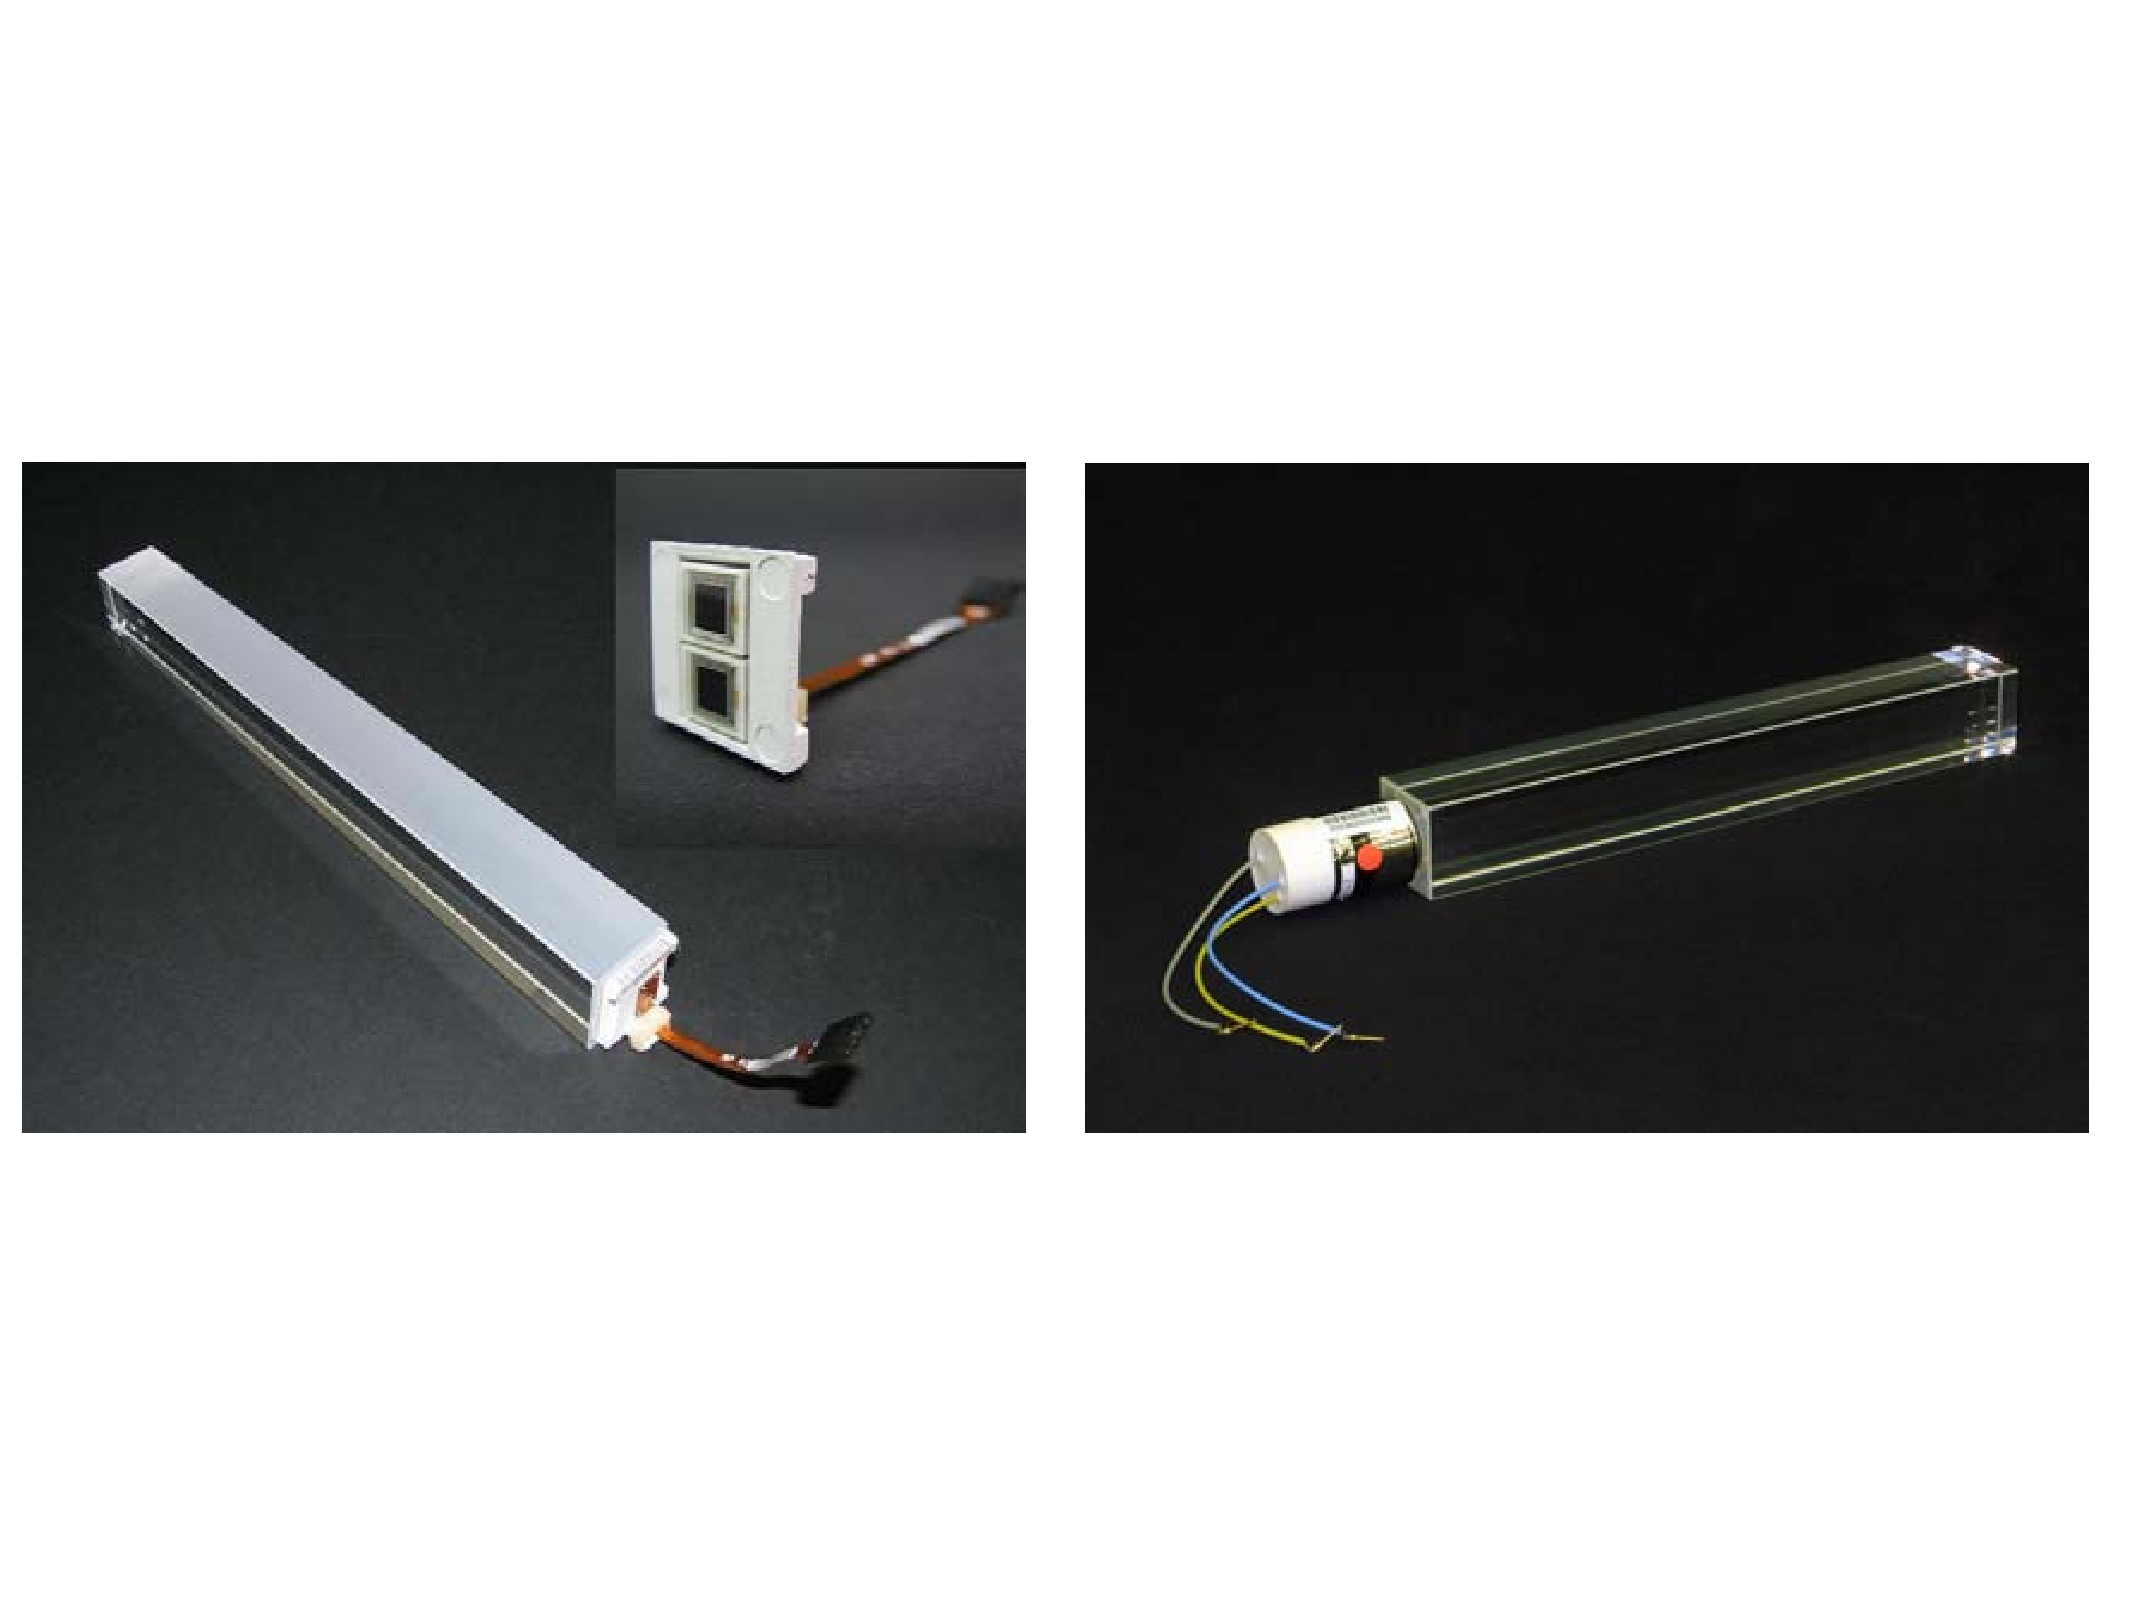
\includegraphics[width=0.99\textwidth]{CMS_DetectorFigures/EcalCrytals.pdf}
\caption{The  PbWO$_{4}$ crystal of the CMS ECAL, (left) a EB crystal
  instrumented with an APD and (right) a EE crystal instrumented with a VPT.\label{fig:ECALcrystals}}
\end{figure}
\begin{figure}
 \centering
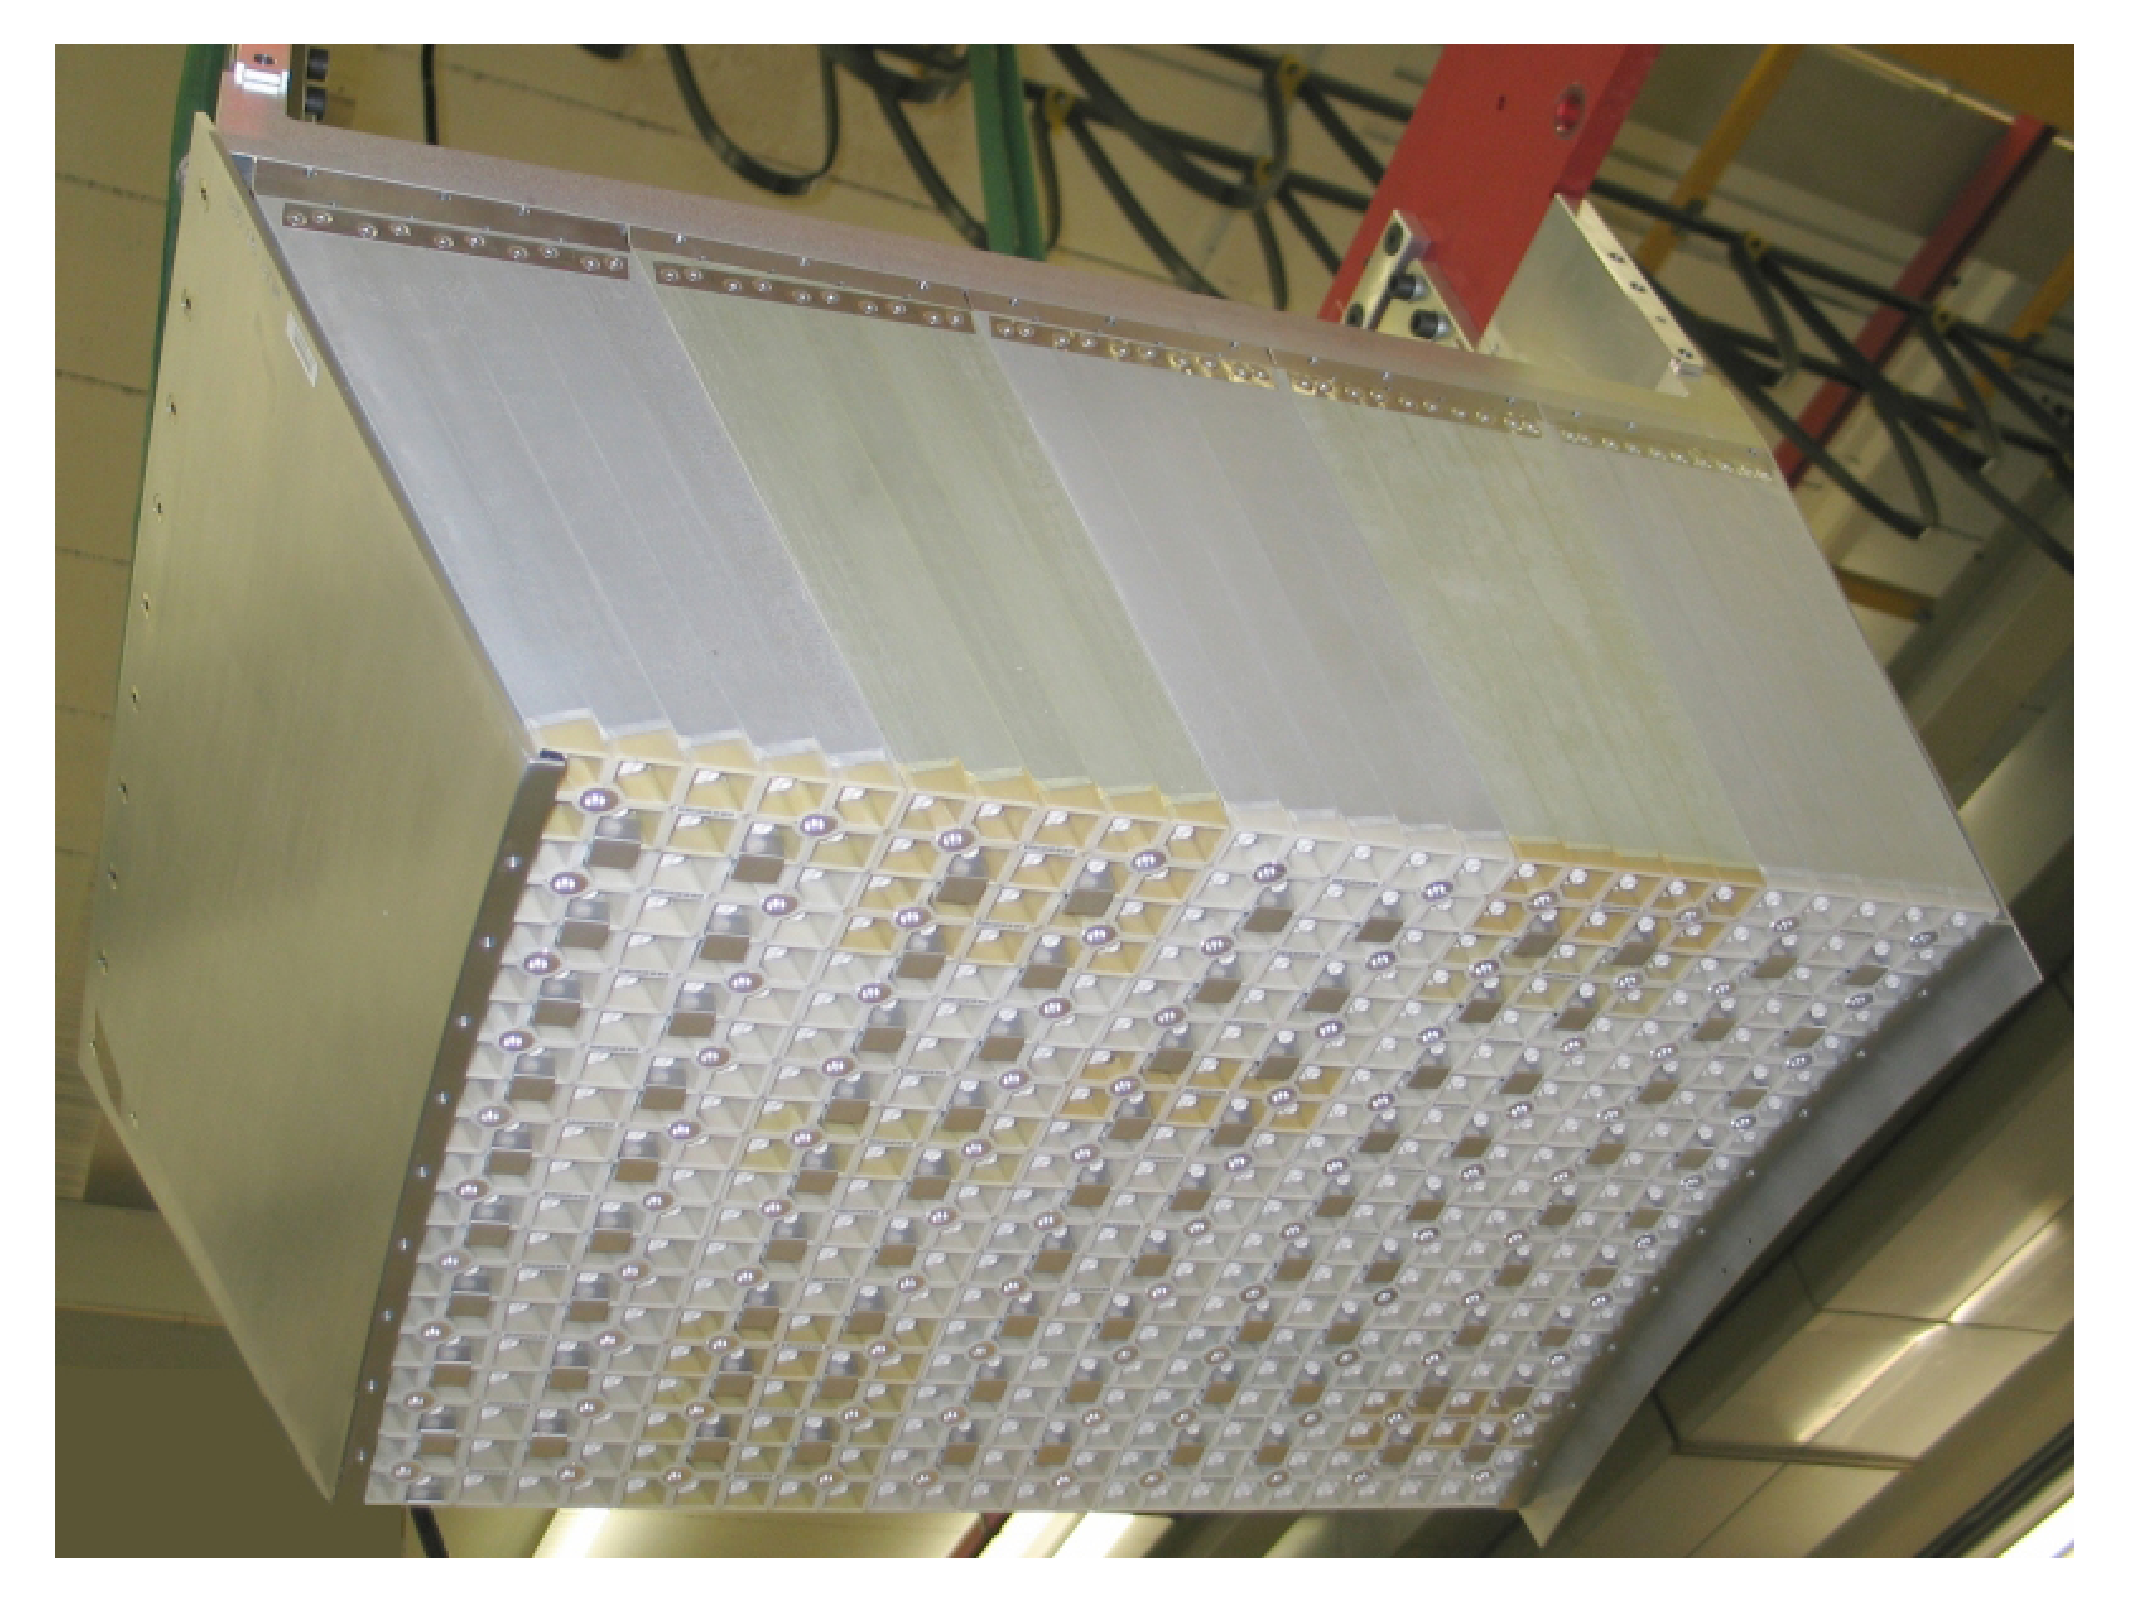
\includegraphics[width=0.99\textwidth]{CMS_DetectorFigures/ECALEB_Module.pdf}
\caption{A photograph of a EB module instrumented with crystals.\label{fig:ECALEB_module}}
\end{figure}
\begin{figure}
 \centering
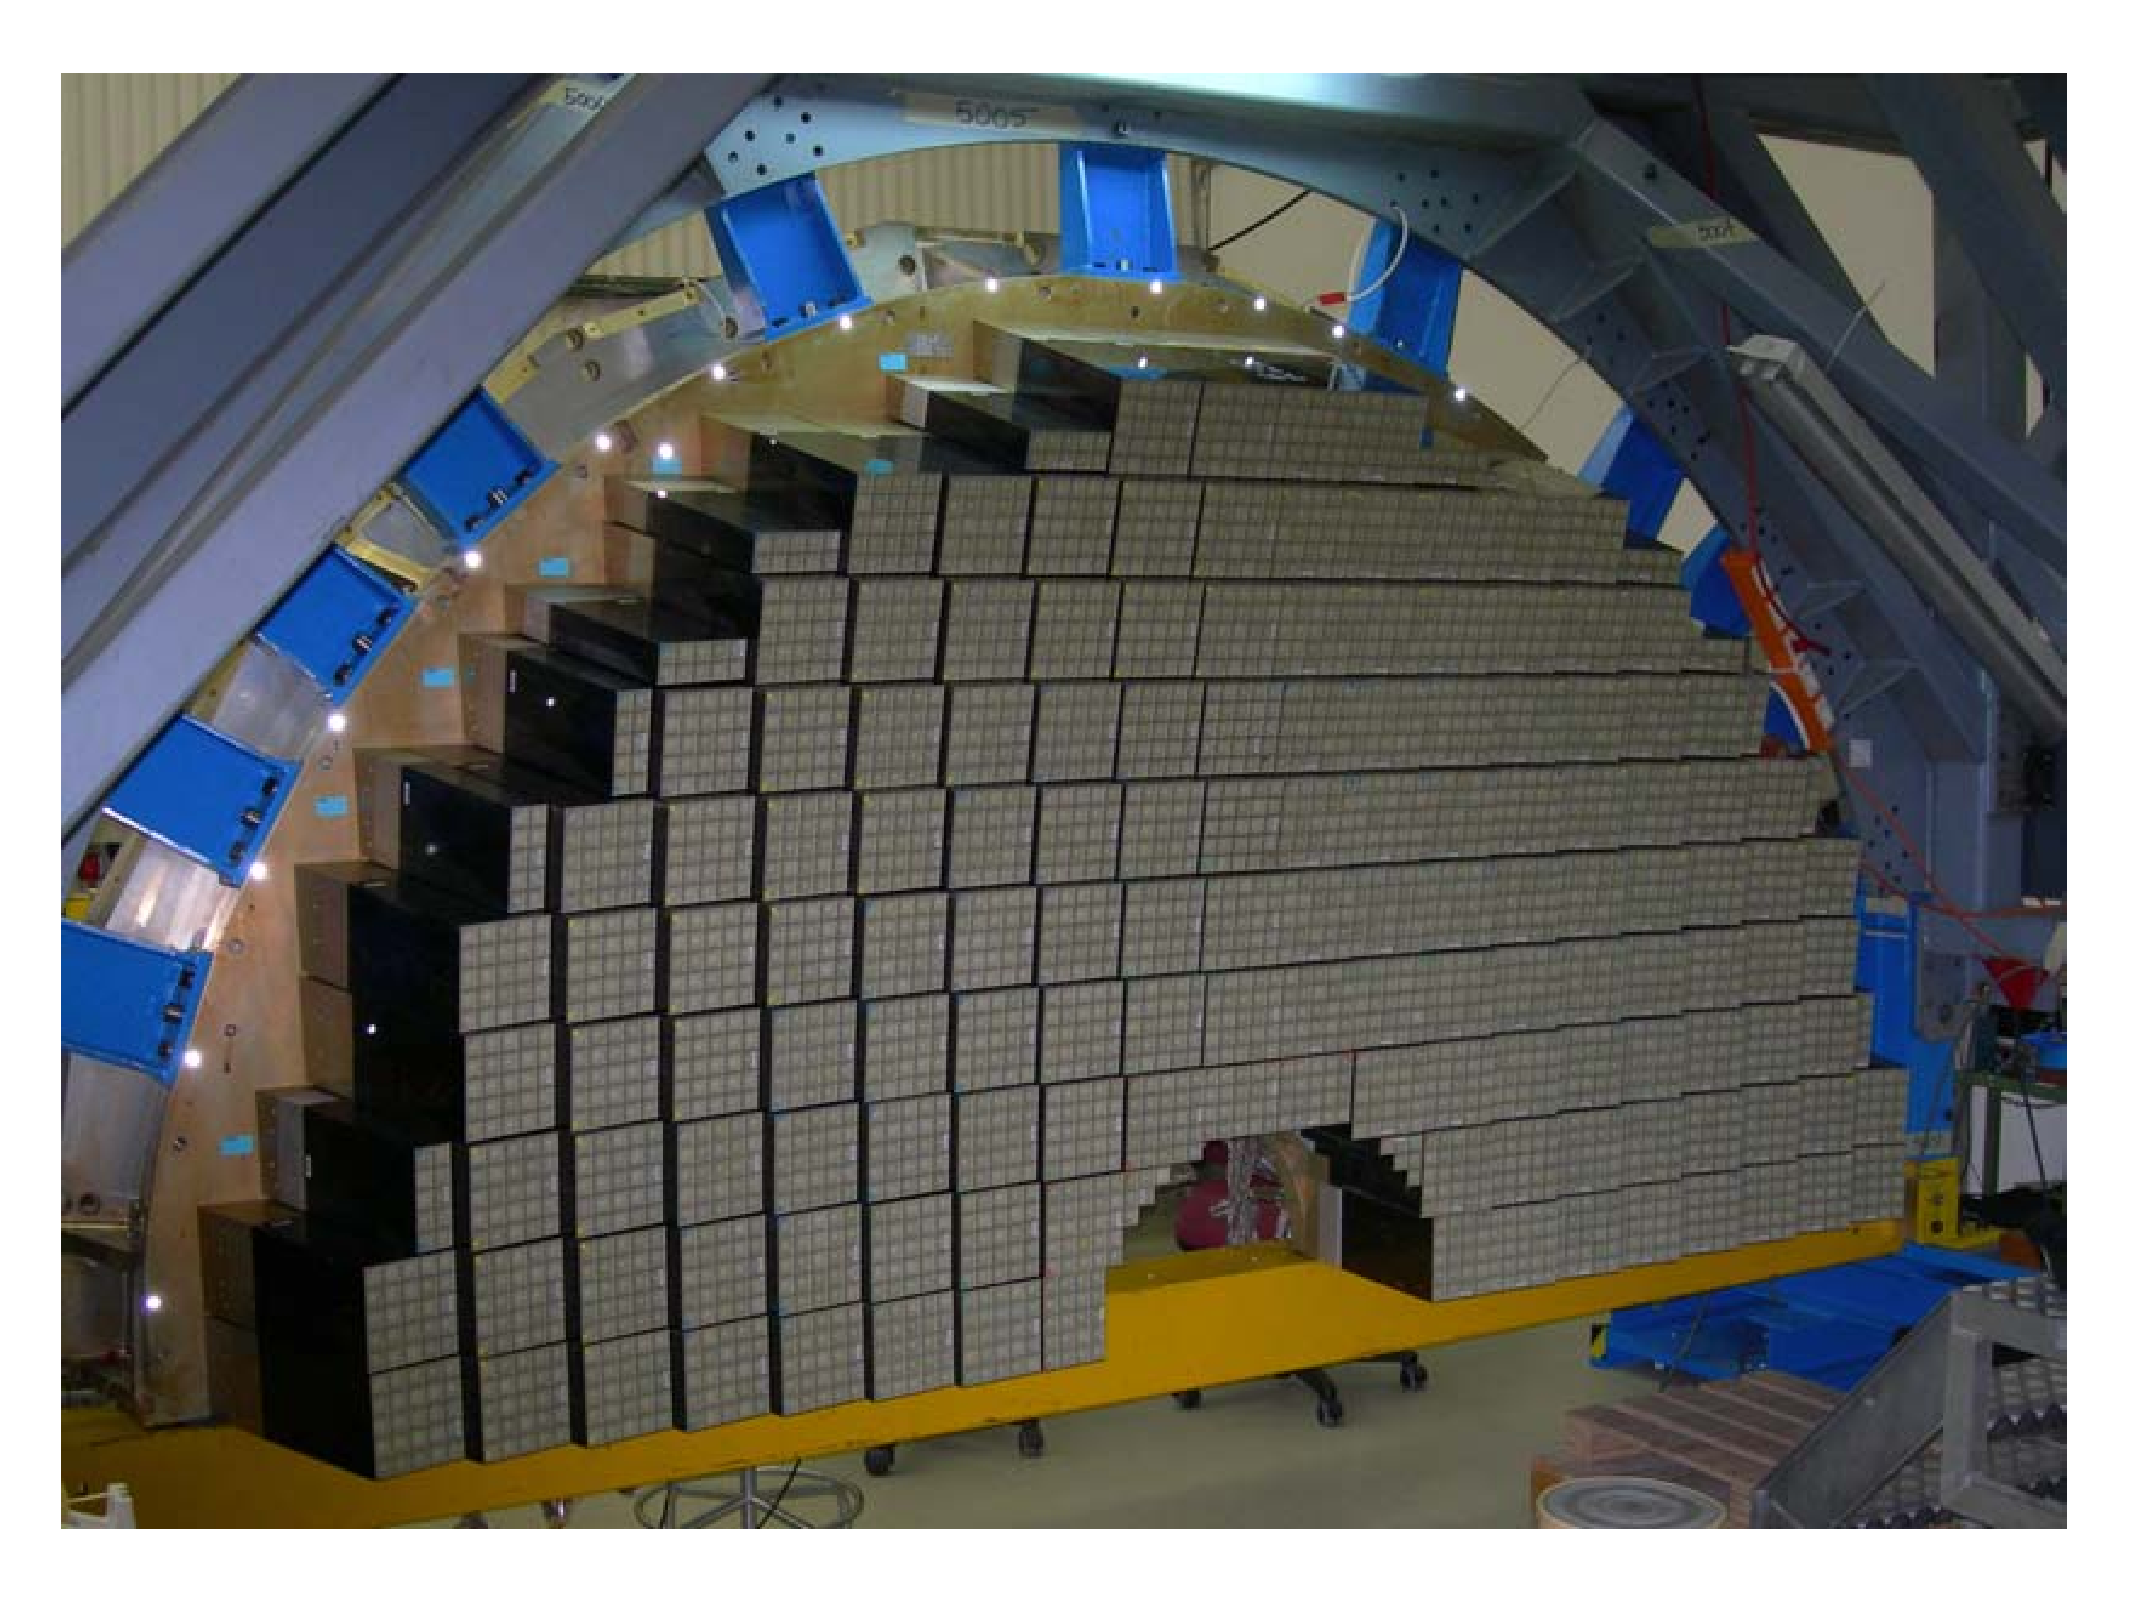
\includegraphics[width=0.99\textwidth]{CMS_DetectorFigures/ECALEE_Module.pdf}
\caption{A photograph of a EE Dee instrumented with crystals.\label{fig:ECALEE_module}}
\end{figure}
\subsection{ECAL Perfomance}

The EB has been extensively tested using electron beams, in this test
beam setup -- with no magnetic field or material in front -- the
energy resolution has been measured to be:
\begin{equation}\label{eq:ecalRes}
\frac{\sigma_{E}}{E} = \frac{2.8\%}{\sqrt{E(\GeV)}} \oplus
\frac{12\%}{E(\GeV)} \oplus 0.3\%,
\end{equation}

where E is the electron beam energy in units of \GeV. The terms in the
right-hand side of the Eq.~\ref{eq:ecalRes} are the so called
stochastic, noise, and constant terms. The first is due to the
fluctuations related to the development of the electromagnetic shower
inside the calorimenter crystals, the second is dues to electronic
noise of the readout chain, and the last is related to the
instrumental effect such as non-linear response, radiation damage,
shower leakage among others.

The test beam ideal conditions clearly differ from those at the CMS
experiment and therefore in situ measurements of the performance of
the ECAL have been performed durin the data-taking period at 7 and
8\TeV. One key measurement is the trigger efficiency for
electron/photon (e/$\gamma$) candidates, the Level-1 trigger was
operated with a threshold of $E_{T}$ = 20\GeV (provided by 5$\times$5
crystals) in 2012 and found to be above 99\% efficienct for $E_{T}$ >
40\GeV, thus enabling a fully efficienct H$\rightarrow\gamma\gamma$
search.

The e/$\gamma$ energy measurement depends upon the correct
reconstruction of electromagnetic showers in the ECAL. Some e/$\gamma$
candidates interact -- by bremsstrahlung or photon conversion -- with
the silicon tracker  prior reaching the ECAL or their trajectories are
modified due to the 3.8 T magnetic field causing the showers to spread
on the azhimutal direction and thus their energy is shared by multiple
crystals. In order to account for these effect and ensure a more
accurate e/$\gamma$ reconstruction a dynamic clustering algorithim is
used to merge clusters of energy deposited that belong to the same
electromagnetic shower into the so-called \textit{superclusters}
(SCs). Once the SC is formed, the e/$\gamma$ candidate energy
($E_{e/\gamma}$) is reconstructed using the following expression:

\begin{equation}
\label{eq:ecalE}
E_{e/\gamma} = F_{e/\gamma}\cdot \big(G\cdot\sum S_{i}(t)C_{i}A_{i} + E_{\mathrm{ES}}\big)
\end{equation}
 
where $F_{e/\gamma}$ is a correction accounting for the imperfect
clustering, material, and geometric efffect; $G$ is the ADC-to-\GeV
conversion; $S_{i}(t)$ is the time-dependent correction to account for
the response variations of the $i$-th crystal; $C_{i}$ is the
inter-calibration coefficient of the $i$-th crystal; $A_{i}$ is the
amplitude of the $i$-th crystal in ADC counts; finally,
$E_{\mathrm{ES}}$ is the pre-shower energy -- only relevant for
e/$\gamma$s in the EE. Figure~\ref{fig:ECAL_clusterE} shows the effect
of the clustering process and the application of the $F_{e/\gamma}$
correction by comparing the invariant mass of $e^{+}e^{-}$ pairs
coming from a Z boson with respect to the usage of the simple fixed
5$\times$5 cluster energy.

\begin{figure}
 \centering
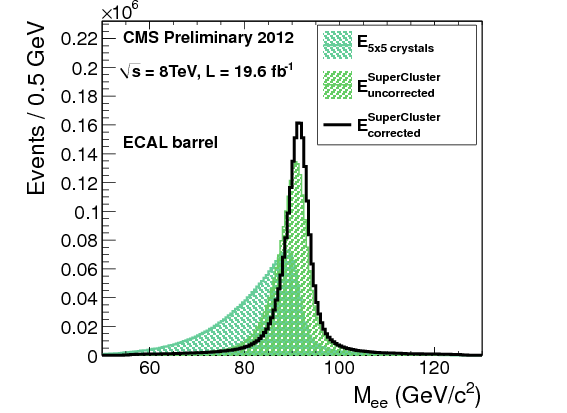
\includegraphics[width=0.49\textwidth]{CMS_DetectorFigures/E_corr-EB.png}
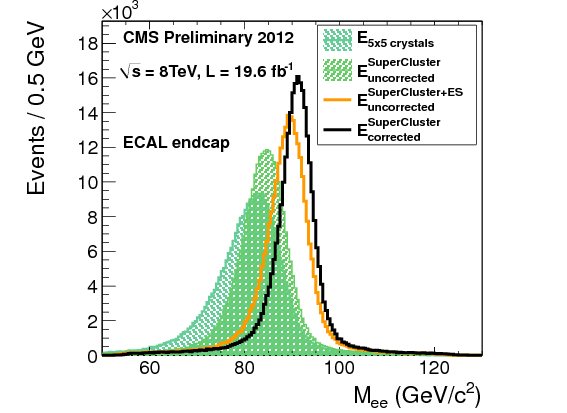
\includegraphics[width=0.49\textwidth]{CMS_DetectorFigures/E_corr-EE.png}
\caption{The reconstructed Z invariant mass from $e^{+}e^{-}$
  decays. The left and right panels show the reconstructed invariant mass for
  the EB and EE, repectively, with different algorithms to reconstructed electron energies.\label{fig:ECAL_clusterE}}
\end{figure}

The inter-calibration coefficient is responsible for correcting the
channel-to-channel variation in response. The main sources for such
variations are the crystal light yield variations ( up to $\sim$ 15\%)
and the spread on the gain of the photodetectors ( up to $\sim$
25\%). An inter-calibration is carrried out in situ by methods that
explote the time- and $\phi$-invariance of the energy flow in the
crystals at a given $\eta$ in minimum-bias events, as well as the
$\pi^{0}/eta$ mass constraint to the photons pair from its decay, and
the momentum constraint of isolated electrons from W and Z boson
decays. The precision of these methods as a function of $\eta$ is
shown in Figure~\ref{fig:ECAL_ICPrecision}. The invariant mass of
diphotons consistent with a $\pi^{0}$ and $\eta$ used in the
inter-calibration is shown in the left and right panels of
Figure~\ref{fig:ECAL_pizero}, respectively.

\begin{figure}
 \centering
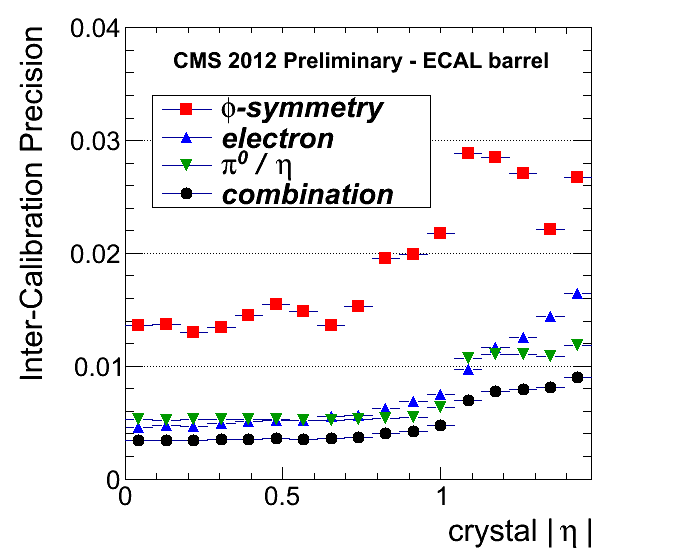
\includegraphics[width=0.49\textwidth]{CMS_DetectorFigures/2012EBprecWithCombV3.png}
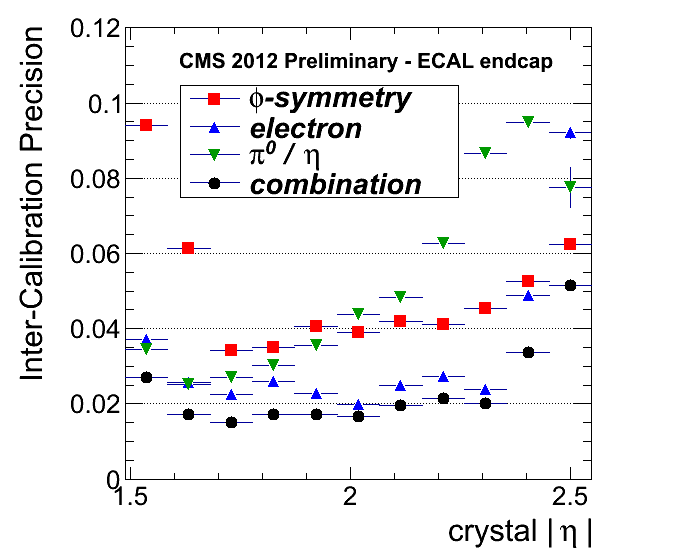
\includegraphics[width=0.49\textwidth]{CMS_DetectorFigures/2012EEprecWithCombV3.png}
\caption{The reconstructed Z invariant mass from $e^{+}e^{-}$
  decays. The left and right panels show the reconstructed invariant mass for
  the EB and EE, repectively, with different algorithms to reconstructed electron energies.\label{fig:ECAL_ICPrecision}}
\end{figure}

\begin{figure}
 \centering
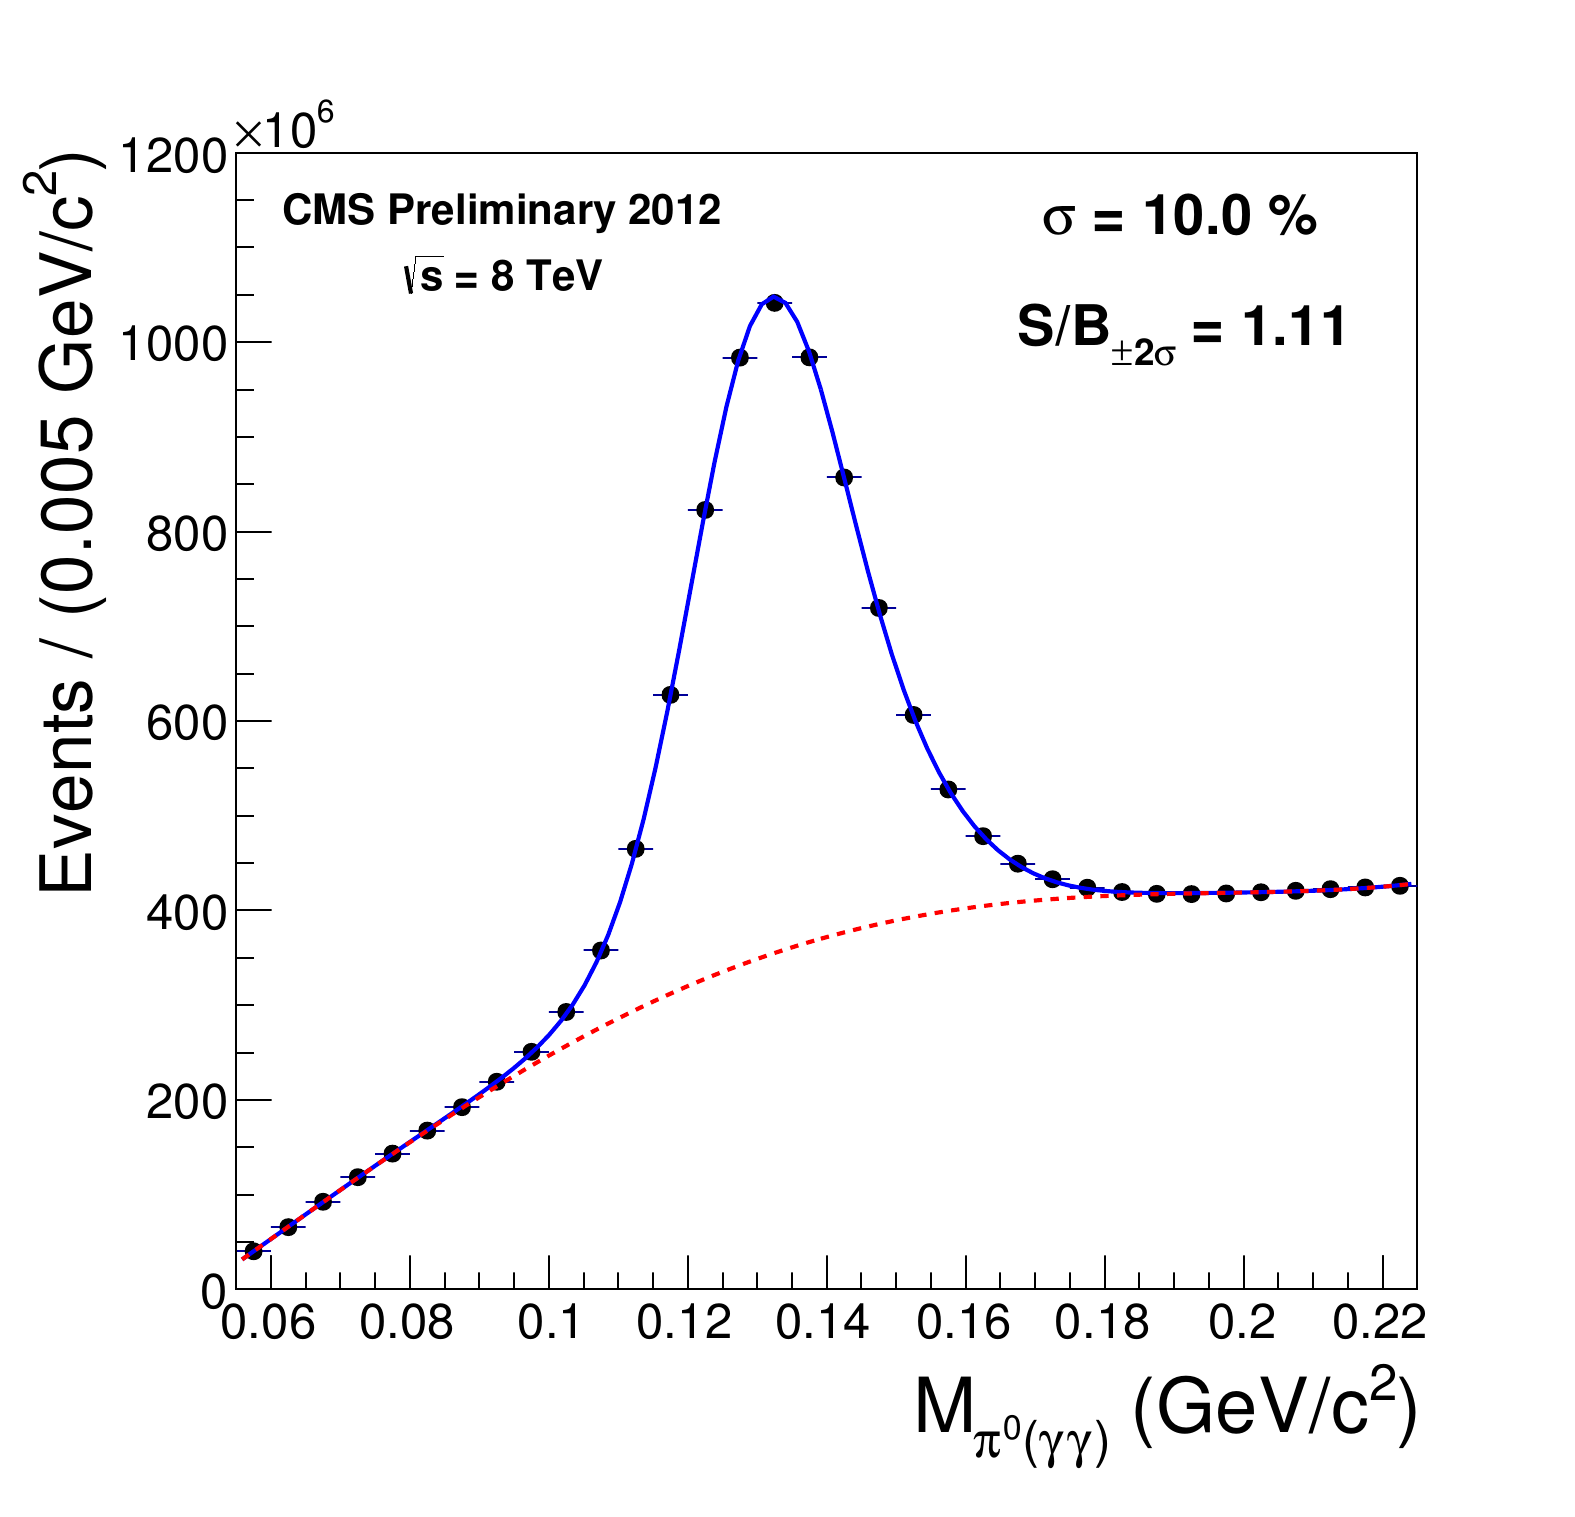
\includegraphics[width=0.49\textwidth]{CMS_DetectorFigures/EB_2012_pi0.png}
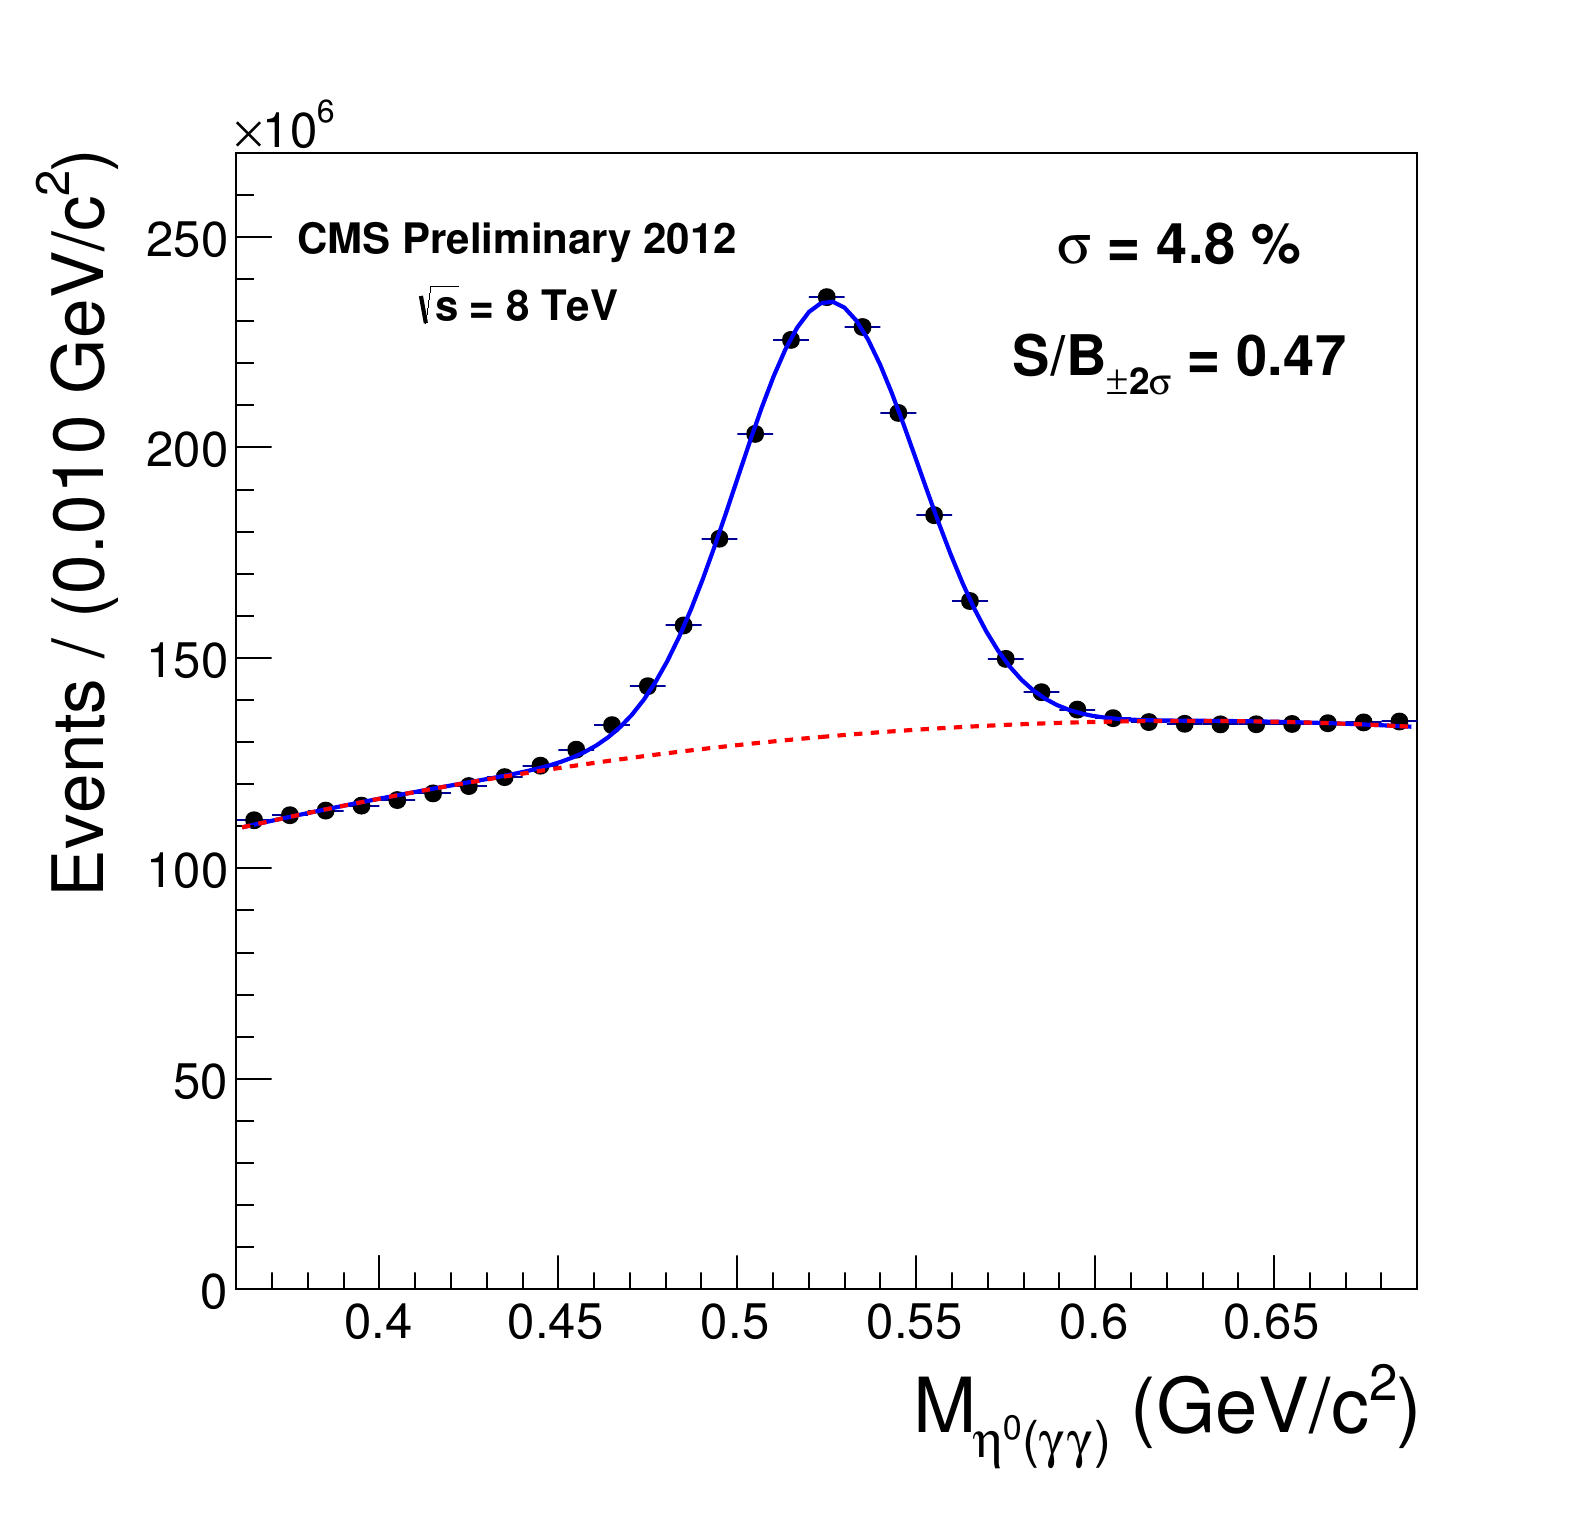
\includegraphics[width=0.49\textwidth]{CMS_DetectorFigures/EB_2012_eta0.png}
\caption{The reconstructed Z invariant mass from $e^{+}e^{-}$
  decays. The left and right panels show the reconstructed invariant mass for
  the EB and EE, repectively, with different algorithms to reconstructed electron energies.\label{fig:ECAL_pizero}}
\end{figure}
Another important ingredient to the precise measurement of the
electromagnetic shower energy is the time dependent corrections, at
CMS the ECAL crystals undergo changes in transparency due to the
radiation received while collisions occur, while  during downtime the
transparency is recovered. In order to correct for the transparency
changes a laser monitoring system is installed and run every $\sim$40
minutes. Laser light ($\lambda = 440$ nm) close to the emission peak of PbWO$_{4}$
is impinge into all the crystals, thus, tracking their response
variations. The variations on transparency as a function of time for
different $\eta$ ranges is shown in
the left panel of Figure~\ref{fig:ECAL_Transparency1}, where it is observed that the
transparency variations are more severe at large pseudorapidities. The
validity of the laser monitoring (LM) correction is checked using
electrons from W decays. The stability of the LM correction is
estimated by the rms of the $E/p$ ratio in these events and found to
be about 0.1\% and 0.3\% for the EB and EE, respectively. The right
panel of Figure~\ref{fig:ECAL_Transparency1} shown the LM correction
effect on electron from W events in the EE. The effect of the
inter-calibration and LM corrections is shown Figure~\ref{fig:ECAL_E_IC_LM}, where
the invariant mass of $e^{+}e^{-}$ pairs from Z decays is
reconstructed with and without such corrections being applied.
\begin{figure}
 \centering
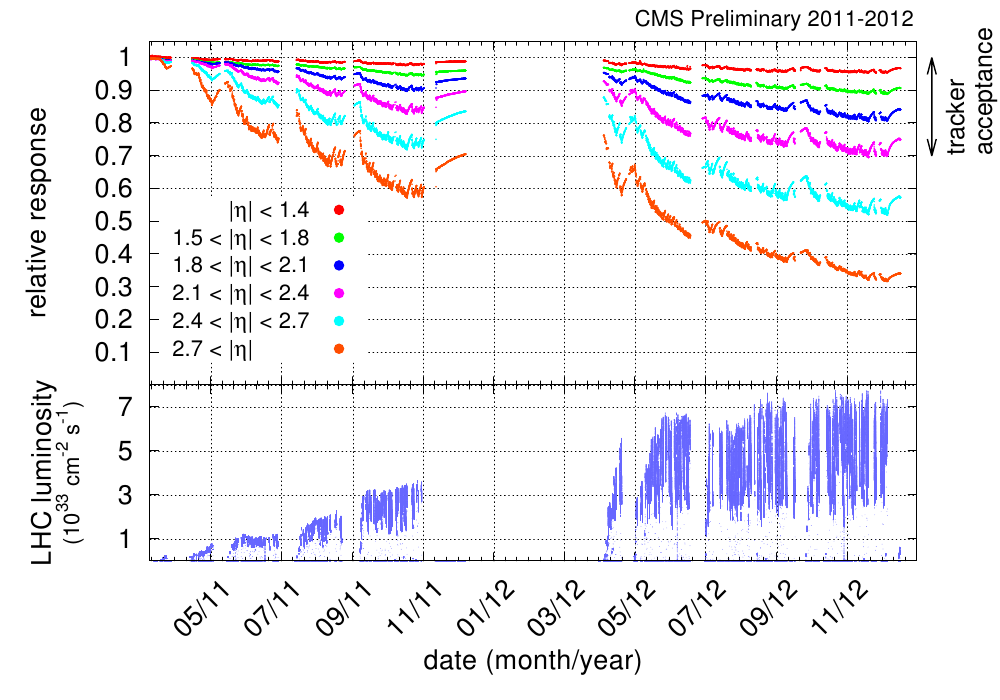
\includegraphics[width=0.99\textwidth]{CMS_DetectorFigures/histories_2011-2012.png}
\caption{The reconstructed Z invariant mass from $e^{+}e^{-}$
  decays. The left and right panels show the reconstructed invariant mass for
  the EB and EE, repectively, with different algorithms to reconstructed electron energies.\label{fig:ECAL_Transparency1}}
\end{figure}

\begin{figure}
 \centering
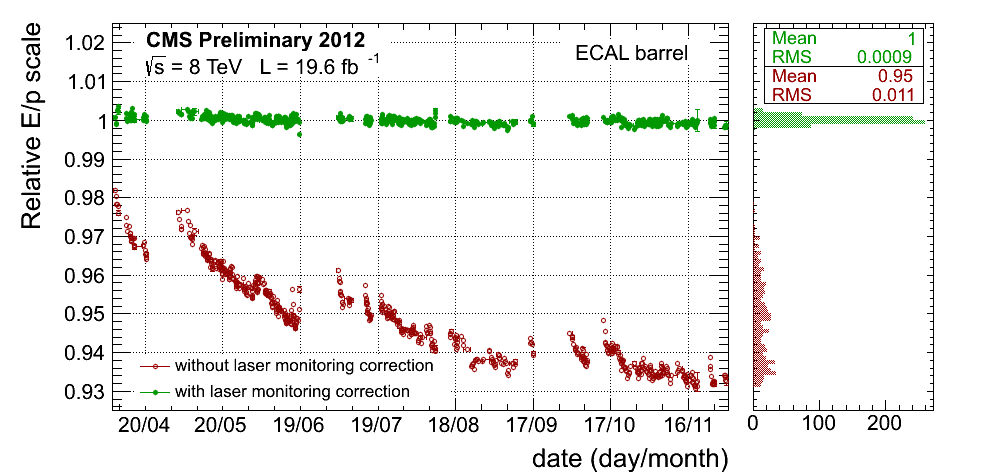
\includegraphics[width=0.99\textwidth]{CMS_DetectorFigures/approval_EB_Winter2013.png}
\caption{The reconstructed Z invariant mass from $e^{+}e^{-}$
  decays. The left and right panels show the reconstructed invariant mass for
  the EB and EE, repectively, with different algorithms to reconstructed electron energies.\label{fig:ECAL_response}}
\end{figure}

\begin{figure}
 \centering
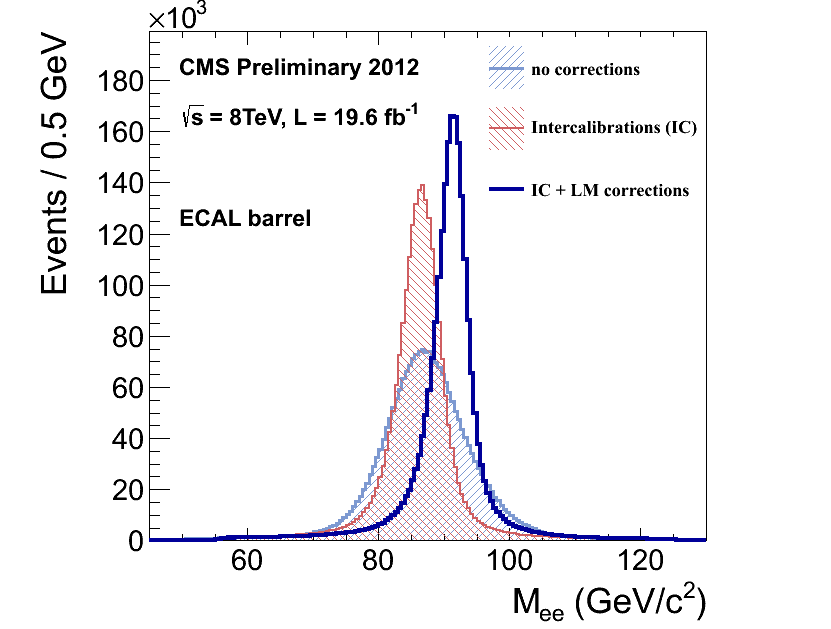
\includegraphics[width=0.49\textwidth]{CMS_DetectorFigures/noIC_noLaser-regrCorr_ele-EB.png}
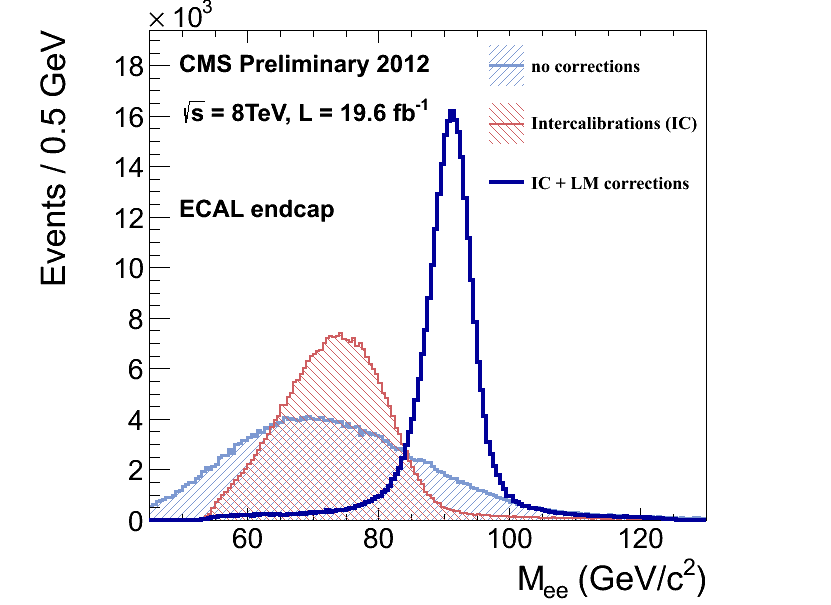
\includegraphics[width=0.49\textwidth]{CMS_DetectorFigures/propaganda_noIC_noLaser-regrCorr_ele-EE.png}
\caption{The reconstructed Z invariant mass from $e^{+}e^{-}$
  decays. The left and right panels show the reconstructed invariant mass for
  the EB and EE, repectively, with and without the IC and the LM corrections.\label{fig:ECAL_E_IC_LM}}
\end{figure}
 Finally, the overall energy resolution of the CMS ECAL has been measured
 and compared to simulation, this is shown in the right panel of
 Figure~\ref{fig:ECAL_Higgs}. The energy resolution is found to be
 between 1-2\% for $|\eta|<1$ and between 3-5\% in the EE, it is also
 observed that the simulation and measurement do not agree and that an
 extra constant term as a function of $\eta$ should be added to the
 simulation. The performance of the ECAL can also be observed in the
 width of the invariant mass of the Higgs boson, this is shown in the
 left panel of Figure~\ref{fig:ECAL_Higgs}, where a $\sigma_{eff}$ =
 1.36\GeV is observed.
\begin{figure}
 \centering
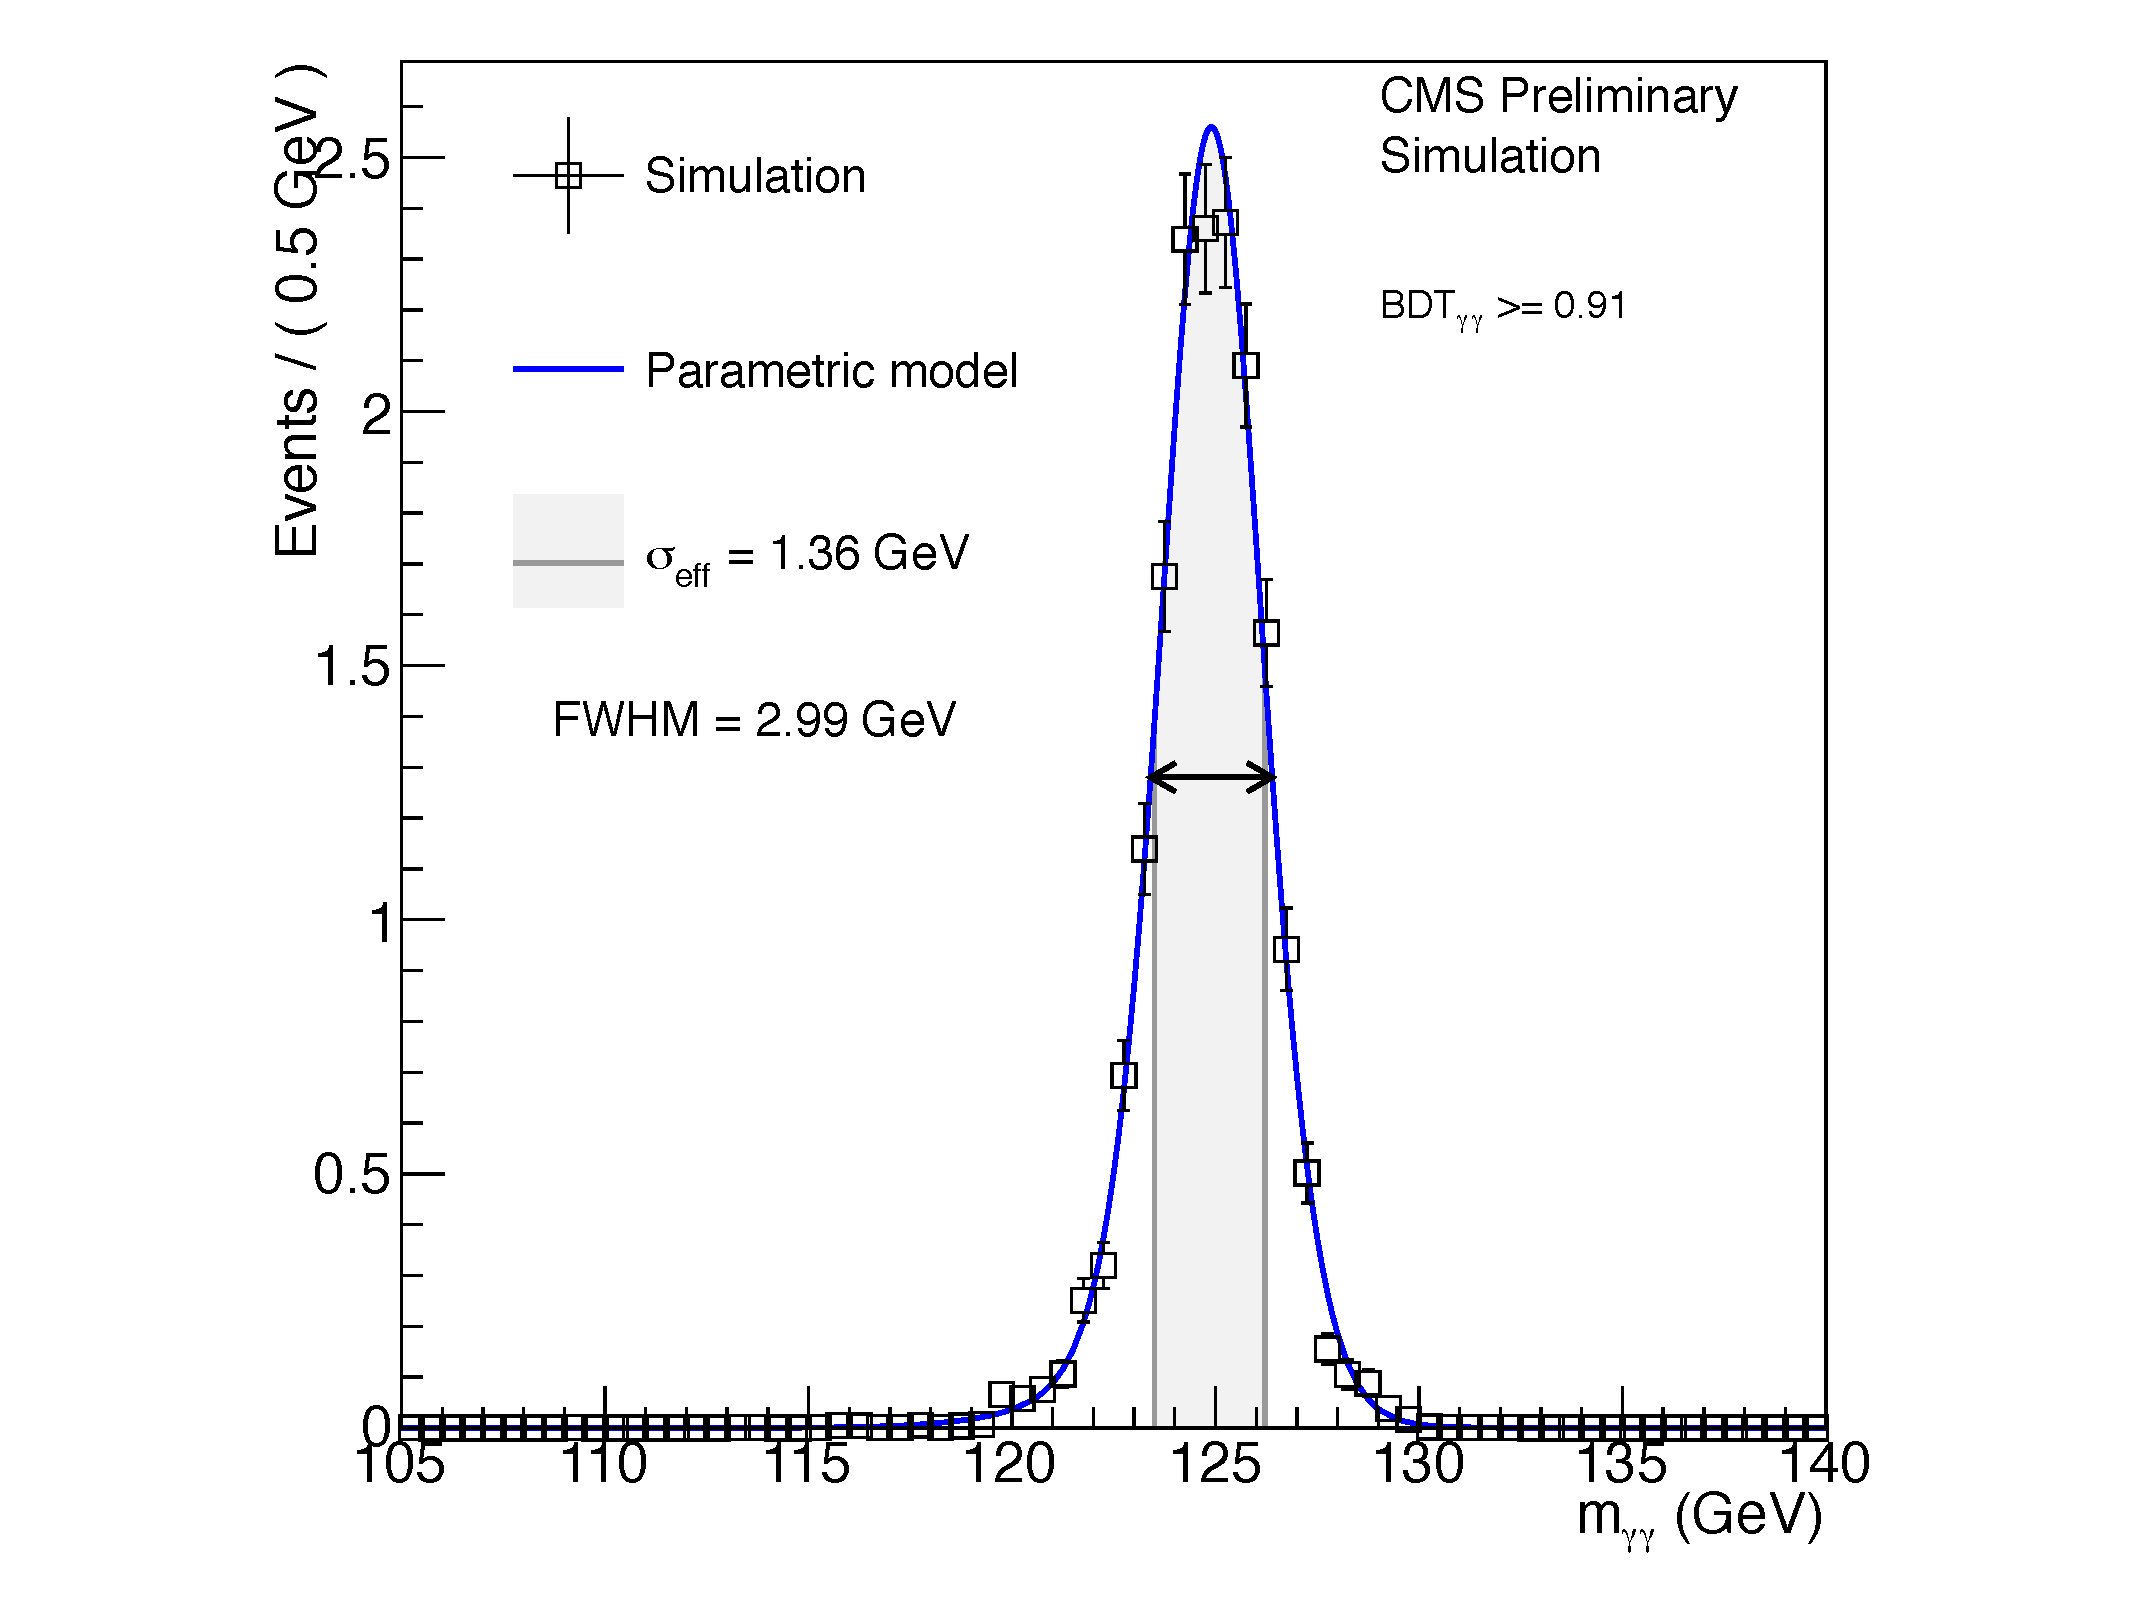
\includegraphics[width=0.38\textwidth]{CMS_DetectorFigures/ECAL_HiggsMassRes.pdf}
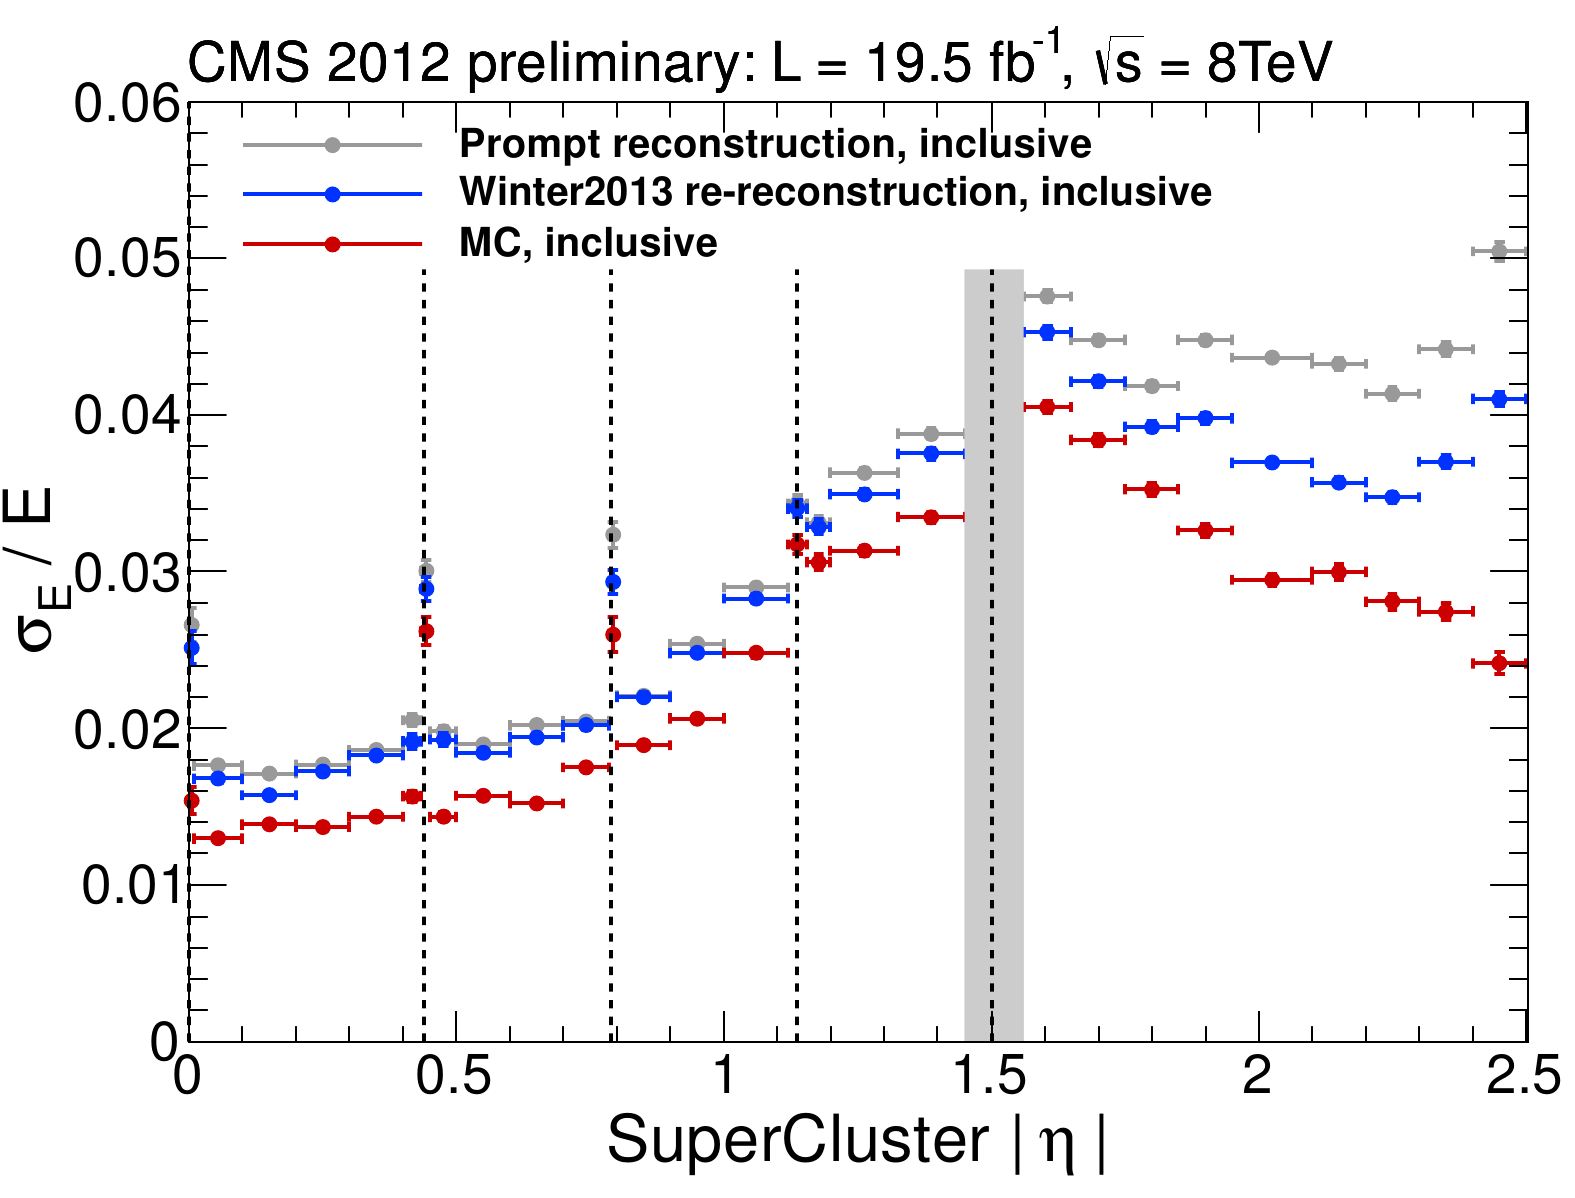
\includegraphics[width=0.49\textwidth]{CMS_DetectorFigures/EcalScaleEta_Incl.png}
\caption{The reconstructed Z invariant mass from $e^{+}e^{-}$
  decays. The left and right panels show the reconstructed invariant mass for
  the EB and EE, repectively, with different algorithms to reconstructed electron energies.\label{fig:ECAL_Higgs}}
\end{figure}
\section{The Hadronic Calorimeter}
The CMS Hadron Calorimeter (HCAL) is sorrounds the silicon tracker and
the electromagnetic calorimeter. It is composed of four different
subsytems: the barrel (HB), endcaps (HEs), the outer (HO), and the
forward (HF) calorimeters. The HB and HE are located inside the
cryostat of the superconducting solenoid and both are sampling
calorimeters with brass as the absorber and plastic scintillator as
the active meadium. The HO is plastic scintillator calorimeter located outside the superconducting
solenoid cryostat and is designed to catch the energy leakeage from
the HB. The HF is a quartz fiber and steel calorimeter located at $z
=\pm$ 11.15 m, thus, extending the pseudorapidity coverage up to
$|\eta| = 5$. The layout of the HCAL is presented in
Figure~\ref{fig:HCAL_Layout}.

\begin{figure}
 \centering
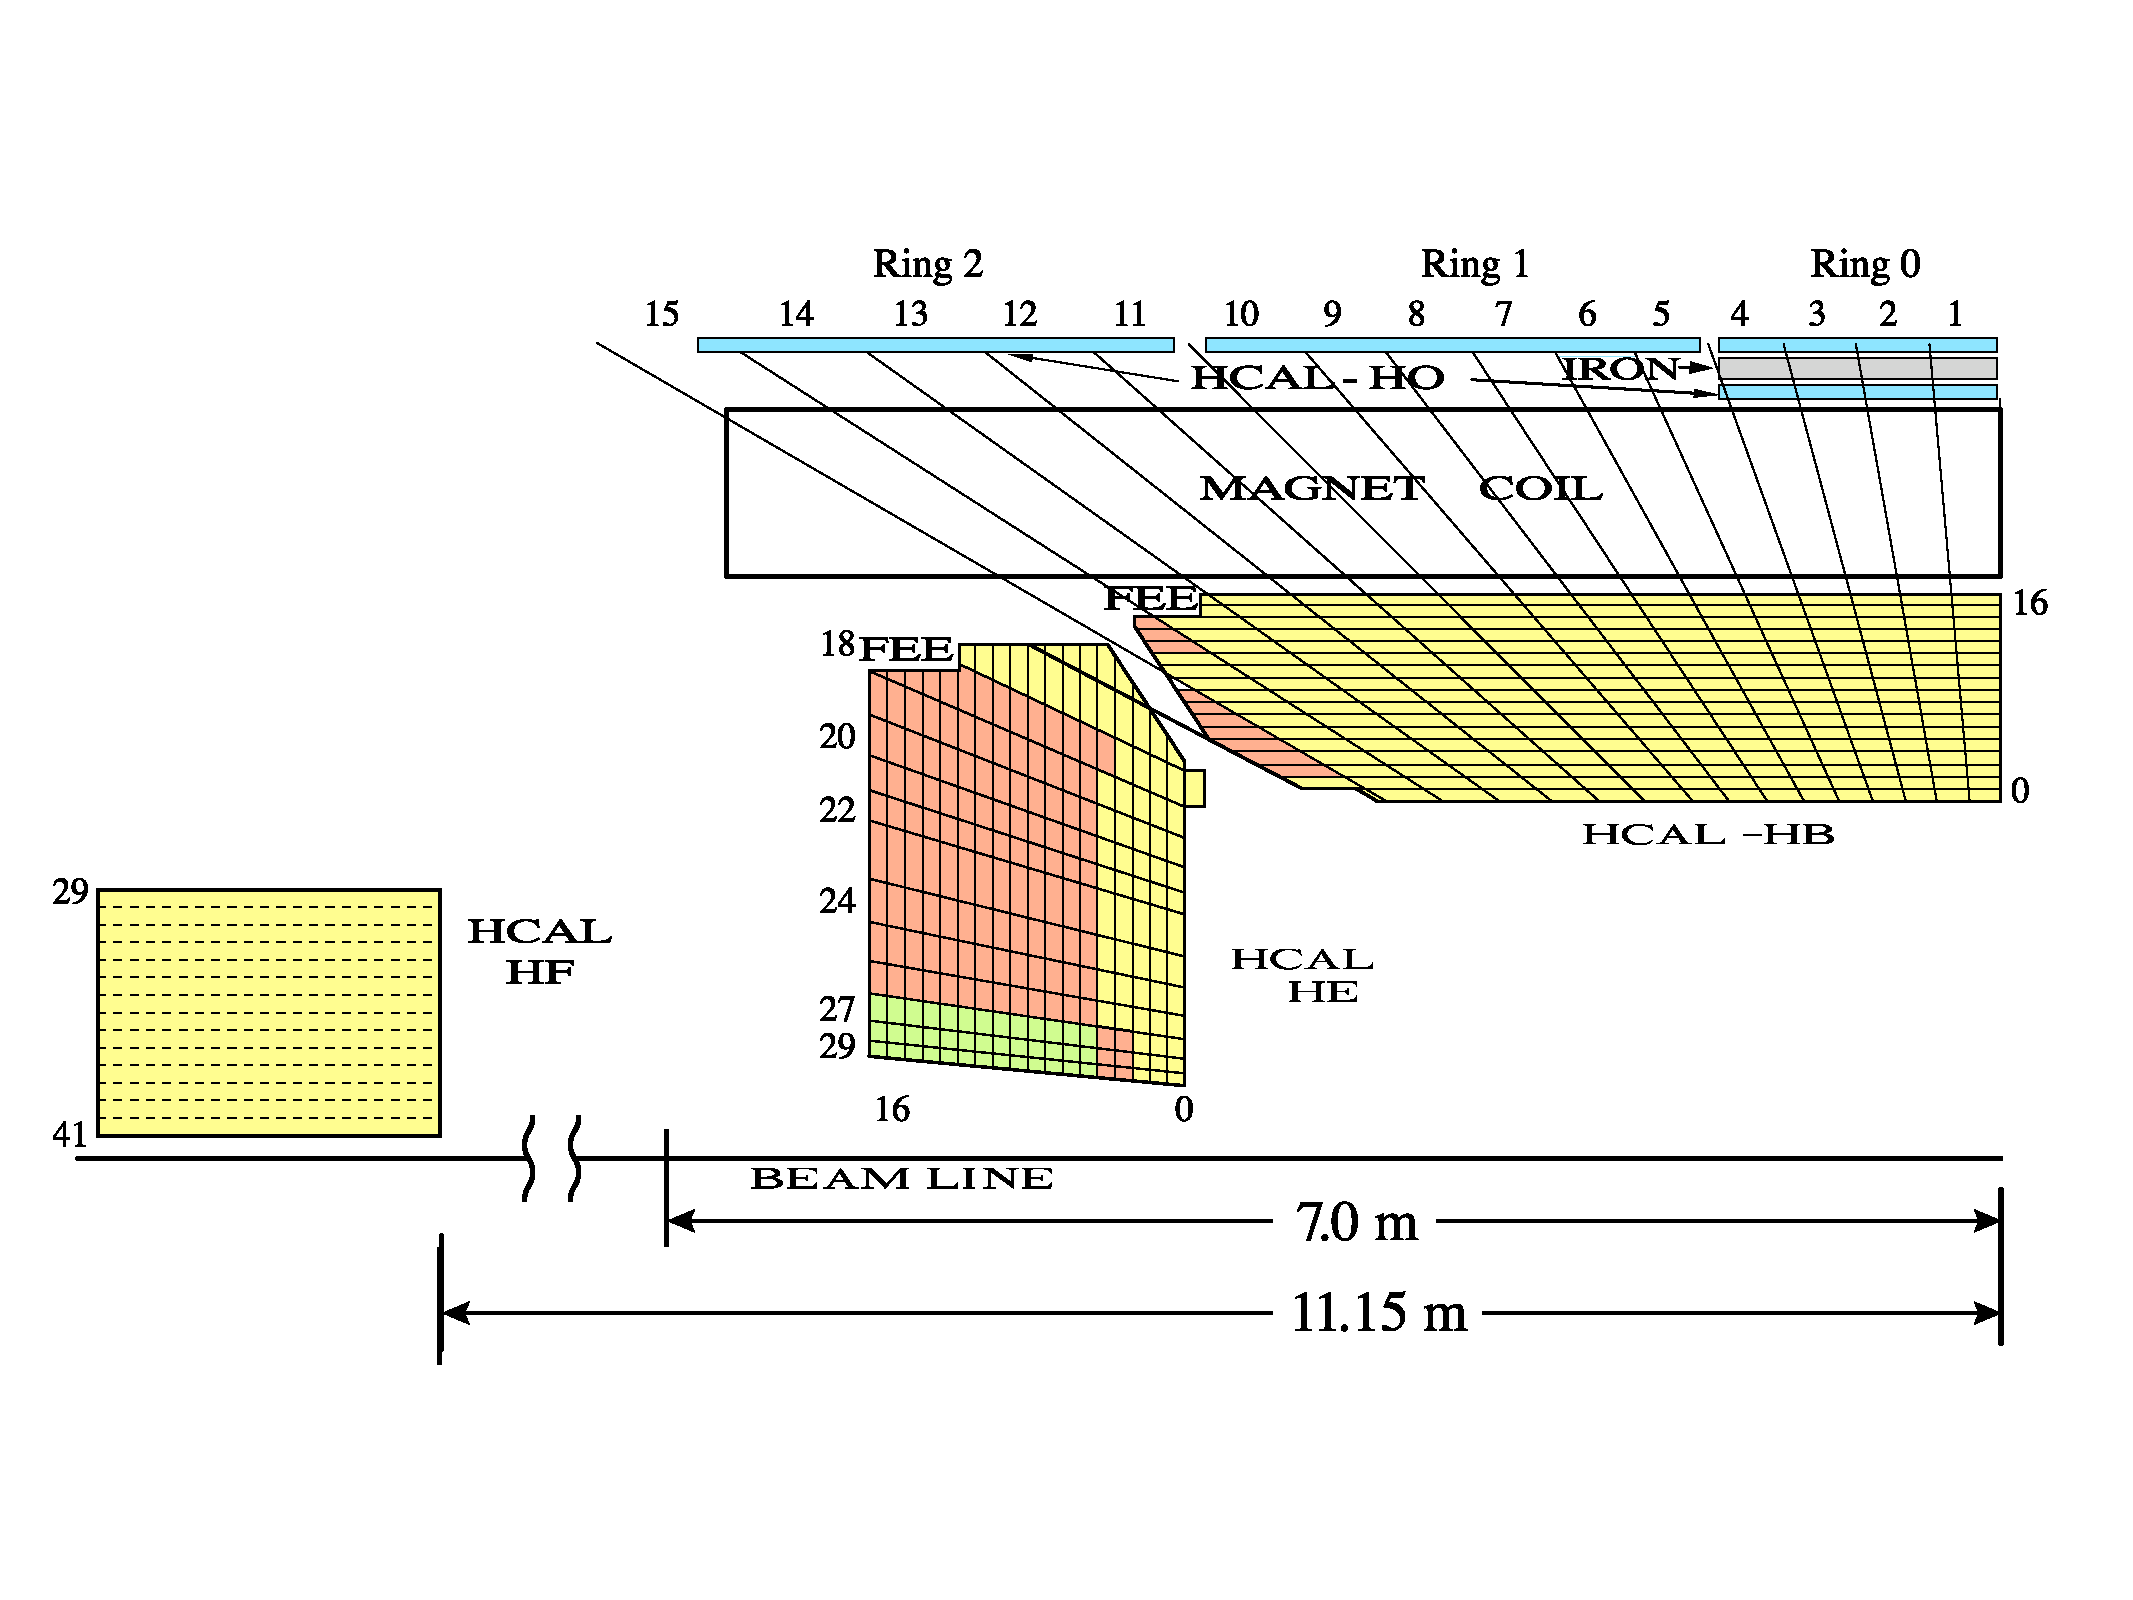
\includegraphics[width=0.99\textwidth]{CMS_DetectorFigures/HCAL_Layout.pdf}
\caption{The CMS HCAL layout.\label{fig:HCAL_Layout}}
\end{figure}

The hadronic energy resolution for the barrel HCAL and ECAL
combination was measured in beam test using pions and protons and
found to be:

\begin{equation}
\label{eq:hcal_res}
\frac{\sigma_{E}}{E} = \frac{0.847\pm0.016\GeV^{\frac{1}{2}}}{\sqrt{E
    (\GeV)}} \oplus 0.074\pm 0.008.
\end{equation}
The energy resolution in the endcaps is similar to that of the barrel.

The following passages are aimed to give a more detailed description
of the four HCAL subsystems.

\subsection{The Barrel Hadronic Calorimeter}
The HB is a sampling calorimeter made of brass absorber and plastic
scintillator as the active medium. The whole EB is build out of two
identical cylindrical structures, each of which is composed of 18
brass wedges. The pseudorapidity coverage of the HB reaches
approximately $|\eta| = 1.4$ while the $\phi$ covarage is
360$^{\circ}$. The segmentation of the HB is provided by the plastic
scintillator tiles inserted in the layers of the brass wedges, the later
are segmented into four $\phi$ sector, while there are 16 scintillator
tiles along the $\eta$ direction, thus providing the HB with an
equivalent segmentation of 0.087$\times$0.087 in $\eta$, $\phi$. Each
wedge calorimeter is composed of 16 layers of absorber and 17 layers of
plastic scintillator, the intermediate layer are made of brass
absorber and 3 mm plastic scintillator while the first and last layers
are made of stainless steel  and thicker 9 mm plastic scintillator
tiles. The very first layer is scintillator in order to detect showers
developed in the electromagnetic calorimeter
material. Figure~\ref{fig:HCALwedge} shows an schematic of a HB
wedge. The 16 scintillator tiles of each layer are laid in a tray in
order to facilitate their insertion and removal. Each tile's
scintillating light is collected by a green double-cladded
wavelength-shinting (WLS) fibers from Kuraray (Y-11) placed in groove
in the scintillator. Upon exiting the scintillating tile, each WLS is
splice into a clear fiber which subsequently ends in an optical
connector at the back of the tray. At this point, optical cables
take the light from the clear fiber into a 19 pixel hybrid photodiode
(HPD), which is designed to work inside the 3.8 T magnetic field. The
total interaction lengths ($\lambda_{I}$) of the HB varies with
pseudoparidity, there are 5.8 $\lambda_{I}$ at $\eta = 0$, increasing
up to 10.6 $\lambda_{I}$ at $|\eta| = 1.3$.
The finalized HB is shown in Figure~\ref{fig:hcal}.
\begin{figure}
 \centering
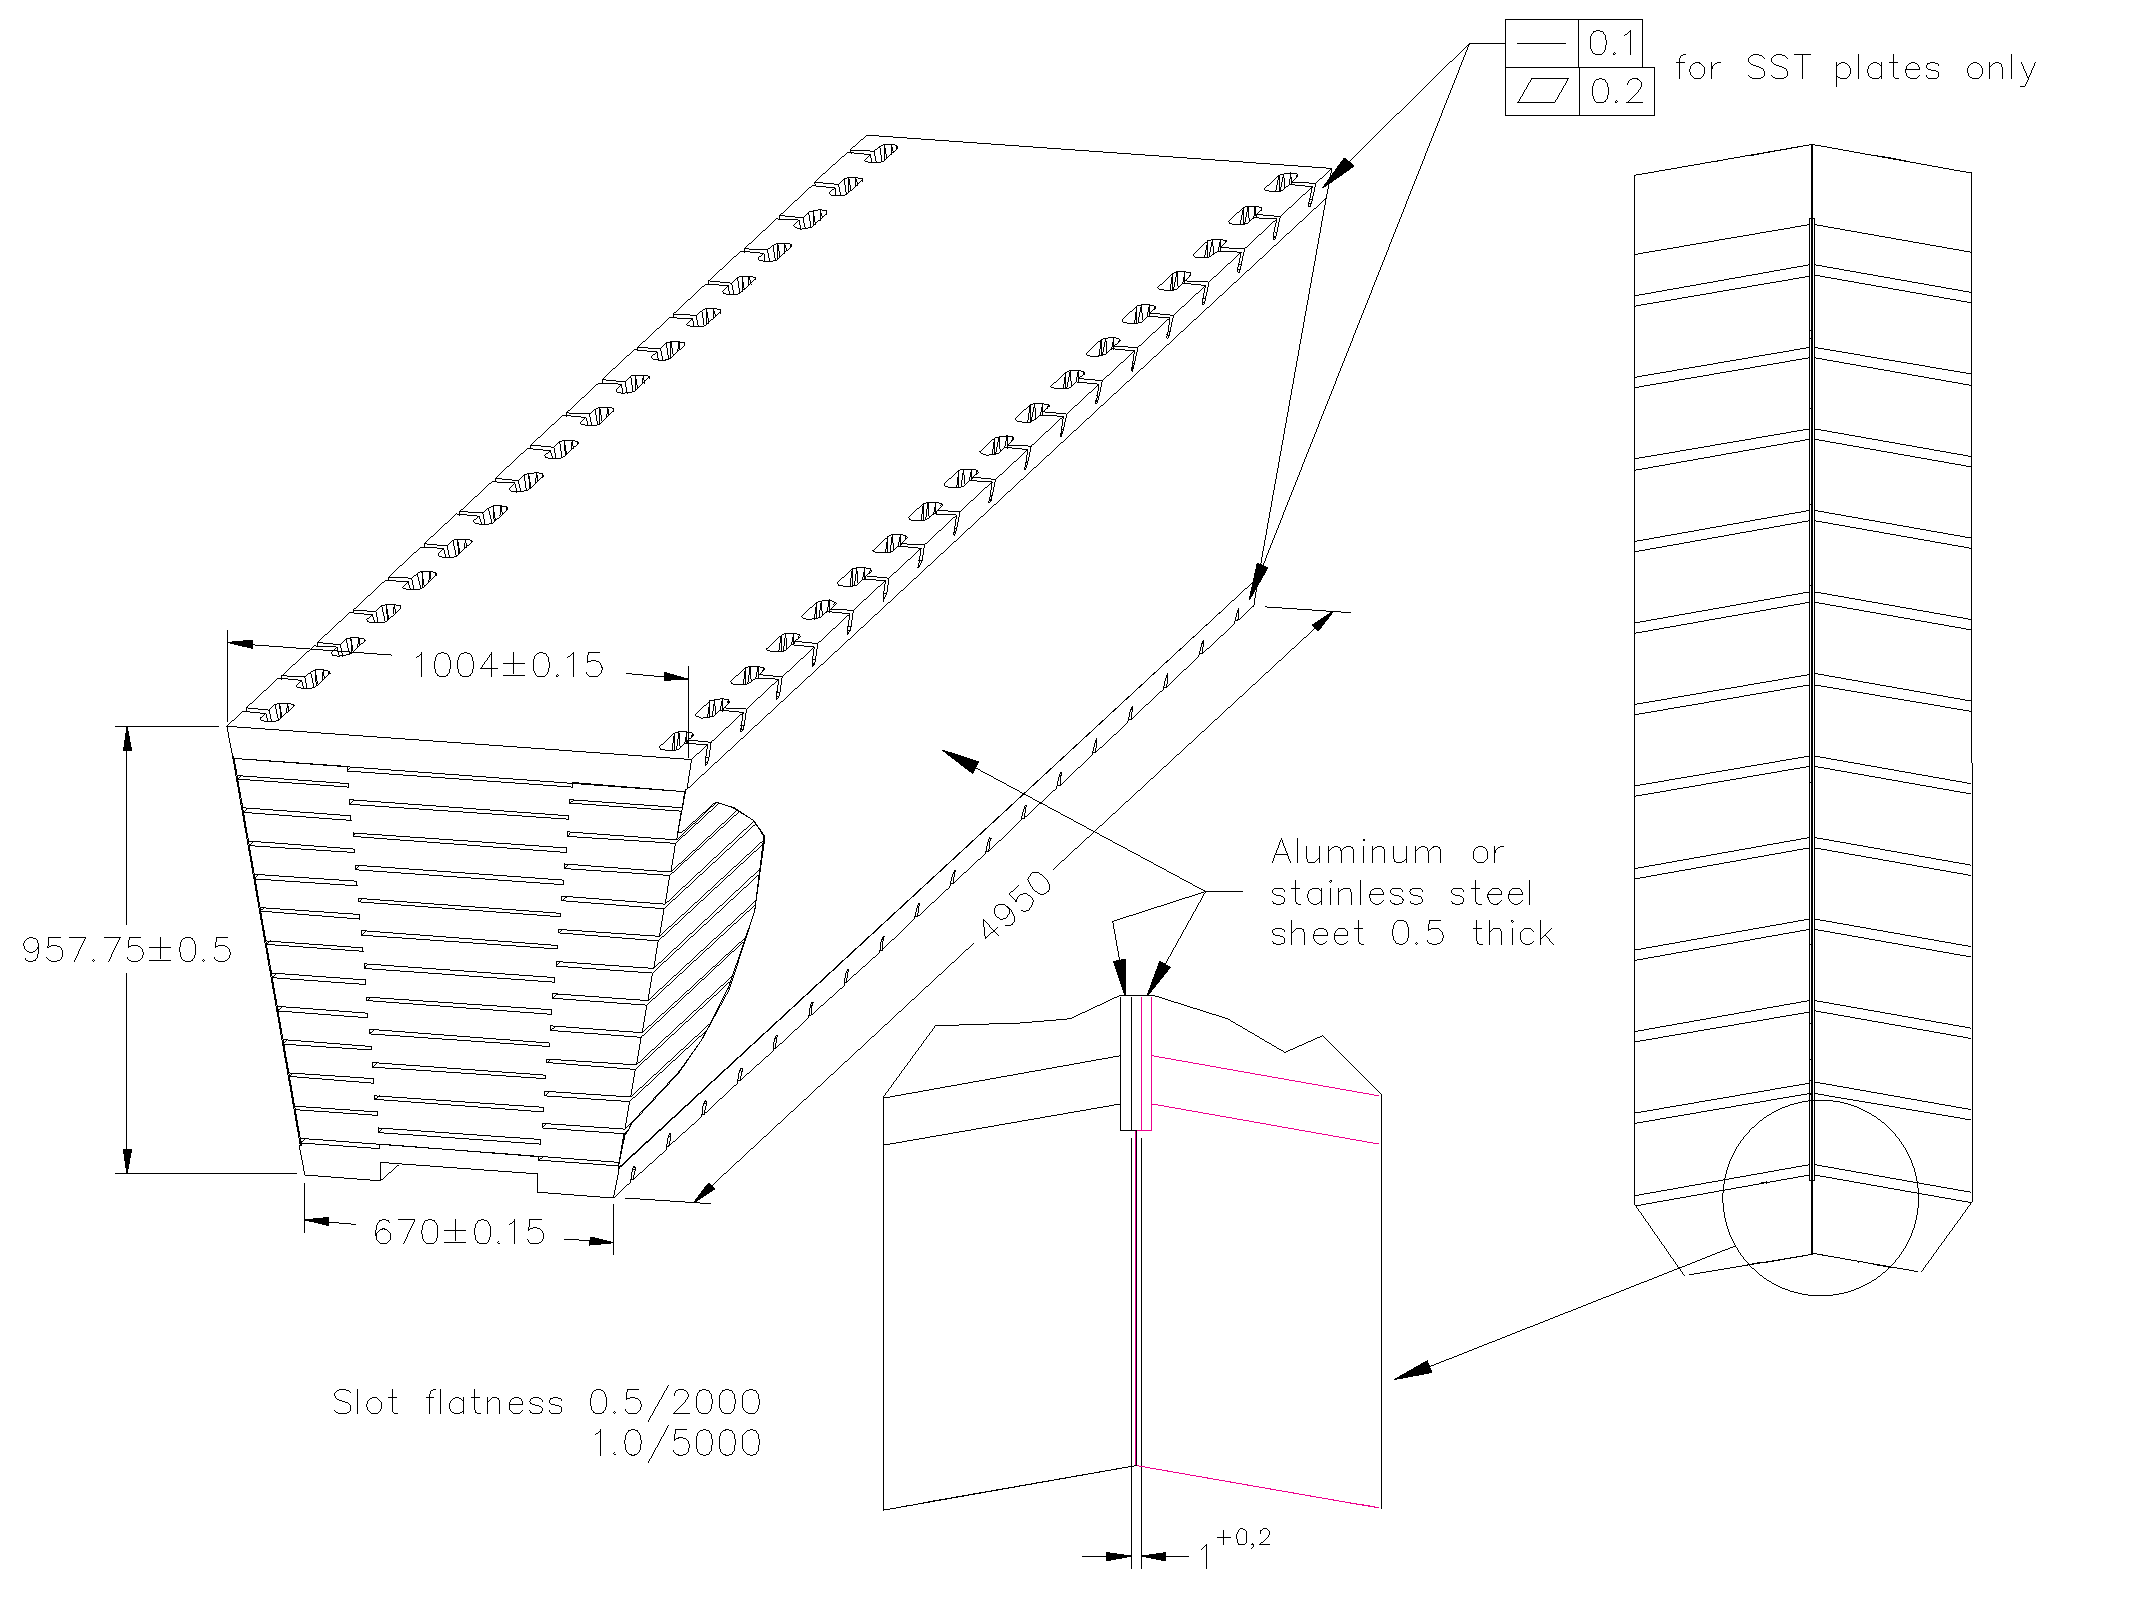
\includegraphics[width=0.99\textwidth]{CMS_DetectorFigures/HCAL_Wedge.pdf}
\caption{An schematic drawn of one of the wedges of the CMS HB.\label{fig:HCALwedge}}
\end{figure}
\begin{figure}
 \centering
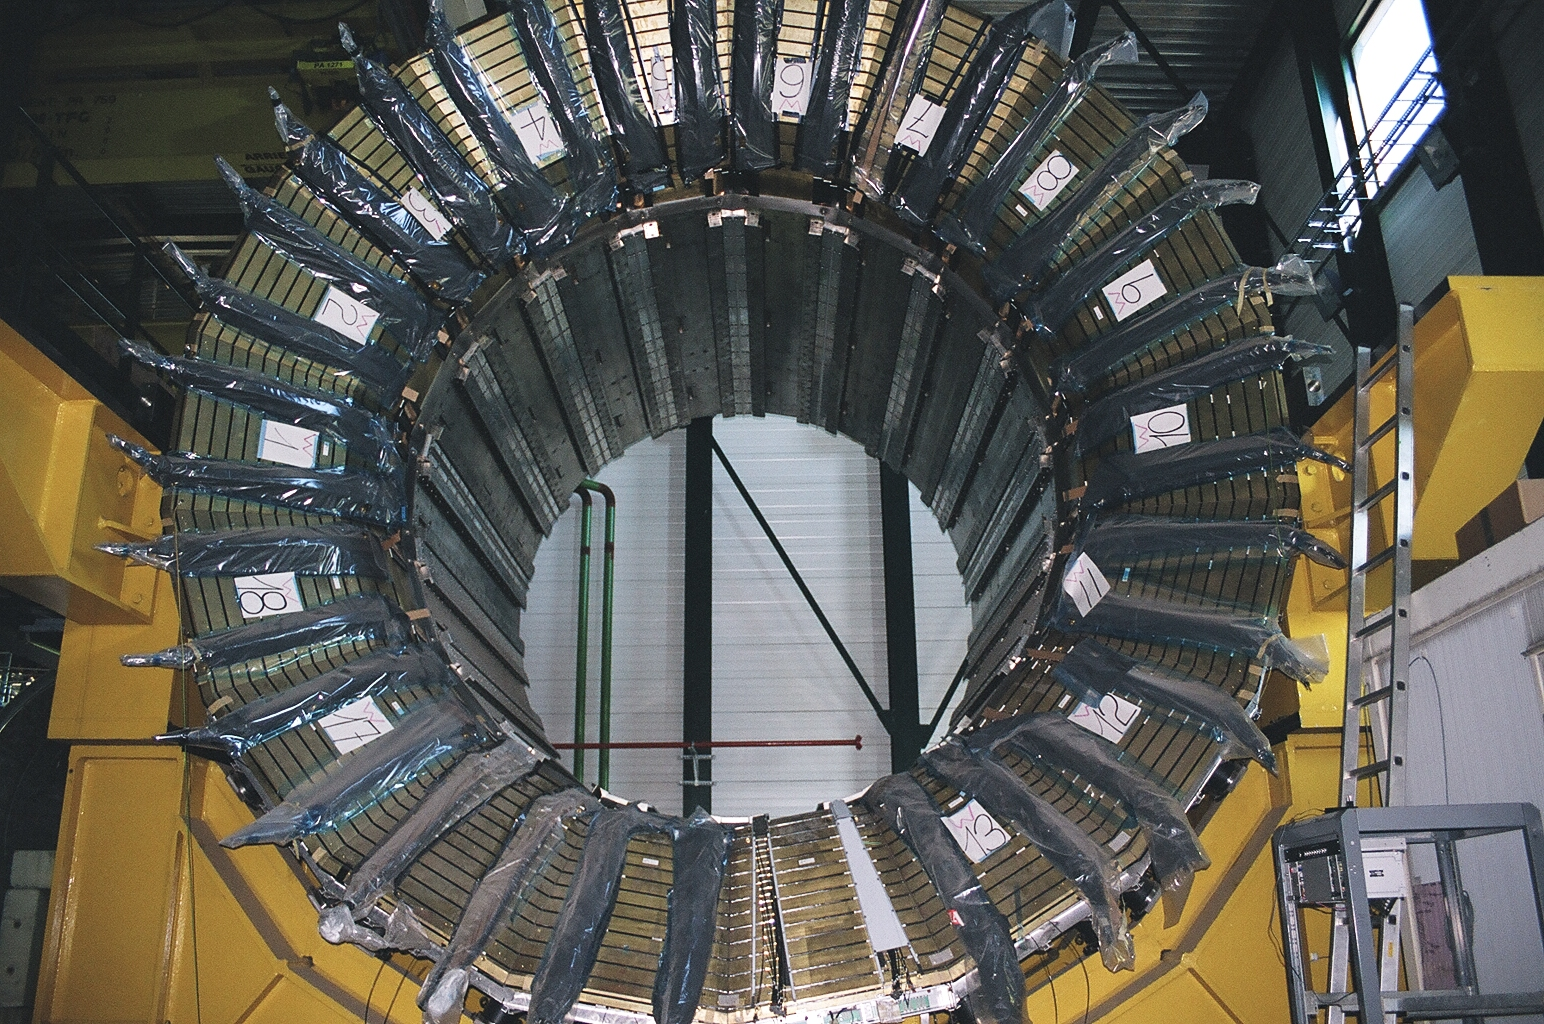
\includegraphics[width=0.99\textwidth]{CMS_DetectorFigures/hcal-HB.jpg}
\caption{A photograph of the finalized CMS HB.\label{fig:hcal}}
\end{figure}
\subsection{The Endcap Hadronic Calorimeter}
The HE is a brass/platic-scintillator sampling calorimeter that extend
the pseudorapidity coverage from $1.3 < |\eta| < 3$. It is composed of
79-mm-thick brass plates with 9 mm gaps to accomodate the
scintillator. The total material, including the crystals in the EE, is
about 10 $\lambda_{I}$. There are 18 layers -- along the $z$-direction
-- of plastic scintillators, the first layer, right after the EE, is
9-mm-thick, while the rest are 3-mm-thick. The scintillators are
segmented in the radial direction and their light is collected by
embedded WLS fiber. The scintillator tiles and the WLS are laid in
trays with a trapezoidal geometry. Figure~\ref{fig:HEtiles} shows an
schematic of the trays. The WLS are spliced to clear fibers which are
susequently terminated in an optical connector. Optical cables
transport the light from the optical connector the HPDs, which, as
mentioned earlier, could operate in the presense of a magnetic
field. This design results in a granularity of 0.087$\times$0.087
($\eta\times\phi$) for $|\eta| < 1.6$ and 0.17$\times$0.17 for $|\eta|
> 1.6$. Figure~\ref{fig:HE} shows one partially finalized HE, where
only some of the scintillator trays have been inserted.

\begin{figure}
 \centering
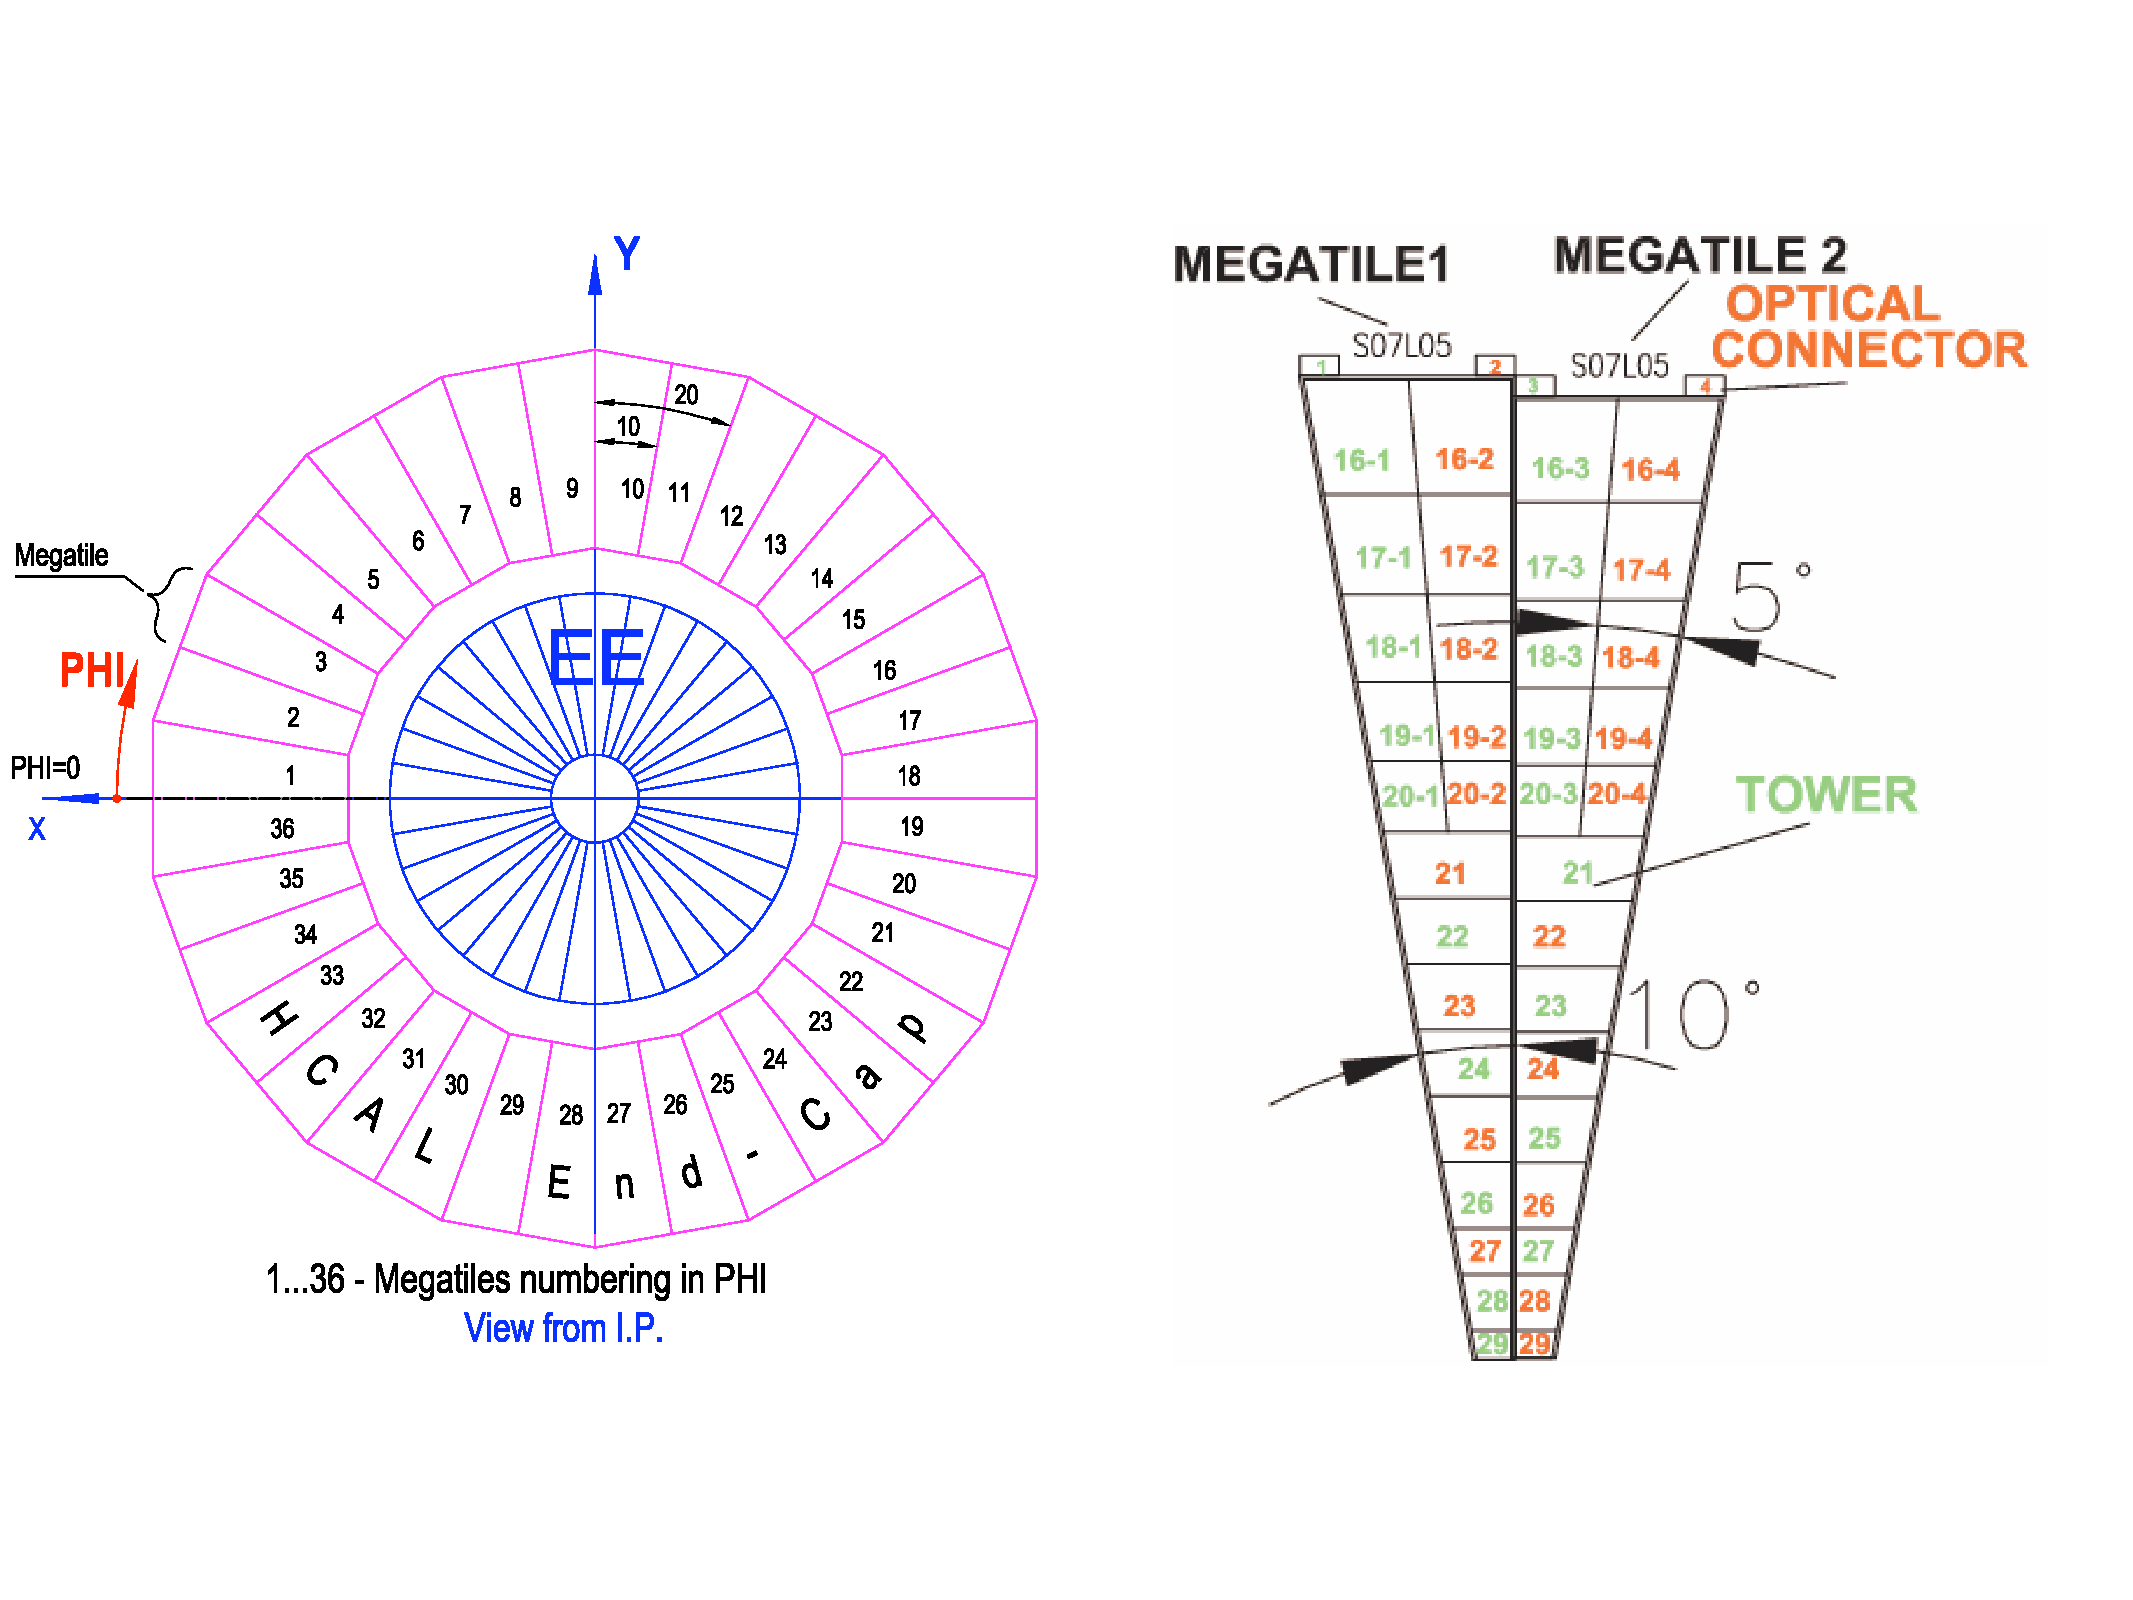
\includegraphics[width=0.99\textwidth]{CMS_DetectorFigures/hca_tile.pdf}
\caption{An schematic of the HE geometry in the $\phi$ direction is
  presented in the left panel. The configuration of two adjacent
  scintillator trays is presented in the right panel.\label{fig:HEtiles}}
\end{figure}
\begin{figure}
 \centering
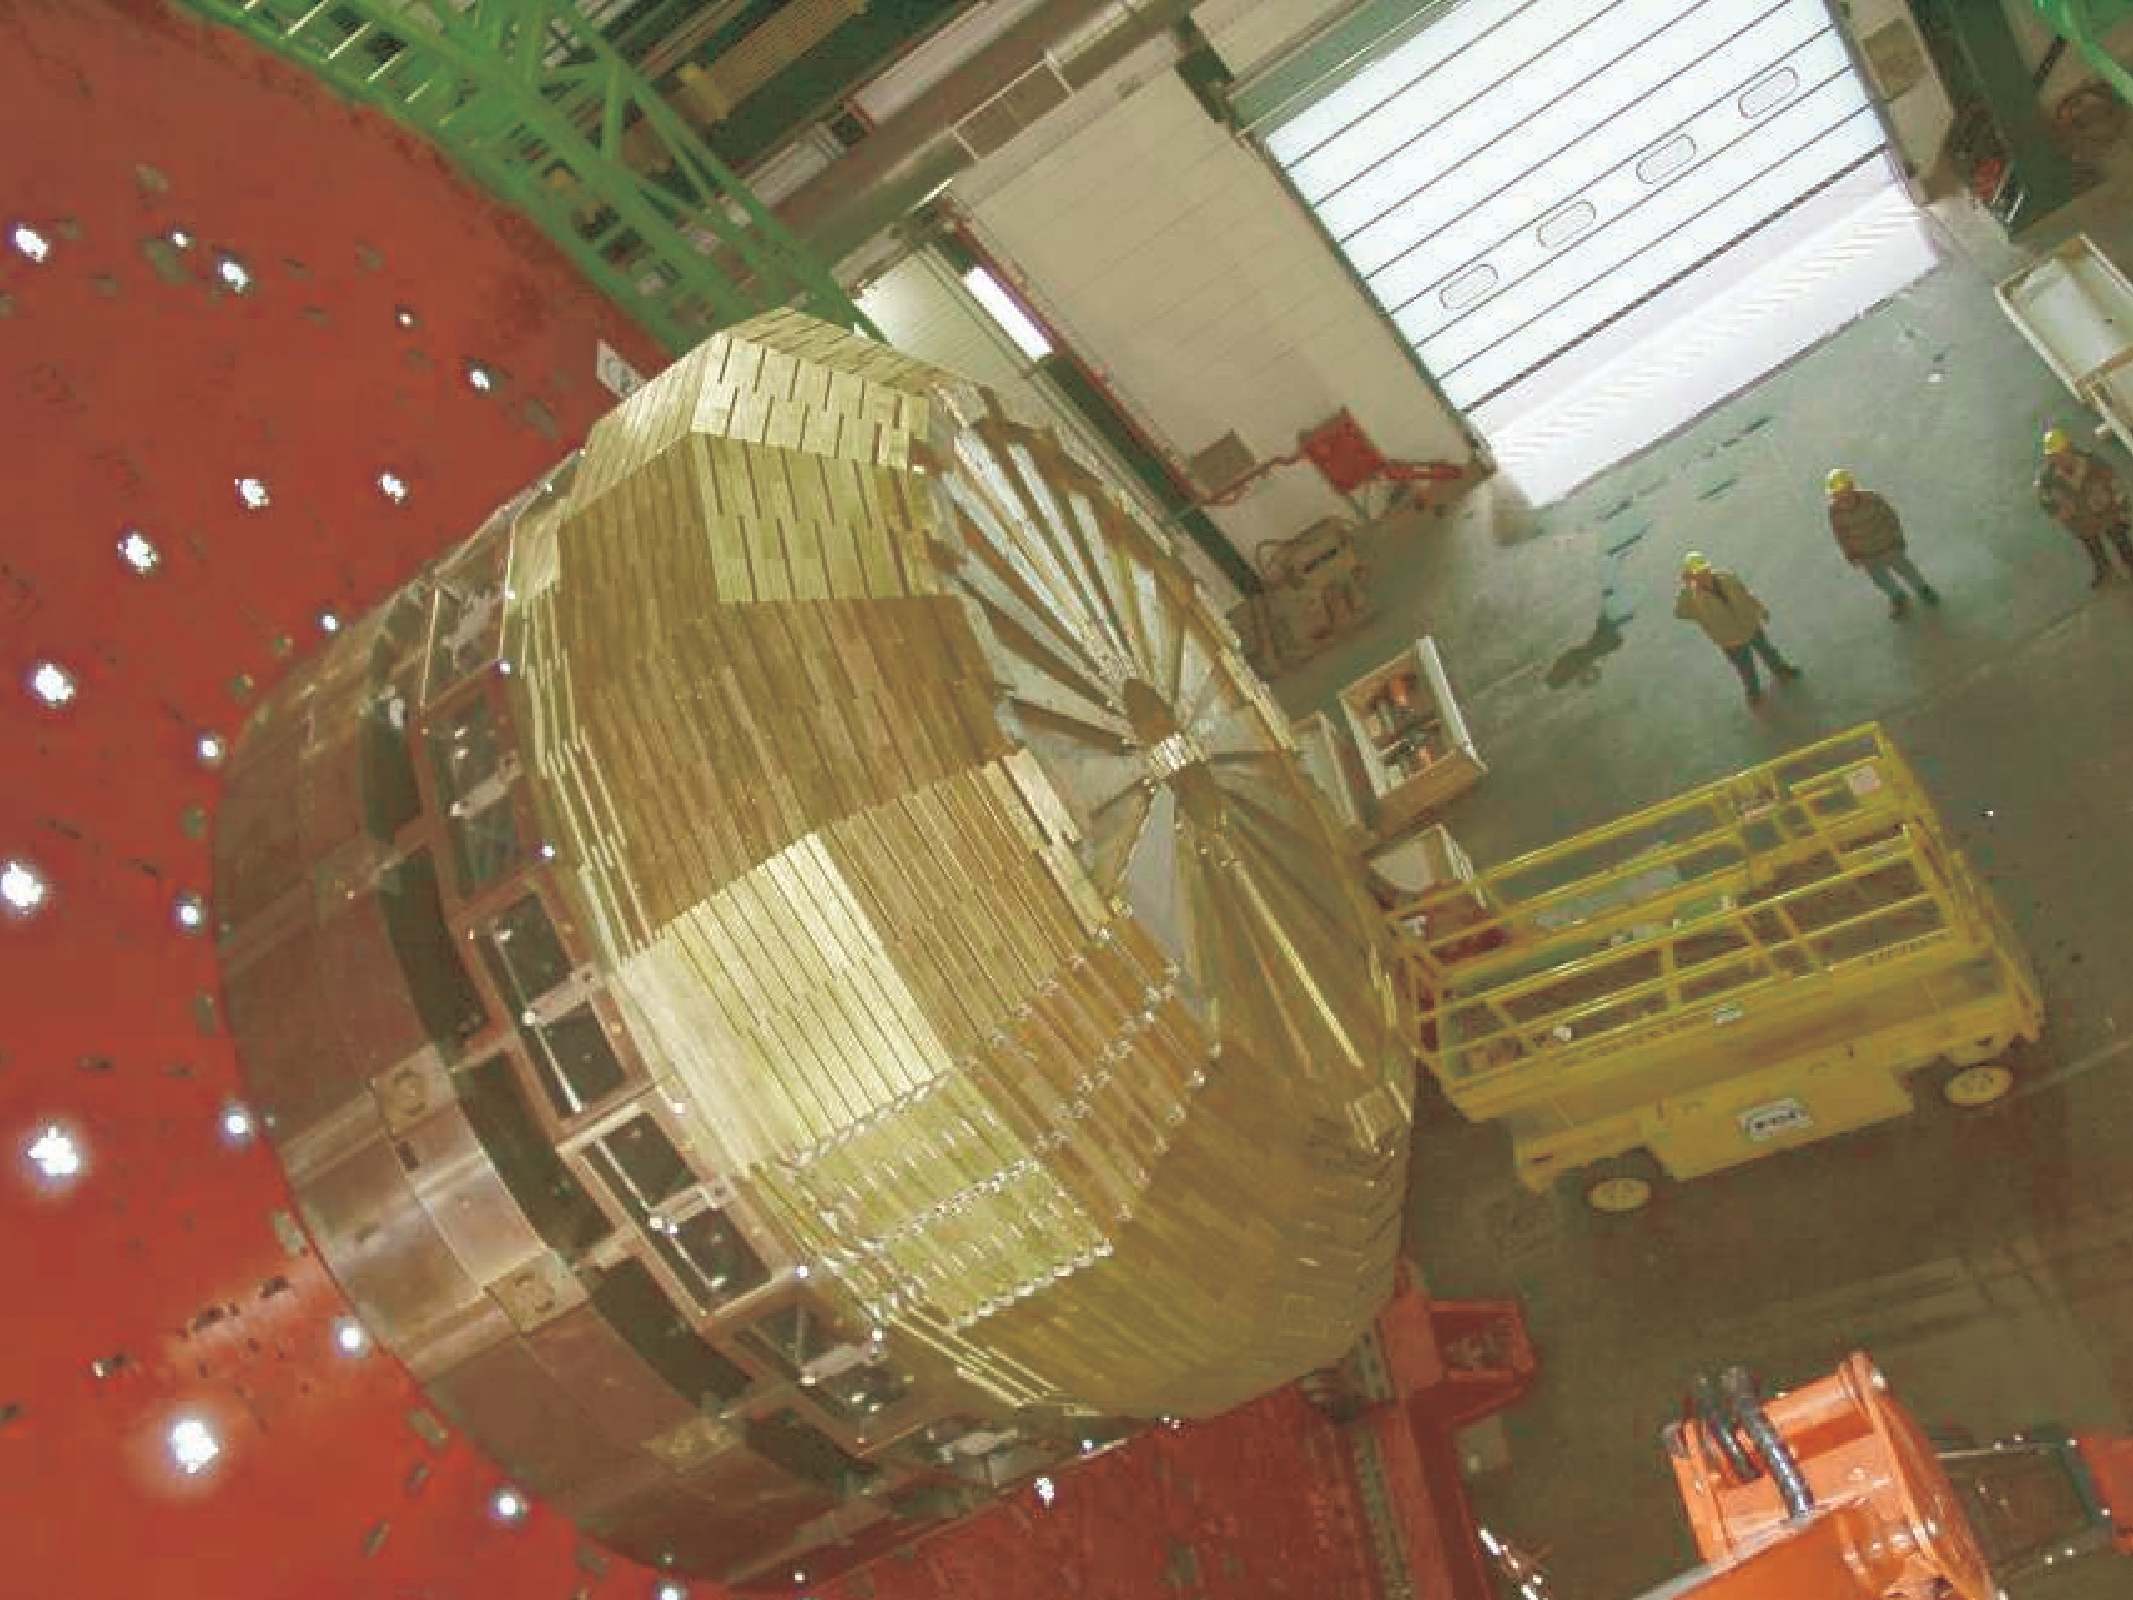
\includegraphics[width=0.99\textwidth]{CMS_DetectorFigures/hcal_HE.pdf}
\caption{A photograph of the one partially finalized CMS HE.\label{fig:HE}}
\end{figure}

\subsection{The Outer Hadronic Calorimeter}
\subsection{The Forward Hadronic Calorimeter}
\section{The Superconducting Solenoid}
\section{The Muon Chambers}
\section{Physics Object Reconstruction}
\section{Physics Object Reconstruction}
\subsection{Muon Identification}
\subsection{Electron and Photon Identification}
\subsection{Jet Identification}
\subsection{Missing Energy Reconstruction}
%%%%%%%%%%%%%%%%
%%%%% New Part%%%%
%%%%%%%%%%%%%%%%
\part{ Searches for New Physics with the Compact Muon Solenoid
  Experiment}

\chapter{Razor Approach to Search for BSM Physics}
\section{Introduction}
The challanges at hadron collider experiments are many, one of the
most well known is the fact the the energy and momentum of the parton-parton
(hard) interaction is not know. This limitation, in addition with the
fact that a large number of the proposed extensions of the SM (e.g. SUSY) predict
new particles that are weakly interacting and therefore escape the
detector systems without a trace, have made events with large momentum
imbalance in the plane transverse to the beam a key signature to
search for BSM physics. The momentum imbalance is the transverse plane
(missing energy)
is quantified by $\ptvecmiss$  which is defined as 
\begin{equation}
\label{eq:ptmiss}
\ptvecmiss = -\sum\limits_{i=0}^{n_{pf}} \vec{p}_{T}^{\hspace{0.06cm}i},
\end{equation}
where $\vec{p}_{T}^{\hspace{0.06cm}i}$ is the measured transeverse
momentum of a PF candidate, and $n_{pf}$ is the total number of PF
candidates reconstructed.

Additionally, in SUSY models with R-parity conservation the originally
pair produced super-partners undergo a cascade decay and at least two
particles (the LSPs) will escape detection and therefore further reduce the
hability to fully reconstruct the event kinematics due to the lost
information. Subsequently, all these effects result in lost of
sensitivity as the discrimination power between a possible
signal and the SM background processes is reduced. In order to recover
sensitivity, different kinematic variables are employed which are
functions of the visible objects momenta and the $\ptvecmiss$. These
kinematic variables have been shown to improve signal to background
discrimination but are often model dependent. One example of such
variables arew the razor variables~\cite{rogan,razor2010}, which have been widely used by the
CMS collaboration to search for
SUSY~\cite{Chatrchyan:2014goa,Razor8TeV} and recently shown to have
good sensitivity for DM direct production at hadron
colliders~\cite{Fox:2012ee}. The razor variables: $\MR$ and $\RR^2$  provide an estimate of the
underlying mass scale of the event and a handle to significantly
supress SM backgrounds -- particularly QCD multiijet --,
respectively. 

Since the two searches for BSM physics presented in this thesis are
based on the razor variables, this Chapter describes its derivation
(see Section~\ref{razorVariables})
and their main features when searching for new physics (see Section~\ref{razorApp}).

\section{The Razor Variables}\label{razorVariables}
The razor variables were originally derived~\cite{rogan,razor2010} for
squark pair-production in the context of SUSY; this topology is
represented by the Feynman diagram shown in Figure~\ref{fig:squarkpair}, where
the proton-proton collision pair produces two squarks ($\tilde{q}_{1}\tilde{q}_{2}$) which
subsequently decay into a SM quark and the LSP ($\tilde{q}_{i}\rightarrow q_{i}\tilde{\chi}_{1}^{0}$).

\begin{figure}
 \centering
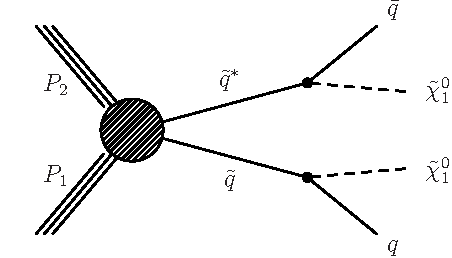
\includegraphics[width=0.4\textwidth]{RazorVariables/T2qq.pdf}
 \caption{Feynman diagram for squark pair-production.\label{fig:squarkpair}}
\end{figure}
One interesting quantity that provides access to the mass scale of the
SUSY particles is the magnitude of the 3-momentum of the quark in the
rest frame of the squark, it is actually more convenient to write down
twice this quantity:
\begin{equation}
\label{eq:pq}
2|\vec{p}^{\hspace{0.06cm}q_{i}}| =
2|\vec{p}^{\hspace{0.06cm}\tilde{\chi}_{1}^{0}}| =
\frac{\sqrt{m^{4}_{\tilde{q}} -
2m^{2}_{\tilde{q}}m^{2}_{\tilde{\chi}_{1}^{0}} +
m^{4}_{\tilde{\chi}_{1}^{0}} - 2m^{2}_{q}m^{2}_{\tilde{\chi}_{1}^{0}}
- 2m^{2}_{q}m^{2}_{\tilde{q}} + m_{q}^{4}}}{m_{\tilde{q}}},
\end{equation}
 where $m_{\tilde{q}}$ is the squark mass, $m_{\tilde{\chi}_{1}^{0}}$
 is the LSP mass, and $m_{q}$ is the SM quark mass. Eq.~\ref{eq:pq}
 can be simplified if the SM quarks are assumed massless -- which is
 mostly accurate with the exception of the top-quark. This
 simplification is also useful to define:
\begin{equation}
\label{eq:Mdelta}
M_{\Delta} = 2|\vec{p}^{\hspace{0.06cm}q_{i}}| =
\frac{m^{2}_{\tilde{q}} -
m^{2}_{\tilde{\chi}_{1}^{0}}}{m_{\tilde{q}}}.
\end{equation}

$M_{\Delta}$ is sensitive to the mass-splitting between the squark and
the LSP  and therefore is usually refer to as the characteristic mass
scale of the event. For example, in the case of the $W\rightarrow
\ell\nu$ decay, $M_{\Delta}$ is simply the mass of the W boson.

The razor variable \MR provides an estimate of $M_{\Delta}$ by
approximating the boosts needed -- since the actual boosts are
imposible to reconstruct due to the missing particles, which can be
viewed as an undetermined system of equations with not enough
contraints -- to go from the laboratory frame (lab frame) to the
squark rest frame. This approximation is done in two steps, first
, there is a common boost to go from the lab frame to the
center-of-momentum (CM) frame, and then, an equal and opossite boost
applied to each squark to go from the CM frame to their respective
rest frame. Figure~\ref{fig:restFrames} depicts the three frames and
the boosts needed to move from the lab frame to the squark rest frames.
\begin{figure}
 \centering
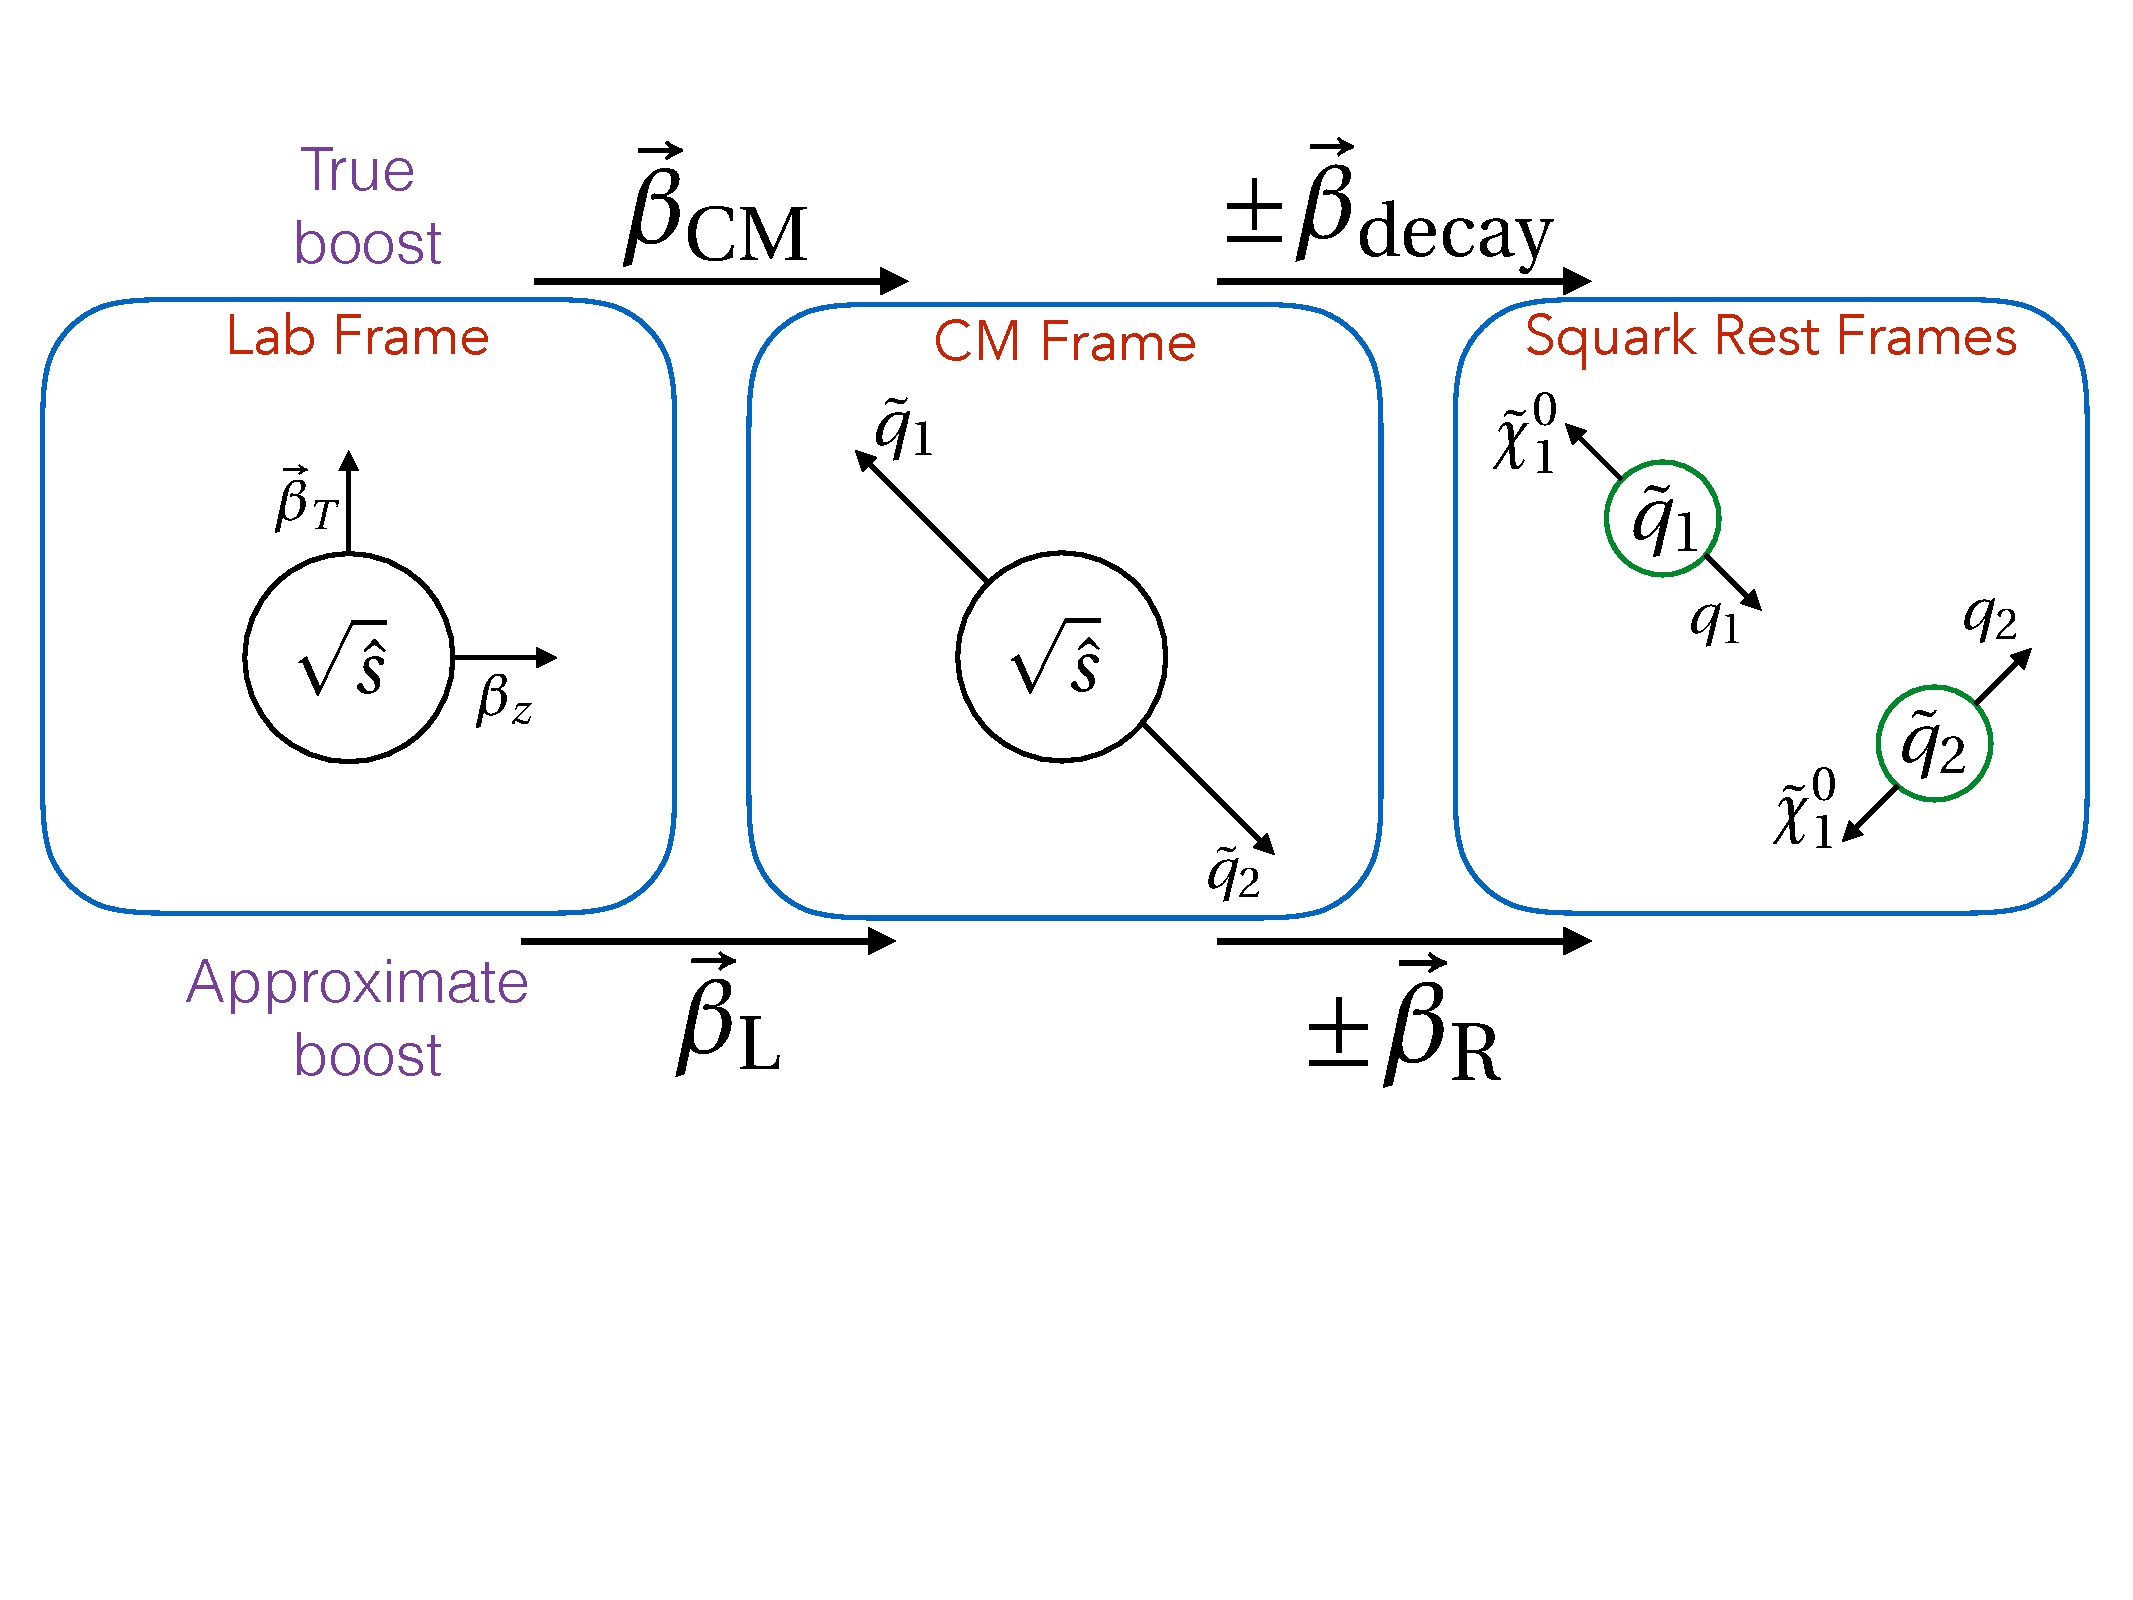
\includegraphics[width=1.0\textwidth]{RazorVariables/RazorFrameDiagram.pdf}
 \caption{An schematic of the  different rest frames involved in
   deriving the razor variables. The lab frame is in the left panel,
   the CM frame is in the middle panel, and the  squark rest frames
   are in the right panel.\label{fig:restFrames}}
\end{figure}  


\section{Application of the Razor Variables to Search for BSM Physics}\label{razorApp}


\chapter{Searches for Dark Matter at the LHC with 8 TeV pp collisions}\label{DMatLHC}
\section{Introduction}
The existence of dark matter (DM) in the universe, originally proposed~\cite{Zwicky:1937zza} to
reconcile observations of the Coma galaxy cluster with
the prediction from the virial theorem, is
commonly accepted as the explanation of many experimental
phenomena in astrophysics and cosmology, such as galaxy rotation
curves~\cite{vandeHulst,Rubin:1980zd}, large structure
formation~\cite{White:1987yr,Carlberg:1989yr,Springel:2005nw}, and the
observed
spectrum~\cite{Smoot:1992td,deBernardis:2000gy,Spergel:2006hy,Ade:2013zuv}
of the cosmic microwave background~\cite{Bardeen:1985tr}. A global fit to
cosmological data in the $\Lambda$CDM model (also known as
the standard model of cosmology)~\cite{Cen:2000xv} suggests that
approximately 85\% of the mass of the universe is attributable to
DM~\cite{Ade:2013zuv}. To accommodate these observations and the
dynamics of colliding galaxy clusters~\cite{Clowe:2006eq}, it has been
hypothesized that DM is made mostly of weakly
interacting massive particles
(WIMPs), sufficiently massive to be in nonrelativistic motion
following their decoupling from the hot particle plasma in the early
stages of the expansion of the universe.

While the standard model (SM) of particle physics does not include a
viable DM candidate, several models of physics beyond the SM, e.g.,
supersymmetry (SUSY)~\cite{Ramond,Golfand,Volkov,Wess,Fayet} with $R$-parity
conservation, can accommodate the existence of WIMPs. In these models,
pairs of DM particles can be produced in proton-proton (pp) collisions at
the CERN LHC. Dark matter particles would not leave a detectable signal in
a particle detector. When produced in association with high-energy
quarks or gluons, they could provide event topologies with
jets and a transverse momentum (\pt) imbalance ($\ptvecmiss$). The magnitude of $\ptvecmiss$ is referred to as missing transverse energy ($\ETm$).
The ATLAS and CMS collaborations have reported searches for events with one
high-\pt jet and large $\ETm$~\cite{Aad:2011xw,Chatrchyan:2012me}, which are sensitive to such topologies.
In this paper, we refer to these studies as monojet searches. Complementary studies of events with
high-\pt photons~\cite{Khachatryan:2014rwa,Aad:2014tda}; \PW,
\cPZ,~or
Higgs~bosons~\cite{Aad:2013oja,Aad:2014vka,Aad:2015dva,Aad:2015yga};
b jets~\cite{Aad:2014vea} and top quarks~\cite{Aad:2014vea,CMS:b2g12-022,CMS:semilepTop}; and leptons~\cite{ATLAS:2014wra,Khachatryan:2014tva}
have also been performed.

This paper describes a search for dark matter particles $\chi$ in events with at least two jets of comparable transverse momenta
and sizable $\ETm$. The search is based
on the razor variables $\MR$ and $\RR^2$~\cite{rogan,razor2010}.  Given a
dijet event, these variables are computed from the two jet momenta $\vv{p}^{j_1}$ and
$\vv{p}^{j_2}$, according to the following
definition:
 \begin{align}
 \begin{split}
 \MR  & =
 \sqrt{
  (\abs{\vv{p}^{j_1}}+\abs{\vv{p}^{j_{2}})^2 -
  (p^{j_1}_{z}+p^{j_2}_{z})^2}},
\\
 \mathrm{R}  & =   \frac{M^{\RR}_\mathrm{T}}{\MR},
\label{eq:razor}
\end{split}\\
\intertext{with}
 \label{eq:MTR}
 M^{\RR}_\mathrm{T}  &=   \sqrt{ \frac{\ETm(\pt^{j_1}+\pt^{j_2}) -
   \ptvecmiss {\cdot}
   (\vv{p}_{\mathrm{T}}^{\,j_1}+\vv{p}_{\mathrm{T}}^{j_2})}{2}}.
\end{align}

In the context of SUSY, $\MR$ provides an estimate of the
underlying mass scale of the event, and quantity $M^{\RR}_\mathrm{T}$ is a transverse
observable that includes information about the
topology of the event. The variable $\RR^2$ is designed to reduce QCD
multijet background; it is correlated with the angle
between the two jets, where co-linear jets have large $\RR^2$ while back-to-back jets have small $\RR^2$.
These variables have been used to study the production of non-interacting
particles in cascade decays of heavier partners, such as squarks and
gluinos in SUSY models with $R$-parity
conservation~\cite{Chatrchyan:2014goa,Razor8TeV}. The sensitivity of
these variables to direct DM production was suggested in
Ref.~\cite{Fox:2012ee}, where it was pointed out that the dijet event
topology provides good discrimination against background processes,
with a looser event selection than that applied in the monojet searches.
Sensitivity to DM production is most enhanced for large values of
$\RR^2$, while categorizing events based on the value of $\MR$
improves signal to background discrimination and yields significantly improved
search sensitivity to a broader and more inclusive class of DM models. 
The resulting sensitivity is expected to be 
comparable to that of monojet searches~\cite{Fox:2012ee,Papucci:2014iwa}. This
strategy also offers the possibility to search for DM particles that
couple preferentially to b quarks~\cite{Agrawal:2014una}, as proposed
to accommodate the observed excess of photons with energies between
1 and 4\GeV in the gamma ray spectrum of the galactic center data collected by the Fermi-LAT gamma-ray space
telescope~\cite{Hooper:2010mq}. The results are interpreted using an
effective field theory approach and the Feynman diagrams for DM pair production are shown in Fig.~\ref{fig:DMdiamgrams}.

\begin{figure}
 \centering
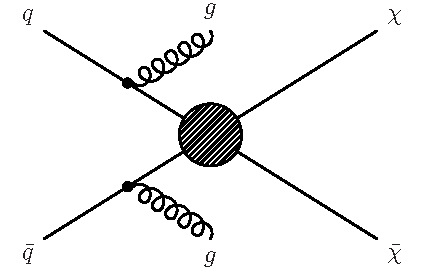
\includegraphics[width=0.35\textwidth]{Diagrams/RazorDMdiagram.pdf}
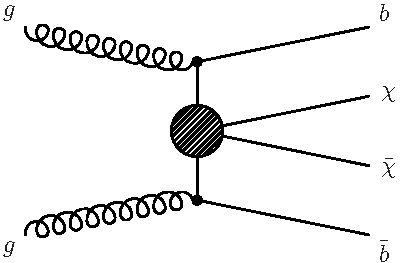
\includegraphics[width=0.35\textwidth]{Diagrams/dmdm_bbar.pdf}
 \caption{Feynman diagrams for the pair production of DM particles
   corresponding to an effective field theory using a vector or
   axial-vector operator (left), and a scalar operator (right).\label{fig:DMdiamgrams}}
\end{figure}


Unlike the SUSY razor searches~\cite{Razor8TeV,razor2010}, which focus on events with large
values of $\MR$, this study also considers events with small values
of $\MR$, using $\RR^2$ to discriminate
between signal and background, in a kinematic region ($\RR^2 >
0.5$) excluded by the baseline selection of Refs.~\cite{Razor8TeV,razor2010}.

A data sample corresponding to an integrated luminosity of
18.8\fbinv of pp collisions at a center-of-mass energy of 8\TeV  was collected by the CMS experiment
 with a trigger based on a
loose selection on $\MR$ and $\RR^2$. This and other
special triggers were operated in 2012 to record events at a rate
higher than the CMS computing system could process during data
taking. The events from these triggers were stored on tape and their
reconstruction was delayed until 2013, to profit from the larger availability of processing resources during the LHC shutdown.
These data, referred to as ``parked data''~\cite{CMS-DP-2012-022},
enabled the exploration of events with small $\MR$
values, thereby enhancing the sensitivity to direct DM production.

This paper is organized as follows:  section~\ref{sec:sample}
describes the data and simulated samples of events used in the
analysis. Sections~\ref{sec:selection} and~\ref{sec:sampleDef} discuss
the event selections and categorization, respectively. The
estimation of the background is described in Section~\ref{sec:bkg}.
The systematic uncertainties are discussed in Section~\ref{sec:sys},
while Section~\ref{sec:interpretation} presents the results and the
implications for several models of DM production. A summary is given in Section~\ref{sec:conclusions}.

% \section{The CMS detector}\label{cmsdetector}

% The central feature of the CMS apparatus is a superconducting solenoid
% of 6\unit{m} internal diameter, providing a magnetic field of
% 3.8\unit{T}. Within the solenoid volume are a silicon
% pixel and strip tracker, a lead tungstate crystal electromagnetic
% calorimeter (ECAL), and a brass and scintillator hadron calorimeter
% (HCAL), each composed of a barrel and two endcap sections.
% When combining information from the entire detector, the jet energy resolution amounts typically to 15\% at 10\GeV, 8\% at 100\GeV, and 4\% at 1\TeV~\cite{Chatrchyan:2013dga}. Muons are
% measured in gas-ionization detectors embedded in the steel flux-return
% yoke outside the solenoid. Forward calorimeters extend the
% pseudorapidity ($\eta$)~\cite{Chatrchyan:2008zzk} coverage provided by the
% barrel and endcap detectors. The first level (L1) of the CMS trigger system, composed of custom
% hardware processors, uses information from the calorimeters and muon
% detectors to select the most interesting events in a fixed time
% interval of less than 4\mus. The high-level trigger (HLT) processor
% farm further decreases the event rate from around 100\unit{kHz} to
% around 400\unit{Hz}, before data storage. A more
% detailed description of the CMS detector, together with a definition
% of the coordinate system used and the basic kinematic variables, can
% be found in Ref.~\cite{Chatrchyan:2008zzk}.

\section{Data set and simulated samples}
\label{sec:sample}
The analysis is performed on events with two jets reconstructed at L1
in the central part of the detector ($\abs{\eta}< 3.0$). The L1 jet
triggers are based on the sums of
transverse energy in regions $\Delta\eta\times\Delta\phi$
approximately 1.05$\times$1.05 in
size~\cite{Chatrchyan:2008zzk} (where $\phi$ is the azimuthal angle in the plane transverse to the LHC beams.).
At the HLT, energy deposits in ECAL and HCAL are clustered into jets and the
razor variables $\RR^2$ and $\MR$ are computed. In the
HLT, jets are defined using the {\FASTJET}~\cite{fastjet}
implementation of the anti-\kt~\cite{antikt} algorithm, with
a distance parameter equal to 0.5. Events with at least two jets
with $\pt>64$\GeV are
considered. Events are selected with $\RR^2> 0.09$ and
$\RR^2 \times \MR > 45$\GeV. This selection
rejects the majority of the background, which tends to have low $\RR^2$ and low
$\MR$ values, while keeping the events in the signal-sensitive
regions of the ($\MR$, $\RR^2$) plane.
The trigger efficiency, measured using a pre-scaled trigger with very loose thresholds, is
shown in Table~\ref{tab:Trigger}.  The requirements described above correspond to the least stringent event selection, given the constraints on the maximum acceptable rate.

\begin{table}[htb]
\centering
  \topcaption{\label{tab:Trigger}Measured trigger efficiency for different
    $\MR$ regions. The selection $\RR^2 > 0.35$ is applied. The uncertainty
    shown represents the statistical uncertainty in the measured efficiency.
}
\begin{tabular}{cccc}
  \hline
  $\MR$ region (\GeVns{}) & 200--300 &  300--400 &
  400--3500 \rule{0pt}{2.3ex} \rule[-1.2ex]{0pt}{0pt}\\
  \hline
  Trigger efficiency (\%) & $91.1\pm ^{1.5}_{1.7}$ &
  $90.7\pm^{2.3}_{2.9}$ & $94.4 \pm ^{2.4}_{3.6}$ \rule{0pt}{2.3ex} \rule[-1.2ex]{0pt}{0pt}\\
  \hline
\end{tabular}
\end{table}

Monte Carlo (MC) simulated signal and background samples are generated with the
leading order matrix element generator {\MADGRAPH
  v5.1.3}~\cite{Alwall:2011uj,Alwall:2014hca} and the CTEQ6L parton
distribution function set~\cite{Pumplin:2002vw}. The generation
includes the \PYTHIA 6.4.26~\cite{Sjostrand:2006za} Z2* tune, which is
derived from Z1 tune~\cite{Field:2010bc} based on the CTEQ5L set.
Parton shower and hadronization effects are included by matching the generated events to \PYTHIA, using the MLM matching algorithm~\cite{Hoche:2006ph}.
The events are processed with a \GEANTfour~\cite{G4} description of the CMS apparatus to include
detector effects. The simulation samples for SM
background processes are scaled to the
integrated luminosity of the data sample (18.8\fbinv), using
calculations of the inclusive production cross sections at the next-to-next-to-leading
order (NNLO) in the perturbative QCD
expansion~\cite{WatNNLO,ZatNNLO,TTbaratNNLO}.
 The signal processes corresponding to pair production of DM particles
 are simulated with up to two additional partons with $\pt>80$\GeV.

\section{Event selection}\label{sec:selection}

Events are selected with at least one reconstructed
interaction vertex within $\abs{z}<24$\cm. If more than one vertex is
found, the one with the highest sum of the associated track momenta squared is used as the
interaction point for event reconstruction. Events containing
calorimeter noise, or large missing transverse momentum
due to beam halo and instrumental effects (such as jets near
non-functioning channels in the ECAL) are removed from the analysis~\cite{MET_8TeV}.

A particle-flow (PF) algorithm~\cite{PF1,CMS-PAS-PFT-10-001} is used to reconstruct
and identify individual particles with an optimized combination of
information from the various elements of the CMS detector. The energy
of photons is directly obtained from the ECAL measurement, corrected
for zero-suppression effects. The energy of electrons is determined
from a combination of the electron momentum at the primary interaction
vertex as measured by the tracker, the energy of the corresponding
ECAL cluster, and the energy sum of all bremsstrahlung photons (or emissions)
spatially compatible with originating from the electron track. The
energy of muons is obtained from the curvature of the associated
track. The energy of charged hadrons is determined from a combination
of their momentum measured in the tracker and the matching ECAL and
HCAL energy deposits, corrected for zero-suppression effects and for
the response function of the calorimeters to hadronic
showers. Finally, the energy of neutral hadrons is obtained from the
corresponding corrected ECAL and HCAL energies. Contamination of the
energy determinations from other pp collisions is mitigated by
discarding the charged PF candidates incompatible with originating from the main vertex.  Additional
energy from neutral particles is subtracted on average when computing
lepton (electron or muon) isolation and jet energy. This contribution is estimated as the
per-event energy deposit per unit area, in the cone $\Delta R = \sqrt{\smash[b]{(\Delta
  \eta)^2+(\Delta\phi)^2}}=0.3$, times the considered jet size or
isolation cone area.

Electrons (muons) are required to have $\pt>15$\GeV and  $\abs{\eta}<2.5$
(2.4). In order to reduce the
background from hadrons misidentified as leptons, additional
requirements based on the
quality of track reconstruction and isolation are applied. Lepton isolation is
defined as the scalar \pt sum of all PF candidates other than the
lepton itself, within a cone of size $\Delta R = 0.3$, and normalized to the lepton \pt. A
candidate is identified as a lepton if the isolation variable is found to be smaller than 15\%.
For electrons~\cite{ElectronsCMS}, a characteristic of the shower
shape of the energy deposit in the ECAL (the shower width in the
$\eta$ direction) is used to further reduce the contamination from hadrons.
PF candidates with $\pt > 10$\GeV that are not consistent with muons and satisfy the same isolation
requirements as those used for electrons are also identified to increase the 
lepton selection efficiency as well as to identify single-prong tau decays. 


Jets are formed by clustering the PF candidates, using the anti-\kt algorithm with distance
parameter 0.5. Jet momentum is determined as the vectorial sum of all
particle momenta in the jet, and is found from simulation to be within
5\% to 10\% of the generated hadron level jet momentum over the whole \pt spectrum and
detector acceptance.
 Jet energy corrections
are derived from simulation, and are confirmed with in situ
measurements of the energy balance in dijet and photon+jet events.
Additional selection criteria are applied to each event to remove
spurious jet-like features originating from isolated noise patterns in certain HCAL regions.
We select events containing at least two jets with $\pt>80$\GeV and $\abs{\eta}<2.4$, for
which the corresponding L1 and HLT requirements are maximally
efficient. The combined secondary vertex (CSV) b-tagging
algorithm~\cite{btag8TeV,btag7TeV} is used to identify jets originating from b
quarks. The loose and tight working points of the CSV algorithm, with
85\% (10\%) and 50\% (0.1\%) identification efficiency (misidentification probability) respectively, are
used to assign the selected events to categories based on the number
of b-tagged jets, as described below.

In order to compute the razor variables inclusively, the event is forced into a two-jet topology, by forming two \textit{megajets}~\cite{Chatrchyan:2014goa} out of all the reconstructed
jets with $\pt>40$\GeV and $\abs{\eta}<2.4$. All possible assignments of
jets to the megajets are considered, with the requirement that a
megajet consist of at least one jet. The sum of the four-momenta of
the jets assigned to a megajet defines the megajet
four-momentum. When more than two jets are reconstructed, more than
one megajet assignment is possible. We select the assignment that
minimizes the sum of the invariant masses of the two megajets.
In order to reduce the contamination from multijet production, events are
rejected if the angle between the two selected megajets in the
transverse plane $\abs{ \Delta\phi (j_{1}, j_{2})}$ is larger
than 2.5 radians. The momenta of the two megajets are used to compute
the razor variables, according to Eq.~(\ref{eq:razor},~\ref{eq:MTR}).  Events are
required to have $\MR>200$\GeV and $\RR^2>0.5$.

\section{Analysis Strategy}\label{sec:sampleDef}

To enhance the DM signal and suppress background contributions from the $\PW$+jets and $\ttbar$ processes,
we veto events with selected electrons, muons, or isolated charged PF candidates.
We define three different search regions based on the number of b-tagged jets. 
The zero b-tag search region contains events where no jets were identified with the CSV loose 
b-tagging criterion; the one b-tag search region contains events where exactly one jet
passed the CSV tight criterion; and the two b-tag search region contains events where two or more
jets passed the CSV tight criterion. Events in the zero b-tag search region are further classified 
into four categories based on the value of $\MR$, to enhance signal to background
discrimination for a broad class of DM models: 
(i) \textit{very low} $\MR$ (VL), defined by $200<\MR \leq 300$\GeV; 
(ii) \textit{low} $\MR$ (L), with $300 <\MR \leq 400$\GeV; 
(iii) \textit{high} $\MR$ (H), with $400 <\MR\leq 600$\GeV; 
and (iv) \textit{very high} $\MR$ (VH), including events with $\MR>600$\GeV. 
Because of the limited size of the data sample, no further 
categorization based on $\MR$ is made for the one and two b-tag search regions.
Within each category, the search is performed in bins of the $\RR^2$
variable, with the binning chosen such that the expected background yield
in each bin is larger than one event, as estimated from Monte Carlo simulation.
In the H and VH categories, 3\% and 35\% respectively of the selected
events were also selected in the monojet search~\cite{monojet8TeV}, which used data from the same running period. The overlap in the L and VL categories is negligible, while the 
overlapping events in the H and VH categories were shown not to have an impact on the final 
sensitivity. Consequently, the results from this analysis and from the monojet analysis 
are largely statistically independent. Table~\ref{tab:DataMonoRazor}
shows the events selected by this analysis and the overlapping events
with the monojet search.
\begin{table}
  \caption{\label{tab:DataMonoRazor} Observed yield in each in events
    with $0\mu$ and no b-tagged jets for each $\mathrm{M_R}$
    category. The number overlapping events between the razor and
    monojet seaches is also presented.}
 \centering
 \begin{tabular}{|c|c|c|} 
  \hline
  $\mathrm{M_R}$ category & Observed & Monojet \& Razor\\
  \hline
VL & 11623 & 0 \\
L & 3785 & 3 \\
H & 1559 & 57\\
VH & 261 & 92\\
\hline
\end{tabular}
\end{table}

The main backgrounds in the zero b-tag search region are from the $\PW(\ell\nu)$+jets 
and $\cPZ(\PGn\PAGn)$+jets processes, while the dominant background in the one and two
b-tag search regions is the $\ttbar$ process. To estimate the contribution of these
backgrounds in the search regions, we use a data-driven method that extrapolates
from appropriately selected control regions to the search region, assisted by 
Monte Carlo simulation. A detailed description of the background
estimation method is discussed in Section~\ref{sec:bkg}.

To estimate the $\PW(\ell\nu)$+jets and $\cPZ(\PGn\PAGn)$+jets background in the
zero b-tag search region, we define the 1$\mu$ control region by selecting events
using identical requirements to those used in the search region, with the exception 
of additionally requiring one selected muon. Events in this control region are extrapolated
to the search region in order to estimate the background. In addition, we define 
the 2$\mu$ control region, enhanced in the $\cPZ$+jets process, by requiring two selected 
muons with invariant mass between $80$\GeV and $100$\GeV. The 2$\mu$ control region is used to perform a cross-check prediction for the
1$\mu$ control region, and the systematic uncertainties in 
background prediction are estimated based on this comparison.

To estimate the $\ttbar$ background in the one and two b-tag search regions, 
we define the 1$\mu$b and 2$\mu$b control regions, by requiring at least one
jet satisfying the CSV tight b-tagging criterion along with one and two selected
muons respectively. Both of these control regions are dominated by the
$\ttbar$ process. The $\ttbar$ background prediction is estimated by extrapolating 
from the 2$\mu$b control region, while the 1$\mu$b control region is used 
as a cross-check to estimate systematic uncertainties. Finally, we define 
the $\cPZ(\mu\mu)$b control region by requiring two muons with invariant
mass between $80$\GeV and $100$\GeV. This is used to estimate the 
$\cPZ(\PGn\PAGn)$+jets background in the one and two b-tag search regions.


The definitions of the search and control regions, and their use in this analysis are
summarized in Tables~\ref{tab:boxes}~and~\ref{tab:boxes1}.

\begin{table}
  \topcaption{\label{tab:boxes} Analysis regions for
    events with zero identified b-tagged jets. The definition of these
    regions is based on the muon multiplicity, the output of the CSV b-tagging
    algorithm, and the value of $\MR$. For all the regions,
    $\RR^2>0.5$ is required.}
  \centering
\footnotesize
 \begin{tabular}{llll}
  \hline
  \multicolumn{1}{c}{analysis region}  & \multicolumn{1}{c}{purpose} &  \multicolumn{1}{c}{b-tagging selection}  &  \multicolumn{1}{c}{$\MR$ category} \\
  \hline
  \multirow{2}{*}{0$\mu$}  & \multirow{2}{*}{signal search region} &   &  \\
   &   &  & $200<\MR \leq 300$\GeV (VL)\\
  %\cline{1-3}
\multirow{2}{*}{1$\mu$}  &  \multirow{2}{*}{$\PW(\ell\nu)$ control region} & \multirow{2}{*}{no CSV loose jet} &$300<\MR \leq 400$\GeV (L) \\
   &   &  &  $400<\MR \leq 600$\GeV (H)\\
\multirow{2}{*}{2$\mu$}  &  \multirow{2}{*}{$\cPZ(\ell \ell)$ control region} &  & \phantom{$400<$}$\MR > 600$\GeV (VH)\\
&   &  & \\
\hline
\end{tabular}
\end{table}

\begin{table}
  \topcaption{\label{tab:boxes1} Analysis regions for
    events with identified b-tagged jets. The definition of these
    regions is based on the muon multiplicity, the output of the CSV b-tagging
    algorithm, and the value of $\MR$. For all the regions,
    $\RR^2>0.5$ is required.}
  \centering
\footnotesize
 \begin{tabular}{llll}
\hline
\hline
 \multicolumn{1}{c}{analysis region}  & \multicolumn{1}{c}{purpose}  &  \multicolumn{1}{c}{b-tagging
                                      selection}  &
                                                    \multicolumn{1}{c}{$\MR$
                                                    category} \\
\hline
 0$\mu$bb  & \multirow{2}{*}{signal serach region} &$\geq 2$ CSV tight jets  &  \multicolumn{1}{r}{\multirow{8}{*}{$\MR > 200$\GeV}} \\
0$\mu$b  & & $= 1$ CSV tight jet &  \\\\
1$\mu$b  & $\ttbar$ control region &  \multirow{2}{*}{$\geq 1$ CSV tight jets}  & \\
2$\mu$b  & $\ttbar$ control region &   &  \\\\
$\cPZ(\mu\mu)$b & $\cPZ(\ell \ell)$ control region  &$\geq 1$ CSV loose jets  &  \\
\hline
\end{tabular}
\end{table}




\section{Background estimation}\label{sec:bkg}

The largest background contribution to the zero b-tag search region is from events in which a W or Z boson is
produced, in association with jets, decaying to final states with one or more neutrinos. These
background processes are referred to as $\PW(\ell\nu)$+jets
and $\cPZ(\PGn\PAGn)$+jets events. Additional backgrounds arise from events involving the production of top quark pairs, and from
events in which a $\cPZ$ boson decays to a pair of charged
leptons. These processes are referred to as $\ttbar$ and
$\cPZ(\ell \ell)$+jets, respectively. Using
simulated samples, the contribution from other SM processes, such as
diboson and single top production, is found to be negligible. 

The main background in the one and two b-tag search regions comes from $\ttbar$ events. 
The use of the tight working point of the CSV
algorithm reduces the $\cPZ(\PGn\PAGn)$+jets and $\PW(\ell\nu)$+jets contribution as
shown in Table~\ref{tab:bkg0mu}. Multijet production, which is the most abundant source of events with jets and
unbalanced \pt, contributes to the search region primarily due to 
instrumental mismeasurement of the energy of jets. As a result the
\MET direction tends to be highly aligned in the azimuthal coordinate with
the razor megajets. The requirement on the razor variables and 
$\abs{ \Delta\phi (j_{1}, j_{2})}$ reduces the multijet
background to a negligible level, which is confirmed by checking 
data control regions with looser cuts on the razor
variables. Figure~\ref{dm:QCD2} shows the 2-dimensional $\Rtwo$-$\abs{
  \Delta\phi (j_{1}, j_{2})}$ distribution, where it is observed that
for \Rtwo > 0.5 and $\abs{\Delta\phi (j_{1}, j_{2})} < 2.5$, the
multijet contribution is indeed negligible. Other relevant 
distributions for the multijet background are shown in Figure~\ref{dm:QCD1}.

\begin{figure}[h]
\centering
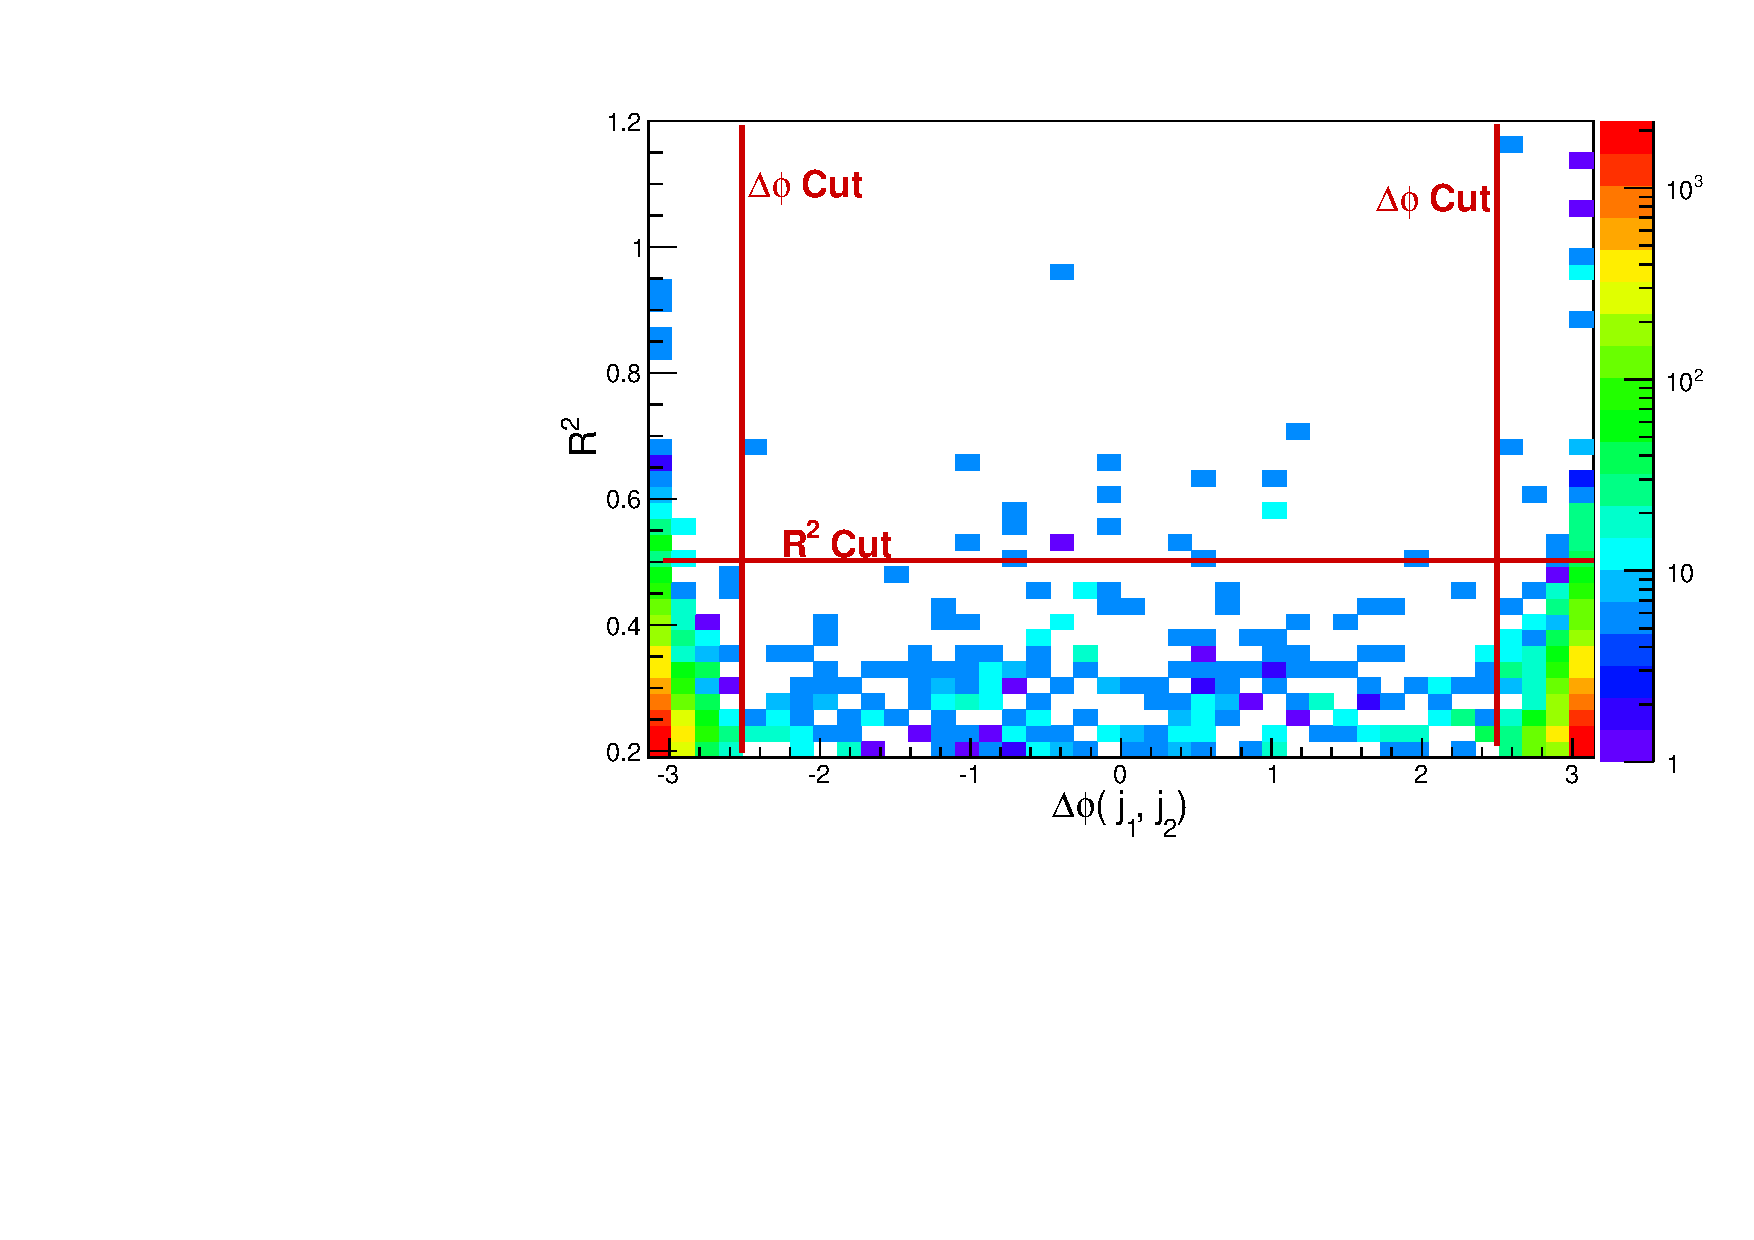
\includegraphics[trim = 2 0 0 0, clip = true,width=0.6\textwidth,angle=0.]{QCDplots/DPhi_R2_NoB_NoMu.pdf}\
\caption{ $\mathrm{R^2}$-$\Delta\phi  (J_{1}, J_{2})$ distribution for the QCD background in the $0\mu$ box.\label{dm:QCD2} }
\end{figure}
\begin{figure}[h]
\centering
\begin{tabular}{cc}
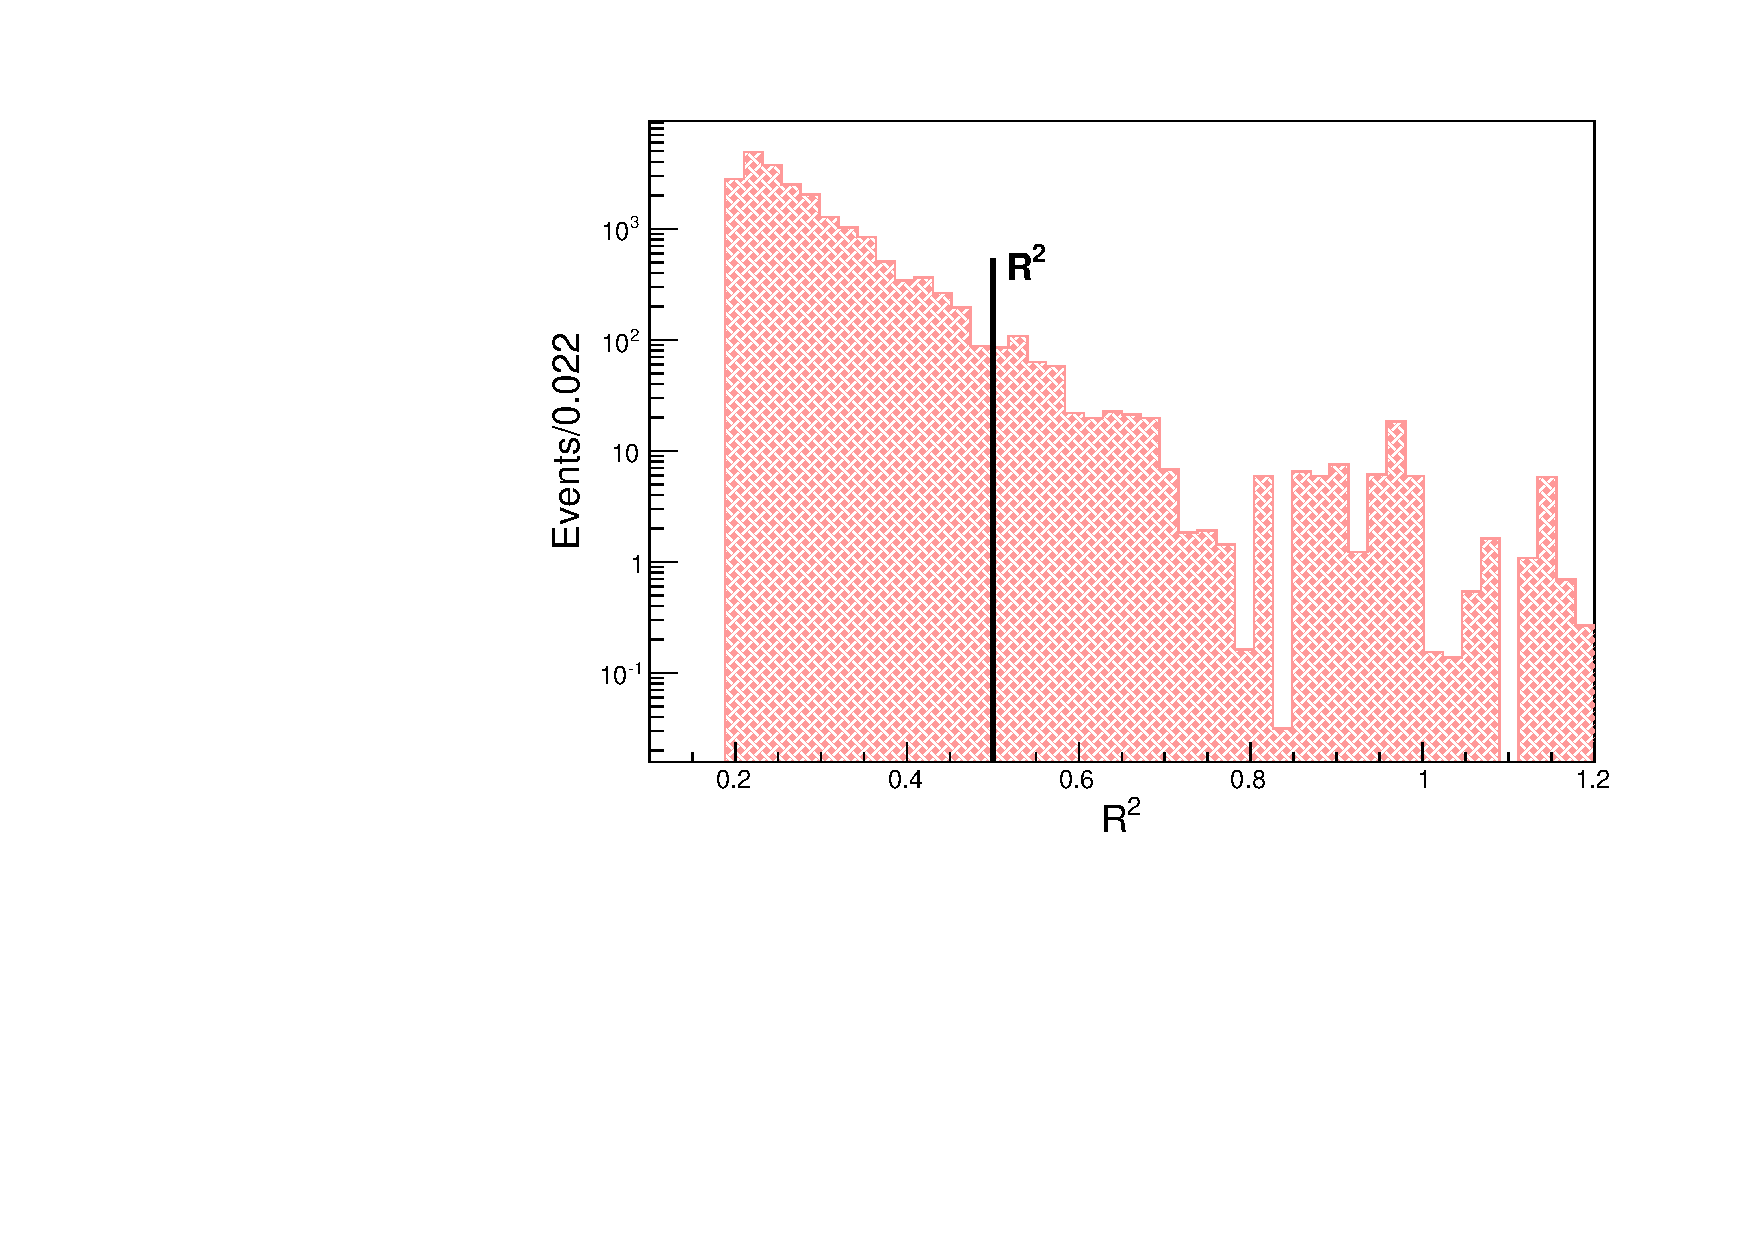
\includegraphics[trim = 2 0 0 0, clip = true, width=0.5\textwidth]{QCDplots/InclusiveR2_NoB_NoMu.pdf} &
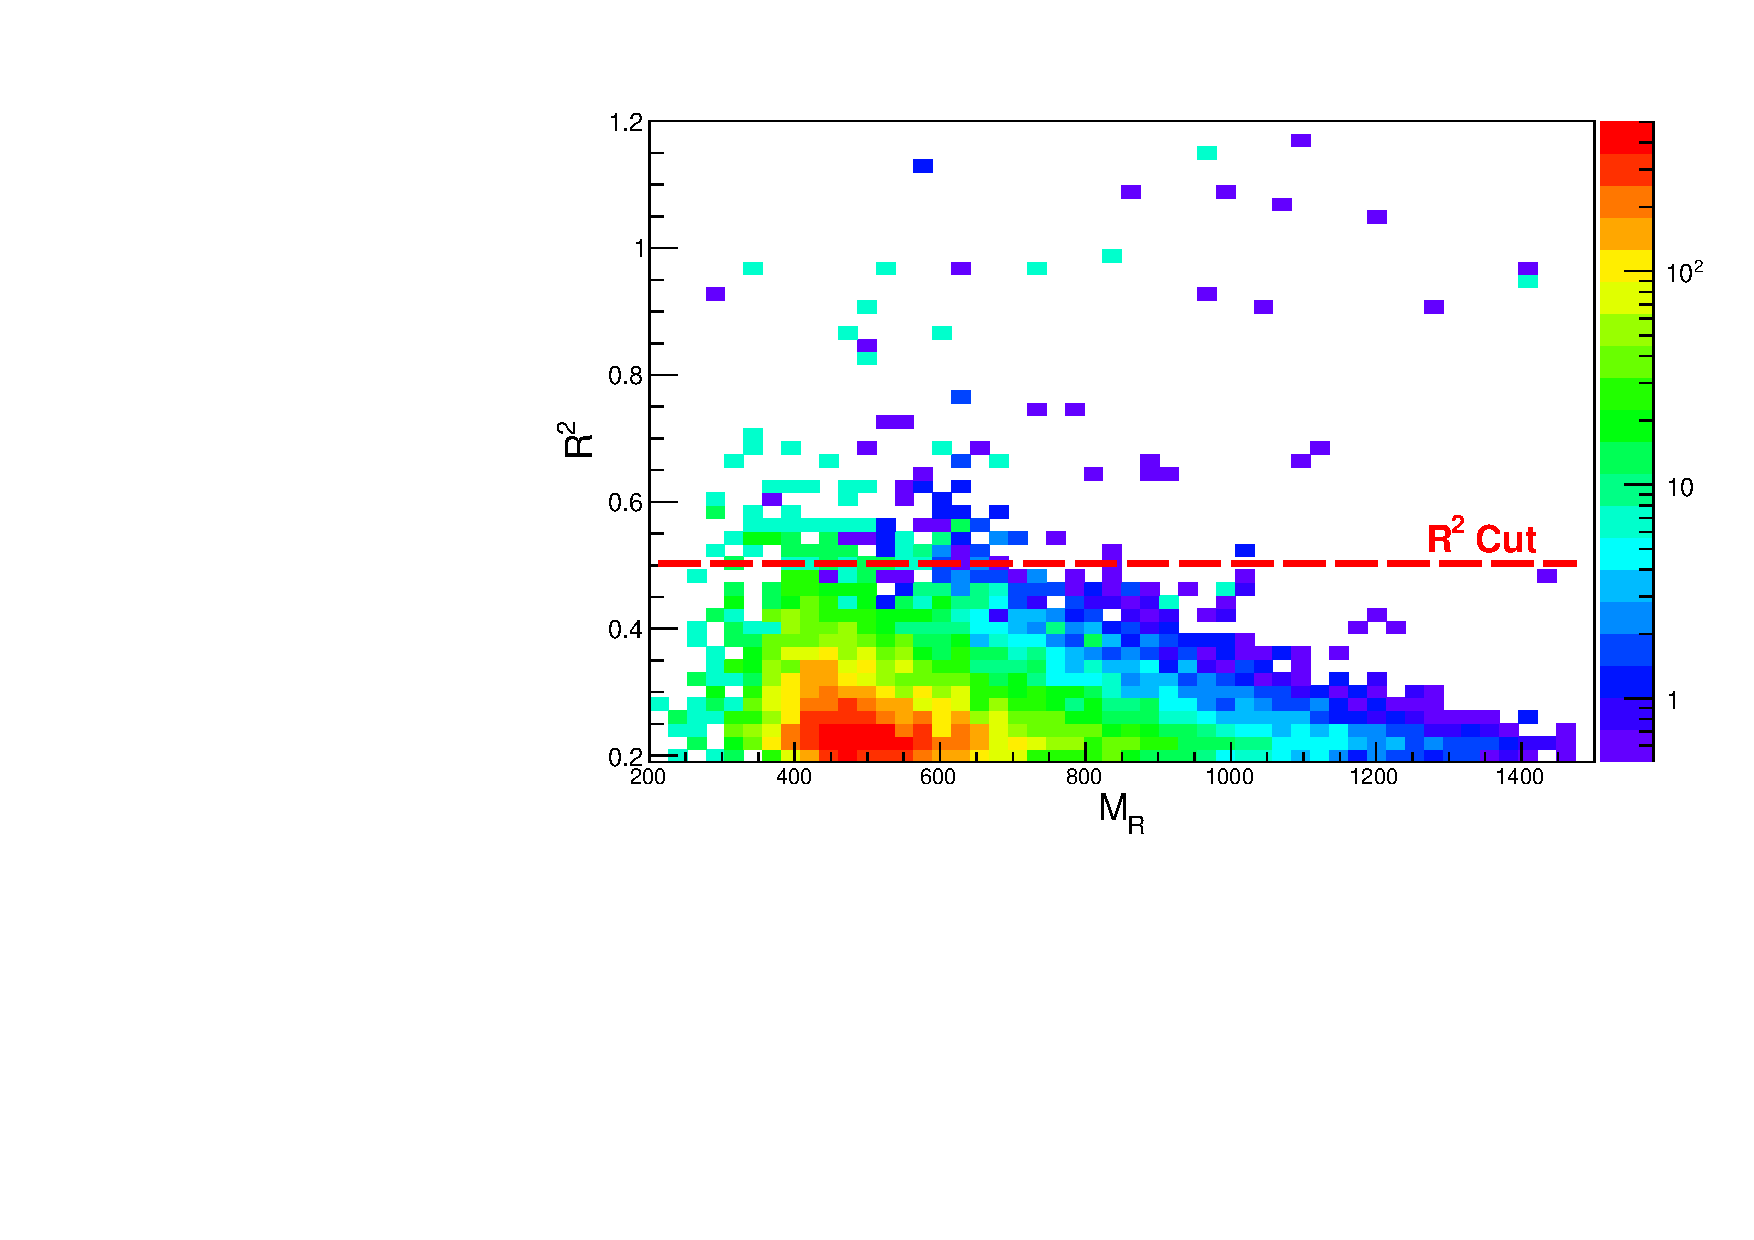
\includegraphics[trim = 2 0 0 0, clip = true, width=0.5\textwidth]{QCDplots/MR_R2_NoB_NoMu.pdf}\\
%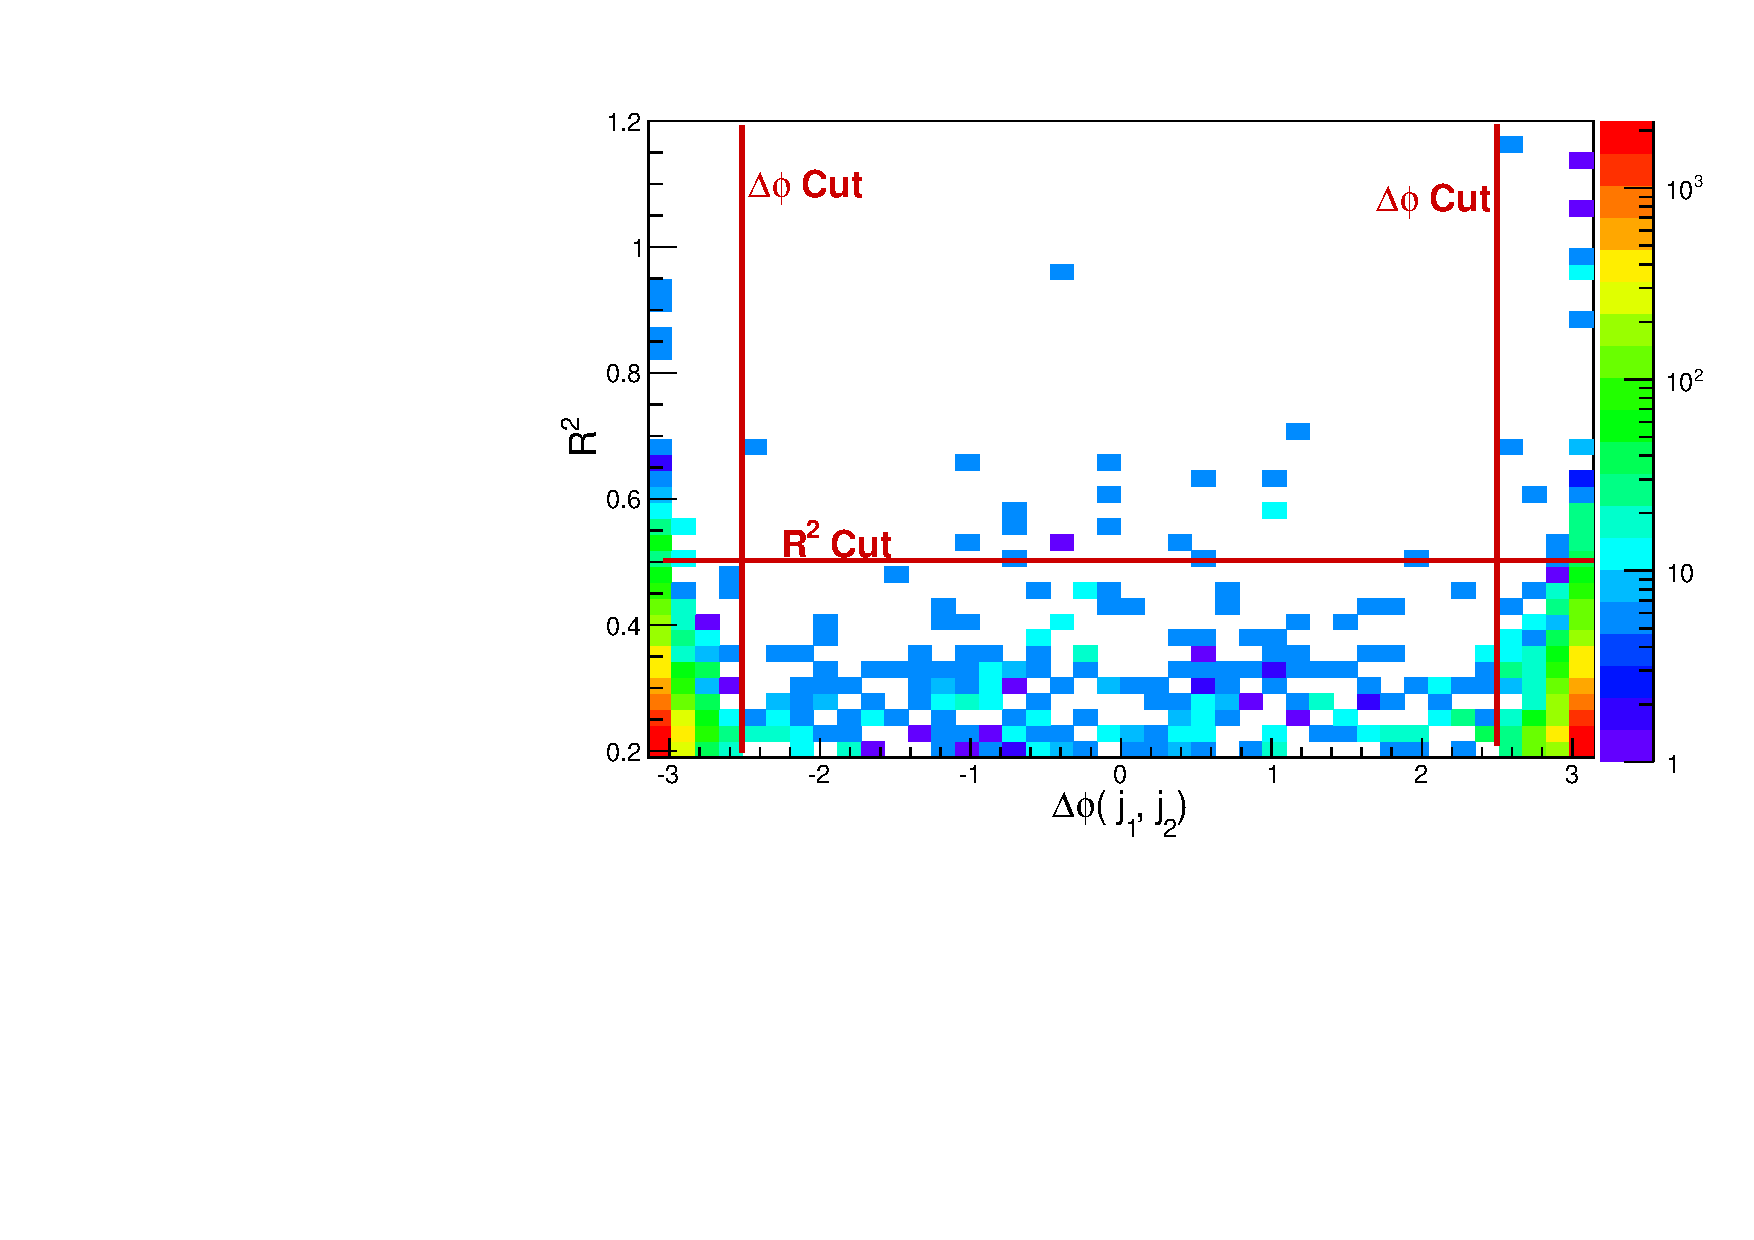
\includegraphics[trim = 2 0 0 0, clip = true,width=0.35\textwidth,angle=0.]{QCDplots/DPhi_R2_NoB_NoMu.pdf}\\
(a) & (b) \\
\end{tabular}
\caption{ (a) $\mathrm{R^2}$ and (b) $\mathrm{M_R}$-$\mathrm{R^2}$
  razor distributions for the QCD background in the $0\mu$ box.\label{dm:QCD1} }
\end{figure}

\subsection{Background estimation for the zero b-tag search region} 
\label{sec:bkgzmu}

To predict the background from $\PW(\ell\nu)$+jets and $\cPZ(\PGn\PAGn)$+jets in 
the zero b-tag search region, we use a data-driven method that extrapolates
the observed data yields in the 1$\mu$ control region to the search region.
Similarly, the observed yield in the 2$\mu$ control region allows the estimation of
the contribution from $\cPZ(\ell \ell)$+jets background process. Each
$\MR$ category is binned in $\RR^2$. 

The background expected from $\PW$ and $\cPZ$ boson production, in
each $\RR^2$ bin and in each $\MR$ category of the 0$\mu$
sample, is computed as
\begin{equation}
\footnotesize
  n_{i}^{0\mu} =  \Bigl(n_{i}^{1\mu} - N_{i}^{\ttbar,1\mu} - N_{i}^{\cPZ(\ell
    \ell)+\text{jets},1\mu}\Bigr) \frac{N_{i}^{\PW(\ell\nu)+\text{jets},0\mu}+N_{i}^{\cPZ(\PGn\PAGn)+\text{jets},0\mu}}{N_{i}^{\PW(\ell\nu)+\text{jets},1\mu}} +
\Bigl(n_{i}^{2\mu} - N_{i}^{\ttbar,2\mu}\Bigr) \frac{N_{i}^{\cPZ(\ell \ell)+\text{jets},0\mu}}{N_{i}^{\cPZ(\ell \ell)+\text{jets},2\mu}},
\label{eqn:pred}
\end{equation}
where $n_{i}^{k\mu}$ labels the data yield in bin $i$ for the sample
with $k$ muons, and $N_{i}^{X,k\mu}$ indicates the corresponding yield
for process $X$, derived from simulations. This background estimation method relies on 
the assumption that the kinematic properties of events in which $\PW$ and $\cPZ$ bosons are
produced are similar.

To estimate the accuracy of the background estimation method, we perform a cross-check 
by predicting the background in the 1$\mu$ control region using the observed data yield
in the 2$\mu$ control region. The Monte Carlo simulation is used to perform this extrapolation
analogous to the calculation in Equation~\ref{eqn:pred}.
The small contribution from the $\ttbar$ background process is also estimated using the simulated
samples. In Tables~\ref{tab:bkg1mu}~and~\ref{tab:bkg2mu}, the observed yields in the 1$\mu$ and 2$\mu$ control regions
respectively are compared to the estimate derived from data. In Tables~\ref{tab:bkg1mu}-\ref{tab:bkg0muWITHB}, 
the contribution of each process as predicted directly by simulated samples are also given.

\begin{table}[h]
  \topcaption{\label{tab:bkg1mu} Comparison of the observed yield in the
    1$\mu$ control region in each $\MR$ category and the
    corresponding data-driven background estimate obtained by extrapolating from the 2$\mu$ control region. The uncertainty in
    the estimates takes into account both the statistical
    and systematic components. The contribution of each individual background process is also shown, as
estimated from simulated samples, as well as the total MC predicted yield.}
\centering
\resizebox{\textwidth}{!}{
 \begin{tabular}{c*{6}{x}r}
   \hline
 \multicolumn{1}{c}{$\MR$ category} &  \multicolumn{1}{c}{$\cPZ(\PGn\PAGn)$+jets}  &  \multicolumn{1}{c}{$\PW(\ell
 \nu)$+jets}  &  \multicolumn{1}{c}{$\cPZ(\ell \ell)$+jets}  &  \multicolumn{1}{c}{$\ttbar$}  & \multicolumn{1}{c}{MC predicted}
 &\multicolumn{1}{c}{Estimated}  &  \multicolumn{1}{c}{Observed} \mT \mB\\
   \hline
   VL  &  0.7,0.3 & 4558,32 & 133,3 & 799,9 & 5491,33 & 5288,511 & 5926\mT\\
   L  &  0.5,0.3 & 1805,17 & 44,2 & 213,4 & 2063,18 & 1840,233 & 2110 \\
   H  &  0.1,0.1 & 915,11 & 16,1 & 66,2 & 997,11 & 629,240 & 923 \\
   VH  &   \multicolumn{1}{c}{$<$0.1}  & 183,5 & 2.6,0.2 & 8.5,0.8 & 194,5 & 166,93 & 143\mB\\
   \hline
 \end{tabular}
}
\end{table}

\begin{table}[h]
  \centering
  \topcaption{\label{tab:bkg2mu} Comparison of the observed yield for
    the 2$\mu$ control region in each $\MR$ category and the
    corresponding prediction from background simulation. The quoted uncertainty
    in the prediction reflects only the size of the simulated sample. The 
    contribution of each individual background process is also shown, as
    estimated from simulated samples.}
\resizebox{\textwidth}{!}{
 \begin{tabular}{*{6}{c}r}
   \hline
$\MR$  category&  $\cPZ(\PGn\PAGn)$+jets  &  $\PW(\ell
   \nu)$+jets  &  $\cPZ(\ell \ell)$+jets  &  $\ttbar$  &  MC predicted
   &  \multicolumn{1}{c}{Observed} \mT\mB\\
   \hline
   VL  &   $<$0.1  &  $<$0.1  & $214\pm4$ & $1.9\pm0.3$ & $215\pm4$ & 207\mT\\
   L  &    $<$0.1 & $0.4\pm0.3$ & $88\pm2$ & $0.5\pm0.2$ & $89\pm2$ & 78 \\
   H  &   $<$0.1  & $0.1\pm0.1$ & $48\pm1$ & $0.1\pm0.1$ & $48\pm1$ & 30 \\
   VH  &   $<$0.1  &  $<$0.1  & $10\pm1$ & $0.1\pm0.1$ & $10\pm1$ & 7\mB\\
   \hline
\end{tabular}
}
\end{table}

Figure~\ref{fig:1muCLOSURE} shows the comparison of the
$\RR^2$ distributions between the observed yield and the
data-driven background estimate in the 1$\mu$ control
region. The observed bin-by-bin difference is propagated as 
a systematic uncertainty in the data-driven background method,
and accounts for the statistical uncertainty in the 
event yield in the 2$\mu$ control region data as well as
potential differences in the modeling of the recoil spectra 
between $\PW$+jets and $\cPZ$+jets processes. Some bins exhibit 
relatively large uncertainties primarily due to statistical fluctuations
in the 2$\mu$ control region from which the background is prediction estimated. 
Though the uncertainties are rather large in fractional terms, 
sensitivity to DM signal models is still obtained, because of the enhanced 
signal to background ratio for the bins at large values of 
$\MR$ and $\RR^2$.



\begin{figure}
 \centering
   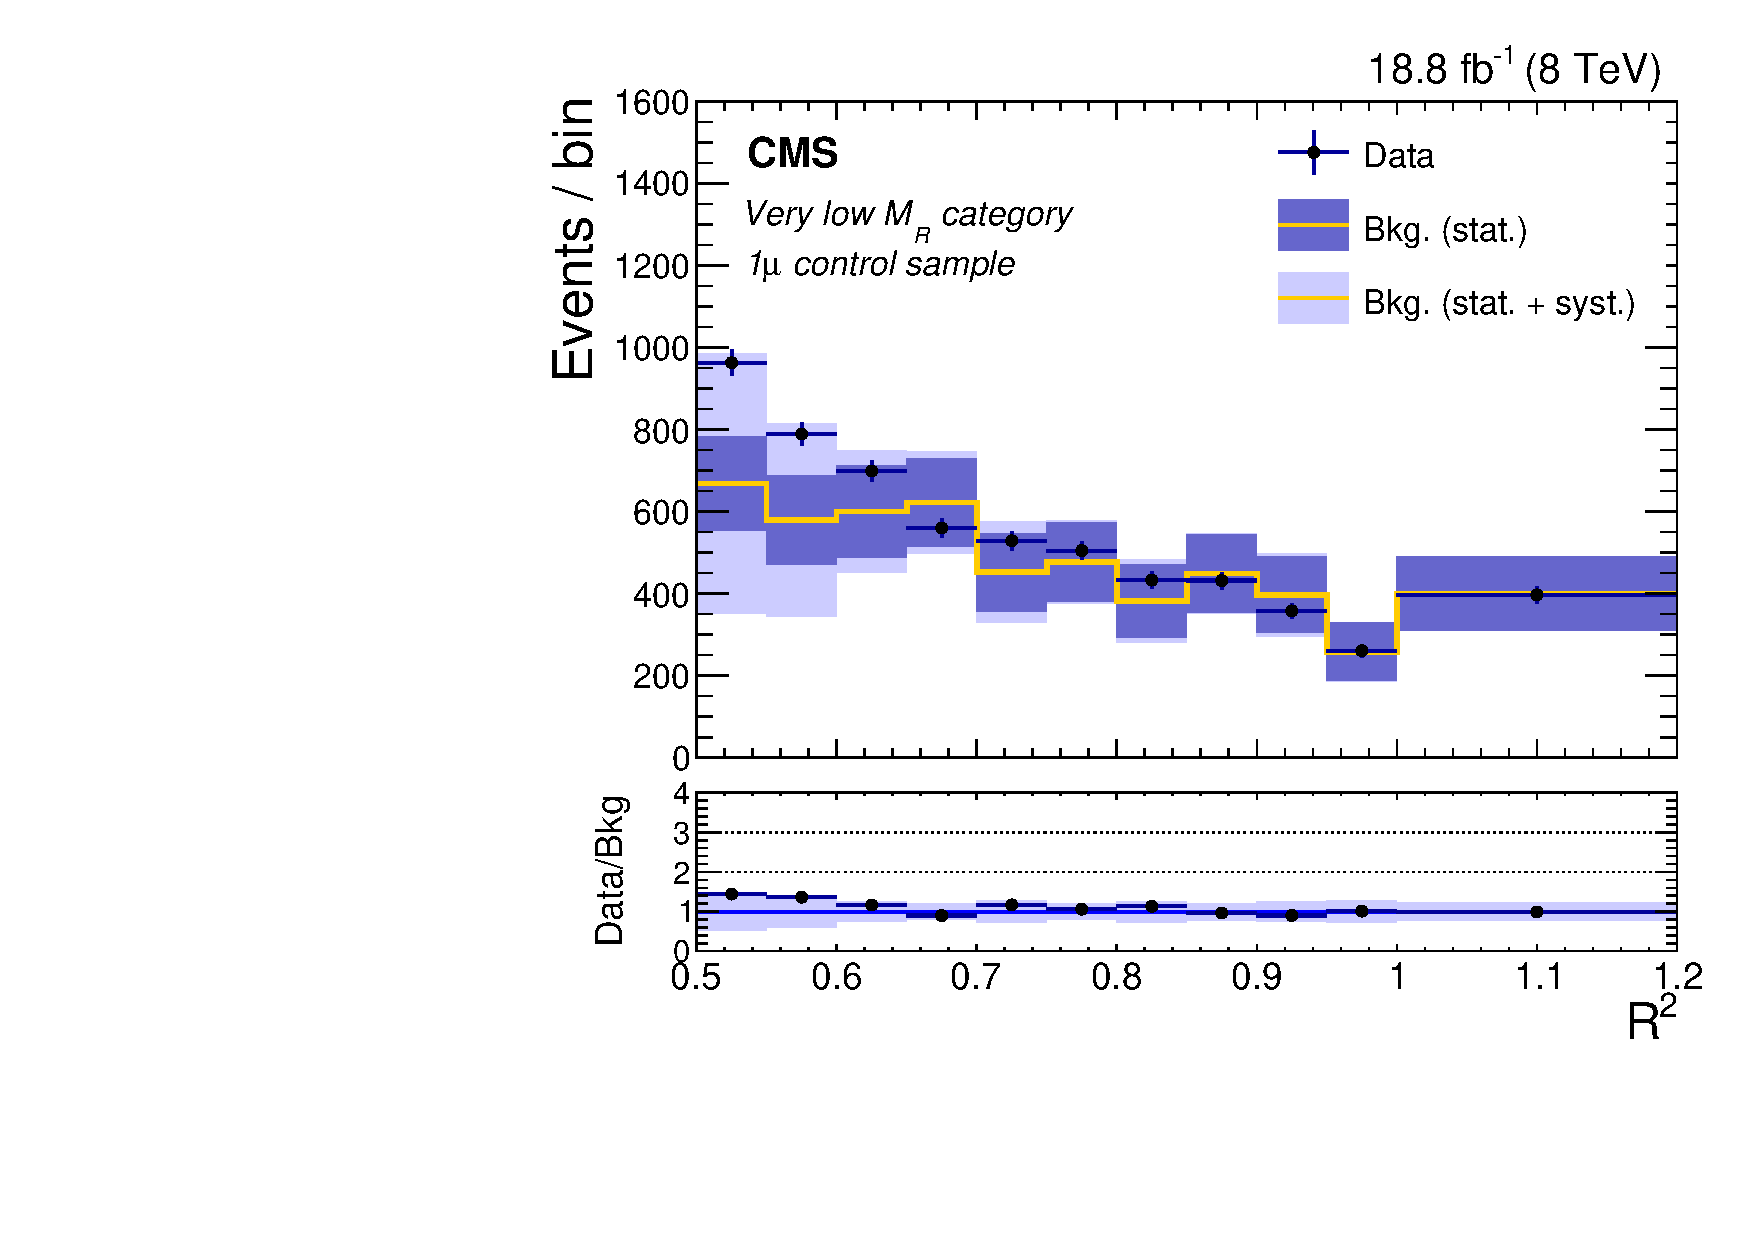
\includegraphics[width=0.48\textwidth]{PredPlotsAN_1MU_LE/OneMu_sys_cat_1.pdf}
   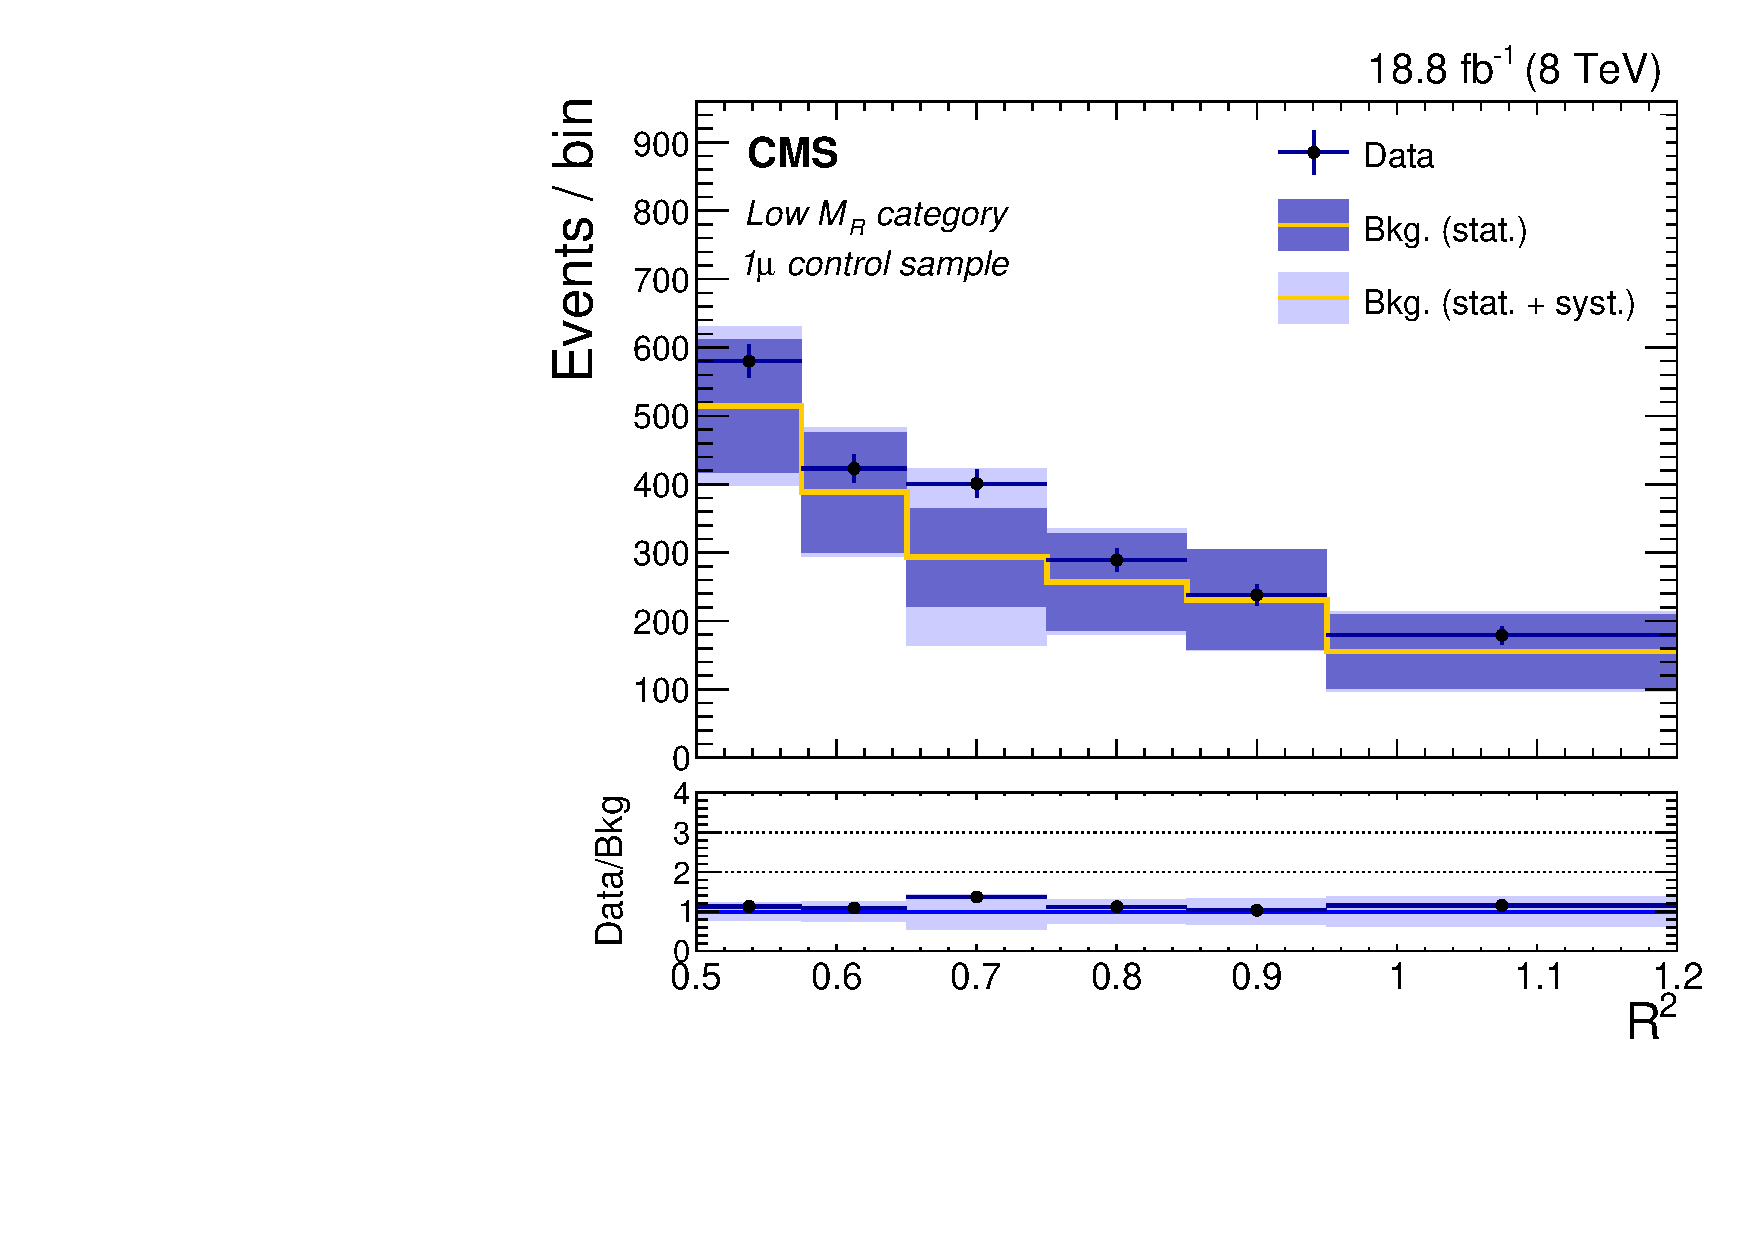
\includegraphics[width=0.48\textwidth]{PredPlotsAN_1MU_LE/OneMu_sys_cat_2.pdf}
   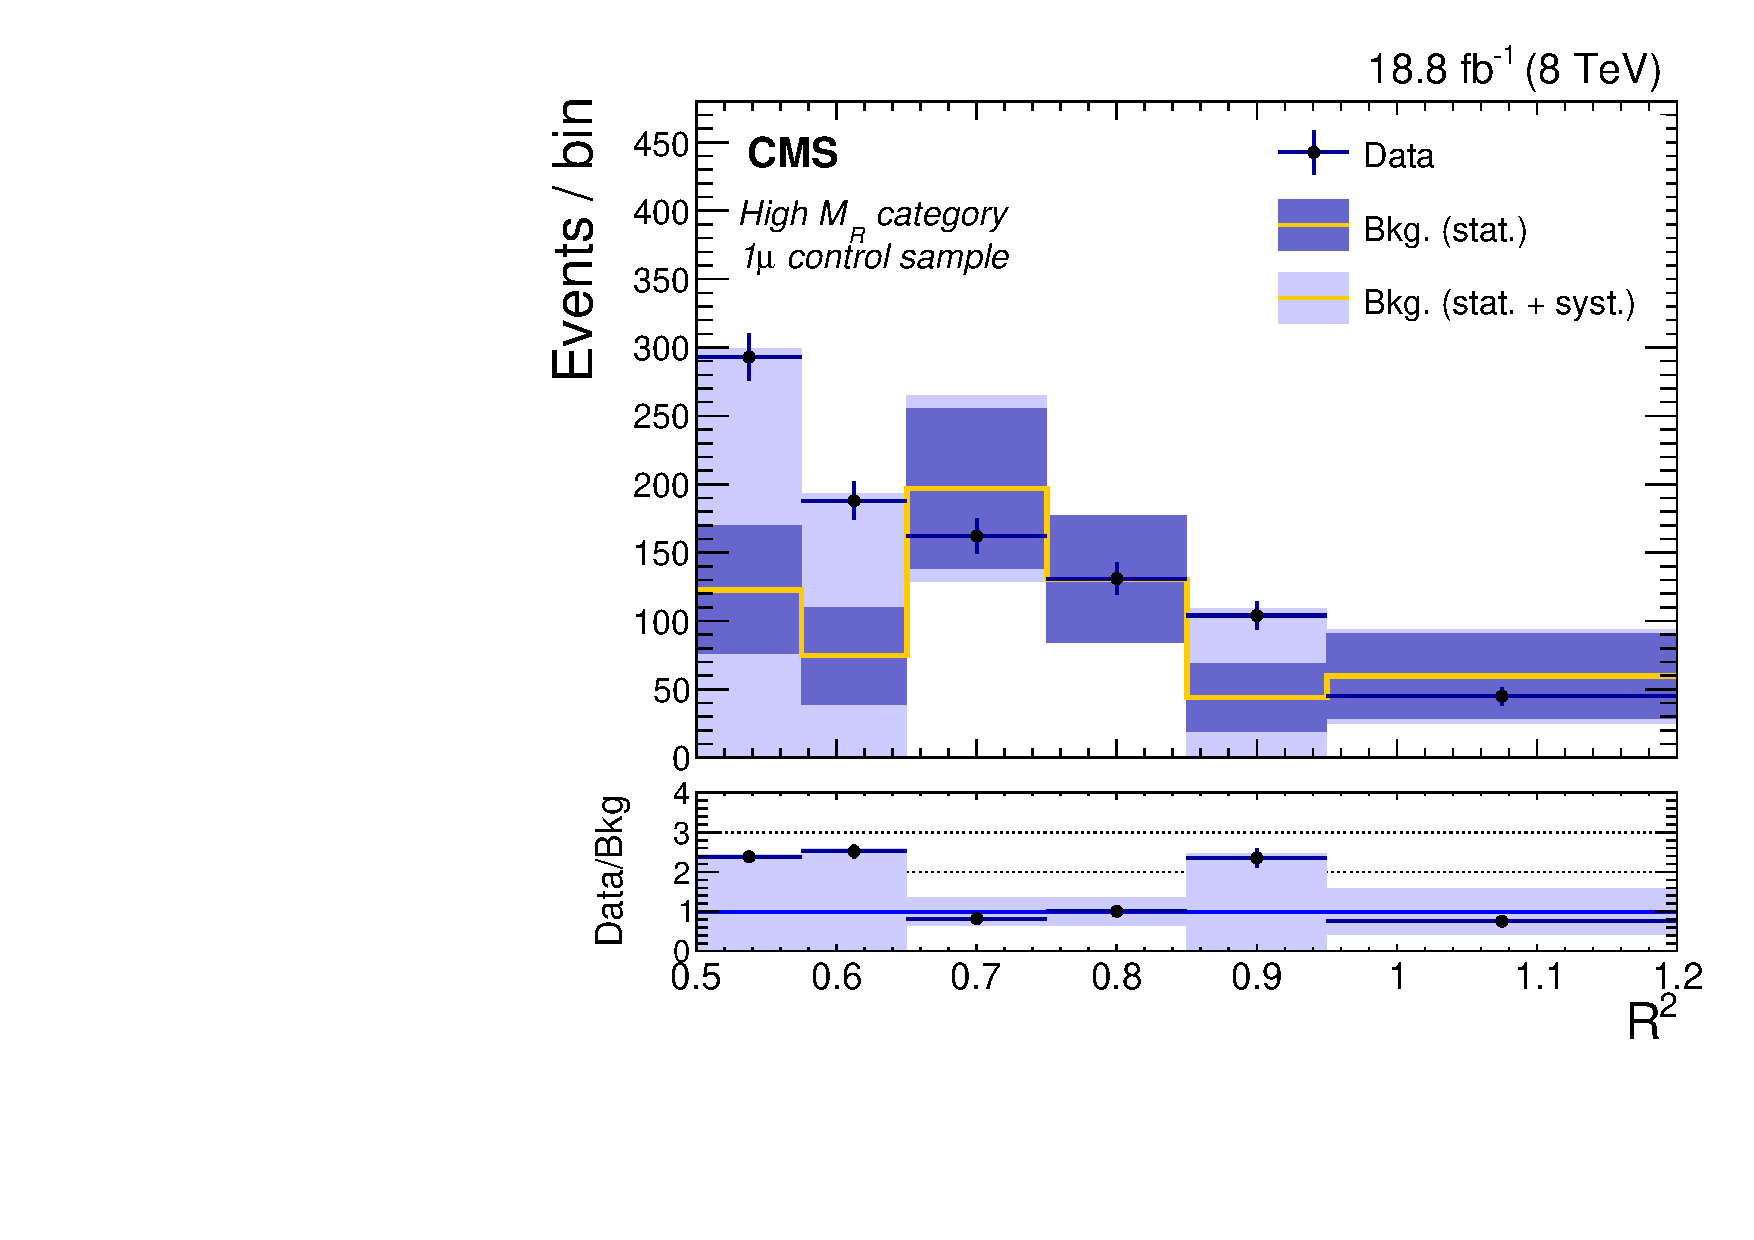
\includegraphics[width=0.48\textwidth]{PredPlotsAN_1MU_LE/OneMu_sys_cat_3.pdf}
   \includegraphics[width=0.48\textwidth]{PredPlotsAN_1MU_LE/OneMu_sys_cat_4.pdf}
 \caption{Comparison of observed yields in the 1$\mu$ control region and the
   data-driven background estimate derived from on the 2$\mu$ control region data in the four $\MR$ categories:
   VL (top left), L (top right), H (bottom left), and VH (bottom right). The bottom panel in each plot shows the
   ratio between the two distributions. The observed bin-by-bin
   deviation from unity is interpreted as an estimate of the systematic uncertainty
   associated to the background estimation methodology for the 0$\mu$ search region. The
   dark and light bands represent the statistical and the total
   uncertainties in the estimates, respectively. The horizontal bars indicate
the variable bin widths.\label{fig:1muCLOSURE}}
\end{figure}


The $\ttbar$ background is estimated using an analogous data-driven method,
where we derive corrections to the Monte Carlo simulation prediction
scaled to the $\ttbar$ production cross-section computed to NNLO accuracy~\cite{WatNNLO,ZatNNLO,TTbaratNNLO}
using data in the 2$\mu$b control region for each bin in $\RR^2$. 
The correction is then applied to the simulation prediction for
the $\ttbar$ background contribution to the zero b-tag search region.
This correction factor reflects potential mismodeling of the recoil
spectrum predicted by the Monte Carlo simulation. 
The contribution of each background process to
the 2$\mu$b sample, predicted from simulated samples, is given in
Table~\ref{tab:2mub}. The fraction of \ttbar events in the 2$\mu$b
control sample is ${\approx}95\%$. 
\begin{table}
\centering
\topcaption{\label{tab:2mub} Observed yield and predicted
    background from simulated samples in the 2$\mu$b control region.
    The quoted uncertainty in the prediction only reflects the size of the simulated sample. 
    The contribution of each individual background process is also shown,
    as estimated from simulated samples.}
\begin{tabular}{*{7}{c}}
  \hline
  Sample  &  $\cPZ(\PGn\PAGn)$+jets  &  $\PW(\ell \nu)$+jets &
  $\cPZ(\ell \ell)$+jets  &  $\ttbar$  & MC predicted &  Observed \mT\mB\\
  \hline
  2$\mu$b  &   $<$0.1  & $0.1\pm0.1$ & $2.2\pm0.3$ & $58\pm2$ & $60\pm2$ & 60 \mT\mB\\
  \hline
\end{tabular}
\end{table}
Figure~\ref{fig:2mub} shows the comparison of the observed
yield and the prediction from simulation, as a function of
$\RR^2$. We observe no significant deviations between the observed
data and the simulation prediction. The uncertainty derived from the 
data-to-simulation correction factor is propagated to the systematic uncertainty 
of the $\ttbar$ prediction in the zero b-tag search region. 

\begin{figure}
  \centering
   \includegraphics[width=0.47\textwidth]{BtagPlots/MC_CP_2Mu1TbTT_Sep.pdf}
   \caption{Comparison of the observed yield and the prediction from
     simulation as a function of $\RR^2$ in the 2$\mu$b control region.
     The uncertainties in the data and the simulated
     sample are represented by the vertical bars and the shaded bands,
     respectively. The horizontal bars indicate
the variable bin widths.\label{fig:2mub}}
\end{figure}
The result of the background estimation in the zero b-tag search region is given in
Table~\ref{tab:bkg0mu}, where it is compared to the observed yields in
data. The uncertainty in the background estimates takes into account
both the statistical and systematic components.
%The contribution of each process is also given,
%as predicted directly by simulated samples and therefore not used in
%the final result.
\begin{table}
\centering
\topcaption{\label{tab:bkg0mu}  Comparison of the observed yields for
  for the zero b-tag search region in each $\MR$ category and the
   corresponding background estimates. The uncertainty in
    the background estimate takes into account both the statistical
    and systematic components. The contribution of each individual background process is also shown, as
estimated from simulated samples, as well as the total MC predicted yield.}
\resizebox{\textwidth}{!}{
 \begin{tabular}{c*{6}{x}r}
  \hline
\multicolumn{1}{c}{$\MR$ category} &  \multicolumn{1}{c}{$\cPZ(\PGn\PAGn)$+jets}  &  \multicolumn{1}{c}{$\PW(\ell \nu)$+jets}  &  \multicolumn{1}{c}{$\cPZ(\ell \ell)$+jets}  &  \multicolumn{1}{c}{$\ttbar$}  & \multicolumn{1}{c}{MC predicted}&  \multicolumn{1}{c}{Estimated}  &  \multicolumn{1}{c}{Observed} \mT\mB\\
  \hline
  VL  &  6231,37  & 4820,33 & 49,2 & 555,7 & 11655,50 &12770,900 & 11623 \mT\\
  L  &  2416,19 & 1513,16 & 11,1 & 104,3 & 4044,25 & 4170,270 & 3785 \\
  H  &  1127,7 & 625,9 & 2.9,0.3 & 24,1  &  1779,12 & 1650,690 & 1559 \\
  VH  &  229,2 & 103,3 & 0.2,0.1 & 3.1,0.5 &
   335,3 & 240,160 & 261\mB\\
  \hline
\end{tabular}
}
\end{table}
The comparison of the data-driven background estimates and the observations for
each $\MR$ category is shown in Fig.~\ref{fig:0muSignalBkg1GeV}, as a function of $\RR^2$. 
The expected event distribution is shown for two signal
benchmark models, corresponding to the pair production of DM particles
of mass 1\GeV in the effective field theory (EFT) approach with vector coupling to u or d quarks. 
Details on the signal benchmark models are given in Section~\ref{sec:EFT0mu}.
\begin{figure}
 \centering
   \includegraphics[width=0.48\textwidth]{SignalBkgPlots/Data_MC_cat1_1_DoubleSignal_V.pdf}
   \includegraphics[width=0.48\textwidth]{SignalBkgPlots/Data_MC_cat2_1_DoubleSignal_V.pdf}
   \includegraphics[width=0.48\textwidth]{SignalBkgPlots/Data_MC_cat3_1_DoubleSignal_V.pdf}
   \includegraphics[width=0.48\textwidth]{SignalBkgPlots/Data_MC_cat4_1_DoubleSignal_V.pdf}
 \caption{Comparison of the observed yield in the zero b-tag control region and the
   background estimates in the four $\MR$ categories:
   VL (top left), L (top right), H (bottom left), and VH (bottom right). The
   contribution of individual background processes is shown by the
   filled histograms. The bottom panels show the ratio
   between the observed yields and the total background estimate. For reference, the distributions from two
   benchmark signal models are also shown, corresponding to the pair
   production of DM particles of mass 1\GeV in the EFT approach with
   vector coupling to u or d quarks. The horizontal bars indicate
the variable bin widths.\label{fig:0muSignalBkg1GeV} }
\end{figure}


\subsection{Background estimation for the \texorpdfstring{0$\mu$b and 0$\mu$bb}{0 mu b and 0 mu bb} samples}

A similar data-driven technique is used to determine the expected background for the 
one and two b-tag search regions. The background from $\ttbar$ events for each $\RR^2$ bin in the
one b-tag search region, $n(\ttbar)_{i}^{0\mu\PQb}$, is computed as:
\begin{equation}
  n(\ttbar)_{i}^{0\mu\PQb} =  \bigl(n(\ttbar)_{i}^{2\mu\PQb} - N_{i}^{\cPZ(\ell
    \ell)+\text{jets},2\mu\PQb} - N_{i}^{\PW(\ell\nu)+\text{jets},2\mu\PQb}\bigr)
\frac{N(\ttbar)_{i}^{0\mu\PQb}}{N(\ttbar)_{i}^{2\mu\PQb}}\label{eq:bBkgPred}
\end{equation}
where $n(\ttbar)_{i}^{2\mu\PQb}$ is the observed yield in the $i$th $\RR^2$
bin in the 2$\mu$b control region, while $N(\ttbar)_{i}^{0\mu\PQb}$ and
$N(\ttbar)_{i}^{2\mu\PQb}$ are the $\ttbar$ yields in the $i$th $\RR^2$ bin 
predicted by the simulation for the one b-tag search region and the 2$\mu$b control region
respectively. Similarly, the \ttbar background in the two b-tag search region
is derived from Eq.~(\ref{eq:bBkgPred}), replacing $N(\ttbar)_{i}^{0\mu\PQb}$ 
with $N(\ttbar)_{i}^{0\mu\mathrm{bb}}$, the \ttbar
background yield in the $i$th bin of the two b-tag search region predicted
by the simulation. The data yield in the 2$\mu$b control region is
corrected to account for the small contamination from $\cPZ$+jets and
$\PW$+jets, predicted with the simulated yields $N_{i}^{\cPZ(\ell\ell)+\text{jets},2\mu\PQb}$ and
$N_{i}^{\PW(\ell\nu)+\text{jets},2\mu\PQb}$, respectively.


The background contribution from $\PW(\ell \nu)$+jets and $\cPZ(\PGn\PAGn)$+jets events is 
predicted using the $\cPZ(\mu\mu)$b control region, and summarized in Table~\ref{tab:WITHB}.
The $\cPZ$+jets purity of this control region is ${\approx}$89\%. 
The observed yield in the $\cPZ(\mu\mu)$b control region is shown in the left plot of Fig.~\ref{fig:Zmumub}, 
as a function of $\RR^2$, along with the Monte Carlo simulation prediction. The uncertainty on the
simulation prediction accounts only for the statistical uncertainty of the simulated sample.
This contribution, scaled by the ratio of the predicted V+jets background in the search regions 
to that in the control region, obtained from simulation, provides an estimate for each $\RR^2$ bin. 

\begin{table}
\centering
\topcaption{\label{tab:WITHB}
    Comparison of the observed yields in the $\cPZ(\mu\mu)$b and
    $1\mu$b samples, the corresponding predictions from background
    simulation, and (for $1\mu$b only) the cross-check background
    estimate. The contribution of each individual background process is also shown, as
estimated from simulated samples.}
\resizebox{\textwidth}{!}{
\begin{tabular}{*{7}{c}r}
  \hline
  Sample  &  $\cPZ(\PGn\PAGn)$+jets  &  $\PW(\ell \nu)$+jets  &
  $\cPZ(\ell \ell)$+jets  &  $\ttbar$   &  MC predicted  & Estimated &
  \multicolumn{1}{c}{Observed} \mT\mB\\
  \hline
   $\cPZ(\mu\mu)$b  &  $<$0.1  &  $<$0.1  & $134\pm3$ & $17\pm1$ &
   $151\pm3$ &\NA  &  175 \mT\mB\\
   $1\mu$b &  $0.2\pm0.1$ & $279\pm7$ & $11\pm1$ & 3038 $\pm$
   17 & $3328\pm18$ & $3410\pm540$ & 2920\mT\mB\\
  \hline
\end{tabular}
}
\end{table}
\begin{figure}
\centering
   \includegraphics[width=0.48\textwidth]{BtagPlots/MC_CP_2Mu1LbZ_Sep.pdf}
   \includegraphics[width=0.48\textwidth]{BtagPlots/Closure_CP_1mu1Tb_SYS_Sep.pdf}
 \caption{Comparison of the observed yield and the
   prediction from simulation in the $\cPZ(\mu\mu)$b control sample (left)
   and of the observed yield in the $1\mu$b control sample and
   the background estimates from the 2$\mu$b and $\cPZ(\mu\mu)$b
   control samples (right), shown as a function of $\RR^2$. The bottom
   panel of each figure shows the ratio between the data and the
   estimates. The shaded bands represent the statistical uncertainty
   in the left plot, and the total uncertainty in the right plot. The horizontal bars indicate
the variable bin widths.\label{fig:Zmumub}}
\end{figure}

We perform a cross-check of the method on the 1$\mu$b control region
by predicting the background from the 2$\mu$b control region data.
The data and prediction are compared on the right of Fig.~\ref{fig:Zmumub},
where we observe reasonable agreement. The difference between the 
prediction and the observed data in this cross-check region is propagated as a
systematic uncertainty of the method. 

The estimated background in the one and two b-tag search regions
is given in Table~\ref{tab:bkg0muWITHB} and shown in Fig.~\ref{fig:0muttbar}, where it is compared to
the observed yields in data. The uncertainty in the
estimates take into account both the statistical and systematic
components.% In the table, the yield expected from simulation is
\begin{figure}
   \includegraphics[width=0.48\textwidth]{BtagPlots/Bkg_0mu2TbEXC_CP.pdf}
   \includegraphics[width=0.48\textwidth]{BtagPlots/Bkg_0mu1TbEXC_CP.pdf}
 \caption{Comparison of observed event yields and background
   estimates as a function of $\RR^2$, for the
   one (left) and two (right) b-tag search regions.
   The shaded bands represent the total uncertainty in the estimate. The horizontal bars indicate
the variable bin widths.\label{fig:0muttbar}}
\end{figure}
\begin{table}
\centering
  \topcaption{ Comparison of the observed yield for
    events in the one and two b-tag search regions and the corresponding background
    estimates. The uncertainty in the estimates takes into account
    both the statistical and systematic components. The contribution of each individual background process is also shown, as
estimated from simulated samples, as well as the total MC predicted yield.
\label{tab:bkg0muWITHB}}
\resizebox{\textwidth}{!}{
\begin{tabular}{*{7}{c}r}
  \hline
 Sample  &  $\cPZ(\PGn\PAGn)$+jets  &  $\PW(\ell \nu)$+jets  &
  $\cPZ(\ell \ell)$+jets  &  $\ttbar$  & MC predicted& Estimated &  \multicolumn{1}{c}{Observed} \mT\mB\\
\hline
  $0\mu$bb  &  $44\pm3$  &  $14\pm2$  &  $0.2\pm0.1$  &  204
  $\pm$ 4  & $262\pm5$ &  $271\pm37$  &  247 \mT\mB\\
  $0\mu$b  &  $417\pm8$  &  $216\pm7$  &  $2.4\pm0.4$  &  $1480\pm12$  & $2115\pm16$ &  $2230\pm280$  &  2282 \mT\mB\\
\hline
\end{tabular}
}
\end{table}




\section{Systematic uncertainties}\label{sec:sys}

For each $\RR^2$ bin in each $\MR$ category, the
difference between the observed and estimated yields in the
crosscheck analysis (see Section~\ref{sec:bkg}) is taken as the estimate of the uncertainty associated with the
method. The uncertainty is found to
be typically ${\approx}$20--40\%, depending on the considered bin in the
($\MR$, $\RR^2$) plane. Other sources of systematic uncertainties such
as the modeling of the jet energy scale correction, and the initial-state
radiation in the event are found to be negligible compared to the
systematic from the
cross-check. Figures~\ref{dm:ccJES} and ~\ref{dm:ccISR} show the indiviual systematic uncertaintes just
mentioned and the systematic uncertainty from the cross-check.

\begin{figure}[ht!]
 \centering
 \begin{tabular}{cccc}
   \includegraphics[width=0.4\textwidth]{SysPlots/cat1_JES.pdf}&
   \includegraphics[width=0.4\textwidth]{SysPlots/cat2_JES.pdf}\\
   (a) & (b)\\
   \includegraphics[width=0.4\textwidth]{SysPlots/cat3_JES.pdf}&
   \includegraphics[width=0.4\textwidth]{SysPlots/cat4_JES.pdf}\\
   (c) & (d)\\
 \end{tabular}
 \caption{Total (estimated using the cross-check analysis) and JES
   systematic uncertainties. The green band corresponds to the
   systematic uncertainty associated with the background prediction
   method, while the red band corresponds to the JES systematic only. Panels (a) and (b) show the VL and L $\mathrm{M_{R}}$
   categories, respectively. Panels (c) and (d) show the H and VH $\mathrm{M_{R}}$
   categories, respectively.\label{dm:ccJES}}
\end{figure}
\begin{figure}[ht!]
 \centering
 \begin{tabular}{cc}
   \includegraphics[width=0.4\textwidth]{SysPlots/cat1_ISR.pdf}&
   \includegraphics[width=0.4\textwidth]{SysPlots/cat2_ISR.pdf}\\
   (a) & (b)\\
   \includegraphics[width=0.4\textwidth]{SysPlots/cat3_ISR.pdf}&
   \includegraphics[width=0.4\textwidth]{SysPlots/cat4_ISR.pdf}\\
   (c) & (d)\\
 \end{tabular}
 \caption{Total (estimated using the cross-check analysis) and ISR
   systematic uncertainties. The green band corresponds to the
   systematic uncertainty associated with the background prediction
   method, while the red band corresponds to the ISR systematic
   only. Panels (a) and (b) show the VL and L $\mathrm{M_{R}}$
   categories, respectively. Panels (c) and (d) show the H and VH $\mathrm{M_{R}}$
   categories, respectively.\label{dm:ccISR}}
\end{figure}

The largest systematic uncertainty arises from the crosscheck
analysis. This uncertainty is affected by statistical
fluctuations from the limited number of selected events in the 2$\mu$
control region. This uncertainty covers the differences
in the modeling of the recoil spectra between $\PW$+jets and $\cPZ$+jets processes as well as
the cross section uncertainties.

For the 0$\mu$ analysis, differences between the kinematic properties of $\PW$+jets and
$\cPZ$+jets events are additional sources of systematic uncertainty. These
differences arise from the choice of the PDF set, jet energy scale
corrections, b tagging efficiency
corrections, and trigger efficiency. These effects largely cancel when taking the ratio of the two processes, and the resulting
uncertainty is found to be smaller than one fifth
of the total uncertainty.  The quoted uncertainty is an upper
estimate of the total systematic uncertainty.

For the 0$\mu$b and 0$\mu$bb samples, both the signal and control samples are dominated by \ttbar events. The cancellation of the
systematic uncertainties is even stronger in
this case, since it does not involve different processes, and different
PDFs. The remaining uncertainty is
dominated by the contribution arising from the small size of the control
sample.

Systematic uncertainties in the signal simulation
originate from the choice of the PDF set,
the jet energy scale correction, the modeling of the initial-state radiation in the event
generator, and the uncertainty in the integrated luminosity. The
luminosity uncertainty changes the signal normalization while the other
uncertainties also modify the signal shape.
These effects are taken into account by propagating these
uncertainties into the $\MR$ category and the $\RR^2$
bin. Figures~\ref{dm:signalPDF}, ~\ref{dm:signalJES}, and
~\ref{dm:signalISR} show the PDF,
jet energy scale, and the initial-state radiation systematic
uncertainties for a vector-mediated EFT signal model with DM mass of 700\GeV, respectively. These uncertainties are
considered to be fully correlated across $\MR$ categories and
$\RR^2$ bins. Typical values for the individual contributions
are given in Table~\ref{tab:sygSys}. The total uncertainty in the
signal yield is obtained by propagating the individual effects into
the $\MR$ and $\RR^2$ variables and comparing the bin-by-bin variations with respect to the central value of the prediction
based on simulation. In the particular case of the uncertainties due
to the choice of the PDF set we have followed the PDF4LHC~\cite{Bourilkov:2006cj,Alekhin:2011sk,Botje:2011sn} prescription, using the CTEQ-6.6\cite{Nadolsky:2008zw} and MRST-2006-NNLO~\cite{Martin:2007bv} PDF sets.

\begin{figure}[ht!]
 \centering
 \begin{tabular}{cc}
   \includegraphics[width=0.4\textwidth]{SysPlots/DMm700Vu_PDF_cat1.pdf}&
   \includegraphics[width=0.4\textwidth]{SysPlots/DMm700Vu_PDF_cat2.pdf}\\
   (a) & (b)\\
   \includegraphics[width=0.4\textwidth]{SysPlots/DMm700Vu_PDF_cat3.pdf}&
   \includegraphics[width=0.4\textwidth]{SysPlots/DMm700Vu_PDF_cat4.pdf}\\
   (c) & (d)\\
 \end{tabular}
 \caption{PDF systematic uncertainty for a vector mediated EFT signal
   model with DM mass = 700\GeV. The blue band corresponds to the
   systematic error associated with PDF uncertainty. Panels (a) and (b) show the VL and L $\mathrm{M_{R}}$
   categories, respectively. Panels (c) and (d) show the H and VH $\mathrm{M_{R}}$
   categories, respectively.\label{dm:signalPDF}}
\end{figure}
\begin{figure}[ht!]
 \centering
 \begin{tabular}{cccc}
   \includegraphics[width=0.4\textwidth]{SysPlots/DMm700Vu_JES_cat1.pdf}&
   \includegraphics[width=0.4\textwidth]{SysPlots/DMm700Vu_JES_cat2.pdf}\\
   (a) & (b)\\
   \includegraphics[width=0.4\textwidth]{SysPlots/DMm700Vu_JES_cat3.pdf}&
   \includegraphics[width=0.4\textwidth]{SysPlots/DMm700Vu_JES_cat4.pdf}\\
   (c) & (d)\\
 \end{tabular}
 \caption{JES systematic uncertainty for a vector mediated EFT signal
   model with DM mass = 700\GeV. The blue band corresponds to the
   systematic error associated with JES uncertainty. Panels (a) and (b) show the VL and L $\mathrm{M_{R}}$
   categories, respectively. Panels (c) and (d) show the H and VH $\mathrm{M_{R}}$
   categories, respectively.\label{dm:signalJES}}
\end{figure}
\begin{figure}[ht!]
 \centering
 \begin{tabular}{cccc}
   \includegraphics[width=0.4\textwidth]{SysPlots/DMm700Vu_ISR_cat1.pdf}&
   \includegraphics[width=0.4\textwidth]{SysPlots/DMm700Vu_ISR_cat2.pdf}\\
   (a) & (b)\\
   \includegraphics[width=0.4\textwidth]{SysPlots/DMm700Vu_ISR_cat3.pdf}&
   \includegraphics[width=0.4\textwidth]{SysPlots/DMm700Vu_ISR_cat4.pdf}\\
   (c) & (d)\\
 \end{tabular}
 \caption{ISR systematic uncertainty for a vector mediated EFT signal
   model with DM mass = 700\GeV. The blue band corresponds to the
   systematic error associated with ISR uncertainty. Panels (a) and (b) show the VL and L $\mathrm{M_{R}}$
   categories, respectively. Panels (c) and (d) show the H and VH $\mathrm{M_{R}}$
   categories, respectively.\label{dm:signalISR}}
\end{figure}

\begin{table}
 \centering
 \topcaption{\label{tab:sygSys} Systematic uncertainties associated with
  the description of the DM signal. The values indicated represent
  the typical size. The dependence of these systematic uncertainties on
  the $\RR^2$ and $\MR$ values is taken into
  account in the determination of the results.}
 \begin{tabular}{ll}
  \hline
  \multicolumn{1}{c}{Effect}  &  \multicolumn{1}{c}{Uncertainty}\\
  \hline
  Jet energy scale  &  3--6\%\\
  Luminosity  &  2.6\%\\
  Parton distribution functions  &  3--6\%\\
  Initial-state radiation  &  8--15\%\\
  \hline
\end{tabular}
\end{table}

\section{Results and interpretation}\label{sec:interpretation}

In Figs.~\ref{fig:0muSignalBkg1GeV}~and~\ref{fig:0muttbar} the
estimated backgrounds are compared to the observed yield in each
$\MR$ region, for events without and with
b-tagged jets, respectively. The background estimates agree with the observed
yields, within the uncertainties. This result is interpreted in terms of exclusion limits
for several models of DM production.



\subsection{Limits on dark matter production from the \texorpdfstring{0$\mu$}{0 mu} sample}\label{0muResults}
\label{sec:EFT0mu}
The result is interpreted in the context of a low-energy effective
field theory, in which
the production of DM particles is mediated by six or seven dimension
operators~\cite{maverickDM,TevatronDMFrontier}. This choice allows
the results be compared with those of previous
analyses~\cite{Aad:2011xw,Chatrchyan:2012me},
and shows that a similar sensitivity is achieved.

Operators of dimension six and seven are generated assuming the
existence of a heavy particle, mediating the interaction between the
DM and SM fields. To describe DM production as a local interaction,
the propagator of the heavy mediator is expanded through an operator
product expansion. The nature of the mediator
determines the nature of the effective interaction. Two benchmark
scenarios are considered in this study, axial-vector (AV), and vector
(V) interactions~\cite{PhysRevD.85.056011}, described by the
following operators:
\begin{equation}
\label{eq:OvOva}
\hat{\mathcal{O}}_{\mathrm{AV}}
=
\frac{1}{\Lambda^{2}}\left(\bar{\chi}\gamma^{\mu}\gamma_{5}\chi\right)
\left(\bar{q}\gamma_{\mu}\gamma_{5}q\right) \hspace{0.05in};\qquad
\hat{\mathcal{O}}_{\mathrm{V}} =
\frac{1}{\Lambda^{2}}\left(\bar{\chi}\gamma^{\mu}\chi\right)
\left(\bar{q}\gamma_{\mu}q\right).
\end{equation}
Here  $\gamma_{\mu}$ and $\gamma_{5}$ are the Dirac matrices, $\chi$
is the DM field, and $q$ is an SM quark field. The DM particle is assumed to be a Dirac
fermion where both operators will contribute in the low-energy theory, while in the case of a Majorana DM particle the vector coupling
$\hat{\mathcal{O}}_{V}$ will vanish in the low-energy theory.
Below the cutoff energy
scale $\Lambda$, DM production is described as a contact interaction
between two quarks and two DM particles. In the case of $s$-channel
production through a heavy mediator, the energy scale $\Lambda$ is
identified with $M/g_\text{eff}$, where $M$ is the mediator mass and
$g_\text{eff} = \sqrt{g_{q} g_{\chi}}$ is an effective
coupling, determined by the coupling of the mediator to quark and DM
fields, $g_q$ and $g_\chi$, respectively.


The results in Tables~\ref{tab:LOOKUP_VL}-\ref{tab:LOOKUP_VH} in the
Appendix are used to obtain an upper limit at 90\% confidence level
(CL) on the DM production cross section, $\sigma^{i}_{\mathrm{UL}}$ (where
the superscript denotes the coupling to an up or down quark). The
limits are obtained using the
LHC CL$_\mathrm{s}$ procedure~\cite{LHC_CLS,CMS-NOTE-2011-005} and a global likelihood determined
by combining the likelihoods of the different search categories. Each
 systematic uncertainty (see Section~\ref{sec:sys}) is incorporated in the likelihood with a dedicated nuisance parameter, whose value is not known a priori but rather must be estimated from the data.

Subsequently, the cross section ($\sigma^{i}_{\mathrm{UL}}$) limit is translated into a lower limit $\Lambda_{\mathrm{LL}}$ on
the cutoff scale, through the relation:
\begin{equation}
\Lambda_\mathrm{LL} = \Lambda_\text{GEN} \left(\frac{\sigma_\text{GEN}}{\sigma_\mathrm{UL}}\right)^\frac{1}{4}.
\end{equation}
Here $\Lambda_\text{GEN}$ and $\sigma_\text{GEN}$ are the cutoff
energy scale and cross section of the simulated sample, respectively.
The derived values of $\Lambda_\mathrm{LL}$ as a function of the DM mass,
shown in Fig.~\ref{fig:LambdaLimit}, are comparable to those derived
for the CMS monojet search~\cite{monojet8TeV}. The
exclusion limits on $\Lambda$ weaken at large DM masses since the
cross section for DM production is reduced. The analysis has been
repeated removing the events also selected by the monojet search.  The
reduction in background yields due to this additional requirement
compensates for the reduction in signal efficiency, resulting in a
negligible difference in the exclusion limit on $\Lambda$.
\begin{figure}
\centering
\includegraphics[width=0.48\textwidth, angle=0.]{Limits/Final_av_Lambda_VarCoupling_80Percent_vNov9_2015_CWR.pdf}
\includegraphics[width=0.48\textwidth]{Limits/Final_v_Lambda_VarCoupling_80Percent_vNov9_2015_CWR.pdf}
\caption{Lower limit at 90\% CL on the cutoff scale $\Lambda$ as a
  function of the DM mass $M_\chi$ in the case of
  axial-vector (left) and vector (right) currents. The validity of the EFT
  is quantified by $R_\Lambda = 80\%$ contours, corresponding to
  different values of the effective coupling
  $g_\text{eff}$. For completeness, regions forbidden by the
  EFT validity condition $\Lambda > 2M_\chi/g_\text{eff}$  are shown for two choices of the
effective coupling:  $g_\text{eff} = 1$ (light gray) and $g_\text{eff}= 4\pi$ (dark gray).\label{fig:LambdaLimit}}
\end{figure}

The EFT framework provides a benchmark scenario to compare
the sensitivity of this analysis with that of previous searches for
similar signatures. However, the
validity of an EFT approach is limited at the LHC because a fraction
of events under study are generated at a $\sqrt{\hat s}$ comparable to
the cutoff scale $\Lambda$~\cite{Goodman:2010ku,TevatronDMFrontier,Friedland:2011za,Buchmueller:2013dya}. For theories to be perturbative, $g_\text{eff}$ is
typically required to be smaller than $4\pi$, and this condition is
unlikely to be satisfied for the entire region of phase space probed by
the collider searches. In addition, the range
of values for the couplings being probed within the EFT may be unrealistically large. Following
the study presented in Refs.~\cite{Riotto1,Riotto2,Riotto3}, we
quantify this effect through two EFT validity measures. The first is a
minimal kinematic constraint on $\Lambda$ obtained by requiring
$Q_\text{tr} < g_\text{eff}\Lambda$ and $Q_\text{tr} >
2M_{\chi}$, where $Q_\text{tr}$ is the momentum transferred
from the mediator to the DM particle pair, which yields $\Lambda > 2M_{\chi}/g_\text{eff}$ . The second is more stringent and uses the quantity:
\begin{equation}
R_\Lambda = \frac{\int \rd\RR^2 \int \rd \MR
  \displaystyle{\left.\frac{\rd^2\sigma}{\rd\RR^2  \rd \MR}\right\vert_{Q_\text{tr}<g_\text{eff}\Lambda} }}
{\int \rd\RR^2 \int \rd \MR \displaystyle{\frac{\rd^2\sigma}{\rd\RR^2  \rd\MR}}}.
\end{equation}

Values of $R_\Lambda$ close to unity indicate a regime in which the
assumptions of the EFT approximation hold, while a deviation from unity quantifies
the fraction of events for which the EFT approximation is still valid. We
consider the case of $s$-channel production, and we compute
$R_\Lambda$ as a function of the effective coupling $g_\text{eff}$
in the range $0 < g_\text{eff} \leq 4\pi$.  The contours
corresponding to $R_\Lambda = 80\%$ for different values of
$g_\text{eff}$ are shown in Fig.~\ref{fig:LambdaLimit}. For values
of $g_\text{eff} \gtrapprox 2$, the limit set by the analysis lies
above the $R_\Lambda = 80\%$ contour.

The exclusion limits on $\Lambda$ for the axial-vector and vector operators are transformed into upper limits on
the spin-dependent ($\sigma^\mathrm{SD}_{N\chi}$)~\cite{Super-Kamiokande,
  IceCube, COUPP, SIMPLE, Amole:2015lsj, Archambault:2012pm, Aprile:2013doa} and spin-independent
($\sigma^\mathrm{SI}_{N\chi}$)~\cite{SIMPLE, COUPP, CDMS-II, SuperCDMS, XENON100, LUX, Angloher:2014myn, Angloher:2015ewa}
DM-nucleon scattering cross section, respectively; using the following
expressions~\cite{PhysRevD.85.056011}:
\begin{align}
\sigma_{N\chi}^\mathrm{SD}  & =  0.33 \frac{\mu^{2}}{\pi\Lambda_\mathrm{LL}^{4}}, \\
\sigma_{N\chi}^\mathrm{SI}  & =  9 \frac{\mu^2}{\pi\Lambda_\mathrm{LL}^{4}},\\
\intertext{where}
\mu &= \frac{M_{\chi}M_{\Pp}}{M_{\chi}+M_{\Pp}},
\end{align}
with $M_{\Pp}$ and $M_\chi$ indicating the proton and
DM masses, respectively. The numerical values of the derived limits
are given in Tables~\ref{tab:AVLimit}~and~\ref{tab:VLimit}.  The
bound on $\sigma_{N\chi}$ as a function of $M_\chi$ is shown
in Fig.~\ref{fig:DMNxsec} for spin-dependent and spin-independent
DM-nucleon scattering. A summary of the observed limits for the
axial-vector and vector operators can be found in Tables~\ref{tab:AVLimit} and~\ref{tab:VLimit}
respectively. It is observed that the spin-independent bounds obtained by direct detection experiments are more stringent than those obtained by
the present result for masses above $\simeq 5$\GeV. Such an effect is expected since
the spin-independent DM-nucleus cross section is enhanced by the coherent
scattering of DM off nucleons in the case of spin-independent
operators. We note that the present result is more sensitive for small
DM mass because the recoil energy in direct detection experiments is lower in
this region and therefore more difficult to detect. In the case of spin-dependent
DM-nucleus scattering, the present results are more stringent that those 
obtained by direct detection experiments because the DM-nucleus cross section 
does not benefit from the coherent enhancement. A summary of the observed limits for the
axial-vector and vector operators can be found in
Tables~\ref{tab:AVLimit} and~\ref{tab:VLimit} respectively. 

In order to compare our results with those from direct detection experiments, the experimental bounds in~\cite{SIMPLE, COUPP,CDMS-II,
  SuperCDMS, XENON100, LUX,Super-Kamiokande, IceCube, COUPP, SIMPLE}
are translated into bounds on $\Lambda$. This comparison is shown in
Fig.~\ref{fig:LambdaComplete}. This translation is well
defined since the momentum transfer in most direct detection
experiments is low compared to the values of $\Lambda$ being probed,
and thus the EFT approximations in question are mostly valid.
\begin{table}
\centering
\topcaption{\label{tab:AVLimit}% Limit results for axial-vector current
The 90\% CL limits on DM production in the case of axial-vector
couplings. Here, $\sigma^{u}_\mathrm{UL}$ and $\sigma^{d}_\mathrm{UL}$ are
the observed upper limits on the production cross
section for u and d quarks, respectively; $\Lambda_\mathrm{LL}$
is the observed cutoff energy scale lower limit; and $\sigma_{N\chi}$
is the observed DM-nucleon scattering cross section upper limit.}
\begin{tabular}{r*{4}{c}}
\hline
\multicolumn{1}{c}{$M_\chi$  (\GeVns{})} &  $\sigma^{u}_\mathrm{UL}$(pb)  &  $\sigma^{d}_\mathrm{UL}$(pb)
  &  $\Lambda_\mathrm{LL}$ (\GeVns{})  &  $\sigma_{N\chi}$  $(\text{cm}^{2})$ \mT\mB\\
\hline
1  & 0.39  &  0.45  &  1029 & $8.5\times 10^{-42}$\mT \\
10  &  0.43  &  0.45   & 1012 & $2.9\times 10^{-41}$\\
100  &  0.30  & 0.37  &  1017 & $3.3\times 10 ^{-41}$\\
400  & 0.25  &  0.26  &  752 & $1.1\times 10^{-40}$\\
700  &  0.21  &  0.26  &  524 & $4.7\times 10^{-40}$\\
1000  & 0.17  & 0.22  &  360 & $2.1\times 10^{-39}$\\
\hline
\end{tabular}
\end{table}
\begin{table}
\centering
\topcaption{\label{tab:VLimit}% Limit results for vector current dark
The 90\% CL limits on DM production in the case of vector
couplings. Here, $\sigma^{u}_\mathrm{UL}$ and $\sigma^{d}_\mathrm{UL}$ are
the observed upper limits on the production cross
section for u and d quarks, respectively; $\Lambda_\mathrm{LL}$
is the observed cutoff energy scale lower limit; and $\sigma_{N\chi}$
is the observed DM-nucleon scattering cross section upper limit.}
\begin{tabular}{*{5}{c}}
\hline
$M_\chi$  (\GeVns{}) &  $\sigma^{u}_\mathrm{UL}$(pb)  &  $\sigma^{d}_\mathrm{UL}$(pb)
  &  $\Lambda_\mathrm{LL}$ (\GeVns{})  &  $\sigma_{N\chi}$  $(\text{cm}^{2})$\mT\mB\\
\hline
1  &  0.41  &   0.38  & 1038 & $2.3\times 10^{-40}$\mT \\
10  &  0.36  &  0.45  & 1043 & $6.9\times 10^{-40}$\\
100  &  0.33  &   0.44 & 1036 & $8.3\times 10 ^{-40}$\\
400  &  0.23  &  0.35  & 893 & $1.5\times 10^{-39}$\\
700  &  0.22  &  0.27  & 674 & $4.7\times 10^{-39}$\\
1000  &  0.22  &  0.27  & 477 & $1.8\times 10^{-38}$\\
\hline
\end{tabular}
\end{table}
\begin{figure}
\centering
\includegraphics[width=0.48\textwidth]{Limits/SD_TOYS_FINAL_Nov9_CWR_RazorOnly.pdf}
\includegraphics[width=0.48\textwidth]{Limits/SI_TOYS_FINAL_Nov9_CWR_RazorOnly.pdf}
\caption{Upper limit at 90\% CL on the DM-nucleon scattering cross
  section $\sigma_{N\chi}$ as a function of the DM mass
  $M_\chi$ in the case of spin-dependent axial-vector (left)
  and spin-independent vector (right) currents. A selection of
  representative direct detection experimental bounds are also shown.\label{fig:DMNxsec}}
\end{figure}
\begin{figure}
\centering
\includegraphics[width=0.48\textwidth]{Limits/Final_AV_Lambda_WithDD_vFeb25_2015_FR.pdf}
\includegraphics[width=0.48\textwidth]{Limits/Final_V_Lambda_WithDD_vFeb25_2015_FR.pdf}
\caption{Lower limit at 90\% CL on the cutoff scale $\Lambda$ as a
  function of the DM mass $M_\chi$ in the case of
  axial-vector (left) and vector (right) currents. A selection of direct detection
  experimental bounds are also shown.\label{fig:LambdaComplete}}
\end{figure}
\subsection{Limits on dark matter production from the \texorpdfstring{0$\mu$b and 0$\mu$bb}{0 mu b and 0 mu bb} samples}

The results from the 0$\mu$b and 0$\mu$bb samples are interpreted in
an EFT scenario, following a methodology similar to that of
Section~\ref{sec:EFT0mu}. In this case, a heavy scalar mediator
 is considered~\cite{Lin:2013sca}, generating an operator:
\begin{equation}
\label{eq:Os}
\hat{\mathcal{O}}_{S} = \frac{M_{q}}{\Lambda^{3}}\bar{\chi}\chi \bar{q}q.
\end{equation}

The dependence on the mass, induced by the scalar nature of the
mediator, implies a stronger coupling to third-generation quarks,
enhancing the sensitivity of the 0$\mu$b and 0$\mu$bb samples to this
scenario. Unlike the case of V and AV operators, the production cross
section for this process is proportional to $1/\Lambda^{6}$. The
value of $\Lambda_\mathrm{LL}$ is then derived as
\begin{equation}
\Lambda_\mathrm{LL} = \Lambda_\text{GEN} \left(\frac{\sigma_\text{GEN}}{\sigma_\mathrm{UL}}\right)^{\frac{1}{6}}.
\end{equation}

Given the results of Table~\ref{tab:bkg0muWITHB} we proceed to set limits at 90\%
CL on the cutoff scale (see Table~\ref{tab:MonobLimit}) using the LHC
CL$_\mathrm{s}$ procedure. To quantify the validity of the EFT we follow the
discussion in Section~\ref{sec:EFT0mu}, considering an interaction
mediated by an $s$-channel produced particle. The operator of
Eq.~(\ref{eq:Os}) is suppressed by an additional factor
$m_\PQb$/$\Lambda$ with respect to the operators in
Eq.~(\ref{eq:OvOva}). As a result, for a given value of the coupling
$g_\text{eff}$, smaller values of $\Lambda$ are probed in this
case. The observed limit stays below the contours derived for
$R_{\Lambda} = 80\%$, even when the coupling is fixed to the largest
value considered, $g_\text{eff} = 4\pi$, as shown in the left plot
of Fig.~\ref{fig:LimitLambdab}. For the same choice of coupling,
the derived limit on $\Lambda$ would correspond to $R_{\Lambda}
\approx 25\%$, as shown in the right plot of
Fig.~\ref{fig:LimitLambdab}. Only for $g_\text{eff} > 4\pi$ does the
observed limit correspond to values of $R_{\Lambda}>80\%$. This
requirement implies a UV completion of the EFT beyond
the perturbative regime. For this reason, this result is not
interpreted in terms of an exclusion limit on $\sigma_{N\chi}$.


\begin{table}
\centering
\topcaption{\label{tab:MonobLimit} The 90\% CL limits on DM production in
  the case of scalar couplings. Here, $\sigma^\text{obs}_\mathrm{UL}$ is the observed upper limit on the production cross
section, $\Lambda^\text{obs}_\mathrm{LL}$ and $\Lambda^\text{exp}_\mathrm{LL}$
are the observed and expected cutoff energy scale lower limit, respectively.}
\begin{tabular}{*{4}{c}}
\hline
$M_\chi$  (\GeVns{}) & $\sigma^\text{obs}_\mathrm{UL}$(pb) & $\Lambda^\text{obs}_\mathrm{LL}$
                                             (\GeVns{}) & $\Lambda^\text{exp}_\mathrm{LL}$ (\GeVns{}) \mT\mB\\
\hline
0.1  &  5.4   &  43.0  &  48.2  \\
1  &  3.8   &  45.3  &  49.9  \\
10  &  6.3   &  43.2  &  48.4 \\
100  &  0.8  &  53.7  &  55.1 \\
200  &  0.7  &  47.2  &  48.3  \\
300  &  2.8  &   32.5  &  35.8  \\
400  &  2.8  &  28.3  &  30.8  \\
1000  &  1.7  &  13.2  &  13.8 \\
\hline
\end{tabular}
\end{table}


\begin{figure}
\centering
  \includegraphics[width=0.48\textwidth]{Limits/Final_MonoB_R80percent_vNov9_2015_CWR.pdf}
  \includegraphics[width=0.48\textwidth]{Limits/Final_MonoB_R25percent_vNov9_2015_CWR.pdf}
\caption{Lower limit at 90\% CL on the cutoff scale $\Lambda$ for the
  scalar operator $\hat{\mathcal{O}}_{S}$ as a function of the DM mass
  $M_{\chi}$. The validity of the EFT is quantified by
  $R_\Lambda = 80\%$ (left) and $R_\Lambda = 25\%$ (right) contours,
  corresponding to different values of the effective coupling
  $g_\text{eff}$. For completeness, regions forbidden by the
  EFT validity condition $\Lambda > 2M_\chi/g_\text{eff}$  are shown for two choices of the
effective coupling:  $g_\text{eff} = 1$ (light gray) and $g_\text{eff}= 4\pi$ (dark gray).\label{fig:LimitLambdab}}
\end{figure}


\section{Summary}\label{sec:conclusions}

A search for dark matter has been performed studying proton-proton collisions collected
with the CMS detector at the LHC at a center-of-mass energy of
8\TeV. The data correspond to an integrated luminosity of
18.8\fbinv, collected with a dedicated high-rate trigger in 2012,
made possible by the creation of parked data, and processed during the LHC shutdown
in 2013.

Events with at least two jets are analyzed by studying the
distribution in the ($\MR$, $\RR^2$) plane, in an
event topology complementary to that of monojet searches. Events with one or
two muons are used in conjunction with simulated samples, to predict
the expected background from standard model processes, mainly
$\cPZ$+jets and $\PW$+jets. The analysis is performed on events both
with and without b-tagged jets, originating from the hadronization of
a bottom quark, where in the latter case the dominant background comes from
$\ttbar$.

No significant excess is observed. The results are presented as
exclusion limits on dark matter production at 90\% confidence level
for models based on effective operators and for different assumptions
on the interaction between the dark matter particles and the colliding
partons. Dark matter production at the LHC is excluded for a mediator
mass scale $\Lambda$ below 1\TeV in the case of a vector or axial
vector operator. While the sensitivity achieved is similar to those of previously
published searches, this analysis complements those results since the
use of razor variables provides more inclusive selection criteria and
since the exploitation of parked data allows events with small values of $\MR$ to be included.

\section{Appendix: background estimation and observed yield}
In this section, we provide the background estimate and the
observed yield for each bin of the ($\MR$, $\RR^2$)
plane.

Tables~\ref{tab:LOOKUP_VL}-\ref{tab:LOOKUP_VH} show the expected and
observed yields in each $\RR^2$ bin of each $\MR$
category for the 0$\mu$ sample.  Tables~\ref{tab:LOOKUP_B} and
\ref{tab:LOOKUP_BB} show the corresponding values for the 0$\mu$b and
the 0$\mu$bb samples, respectively.

\begin{table}[hb]
\centering
\topcaption{\label{tab:LOOKUP_VL} Background estimates and observed
    yield for each $\RR^2$ bin in the VL $\MR$
    category.}
\begin{tabular}{*{5}{c}}
  \hline
  $\RR^2$ range & 0.5--0.55 &  0.55--0.6 &  0.6--0.65 & 0.65--0.7 \mT\mB\\
  \hline
  Observed & 2049 & 1607 & 1352 & 1147 \\
  Estimated & $2350\pm720$  & $1810\pm450$ & $1530\pm180$ & $1240\pm110$\\[\cmsTabSkip]
  \hline
  $\RR^2$ range & 0.7--0.75 &  0.75--0.8 &  0.8--0.85 & 0.85--0.9 \mT\mB\\
  \hline
  Observed & 1026 & 896 & 880 & 744 \\
  Estimated & $1090\pm140$ & $1081\pm76$ & $876\pm97$ & $909\pm63$ \\[\cmsTabSkip]
  \hline
  $\RR^2$ range  &  0.9--0.95  & 0.95--1.0 & \multicolumn{2}{c}{1.0--2.5} \mT\mB\\
  \hline
  Observed  & 688 & 499 &  \multicolumn{2}{c}{735}  \\
  Estimated & $674\pm67$ & $521\pm43$ &  \multicolumn{2}{c}{$694\pm62$}  \\
  \hline
\end{tabular}
\end{table}
\begin{table}
\centering
\topcaption{\label{tab:LOOKUP_L } Background estimates and observed
    yield for each $\RR^2$ bin in the L $\MR$
    category.}
\begin{tabular}{*{4}{c}}
  \hline
  $\RR^2$ range & 0.5--0.575 &  0.575--0.65 &  0.65--0.75  \mT\mB\\
  \hline
  Observed & 1088 & 765 & 682  \\
  Estimated & $1220\pm120$ & $828\pm65$ & $810\pm210$ \\[\cmsTabSkip]
  \hline
  $\RR^2$ range & 0.75--0.85 &  0.85--0.95 &  0.95--2.5  \mT\mB\\
  \hline
  Observed & 565 & 395 & 290  \\
  Estimated & $551\pm59$  & $454\pm32$ & $304\pm43$ \\
  \hline
\end{tabular}
\end{table}
\begin{table}
\centering
\topcaption{\label{tab:LOOKUP_H} Background estimates and observed
    yield for each $\RR^2$ bin in the H $\MR$
    category.}
\begin{tabular}{*{4}{c}}
  \hline
  $\RR^2$ range & 0.5--0.575 &  0.575--0.65 &  0.65--0.75  \mT\mB\\
  \hline
  Observed & 513 & 328 & 279 \mT\mB\\
  Estimated & $560\pm550$ & $330^{+360}_{-330}$ & $275\pm41$\mT\mB\\
  \hline
  $\RR^2$ range & 0.75--0.85 &  0.85--0.95 &  0.95--2.5  \mT\mB\\
  \hline
  Observed & 203 & 151 & 85   \mT\mB\\
  Estimated & $242\pm18$ & $171^{+173}_{-171}$ & $74\pm17$ \mT\mB \\
  \hline
\end{tabular}
\end{table}
\begin{table}
\centering
\topcaption{\label{tab:LOOKUP_VH} Background estimates and observed
    yield for each $\RR^2$ bin in the VH $\MR$
    category.}
\begin{tabular}{*{5}{c}}
  \hline
  $\RR^2$ range & 0.5--0.6 &  0.6--0.7 &  0.7--0.95 & 0.95--2.5 \mT\mB\\
  \hline
  Observed & 117 & 58 & 75 & 11 \\
  \hline \mT\mB
  Estimated & $100^{+150}_{-100}$ & $59\pm36$ & $75\pm30$ & $9\pm7$ \\
  \hline
\end{tabular}
\end{table}
\begin{table}
\centering
\topcaption{\label{tab:LOOKUP_B}Background estimates and observed
    yield for each bin in the $0\mu$b signal region.}
\begin{tabular}{*{5}{c}}
  \hline
  $\RR^2$ range & 0.5--0.6 &  0.6--0.75 &  0.75--0.9 & 0.9--2.5 \mT\mB\\
  \hline
  Observed & 760 & 807 & 469 & 246 \\
  Estimated & $850\pm170$ & $620\pm120$ & $470\pm110$ & $320\pm160$ \\
  \hline
\end{tabular}
\end{table}

\begin{table}
\centering
\topcaption{\label{tab:LOOKUP_BB}Background estimates and observed
    yield for each bin in the $0\mu$bb signal region.}
\begin{tabular}{*{5}{c}}
  \hline
  $\RR^2$ range & 0.5--0.6 &  0.6--0.75 &  0.75--0.9 & 0.9--2.5 \mT\mB\\
  \hline
  Observed & 122 & 80 & 31 & 14\\
  Estimated & $135\pm30$ & $81\pm18$ & $36\pm8$ & $19\pm9$ \\
  \hline
\end{tabular}
\end{table}



\chapter{Searches for Anomalous Higgs Boson Production}\label{HggRazor}
\section{Introduction}\label{sec:intro}
The discovery of the standard model (SM) Higgs boson at the LHC~\cite{ATLAShiggs,CMShiggs} 
presents a unique opportunity to search for physics beyond the SM (BSM) using the Higgs boson as a search
tool. Given the small value of the Higgs production cross section in the standard model, 
any BSM scenario predicting new mechanisms for Higgs boson production can be investigated 
with dedicated searches, using the known Higgs mass to suppress SM background processes.


This Chapter presents a search of this kind in pp collisions at 13 TeV using data from the CMS detector at the CERN LHC.
Events with two photons consistent with a Higgs candidate are selected and categorized
according to the $p_{T}$ of the Higgs candidate, the presence of additional 
Higgs to $b\bar{b}$ or Z to $b\bar{b}$ candidates, and the estimated resolution of the diphoton
pair. Motivated by supersymmetric (SUSY) scenarios, we use the razor variables~\cite{razor2010, rogan}
\MR and \Rtwo  -- extensively discussed and illustrated in
Chapter~\ref{chapter:razor} -- to define search regions that may contain additional events above the SM prediction
if a BSM Higgs production mechanism is present.  
The contribution in the search regions from the non-resonant QCD background is distinguished from a potential BSM 
Higgs signal using the shape of the diphoton mass distribution. The search uses $2.3$~$\mathrm{fb}^{-1}$ of 
integrated luminosity collected in 2015 and $12.9$~$\mathrm{fb}^{-1}$ collected in 2016. 


In Run 1 of the LHC, a similar CMS analysis~\cite{SUS-14-017} reported an excess of $H \to \gamma \gamma$ 
events with $\mathrm{M_R}\approx 400$~\GeV and $\mathrm{R^2}>0.05$ with a local (global) significance of
$2.9\sigma$ ($1.6\sigma$). Motivated by the Run I result, we consider a
SUSY simplified model in which bottom squarks are pair produced and decay
to a bottom quark and the next-to-lightest supersymmetric particle (NLSP), 
$\tilde{\chi}^{0}_{2}$, with $100\%$ branching ratio.
The NLSP subsequently decays to a Higgs boson and the lightest 
supersymmetric particle (LSP), $\tilde{\chi}^{0}_{1}$, with $100\%$ branching ratio. 
We assume that the mass difference between the NLSP and the LSP is $130$~GeV,
just above the Higgs boson mass.
The relevant decay topology in the simplified model is shown in Figure~\ref{fig:T2bH}. 
The cross section for this simplified model is assumed to be the same
as the standard sbottom pair production cross section~\cite{Borschensky:2014cia}.
Such a signal model is observed to produce event kinematics consistent with the
excess observed in Run I data and is not ruled out by searches in
other final states and decay channels. This search is interpreted using
the sbottom pair production model as the benchmark, and we derive limits 
on the production cross section as a function of the sbottom mass and the
LSP mass.


\begin{figure}[ht!]
\centering
\includegraphics[width=0.4\textwidth,angle=0.]{figs/T2bH.pdf}\\
\caption{Diagram illustrating the SUSY benchmark simplified model of bottom squark decays to a Higgs boson, a b-jet, and the LSP.
       \label{fig:T2bH}}
\end{figure}

\section{Summary of the 8 TeV Results}\label{hgg:8TeVsummary}
The first version of the analysis to be presented in this Chapter was
carried out by CMS~\cite{SUS-14-017} and studied in more detailed in
Alex Mott's thesis~\cite{AMott}. Here, a summary of the main
results is given as is relevant for the discussions to follow.

The 8\TeV analysis selects events in a very similar fashion to the one
presented in this Chapter. It categorizes events based on the Higgs
candidate $p_{\mathrm{T}}$, the photons energy resolution, and the
invariant masses of the possible b-jet pairs -- indeed, intended to
target an extra Higgs or Z boson on the event. The final results yield
that most of the search bins were consistent with the SM expectations,
and the results were interpreted as cross section limits on the
neutralino/chargino production in the context of SUSY simplified
models. The observed significances for all the search bins are shown
in Figure~\ref{hgg:significance8TeV}, while the limit on the
neutralino/chargino production as a function of the chargino mass is
shown in Figure~\ref{hgg:limit8TeV}. Although, most of the search bins
were consistent with the SM expectations, an interesting excess of
events was observed in the most extreme bin -- that with the highest
\MR and \Rtwo boundaries -- in the High-Resolution (HighRes) event
category, see Figures~\ref{hgg:table8TeV} and~\ref{hgg:highresRazor8TeV}, where both photons forming
the Higgs candidate are require to have an energy resolution better
than 1.5\%. This excess corresponds to a 2.9$\sigma$ (1.6$\sigma$)
local (global) significance. Such an excess, despite the limited
number of events, is interesting for mainly two reasons: first, it is located at relative
high values of \MR ($\sim 400$\GeV) and low values of \Rtwo (below
0.05), see ~\ref{hgg:highresRazor8TeV} for more detail, and therefore
suggest a characteristic mass scale and that they contain relative low
$\ETm$ values. second, that the diphoton invariant mass is
consistent with that of the SM Higgs boson and therefore any possible
model to explain such an excess should at least contain a one SM Higgs
boson. The diphoton invariant mass for the events that lie in the bin
with the excess are shown in~\ref{hgg:mgg8TeV}. The search presented
in this Chapter is largely inspired on it 8\TeV counterpart, but with
significant differences when it comes to the background estimation
techniques. In addition, the proposed simplified model shown
in Figure~\ref{fig:T2bH} -- which is studied in great detail in
Chapter~\ref{hggPheno} -- shows some consistency with the excess
observed in the 8\TeV CMS result.
\begin{figure}[ht!]
\centering
\includegraphics[width=0.6\textwidth,angle=0.]{hgg/SignificanceVsBin_8TeV.pdf}\\
\caption{Summary of the  results in the HighRes category for the 8\TeV
  version of the analysis.
       \label{hgg:significance8TeV}}
\end{figure}
\begin{figure}[ht!]
\centering
\includegraphics[width=0.6\textwidth,angle=0.]{hgg/expected_exclusion_WH_1D_OBS.pdf}\\
\caption{Summary of the  results in the HighRes category for the 8\TeV
  version of the analysis.
       \label{hgg:limit8TeV}}
\end{figure}
\begin{figure}[ht!]
\centering
\includegraphics[width=0.6\textwidth,angle=0.]{hgg/Table9.pdf}\\
\caption{Summary of the  results in the HighRes category for the 8\TeV
  version of the analysis.
       \label{hgg:table8TeV}}
\end{figure}
\begin{figure}[ht!]
\centering
\includegraphics[width=0.6\textwidth,angle=0.]{hgg/HggRazor_MRRsq_highres_8TeV.pdf}\\
\caption{Summary of the  results in the HighRes category for the 8\TeV
  version of the analysis.
       \label{hgg:highresRazor8TeV}}
\end{figure}
\begin{figure}[ht!]
\centering
\includegraphics[width=0.6\textwidth,angle=0.]{hgg/HggMassPlot_HighRes_8TeV.pdf}\\
\caption{Summary of the  results in the HighRes category for the 8\TeV
  version of the analysis.
       \label{hgg:mgg8TeV}}
\end{figure}
\section{Object Selection}\label{sec:ObjectSelection}


Photon candidates with $p_{T}>25$~\GeV falling in the barrel region ($|\eta|<1.4442$) are selected if 
they satisfy identification requirements based on the shower shape in the electromagnetic calorimeter, the hadronic to
electromagnetic energy ratio, and the isolation in a cone around the photon direction~\cite{Khachatryan:2014ira}. 
To satisfy the isolation requirement, the sum of the energies of PF candidates near the photon must be 
smaller than a specified cut value.  Isolation cuts are placed separately on energy from charged hadrons, 
neutral hadrons, and photons.  Each isolation sum is corrected for the effect of pileup by subtracting the
average energy deposited into the isolation cone estimated using a random
sampling of energy density in the event. Photon objects are rejected if 
they match an electron candidate. The photon identification requirements correspond to a loose working 
point with an efficiency of about $90\%$.


The measured energies of the photons are corrected for clustering and local
geometric effects using an energy regression trained on
 Monte Carlo simulation~\cite{Khachatryan:2015iwa}. This regression gives a significant
improvement to the energy resolution of the photons and provides an estimate of the uncertainty of the energy measurement. 
This uncertainty estimate is used in this analysis to categorize events into high and low resolution categories. 


Jets are reconstructed using a global event description based on the CMS 
particle flow (PF) algorithm~\cite{PF1,PF2}. Individual particles (PF candidates) are reconstructed 
by combining the information from the inner tracker, the calorimeters, and the muon system. 
Charged PF candidates associated to a vertex other than the primary one are considered pileup and are rejected.  
The remaining particles are clustered into jets, using the \textsc{FastJet}~\cite{fastjet} implementation 
of the anti-\kt~\cite{antikt} algorithm with the distance parameter $R=0.4$. Jets are required not to 
overlap with either of the two photons; this requirement is imposed by the condition $\Delta R = \sqrt{(\Delta \eta)^2 + (\Delta \phi)^2}>0.5$. 
The vector sum of the reconstructed $\pt$ of the PF particles is used to quantify 
the missing transverse momentum $\ptvecmiss$ in the event.  Events with detector- and beam-related noise that can mimic 
event topologies with high energy and large $\ETm = \left|\ptvecmiss\right|$ are filtered using dedicated 
noise reduction algorithms~\cite{Chatrchyan:2011tn,Chatrchyan:2012lia,Khachatryan:2014gga}.


The combined secondary vertex (CSV) tagging algorithm~\cite{btag8TeV} is used to identify 
jets originating from the showering and hadronization of b quarks. A loose working point is used
which yields a mistag rate that is approximately $10\%$.
Jet pairs are identified as $\bbbar$ candidates if the two jets satisfy the CSV requirement. 
Among all $\bbbar$ candidates in the event (if there are any), the pair with mass closest to 125~\GeV (91.2~\GeV)
is chosen as a $H \to \bbbar$ ($Z \to \bbbar$) candidate. Events are not required to contain a 
$\bbbar$ pair; the presence or absence of a $H \to \bbbar$ or $Z \to \bbbar$ candidate with mass in the 
specified range is used in the event classification procedure described in Section~\ref{sec:EventSelection}.


\section{Event Selection and Analysis Strategy}\label{sec:EventSelection}


We select events with two photons that satisfy the identification criteria described
above. If multiple photon pairs are identified, the pair with the largest scalar sum of the 
transverse momenta of the photons is chosen as the Higgs candidate. 
The Higgs candidate must additionally have leading photon $p_{T}$ greater than $40$\GeV, 
and diphoton mass between $103$\GeV and $160$\GeV. 


In addition to the diphoton Higgs candidate, we require at least one additional jet
with $p_{T}>30$\GeV and $|\eta|<3.0$. The Higgs candidate and all identified jets
are clustered into hemispheres according to the Razor~\textit{megajet} algorithm\cite{razorPRD}, and
the razor variables ~\cite{razor2010, rogan} \MR and \Rtwo are computed as follows:
\begin{align}
 \label{eq:MRstar}
 \MR &\equiv \sqrt{(\abs{\vec{p}^{j_{1}}}+\abs{\vec{p}^{j_{2}}})^2 -({p}^{j_{1}}_z+{p}^{j_{2}}_z)^2},\\
\Rtwo &\equiv \left( \frac{\MRT}{\MR} \right)^2~,\label{eq:Rtwo}
\end{align}
where $\vec{p}$ is the momentum of a hemisphere and $p_z$ is its longitudinal component, and $j_{1}$ and $j_{2}$ are used to label the two hemispheres. In the definition of \Rtwo, the variable $\MRT$ is defined as:
\begin{equation}
\MRT \equiv \sqrt{ \frac{\ETm(\pt^{j_{1}}+\pt^{j_{2}}) -\ptvecmiss \cdot (\ptvec^{\,j_{1}}+\ptvec^{\,j_{2}}) }{2}}.\label{eq:MRT}
\end{equation}
The razor variables $M_{R}$ and $R^{2}$ provide discrimination between SUSY signal models and standard model
background processes. SUSY signals typically have large values of $M_{R}$ and $R^{2}$,
while the standard model background exhibits an exponentially falling spectrum in both variables.


The selected events are categorized into four mutually exclusive categories. An event is categorized as ``HighPt''
if the $p_{T}$ of the selected Higgs candidate is larger than $110$\GeV. Otherwise it is categorized as
``H($\gamma\gamma$)-H/Z(bb)'' if the event contains two b-tagged jets whose invariant mass is in the Z mass region between
$76$\GeV and $106$\GeV, or in the Higgs mass region between $110$\GeV and $140$\GeV. Remaining events are
categorized as ``HighRes'' (``LowRes'') if the mass resolution estimate $\sigma_{M}/M$ is less (greater) than $0.85\%$, where 
$\sigma_{M}$ is computed as $1/2\times\sqrt{(\sigma_{E,\gamma 1}/E_{\gamma 1})^{2} + (\sigma_{E,\gamma 2}/E_{\gamma 2})^{2}}$.
The ``HighPt'' category is intended to isolate events from SUSY signals that produce high-$p_T$ Higgs bosons. 
The ``H($\gamma\gamma$)-H/Z(bb)'' category is motivated by the fact that many SUSY signal models predict events with two Higgs bosons 
or a Higgs boson and a Z boson in the final state. Finally, the ``HighRes'' and ``LowRes'' categories are 
intended to capture other SUSY signals, including compressed models. 
The categorization procedure is illustrated in Figure~\ref{fig:categories}.


\begin{figure}[ht!]
\centering
\includegraphics[width=0.75\textwidth,angle=0.]{figs/CategoriesDiagram_V2.pdf}\\
\caption{Diagram illustrating the event categorization used in the analysis.
\label{fig:categories}
}
\end{figure}


Each event category is divided into bins by rectangular cuts on
$M_{R}$ and $R^{2}$. The binning is chosen via an optimization procedure that uses 
the sbottom pair production simplified model discussed in Section~\ref{sec:intro}
as a benchmark model to determine the best bin boundaries. The algorithm begins with a
single bin covering the entire $M_{R}$-$R^{2}$ plane. A division is made in
either $M_{R}$ or $R^{2}$ at the value, which maximizes the expected statistical significance.  
This process is repeated on each newly created bin, and until convergence is achieved. Each bin returned by the algorithm is treated
as a separate analysis search region.  This procedure is not performed on the LowRes category; 
the binning in the LowRes category is instead taken to be the same as that in the HighRes category.
The definition of the individual search regions is summarized in 
Table~\ref{tab:binSummary}.


\begin{table*}[h]
\begin{center}
\topcaption{A summary of the search region bins in each category is presented. 
The functional form used to model the non-resonant background is also listed. An exponential 
function of the form $e^{-ax}$ is denoted as ``singleExp''; 
a modified exponential function of the form $e^{-ax^{b}}$  is denoted as ``modExp''; 
and an N'th order Bernstein polynomial is denoted by ``polyN''. }
\begin{tabular}{|c|c|c|c|c|}
\hline
Bin Number & Category & $M_{R}$ Bin & $R^{2}$ Bin              & Non-Resonant Bkg Model    \\ 
\hline
0          & HighPt &  600  - $\infty$ &   0.025 - $\infty$   & poly3         \\
1          & HighPt &  150  - 600    &   0.130 - $\infty$     & singleExp     \\
2          & HighPt &  1250 - $\infty$ &   0.000 - 0.025      & poly2         \\
3          & HighPt &  150  - 450    &   0.000 - 0.130        & poly2         \\
4          & HighPt &  450  - 600    &   0.000 - 0.035        & singleExp     \\
5          & HighPt &  450  - 600    &   0.035 - 0.130        & singleExp     \\
6          & HighPt &  600  - 1250   &   0.000 - 0.015        & singleExp     \\
7          & HighPt &  600  - 1250   &   0.015 - 0.025        & singleExp     \\
\hline
8          & H($\gamma\gamma$)-H/Z(bb)   &  150 - $\infty$ &   0.000 - $\infty$    & singleExp     \\
\hline
9          & HighRes & 150 - 250     &   0.000 - 0.175        & modExp        \\
10         & HighRes & 150 - 250     &   0.175 - $\infty$     & singleExp     \\
11         & HighRes & 250 - $\infty$  &   0.05  - $\infty$   & singleExp     \\
12         & HighRes & 250 - 600     &   0.000 - 0.05         & modExp        \\
13         & HighRes & 600 - $\infty$  &   0.000 - 0.05       & singleExp     \\
\hline
9          & LowRes & 150 - 250     &   0.000 - 0.175         & modExp        \\
10         & LowRes & 150 - 250     &   0.175 - $\infty$      & singleExp     \\
11         & LowRes & 250 - $\infty$  &   0.05  - $\infty$    & modExp        \\
12         & LowRes & 250 - 600     &   0.000 - 0.05          & modExp        \\
13         & LowRes & 600 - $\infty$  &   0.000 - 0.05        & singleExp     \\
\hline
\end{tabular}
\label{tab:binSummary}
\end{center}
\end{table*}


To illustrate how events from a typical SUSY signal might be distributed in these
bins, the distribution of events in the $M_{R}$ and $R^{2}$ plane for 
the sbottom pair production signal model discussed in Section~\ref{sec:intro}
is shown in Figures~\ref{fig:SignalModelMRRsq_HighPt}~and~\ref{fig:SignalModelMRRsq_HighResLowRes}
for the HighPt, HighRes, and LowRes categories, respectively.

\begin{figure}[ht!]
\centering
 \begin{tabular}{cc}
\includegraphics[width=0.49\textwidth, angle=0.]{figs/SignalT2BH_300_1_MRRsq_highpt.pdf}  & 
\includegraphics[width=0.49\textwidth, angle=0.]{figs/SignalT2BH_300_1_MRRsq_hzbb.pdf}  
\end{tabular}
\caption{ Distribution of events in the $M_{R}$ and $R^{2}$ plane for the HighPt and
H($\gamma\gamma$)-H/Z(bb) category for sbottom pair production with 
$m_{\tilde{b}}=300$~GeV and $m_{\chi}=1$~GeV. The signal expectation is shown in the
color scale and the bin numbers show where each bin is located in the $M_{R}$ and $R^{2}$ plane. 
\label{fig:SignalModelMRRsq_HighPt}}
\end{figure}

\begin{figure}[ht!]
\centering
 \begin{tabular}{cc}
\includegraphics[width=0.49\textwidth, angle=0.]{figs/SignalT2BH_300_1_MRRsq_highres.pdf}  & 
\includegraphics[width=0.49\textwidth, angle=0.]{figs/SignalT2BH_300_1_MRRsq_lowres.pdf}  
\end{tabular}
\caption{ Distribution of events in the $M_{R}$ and $R^{2}$ plane for the HighRes and LowRes categories
for sbottom pair production with $m_{\tilde{b}}=300$~GeV and $m_{\chi}=1$~GeV. 
The signal expectation is shown in the
color scale and the bin numbers show where each bin is located in the $M_{R}$ and $R^{2}$ plane. 
\label{fig:SignalModelMRRsq_HighResLowRes}}
\end{figure}



\section{Background Estimation}\label{sec:bkg}

Within each search bin, we extract a potential signal by fitting to the
diphoton mass spectrum. There are two types of backgrounds: 
a non-resonant background that is primarily due to QCD production
of two photons or one photon and one jet, and a resonant background
from standard model Higgs production. The non-resonant background
is modeled with the functional form given in Table~\ref{tab:binSummary}
for each individual search region bin, and all parameters of
the function are unconstrained in the fit. The functional form model
for each search region bin is selected on the basis of its Akaike 
Information Criterion (AIC) score~\cite{AIC}, as well as tests of
fit biases for a set of alternative models that all describe the 
data in the sideband well. 

The standard model Higgs background and the SUSY signal are each
modeled with a double-sided crystal ball function
fit to the diphoton mass distribution obtained from the Monte Carlo simulation.
The parameters of each double-sided crystal ball function are held constant in the signal extraction procedure, 
with the exception of the parameter that determines the location of the peak. This parameter is allowed to float
but is restricted via a Gaussian constraint to the region around the Higgs mass.
The width of the Gaussian constraint is $1\%$, corresponding to the systematic uncertainty on the photon energy 
scale.

The normalization of the standard model Higgs background in each bin 
is predicted from the Monte Carlo simulation, and is constrained 
to that value in the fit within uncertainties.
Signal yields are also predicted from the Monte Carlo simulation. 

Each bin in the HighRes category is fit simultaneously with the corresponding bin in the LowRes category.
The relative SM Higgs and SUSY signal yields in the two categories are constrained according to 
the simulation prediction. The ratio of the yields in the HighRes and LowRes
categories is expected to be independent of the signal model and background
process.

Nuisance parameters for various theoretical and instrumental uncertainties that
can affect the SM Higgs and signal normalization and are profiled to propagate systematic uncertainties.
A more detailed discussion of systematic uncertainties can be found below in 
Section~\ref{sec:systematics}. The Monte Carlo simulation predictions for the standard model Higgs background
normalization are shown in Table~\ref{tab:SMHBkgPrediction} for each search region
bin. 

%% \begin{table*}[htb]
%% \begin{center}
%% \caption{The predicted yields for the standard model Higgs background are shown for an integrated luminosity 
%% corresponding to 15.2~$\mathrm{fb}^{-1}$ for each search region considered in this analysis. 
%% The uncertainties shown account for Monte Carlo statistical uncertainties only.
%% \label{tab:SMHBkgPrediction}
%% }
%% \def\arraystretch{1.5}
%% \begin{tabular}{|c|c|c|c|c|c|c|}
%% \hline
%%     & & \multicolumn{4}{c|}{Expected SM Higgs Yield} \\
%% \hline
%% Bin & Category & ggH & $t\bar{t}$H & VBF H & VH & bbH  \\
%% \small
%% \hline
%% 0  & HighPt & 1.117 $\pm$ 0.082 & 0.494 $\pm$ 0.019 & 0.177 $\pm$ 0.010 & 0.256 $\pm$ 0.018 & 0.009 $\pm$ 0.002    \\
%% 1  & HighPt & 0.485 $\pm$ 0.049 & 0.219 $\pm$ 0.011 & 0.071 $\pm$ 0.007 & 0.606 $\pm$ 0.026 & 0.006 $\pm$ 0.002     \\
%% 2  & HighPt & 1.738 $\pm$ 0.108 & 0.231 $\pm$ 0.013 & 0.875 $\pm$ 0.023 & 0.066 $\pm$ 0.011 & 0.017 $\pm$ 0.004     \\
%% 3  & HighPt & 20.540 $\pm$ 0.317 & 0.378 $\pm$ 0.014 & 3.976 $\pm$ 0.049 & 2.322 $\pm$ 0.049 & 0.160 $\pm$ 0.011    \\
%% 4  & HighPt & 6.154 $\pm$ 0.185 & 0.188 $\pm$ 0.011 & 1.735 $\pm$ 0.032 & 0.437 $\pm$ 0.023 & 0.057 $\pm$ 0.006     \\
%% 5  & HighPt & 1.130 $\pm$ 0.073 & 0.228 $\pm$ 0.012 & 0.183 $\pm$ 0.010 & 0.194 $\pm$ 0.016 & 0.012 $\pm$ 0.003     \\
%% 6  & HighPt & 6.947 $\pm$ 0.202 & 0.278 $\pm$ 0.015 & 2.856 $\pm$ 0.041 & 0.280 $\pm$ 0.021 & 0.050 $\pm$ 0.007     \\
%% 7  & HighPt & 1.963 $\pm$ 0.103 & 0.189 $\pm$ 0.011 & 0.375 $\pm$ 0.015 & 0.171 $\pm$ 0.015 & 0.008 $\pm$ 0.003     \\
%% \hline
%% 8  & H($\gamma\gamma$)-H/Z(bb)   & 0.362 $\pm$ 0.044 & 0.510 $\pm$ 0.017 & 0.032 $\pm$ 0.005 & 0.104 $\pm$ 0.011 & 0.059 $\pm$ 0.007   \\
%% \hline
%% 9  & HighRes & 27.191 $\pm$ 0.342 & 0.094 $\pm$ 0.007 & 3.413 $\pm$ 0.046 & 1.930 $\pm$ 0.043 & 0.419 $\pm$ 0.018    \\   
%% 10 & HighRes & 0.274 $\pm$ 0.035 & 0.054 $\pm$ 0.006 & 0.045 $\pm$ 0.005 & 0.204 $\pm$ 0.014 & 0.005 $\pm$ 0.002   \\     
%% 11 & HighRes & 0.984 $\pm$ 0.064 & 0.332 $\pm$ 0.014 & 0.217 $\pm$ 0.011 & 0.194 $\pm$ 0.017 & 0.046 $\pm$ 0.006    \\    
%% 12 & HighRes & 15.992 $\pm$ 0.282 & 0.295 $\pm$ 0.013 & 3.908 $\pm$ 0.049 & 0.630 $\pm$ 0.029 & 0.387 $\pm$ 0.018   \\   
%% 13 & HighRes & 1.805 $\pm$ 0.100 & 0.222 $\pm$ 0.012 & 1.220 $\pm$ 0.028 & 0.094 $\pm$ 0.013 & 0.086 $\pm$ 0.010   \\    
%% \hline
%% 9  & LowRes & 9.642 $\pm$ 0.198 & 0.041 $\pm$ 0.004 & 1.176 $\pm$ 0.026 & 0.725 $\pm$ 0.025 & 0.142 $\pm$ 0.011    \\
%% 10 & LowRes & 0.128 $\pm$ 0.020 & 0.022 $\pm$ 0.003 & 0.008 $\pm$ 0.003 & 0.066 $\pm$ 0.009 & 0.002 $\pm$ 0.001    \\
%% 11 & LowRes & 0.320 $\pm$ 0.040 & 0.114 $\pm$ 0.008 & 0.067 $\pm$ 0.007 & 0.084 $\pm$ 0.010 & 0.017 $\pm$ 0.004    \\
%% 12 & LowRes & 6.027 $\pm$ 0.174 & 0.110 $\pm$ 0.008 & 1.459 $\pm$ 0.029 & 0.245 $\pm$ 0.018 & 0.121 $\pm$ 0.011    \\
%% 13 & LowRes & 0.842 $\pm$ 0.064 & 0.089 $\pm$ 0.007 & 0.456 $\pm$ 0.017 & 0.042 $\pm$ 0.008 & 0.026 $\pm$ 0.006    \\
%% \hline
%% \end{tabular}
%% \end{center}
%% \end{table*}


\begin{table*}[htb]
\begin{center}
\caption{The predicted yields for the standard model Higgs background processes 
are shown for an integrated luminosity corresponding to 15.2~$\mathrm{fb}^{-1}$ for 
each search region considered in this analysis. The contributions from 
each standard model Higgs process is shown separately, and the total 
is shown on the rightmost column along with its full uncertainty.
\label{tab:SMHBkgPrediction}
}
\def\arraystretch{1.5}
\begin{tabular}{|c|c|c|c|c|c|c|c|}
\hline
    & & \multicolumn{5}{c|}{Expected SM Higgs Yield} & \\
\hline
\small
Bin & Category & ggH & $t\bar{t}$H & VBF H & VH & bbH & Total \\
%\small
\hline
0  & HighPt & 1.09   & 0.49   & 0.17   & 0.25   & 0.01    & 2.0 $\pm$ 0.4    \\
1  & HighPt & 0.45   & 0.22   & 0.07   & 0.60   & 0.00    & 1.4 $\pm$ 0.3    \\
2  & HighPt & 1.75   & 0.23   & 0.89   & 0.07   & 0.02    & 3.0 $\pm$ 0.6    \\ 
3  & HighPt & 20.82  & 0.38   & 4.05   & 2.36   & 0.16    & 27.7 $\pm$ 8.0  \\ 
4  & HighPt & 6.30   & 0.20   & 1.77   & 0.45   & 0.06    & 8.8 $\pm$ 2.5    \\
5  & HighPt & 1.09   & 0.23   & 0.18   & 0.19   & 0.01    & 1.7 $\pm$ 0.4    \\
6  & HighPt & 7.15   & 0.21   & 2.91   & 0.28   & 0.05    & 10.7 $\pm$ 2.7   \\
7  & HighPt & 1.94   & 0.19   & 0.37   & 0.17   & 0.01    & 2.7 $\pm$ 0.8    \\
\hline                                                                     
8  & H($\gamma\gamma$)-H/Z(bb)   & 0.35   & 0.51   & 0.03   & 0.10   & 0.06    & 1.0 $\pm$ 0.2    \\
\hline                                                                     
9  & HighRes & 27.57 & 0.10   & 3.49   & 1.97   & 0.43    & 33.5 $\pm$ 10.4  \\   
10 & HighRes & 0.26  & 0.06   & 0.04   & 0.20   & 0.01    & 0.6 $\pm$ 0.1    \\     
11 & HighRes & 0.94  & 0.33   & 0.21   & 0.19   & 0.05    & 1.7 $\pm$ 0.4    \\    
12 & HighRes & 16.16 & 0.31   & 3.99   & 0.64   & 0.39    & 21.5 $\pm$ 5.4   \\   
13 & HighRes & 1.83  & 0.23   & 1.25   & 0.10   & 0.09    & 3.5 $\pm$ 1.0    \\    
\hline                                                                     
9  & LowRes & 9.55   & 0.039  & 1.18   & 0.72   & 0.14    & 11.6 $\pm$ 3.8   \\
10 & LowRes & 0.12   & 0.02   & 0.01   & 0.07   & 0.00    & 0.2 $\pm$ 0.1    \\
11 & LowRes & 0.32   & 0.11   & 0.06   & 0.08   & 0.02    & 0.6 $\pm$ 0.2    \\
12 & LowRes & 6.02   & 0.11   & 1.46   & 0.24   & 0.12    & 7.9 $\pm$ 2.3    \\
13 & LowRes & 0.82   & 0.09   & 0.46   & 0.04   & 0.03    & 1.4 $\pm$ 0.4    \\
\hline
\end{tabular}
\end{center}
\end{table*}



\section{Nos-resonant Background Functional Form Selection: AIC
  Criterion and Bias Tests}
For each signal region -- i.e. every \MR-\Rtwo bin in the search -- a functional form is needed to estimate the non-resonant
contribution from SM QCD  production. This selection process has two
steps: 1) the AIC criterion, and 2) the bias test.

The AIC criterion step is used to decide what functions described
reasonable well the observed data and therefore describe better the
QCD background in each signal region. The AIC criterion, first
introduced by Akaike in 1973~\cite{AIC}, is an estimate of the
Kullback-Leibler divergence~\cite{kullback1951} -- the later is a measure of
the distance between two probability density functions. Therefore the
AIC criterion is a measure of the distance between the data and a
particular probability density function (p.d.f). An advantage over
other goodness of fit quantities is that the AIC criterion also
accounts for the fact that a function may have move free parameters
and thus more flexibility to accommodate the observed data. It is
useful to define the AIC score:
\begin{equation}
\label{eq:AIC}
\mathrm{AIC}_{i} = -2log(\mathcal{L}) + 2k -\frac{2k(k+1)}{n-k-1},
\end{equation}

where $i$ represents the $i$-th p.d.f under study, $\mathcal{L}$ is the likelihood after the minimization process,
k is the number of free parameters of the p.d.f, and n is the total
number of observed events. The procedure is as follows: from a set of
functions, all AIC scores are computed, then AIC score differences
with respect to the minimum AIC score
($\Delta_{i} = \mathrm{AIC}_{i} -\mathrm{AIC_{min}}$) are calculated.
%for all the functions but the one with the minumum AIC score -- by
%construction its $\mathrm{AIC_{s}}$ is zero.
The AIC weight, which could be interpreted as the probability that the
p.d.f under study is the true p.d.f from were the observed
dataset was draw, is defined as
\begin{equation}
\label{eq:AICweight}
\omega_{i} = \frac{e^{-\frac{1}{2}\Delta_{i}}}{\sum\limits_{j=0}^{7}e^{-\frac{1}{2}\Delta_{j}}}.
\end{equation}
Only p.d.fs with AIC weight larger than 0.1 pass the first step and
are then tested for the bias test described
below. Table~\ref{table:aicpdfs} shows the full list of p.d.fs used in
these studies. Tables~\ref{tab:AICresults1},~\ref{tab:AICresults2},~\ref{tab:AICresults3},  and
~\ref{tab:AICresults4} summarize four examples of the AIC results
obtained for four search regions -- one per each
category in the analysis --, Figures ~\ref{fig:AICresults1},~\ref{fig:AICresults2},~\ref{fig:AICresults3}, and
~\ref{fig:AICresults4} show the corresponding fits to the observed
data. It is of note that the AIC fits are done only to the
$m_{\gamma\gamma}\in \{[103-121],[129-160]\}$\GeV region.
\begin{table*}[h] 
\begin{center} 
\topcaption{Full list of p.d.f (function) used in the AIC test.} 
\footnotesize
\begin{tabular}{|c|c|c|} 
\hline
function name & short name & functional form\\
\hline
single exponential & singleExp & $e^{-\alpha m_{\gamma\gamma}}$\\
double exponential & doubleExp & $fe^{-\alpha_{1} m_{\gamma\gamma}}+(1-f)e^{-\alpha_{1} m_{\gamma\gamma}}$\\
single power law & singlePow & $m_{\gamma\gamma}^{-\alpha}$\\
double power law & doublePow &
                               $fm_{\gamma\gamma}^{-\alpha_{1}}+(1-f)m_{\gamma\gamma}^{-\alpha_{2}}$\\
modified exponential & modExp & $e^{-\alpha
                                m_{\gamma\gamma}^{\beta}}$\\
Bernstein polynomial order 2 & poly2 & $p_{0}(1-t)^{2} +
                                       p_{1}2t(1-t) + p_{2} t^{2}$\\
Bernstein polynomial order 3 & poly3 & $p_{0}(1-t)^{3} +
                                       p_{1}3t(1-t)^{2} + p_{2}3t^{2}(1-t)
                                       +p_{3} t^{3}$\\
Bernstein polynomial order 4 & poly4 & $p_{0}(1-t)^{4} +
                                       p_{1}4t(1-t)^{3} + p_{2}6t^{2}(1-t)^{2}
                                       +p_{3} 4t^{3}(1-t) + p_{4} t^{4}$\\
\hline
\end{tabular} 
\label{table:aicpdfs} 
\end{center} 
\end{table*} 

\begin{figure}[h] 
\begin{center} 
\includegraphics[width=0.6\textwidth]{hgg/highpt/600_0d025.pdf} 
\caption{sideband fits for the search region: HighPt, $M_R >
  600$\GeV , $R^2 > 0.025$.} 
\label{fig:AICresults1} 
\end{center} 
\end{figure} 

\begin{table*}[h] 
\begin{center} 
\topcaption{AIC results summary for the search region: HighPt, $M_R >
  600$\GeV , $R^2 > 0.025$.} 
\begin{tabular}{|c|c|ccc|c|} 
\hline function & \#P & $\Delta AIC$ & $\omega$ & $\omega_{max}/\omega$ & status \\ \hline 
\rowcolor[rgb]{0.31,0.78,0.47}  
singlePow &  1 &  0.000 &  0.247 &  1.000 &  0,  3 \\ 
\rowcolor[rgb]{0.31,0.78,0.47}  
singleExp &  1 &  0.128 &  0.232 &  1.066 &  0,  3 \\ 
\rowcolor[rgb]{0.31,0.78,0.47}  
poly3 &  4 &  0.605 &  0.183 &  1.353 &  0,  3 \\ 
\rowcolor[rgb]{0.31,0.78,0.47}  
poly2 &  3 &  0.673 &  0.177 &  1.400 &  0,  3 \\ 
\rowcolor[rgb]{1.0,0.41,0.38}  
modExp &  2 &  2.738 &  0.063 &  3.932 &  0,  3 \\ 
\rowcolor[rgb]{1.0,0.41,0.38}  
poly4 &  5 &  2.916 &  0.058 &  4.297 &  0,  3 \\ 
\rowcolor[rgb]{1.0,0.41,0.38}  
doubleExp &  3 &  4.958 &  0.021 & 11.929 &  0,  3 \\ 
\rowcolor[rgb]{1.0,0.41,0.38}  
doublePow &  3 &  5.031 &  0.020 & 12.371 &  0,  3 \\ 
\hline 
\end{tabular} 
\label{tab:AICresults1} 
\end{center} 
\end{table*} 

\begin{figure}[h] 
\begin{center} 
\includegraphics[width=0.6\textwidth]{hgg/highres/150_0d000.pdf} 
\caption{sideband fits for the search region: HighRes, 150 $<$ $M_R$
  $<$ 250\GeV, $R^2 > 0$} 
\label{fig:AICresults2} 
\end{center} 
\end{figure}

\begin{table*}[h] 
\begin{center} 
\topcaption{AIC results summary for the search region: HighRes, 150
  $<$ $M_R$ $<$ 250\GeV ,$R^2 > 0$.} 
\begin{tabular}{|c|c|ccc|c|} 
\hline function & \#P & $\Delta AIC$ & $\omega$ & $\omega_{max}/\omega$ & status \\ \hline 
\rowcolor[rgb]{0.31,0.78,0.47}  
modExp &  2 &  0.000 &  0.484 &  1.000 &  1,  2 \\ 
\rowcolor[rgb]{0.31,0.78,0.47}  
singleExp &  1 &  1.704 &  0.206 &  2.344 &  0,  3 \\ 
\rowcolor[rgb]{0.31,0.78,0.47}  
poly2 &  3 &  2.173 &  0.163 &  2.964 &  0,  3 \\ 
\rowcolor[rgb]{1.0,0.41,0.38}  
poly3 &  4 &  4.028 &  0.065 &  7.492 &  1,  2 \\ 
\rowcolor[rgb]{1.0,0.41,0.38}  
poly4 &  5 &  4.714 &  0.046 & 10.560 &  0,  3 \\ 
\rowcolor[rgb]{1.0,0.41,0.38}  
doubleExp &  3 &  5.708 &  0.028 & 17.359 &  1,  2 \\ 
\rowcolor[rgb]{1.0,0.41,0.38}  
singlePow &  1 &  8.492 &  0.007 & 69.817 &  0,  3 \\ 
\rowcolor[rgb]{1.0,0.41,0.38}  
doublePow &  3 & 12.496 &  0.001 & 517.007 &  0,  3 \\ 
\hline 
\end{tabular} 
\label{tab:AICresults2} 
\end{center} 
\end{table*} 

\begin{figure}[h] 
\begin{center} 
\includegraphics[width=0.6\textwidth]{hgg/lowres/150_0d175.pdf} 
\caption{Sideband fits for the search region: LowRes, 150 $<$ $M_R$
  $<$ 250\GeV, $R^2 > 0.175$.} 
\label{fig:AICresults3} 
\end{center} 
\end{figure} 

\begin{table*}[h] 
\begin{center} 
\topcaption{AIC results summary for the search region: LowRes, LowRes,
  150 $< M_R <$ 250\GeV, $R^2 > 0.175$ } 
\begin{tabular}{|c|c|ccc|c|} 
\hline function & \#P & $\Delta AIC$ & $\omega$ & $\omega_{max}/\omega$ & status \\ \hline 
\rowcolor[rgb]{0.31,0.78,0.47}  
singleExp &  1 &  0.000 &  0.529 &  1.000 &  0,  3 \\ 
\rowcolor[rgb]{0.31,0.78,0.47}  
modExp &  2 &  1.883 &  0.206 &  2.564 &  1,  2 \\ 
\rowcolor[rgb]{1.0,0.41,0.38}  
doubleExp &  3 &  3.646 &  0.085 &  6.191 &  0,  3 \\ 
\rowcolor[rgb]{1.0,0.41,0.38}  
singlePow &  1 &  3.698 &  0.083 &  6.353 &  0,  3 \\ 
\rowcolor[rgb]{1.0,0.41,0.38}  
poly2 &  3 &  4.925 &  0.045 & 11.736 &  0,  3 \\ 
\rowcolor[rgb]{1.0,0.41,0.38}  
poly3 &  4 &  5.892 &  0.028 & 19.029 &  0,  3 \\ 
\rowcolor[rgb]{1.0,0.41,0.38}  
poly4 &  5 &  7.657 &  0.012 & 45.992 &  0,  3 \\ 
\rowcolor[rgb]{1.0,0.41,0.38}  
doublePow &  3 &  7.703 &  0.011 & 47.065 &  1,  2 \\ 
\hline 
\end{tabular} 
\label{tab:AICresults3} 
\end{center} 
\end{table*} 

\begin{figure}[h] 
\begin{center} 
\includegraphics[width=0.6\textwidth]{hgg/hzbb/150_0d00.pdf} 
\caption{Sideband fits for the search region:
  H($\gamma\gamma$)-H/Z(bb), $M_R > 150$\GeV , $R^2 > 0$.} 
\label{fig:AICresults4} 
\end{center} 
\end{figure} 

\begin{table*}[h] 
\begin{center} 
\topcaption{AIC results summary for the search region:
  H($\gamma\gamma$)-H/Z(bb), $M_R > 150$\GeV, $R^2 > 0$.} 
\begin{tabular}{|c|c|ccc|c|} 
\hline function & \#P & $\Delta AIC$ & $\omega$ & $\omega_{max}/\omega$ & status \\ \hline 
\rowcolor[rgb]{0.31,0.78,0.47}  
singleExp &  1 &  0.000 &  0.323 &  1.000 &  0,  3 \\ 
\rowcolor[rgb]{0.31,0.78,0.47}  
singlePow &  1 &  0.247 &  0.285 &  1.131 &  0,  3 \\ 
\rowcolor[rgb]{0.31,0.78,0.47}  
modExp &  2 &  1.619 &  0.144 &  2.247 &  1,  2 \\ 
\rowcolor[rgb]{1.0,0.41,0.38}  
poly2 &  3 &  3.252 &  0.063 &  5.083 &  0,  3 \\ 
\rowcolor[rgb]{1.0,0.41,0.38}  
poly4 &  5 &  3.334 &  0.061 &  5.297 &  0,  3 \\ 
\rowcolor[rgb]{1.0,0.41,0.38}  
poly3 &  4 &  3.858 &  0.047 &  6.881 &  0,  3 \\ 
\rowcolor[rgb]{1.0,0.41,0.38}  
doubleExp &  3 &  4.134 &  0.041 &  7.901 &  0,  3 \\ 
\rowcolor[rgb]{1.0,0.41,0.38}  
doublePow &  3 &  4.382 &  0.036 &  8.946 &  0,  3 \\ 
\hline 
\end{tabular} 
\label{tab:AICresults4} 
\end{center} 
\end{table*} 
\clearpage
The second step is the bias test, where only functions that passed the
AIC test are considered. The bias test quantifies the error on the
measured signal made when
performing a signal-plus-background fit to the entire
$m_{\gamma\gamma}$ region in the final stage of the analysis. By
requiring the selected function to have a small bias relative to any of
the functions passing the AIC test, the error on the measured signal
strength is reduced. In this analysis, the bias is defined relative to
the fit uncertainty on the signal, i.e.
\begin{equation}
\label{eq:bias}
\delta s = \frac{\hat{N}_{s}-N_{s}}{\sigma_{N_{s}}},
\end{equation}
where $\hat{N}_{s}$ is the fitted signal, $N_{s}$ is the
actual value of the signal, and $\sigma_{N_{s}}$ is the
uncertainty on $\hat{N}_{s}$. The bias estimation is obtained by
carrying a large number of pseudo-experiments (toys), each function
passing the AIC test will be treated as the parent function from where
the data was drawn, then several (10,000) toy datasets will be drawn from
it containing the same amount of event as in the real dataset. For
each toy dataset a know number of signal event will be injected ($N_{s}$) and a signal-plus-background fit will be carried out and
the bias will be calculated. After this procedure is done, the
resulting bias distribution will be fitted with a double-sided
crystal ball function, where the most probable value after the fit is
taken as an estimate of the bias. Figure~\ref{fig:biasExample} shows
the resulting bias distribution and fit for two different
cases. The studies carried out indicate that the most stringent test
occurs when the number of injected signal events is small ( signal to
background ratio or S/B equal to zero) and therefore the results shown
here correspond to that case. Table~\ref{table:biasExample} shows the bias estimates for one of
the search regions, where you can see the relative biases for all
possible function passing the AIC test. Finally, the function with the
least number of free parameters and having a relative bias smaller than
30\% -- which yield only an additional error of 5\% -- is selected as
the background model. The final selection for all the signal regions
is shown in Table~\ref{tab:modelSelectionSummary_15ifb}.
\begin{figure}[h]
\begin{center}
\includegraphics[width=0.45\textwidth]{hgg/doubleTailCrystalBall_biasFits_poly3_singleExp.pdf}
\includegraphics[width=0.45\textwidth]{hgg/doubleTailCrystalBall_biasFits_poly3_poly3.pdf}
\caption{Examples of the bias distribution for bin0 (HighPt, $M_R>600, R^2>0.025$). Left: $f_{1}$ (assumed parent function) = poly3, $f_{2}$ (tested function) = singleExp; right: $f_{1}$ = poly3, $f_{2}$ =  poly3. From the left plot we can see that singleExp does not pass the bias test since it has large bias to fit poly3.  }
\label{fig:biasExample}
\end{center}
\end{figure}

\begin{table}[h]
\begin{center}
\topcaption{Examples of the bias estimate for different function pairs
  passing the AIC test for bin0 (HighPt, $M_R>600, R^2>0.025$). 
Functions in the first column are the assumed parent functions
($f_{1}$), while functions 
in the first row are the ones being tested ($f_{2}$). In the first row,
the numbers in brackets are the AIC weights. }
\begin{tabular}{|c|c|c|c|c|}
\hline
-- & singlePow(0.247) & singleExp(0.232) & poly3(0.183) & poly2(0.177) \\
\hline
singlePow & (21.3$\pm$ 1.0)\% & (19.3$\pm$ 1.0)\% & (17.8$\pm$ 1.0)\% & (18.5$\pm$ 1.4)\% \\
singleExp & (22.9$\pm$ 2.0)\% & (18.3$\pm$ 1.0)\% & (7.9$\pm$ 1.3)\% & (18.7$\pm$ 2.0)\% \\
poly3 & (69.9$\pm$ 1.5)\% & (70.7$\pm$ 0.9)\% & (24.6$\pm$ 1.3)\% & (33.5$\pm$ 1.0)\% \\
poly2 & (60.6$\pm$ 0.9)\% & (62.6$\pm$ 0.9)\% & (15.7$\pm$ 1.9)\% & (17.4$\pm$ 1.4)\% \\
\hline
\end{tabular}
\label{table:biasExample}
\end{center}
\end{table}
\begin{table*}[h]
\begin{center}
\topcaption{List of the selected background functions for different search
  regions.}
\tiny
\begin{tabular}{|c|c|cccc|c|cc|}
\hline
Bin & Category & LowMR & HighMR & LowRsq & HighRsq & Function & AIC weight & Max bias / $\sigma_{\mathrm{stat}}$ \\ 
\hline
0 & highpt & 600 & 10000 & 0.025 & 10.000 & poly3 & 0.183 & 24.6\%\\
1 & highpt & 150 & 600 & 0.130 & 10.000 & singleExp & 0.356 & 17.7\%\\
2 & highpt & 1250 & 10000 & 0.000 & 0.025 & singleExp & 0.359 & 16.4\%\\
3 & highpt & 150 & 450 & 0.000 & 0.130 & -- & -- & --\%\\
4 & highpt & 450 & 600 & 0.000 & 0.035 & poly2 & 0.324 & -24.2\%\\
5 & highpt & 450 & 600 & 0.035 & 0.130 & singleExp & 0.348 & 16.1\%\\
6 & highpt & 600 & 1250 & 0.000 & 0.015 & singleExp & 0.295 & -3.6\%\\
7 & highpt & 600 & 1250 & 0.015 & 0.025 & singleExp & 0.344 & 14.8\%\\
\hline
8 & hzbb & 150 & 2000 & 0.00 & 10.000 & singleExp & 0.323 & 4.5\%\\ 
\hline
9 & highres & 150 & 250 & 0.000 & 0.175 & -- & -- & --\%\\
10 & highres & 150 & 250 & 0.175 & 10.000 & poly2 & 0.132 & 16.9\%\\
11 & highres & 250 & 10000 & 0.05 & 10.000 & singlePow & 0.237 & -19.1\%\\
12 & highres & 250 & 600 & 0.000 & 0.05 & singlePow & 0.118 & 25.7\%\\
13 & highres & 600 & 10000 & 0.000 & 0.05 & singleExp & 0.256 & -3.4\%\\
\hline
14 & lowres & 150 & 250 & 0.000 & 0.175 & singleExp & 0.529 & -3.4\%\\
15 & lowres & 150 & 250 & 0.175 & 10.000 & singleExp & 0.365 & 7.9\%\\
16 & lowres & 250 & 10000 & 0.05 & 10.000 & singleExp & 0.358 & -13.9\%\\
17 & lowres &  250 & 600 & 0.000 & 0.05 & --  & --  &  --\%\\
18 & lowres & 600 & 10000 & 0.000 & 0.05 & singleExp & 0.364 & -9.0\%\\
\hline
\end{tabular}
\label{tab:modelSelectionSummary_15ifb}
\end{center}
\end{table*}
\section{Systematic Uncertainties}\label{sec:systematics}
The dominant systematic uncertainty is the uncertainty on the prediction of the 
non-resonant background shape and normalization. These are propagated by
profiling the overall normalization and the shape parameters of the non-resonant
background functional form.

Sub-dominant systematic uncertainties on the SM Higgs background are propagated through
log-normal nuisance parameters, and take into account both theoretical and instrumental
effects. The effects considered include missing higher order corrections, 
parton distribution functions, trigger and selection efficiencies, jet energy scale uncertainties, 
b-tagging efficiencies, and the uncertainty on the integrated luminosity. The typical size of these 
effects on the expected limit is summarized in Table~\ref{tab:SignalSystematics}.

The systematic uncertainty on the photon energy scale is implemented as a nuisance parameter
that shifts the Higgs peak position, and is Gaussian constrained in the fit to lie within $1\%$ of the nominal 
Higgs mass peak predicted by the Monte Carlo simulation. There is also a systematic uncertainty 
on the shape of the $\sigma_{\mathrm{M}}/\mathrm{M}$ distribution, which allows for migration of 
SM Higgs background and signal events between the HighRes and the LowRes categories.

\begin{table}[!ht]
\begin{center}
\caption{Summary of systematic uncertainties and their size.}
\label{tab:SignalSystematics}
\begin{tabular}{|c|c|}
\hline
Uncertainty Source & Size \\
\hline
Luminosity                                 & 5.7\% \\
PDFs and QCD Scale Variations              & 15-30\%\\
Trigger and selection efficiency            & 3\% \\
Jet energy scale                           & 1-5\% \\
Photon Energy Scale                        & 1\% \\
B-tagging efficiency                       & 4\% \\
$\sigma_{\mathrm{M}}/\mathrm{M}$ categorization & $4\%$ \\
\hline
\end{tabular}
\end{center}
\end{table}



\section{Results and Interpretations}
\label{sec:results}

The fit results for all search regions using the combination of the 2015 dataset ($2.3~\mathrm{fb}^{-1}$)
and the 2016 dataset ($12.9~\mathrm{fb}^{-1}$) are shown below.
Figures~\ref{fig:UnblindedResultsHighPt1},~\ref{fig:UnblindedResultsHighPt2},~and~\ref{fig:UnblindedResultsHighPt3}
show the results for the HighPt event category. 
The results for the H($\gamma\gamma$)-H/Z(bb) category are shown in Figure~\ref{fig:UnblindedResultsHZbb}.
Finally, the results for the HighRes and LowRes categories are shown in 
Figures~\ref{fig:UnblindedResultsBin9}~to~\ref{fig:UnblindedResultsBin13}.

\begin{figure}[ht!]
\centering
HighPt Category: $M_{R}>600$\GeV, $R^{2}>0.025$\\
\includegraphics[width=0.45\textwidth, angle=0.]{figs/unblindedResults2p3Plus12p9/bin0_fit_b.png}
\includegraphics[width=0.45\textwidth, angle=0.]{figs/unblindedResults2p3Plus12p9/bin0_fit_s.png}\\
HighPt Category: $150 < M_{R} < 600$\GeV, $R^{2}>0.13$\\
\includegraphics[width=0.45\textwidth, angle=0.]{figs/unblindedResults2p3Plus12p9/bin1_fit_b.png}
\includegraphics[width=0.45\textwidth, angle=0.]{figs/unblindedResults2p3Plus12p9/bin1_fit_s.png}\\
HighPt Category: $M_{R}>1250$\GeV, $0 < R^{2} < 0.025$\\
\includegraphics[width=0.45\textwidth, angle=0.]{figs/unblindedResults2p3Plus12p9/bin2_fit_b.png}
\includegraphics[width=0.45\textwidth, angle=0.]{figs/unblindedResults2p3Plus12p9/bin2_fit_s.png}\\
\caption{ The diphoton mass distribution for various search region bins in the HighPt category 
are shown along with the background-only fit (left) and the signal plus background fit (right). 
The red curve represents the background prediction; the green curve represents the signal; 
and the blue curve represents the sum of the signal and background. The definition of the search bin
is labeled above each pair of plots.
\label{fig:UnblindedResultsHighPt1}}
\end{figure}


\begin{figure}[ht!]
\centering
HighPt Category: $150 < M_{R} < 450$\GeV, $0 < R^{2} < 0.13$\\
\includegraphics[width=0.45\textwidth, angle=0.]{figs/unblindedResults2p3Plus12p9/bin3_fit_b.png}
\includegraphics[width=0.45\textwidth, angle=0.]{figs/unblindedResults2p3Plus12p9/bin3_fit_s.png}\\
HighPt Category: $450 < M_{R} < 600$\GeV, $0 < R^{2} < 0.035$\\
\includegraphics[width=0.45\textwidth, angle=0.]{figs/unblindedResults2p3Plus12p9/bin4_fit_b.png}
\includegraphics[width=0.45\textwidth, angle=0.]{figs/unblindedResults2p3Plus12p9/bin4_fit_s.png}\\
HighPt Category: $450 < M_{R} < 600$\GeV, $0.13 < R^{2} < 0.035$\\
\includegraphics[width=0.45\textwidth, angle=0.]{figs/unblindedResults2p3Plus12p9/bin5_fit_b.png}
\includegraphics[width=0.45\textwidth, angle=0.]{figs/unblindedResults2p3Plus12p9/bin5_fit_s.png}\\
\caption{ The diphoton mass distribution for various search region bins in the HighPt category 
are shown along with the background-only fit (left) and the signal plus background fit (right). 
The red curve represents the background prediction; the green curve represents the signal; 
and the blue curve represents the sum of the signal and background. The definition of the bin
is labeled above each pair of plots.
\label{fig:UnblindedResultsHighPt2}}
\end{figure}


\begin{figure}[ht!]
\centering
HighPt Category: $600 < M_{R} < 1250$\GeV, $0 < R^{2} < 0.015$\\
\includegraphics[width=0.45\textwidth, angle=0.]{figs/unblindedResults2p3Plus12p9/bin6_fit_b.png}
\includegraphics[width=0.45\textwidth, angle=0.]{figs/unblindedResults2p3Plus12p9/bin6_fit_s.png}\\
HighPt Category: $600 < M_{R} < 1250$\GeV, $0.015 < R^{2} < 0.025$\\
\includegraphics[width=0.45\textwidth, angle=0.]{figs/unblindedResults2p3Plus12p9/bin7_fit_b.png}
\includegraphics[width=0.45\textwidth, angle=0.]{figs/unblindedResults2p3Plus12p9/bin7_fit_s.png}\\
\caption{ The diphoton mass distribution for various search region bins in the HighPt category 
are shown along with the background-only fit (left) and the signal plus background fit (right). 
The red curve represents the background prediction; the green curve represents the signal; 
and the blue curve represents the sum of the signal and background. The definition of the bin
is labeled above each pair of plots.
\label{fig:UnblindedResultsHighPt3}}
\end{figure}


\begin{figure}[ht!]
\centering
H($\gamma\gamma$)-H/Z(bb) Category: $M_{R}>150$\GeV \\
\includegraphics[width=0.45\textwidth, angle=0.]{figs/unblindedResults2p3Plus12p9/bin8_fit_b.png}
\includegraphics[width=0.45\textwidth, angle=0.]{figs/unblindedResults2p3Plus12p9/bin8_fit_s.png}\\
\caption{ The diphoton mass distribution for various search region bins in the H($\gamma\gamma$)-H/Z(bb) category 
are shown along with the background-only fit (left) and the signal plus background fit (right). 
The red curve represents the background prediction; the green curve represents the signal; 
and the blue curve represents the sum of the signal and background. The definition of the bin
is labeled above each pair of plots.
\label{fig:UnblindedResultsHZbb}}
\end{figure}


\begin{figure}[ht!]
\centering
HighRes: $150 < M_{R} < 250$\GeV, $0 < R^{2}>0.175$\\
\includegraphics[width=0.45\textwidth, angle=0.]{figs/unblindedResults2p3Plus12p9/highResBin9_fit_b.png}
\includegraphics[width=0.45\textwidth, angle=0.]{figs/unblindedResults2p3Plus12p9/highResBin9_fit_s.png}\\
LowRes: $150 < M_{R} < 250$\GeV, $0 < R^{2}>0.175$\\
\includegraphics[width=0.45\textwidth, angle=0.]{figs/unblindedResults2p3Plus12p9/lowResBin9_fit_b.png}
\includegraphics[width=0.45\textwidth, angle=0.]{figs/unblindedResults2p3Plus12p9/lowResBin9_fit_s.png}\\
\caption{ The diphoton mass distribution for the search region bin 9 
are shown along with the background-only fit (left) and the signal plus background fit (right).
The top row shows the HighRes category, while the bottom row shows the LowRes category.
The red curve represents the background prediction; the green curve represents the signal; 
and the blue curve represents the sum of the signal and background. The definition of the bin
is labeled above each pair of plots.
\label{fig:UnblindedResultsBin9}}
\end{figure}

\begin{figure}[ht!]
\centering
HighRes: $150 < M_{R} < 250$\GeV, $0 < R^{2}>0.175$\\
\includegraphics[width=0.45\textwidth, angle=0.]{figs/unblindedResults2p3Plus12p9/highResBin10_fit_b.png}
\includegraphics[width=0.45\textwidth, angle=0.]{figs/unblindedResults2p3Plus12p9/highResBin10_fit_s.png}\\
LowRes: $150 < M_{R} < 250$\GeV, $0 < R^{2}>0.175$\\
\includegraphics[width=0.45\textwidth, angle=0.]{figs/unblindedResults2p3Plus12p9/lowResBin10_fit_b.png}
\includegraphics[width=0.45\textwidth, angle=0.]{figs/unblindedResults2p3Plus12p9/lowResBin10_fit_s.png}\\
\caption{ The diphoton mass distribution for the search region bin 10 
are shown along with the background-only fit (left) and the signal plus background fit (right).
The top row shows the HighRes category, while the bottom row shows the LowRes category.
The red curve represents the background prediction; the green curve represents the signal; 
and the blue curve represents the sum of the signal and background. The definition of the bin
is labeled above each pair of plots.
\label{fig:UnblindedResultsBin10}}
\end{figure}

\begin{figure}[ht!]
\centering
HighRes: $150 < M_{R} < 250$\GeV, $0 < R^{2}>0.175$\\
\includegraphics[width=0.45\textwidth, angle=0.]{figs/unblindedResults2p3Plus12p9/highResBin11_fit_b.png}
\includegraphics[width=0.45\textwidth, angle=0.]{figs/unblindedResults2p3Plus12p9/highResBin11_fit_s.png}\\
LowRes: $150 < M_{R} < 250$\GeV, $0 < R^{2}>0.175$\\
\includegraphics[width=0.45\textwidth, angle=0.]{figs/unblindedResults2p3Plus12p9/lowResBin11_fit_b.png}
\includegraphics[width=0.45\textwidth, angle=0.]{figs/unblindedResults2p3Plus12p9/lowResBin11_fit_s.png}\\
\caption{ The diphoton mass distribution for the search region bin 11 
are shown along with the background-only fit (left) and the signal plus background fit (right).
The top row shows the HighRes category, while the bottom row shows the LowRes category.
The red curve represents the background prediction; the green curve represents the signal; 
and the blue curve represents the sum of the signal and background. The definition of the bin
is labeled above each pair of plots.
\label{fig:UnblindedResultsBin11}}
\end{figure}

\begin{figure}[ht!]
\centering
HighRes: $150 < M_{R} < 250$\GeV, $0 < R^{2}>0.175$\\
\includegraphics[width=0.45\textwidth, angle=0.]{figs/unblindedResults2p3Plus12p9/highResBin12_fit_b.png}
\includegraphics[width=0.45\textwidth, angle=0.]{figs/unblindedResults2p3Plus12p9/highResBin12_fit_s.png}\\
LowRes: $150 < M_{R} < 250$\GeV, $0 < R^{2}>0.175$\\
\includegraphics[width=0.45\textwidth, angle=0.]{figs/unblindedResults2p3Plus12p9/lowResBin12_fit_b.png}
\includegraphics[width=0.45\textwidth, angle=0.]{figs/unblindedResults2p3Plus12p9/lowResBin12_fit_s.png}\\
\caption{ The diphoton mass distribution for the search region bin 12 
are shown along with the background-only fit (left) and the signal plus background fit (right).
The top row shows the HighRes category, while the bottom row shows the LowRes category.
The red curve represents the background prediction; the green curve represents the signal; 
and the blue curve represents the sum of the signal and background. The definition of the bin
is labeled above each pair of plots.
\label{fig:UnblindedResultsBin12}}
\end{figure}

\begin{figure}[ht!]
\centering
HighRes: $150 < M_{R} < 250$\GeV, $0 < R^{2}>0.175$\\
\includegraphics[width=0.45\textwidth, angle=0.]{figs/unblindedResults2p3Plus12p9/highResBin13_fit_b.png}
\includegraphics[width=0.45\textwidth, angle=0.]{figs/unblindedResults2p3Plus12p9/highResBin13_fit_s.png}\\
LowRes: $150 < M_{R} < 250$\GeV, $0 < R^{2}>0.175$\\
\includegraphics[width=0.45\textwidth, angle=0.]{figs/unblindedResults2p3Plus12p9/lowResBin13_fit_b.png}
\includegraphics[width=0.45\textwidth, angle=0.]{figs/unblindedResults2p3Plus12p9/lowResBin13_fit_s.png}\\
\caption{ The diphoton mass distribution for the search region bin 13 
are shown along with the background-only fit (left) and the signal plus background fit (right).
The top row shows the HighRes category, while the bottom row shows the LowRes category.
The red curve represents the background prediction; the green curve represents the signal; 
and the blue curve represents the sum of the signal and background. The definition of the bin
is labeled above each pair of plots.
\label{fig:UnblindedResultsBin13}}
\end{figure}

The data yields, expected background yields, and best fit signal yields 
are summarized in Table~\ref{tab:bkgYieldTable} for all search region bins, together with the 
local statistical significance of the excess for each bin. The observed signal 
significance is summarized in Figure~\ref{fig:Significance} for all statistically independent bins.
The bin with the largest significance occurs in the HighPt category with $M_{R}>600$~GeV and $R^{2}>0.025$,
and has a local significance of $2.5\sigma$. Accounting for the number of search region bins,
this corresponds to a global significance of $1.4\sigma$.

\begin{table*}[h]
\begin{center}
\topcaption{The non-resonant background yields, 
SM Higgs background yields, best fit signal yields,
and observed local significance are shown for the signal plus background fit in 
each search region bin. The uncertainties include both statistical
and systematic components. The non-resonant background yields shown 
correspond to the yield within the window between $122$~GeV and $129$~GeV
and is intended to better reflect the background under the signal peak.
The observed significance for the bins in HighRes and LowRes categories are
identical because they are the result of a simultaneous fit. 
The significance is computed using the profile likelihood, where the sign
reflects whether an excess (positive sign) or deficit (negative sign) is observed. 
}
% Needs updated prefit Higgs bkg numbers from cristian's latest fits
\tiny
\begin{tabular}{|cc|cccc|c|}
\hline
           &          &                   & Yields        &                 &                        & Obs. Local     \\ 
Bin        & Category &  Non-Resonant Bkg & Exp. SM Higgs & Fitted SM Higgs &  Best Fit Signal       & Significance   \\ 
\hline
0          & HighPt   &  10.2 $\pm$ 1.4   & 2.0 $\pm$ 0.4    & 2.0 $\pm$ 0.7    & 9.7 $\pm$ 5.1      & $2.5 \sigma$     \\
1          & HighPt   &  10.5 $\pm$ 1.3   & 1.4 $\pm$ 0.3    & 1.4 $\pm$ 0.3    & 0.5 $\pm$ 3.4      & $0.2 \sigma$     \\
2          & HighPt   &  10.5 $\pm$ 1.6   & 3.0 $\pm$ 0.6    & 2.9 $\pm$ 0.9    & -5.2 $\pm$ 2.5     & $-1.4 \sigma$    \\
3          & HighPt   &  304 $\pm$ 16.6   & 27.7 $\pm$ 8.0  & 27.7 $\pm$ 11.2  & -7.9 $\pm$ 18.1    & $-0.4 \sigma$    \\
4          & HighPt   &  60 $\pm$ 3.0     & 8.8 $\pm$ 2.5    & 8.8 $\pm$ 3.5    & -13.9 $\pm$ 6.6    & $-1.6 \sigma$    \\
5          & HighPt   &  12.1 $\pm$ 1.4   & 1.7 $\pm$ 0.4    & 1.7 $\pm$ 0.6    & 8.3 $\pm$ 4.7      & $1.9 \sigma$     \\
6          & HighPt   &  47.6 $\pm$ 2.6   & 10.7 $\pm$ 2.7   & 10.7 $\pm$ 3.7   & 4.1 $\pm$ 7.3      & $0.6 \sigma$     \\
7          & HighPt   &  13.1 $\pm$ 1.4   & 2.7 $\pm$ 0.8    & 2.7 $\pm$ 1.0    & 3.2 $\pm$ 4.1      & $0.8 \sigma$     \\
\hline
8          & H($\gamma\gamma$)-H/Z(bb)     &  21.6 $\pm$ 1.8   & 1.0 $\pm$ 0.2    & 1.0 $\pm$ 0.2    & 5.3 $\pm$ 4.6      & $1.0 \sigma$    \\
\hline
9          & HighRes  &  697 $\pm$ 10.6   & 33.5 $\pm$ 10.4  & 33.2 $\pm$ 12.1  & 0.0 $\pm$ 21.4     &  $-0.2 \sigma$   \\ %should rerun with scale variation nuisance parameter combined
10         & HighRes  &  9.8 $\pm$ 1.2    & 0.6 $\pm$ 0.1    & 0.6 $\pm$ 0.1    & 8.2 $\pm$ 4.1      &  $1.7 \sigma$    \\ 
11         & HighRes  &  40.7 $\pm$ 2.4   & 1.7 $\pm$ 0.4    & 1.7 $\pm$ 0.6    & 0.2 $\pm$ 5.5      &  $0.0 \sigma$    \\ 
12         & HighRes  &  387 $\pm$ 14.6   & 21.5 $\pm$ 5.4   & 21.5 $\pm$ 9.1   & 8.1 $\pm$ 14.9     &  $0.5 \sigma$    \\ 
13         & HighRes  &  46.8 $\pm$ 2.6   & 3.5 $\pm$ 1.0    & 3.5 $\pm$ 1.2    & 1.3 $\pm$ 6.0      &  $0.2 \sigma$    \\ 
\hline                                                                          
9          & LowRes   &  591 $\pm$ 9      & 11.6 $\pm$ 3.8   & 11.9 $\pm$ 5.1   & 0.2 $\pm$ 10.1     & $-0.2 \sigma$    \\
10         & LowRes   &  14.1 $\pm$ 1.4   & 0.2 $\pm$ 0.1    & 0.2 $\pm$ 0.1    & 1.1 $\pm$ 0.8      & $1.7 \sigma$     \\
11         & LowRes   &  36.6 $\pm$ 9.2   & 0.6 $\pm$ 0.3    & 0.6 $\pm$ 0.3    & 0.1 $\pm$ 1.8      & $0.0 \sigma$     \\
12         & LowRes   &  341  $\pm$ 7     & 7.9 $\pm$ 2.3    & 7.9 $\pm$ 3.5    & 2.8 $\pm$ 5.0      & $0.5 \sigma$     \\
13         & LowRes   &  44.3 $\pm$ 2.4   & 1.4 $\pm$ 0.4    & 1.4 $\pm$ 0.7    & 0.5 $\pm$ 2.6      & $0.2 \sigma$     \\
\hline
\end{tabular}
\label{tab:bkgYieldTable}
\end{center}
\end{table*}




\begin{figure}[ht!]
\centering
\includegraphics[width=0.75\textwidth, angle=0.]{figs/SignificanceVsBin.pdf}
\caption{ 
The observed significance in units of standard deviations
is plotted for each search bin. The significance is computed using the profile likelihood, where the sign
reflects whether an excess (positive sign) or deficit (negative sign) is observed. 
The categories that the bins belong to are labeled at the bottom.
The yellow and green bands represent the $1\sigma$ and $2\sigma$
regions, respectively. 
\label{fig:Significance}}
\end{figure}


We interpret these results in terms of limits on the production cross-section times
branching ratio for sbottom pair production with a cascade decay to a Higgs 
boson, a bottom quark, and the LSP. The expected and observed limits on the sbottom pair production cross section 
is shown in Figure~\ref{fig:Limits} as a function of the
sbottom mass and the LSP mass. The observe significance is also
computed for this simplified model and shown in Figure~\ref{hgg:significance}.

\begin{figure}[ht!]
\centering
%\includegraphics[width=0.45\textwidth, angle=0.]{figs/limits/T2bHXSEC_OBSONLY.pdf}
%\includegraphics[width=0.45\textwidth,
%angle=0.]{figs/limits/T2bHXSEC_EXPONLY.pdf}
%\includegraphics[width=0.45\textwidth,angle=0.]{figs/limits/T2bH_Smooth_July31_XSEC.pdf}
\includegraphics[width=0.6\textwidth,angle=0.]{figs/limits/T2bH_Aug2XSEC.pdf}
\caption{ 
The observed 95\% confidence level (C.L.) upper limits on the production cross section
for sbottom pair production decaying to a bottom quark, a Higgs boson, and the LSP
are shown. The solid and dotted black contours represent the observed exclusion region and
its $1\sigma$ bands, while the analogous blue contours represent the expected
exclusion region and its $1\sigma$ bands.
\label{fig:Limits}}
\end{figure}
\begin{figure}[ht!]
\centering
%\includegraphics[width=0.45\textwidth, angle=0.]{figs/limits/T2bHXSEC_OBSONLY.pdf}
%\includegraphics[width=0.45\textwidth,
%angle=0.]{figs/limits/T2bHXSEC_EXPONLY.pdf}
%\includegraphics[width=0.45\textwidth,angle=0.]{figs/limits/T2bH_Smooth_July31_XSEC.pdf}
\includegraphics[width=0.6\textwidth,angle=0.]{hgg/T2bH_SignificanceXSEC.pdf}
\caption{ The observed significance scan for sbottom pair production
  decaying to a bottom quark, a Higgs boson, and the LSP is shown.
\label{hgg:significance}}
\end{figure}


\section{Summary}

A search for anomalous Higgs boson production through decays of supersymmetric particles is performed with
data collected in 2015 and 2016 by the CMS experiment at the CERN LHC. Proton collisions collected at a center-of-mass energy 
$\sqrt{s}=13$~TeV are considered, corresponding to an integrated luminosity of about 
15.2\fbinv (2.3\fbinv from 2015 and 12.9\fbinv from 2016). Higgs boson candidates are reconstructed from 
pairs of photons in the central part of the detector. The razor variables $M_{R}$ and $R^{2}$ are used to 
suppress SM Higgs boson production and other SM processes. The non-resonant background is estimated through a 
data-driven fit to the diphoton mass distribution using a functional form model selected
by a combination of the AIC score and the result of a series of bias tests. The standard model Higgs background
is estimated using the Monte Carlo simulation, with systematics on instrumental and theoretical uncertainties
propagated. We interpret the results in terms of production cross-section limits on sbottom pair production
each decaying to a Higgs boson, a b-quark, and the LSP, and exclude sbottoms with mass below $350$~GeV.


%%%%%%%%%%%%%%%%
%%%%% New Part%%%%
%%%%%%%%%%%%%%%%
\part{ Precision Timing Calorimetry}
\chapter{Introduction}
Calorimeters are a key detector systems in high energy physics experiments
ranging from neutrino to particle collider detectors. In
particular, electromagnetic (EM) calorimeters are designed to fully
contain the energy deposisted by electrons, positrons, and photons (e/$\gamma$);
as well as to provide position information by means of their granular
design. They are usually divided in two types: homogeneous and
sampling, homogenous calorimeters are those in which their entire
volume is composed of sensitive media, while sampling calorimeters
are composed of alternating layers of sensitive and absorber
media. 

Homogeous EM calorimeters are usually made out of dense scintillating
crystals (BGO, BaF$_{2}$, LYSO, PbWO$_{4}$, among others) or liquid nobel gases
(Ar, Kr, Xe) and they provide an oustanding energy resolution for
e/$\gamma$. For example, the CMS EM calorimeter~\cite{cmsECAL} is
composed of PbWO$_{4}$ scintillating crystals coupled to avalance
photodiodes and with and energy resolution of

\begin{equation}
\frac{\sigma_{E}}{E} = \frac{2.8\%\sqrt{\GeV}}{\sqrt{E}} \oplus \frac{12\%\GeV}{E} \oplus 0.3\%.
\end{equation}

Sampling EM calorimeters use a sensitive medium such as
scintillating crystals, liquid nobel gases, and silicon, among others
to measure the energy the incoming particle;
while the absorber medium is a high density material such as lead or
tungsten in order to require less volume to completely contain the
impinging particle's energy and thus result in a compact design. An
example of such an EM calorimeter is the ATLAS lead-liquid argon (LAr)
sampling calorimeter with an energy resolution of

\begin{equation}
\frac{\sigma_{E}}{E} = \frac{10.1\%\sqrt{\GeV}}{\sqrt{E}} \oplus \frac{0.25\%\GeV}{E} \oplus 0.17\%.
\end{equation}

Particle collider experiments at the LHC such as ATLAS and CMS
use EM calorimeters in the e/$\gamma$ four-momentum and jet
energy measurements, particle identification algorithms,
trigger systems, and the mesurement of the missing transverse energy in
each proton-proton collision. Therefore, maintaining the current perfomance of the EM
calorimeters is critical for the current and future physics measurements of those experiments.

In order to provide the necessary datasets to perform precision measurements of the Higgs couplings, 
probe rare Higgs processes, study the scattering of longitudinally polarized W
bosons, and search for new physics. The high luminosity upgrade of the Large Hadron Collider (HL-LHC) at
CERN~\cite{Rossi:1471000} is expected to provide instantaneous luminosities of
$5\times10^{34}$ cm$^{-2}$s$^{-1}$. This enhanced data rate will
increase the simultaneous interactions per bunch crossing (pileup)
from an average of $20$-$40$ to $140$-$200$. 

The large amount of pileup foreseen for the HL-LHC will increases the likelihood of 
confusion in the reconstruction of events of interest, due to the contamination from 
particles produced in different pileup interactions. The ability to discriminate between 
jets produced in the events of interests -- especially those associated with the vector 
boson fusion processes -- and jets produced by pileup interactions will be degraded, 
the missing transverse energy resolution will deteriorate, and several other physics 
objects performance metrics will suffer.

One way to mitigate the detrimental pileup effects, complementary to precision tracking methods, 
is to perform a time of arrival measurement associated with a particular layer of the calorimeter, 
allowing for a time assignment for both charged particles and photons. Such a measurement with 
a precision of about $20$ to $30$~ps, when unambiguously associated to the corresponding energy
measurement, will significantly reduce -- approximately a factor of 10
-- the inclusion of pileup particles in the
reconstruction of the event of interest given that the spread in collision time of
pileup interactions is about $200$~ps. The association of the time measurement to the energy 
measurement is crucial,  leading to  a  prototype  design that requires the time and energy 
measurements to be performed in the same sensitive medium. It is in
this context that this thesis presents various prototype
calorimeters equipped with precision timing capabilities and studies the current limits on their time resolution.

This part of the thesis is organized as follows: section~\ref{prelim-cal}
provides a brief and general introduction to EM calorimeters, chapter~\ref{lyso-cal} is
dedicated to the timing properties of LYSO crystal scintillator based
calorimeters, chapter~\ref{mcp-cal} discusses the possibility of a precision timing sampling
calorimeter where the sensitive medium is a microchannel
plate (MCP)~\cite[MCP], chapter~\ref{sil-cal} discusses the timing capabilities of a sampling
calorimeter where the sensitive medium is a 350 microns silicon
sensor. finally, chapter~\ref{cal-sum} summarizes the results and
possible improvements as well as future measurements.
\section{EM Calorimeter Preliminaries}\label{prelim-cal}
Calorimeters are highly complex instruments and therefore some
background is required to understand the subsequent sections in this
chater; this section is intended to provide a short overview of the
most important effects -- mostly different physical processes in
different energy regimes -- and the relevant considerations when
designing a calorimeter.
\subsection{EM Shower Development}
High energy e/$\gamma$ (with energies above 1\GeV) will develop an EM
shower upon entering the calorimeter. The processes involved in the EM
shower development are few and well understood. Photons lose energy
mostly by photoelectric effect, Compton scattering, or pair production
of electrons and positrons. The later dominates at high energies and
it is reponsible for the shower development, while
photoelectric effect overwhelmingly dominates at low energies
(typically below ~10\MeV), Figure~\ref{fig:photonEL} shows the photon cross
section as a function of the incoming photon energy in lead.
\begin{figure}[h] \centering
\includegraphics[width=0.85\textwidth]{calorimetry/PhotonXsec.pdf}
\caption{Cross
section as a function of the incoming photon energy in lead.}
\label{fig:photonEL}
\end{figure} 
Electrons and positrons lose energy mainly due to two processes,
ionization and radiation hereafter refer to as bremsstrahlung, see Figure~\ref{fig:electronEL}. The
later dominates at high energies while the former dominates at low
energies. The energy at which these two processes are equally relevant
is defined as the critical energy ($E_{c}$)~\cite{criticalE}, Figure~\ref{fig:criticalE}
shows a graphical representation of this definition.
\begin{figure}[h] \centering
\includegraphics[width=0.85\textwidth]{calorimetry/dEdx_electrons.pdf}
\caption{Fractional energy loss per radiation
  length in lead as a function of the electron/positron energy.}
\label{fig:electronEL}
\end{figure} 

\begin{figure}[h] \centering
\includegraphics[width=0.85\textwidth]{calorimetry/CriticalEnergyDefinition.pdf}
\caption{Graphical definition of the critical energy ($E_{c}$). The
  intersection of the solid lines is the definition used in this
  thesis. The intersection between the solid (ionization) and dashed
  line is alternative definition.}
\label{fig:criticalE}
\end{figure} 
Empirical functional forms for $E_{c}$ can be obtained when a
distinction between gase and liquid or solid media is made, since there are
significant difference in ionization that arise mainly due to the
density effect. Figure~\ref{fig:criticalEFF} shows the experimental
data for $E_{c}$ as a function of the atomic number (Z) along with the
corresponding fits, the functional forms for $E_{c}$ are
\begin{equation}
E^{gas}_{c} = \frac{710\MeV}{Z+0.92}\mathrm{,}\hspace{0.5cm}\mathrm{and}\hspace{0.5cm}E^{solid}_{c} = \frac{610\MeV}{Z+1.24}.
\end{equation}

\begin{figure}[h] \centering
\includegraphics[width=0.85\textwidth]{calorimetry/CriticalEnergy.pdf}
\caption{Electron critical energy ($E_{c}$) for the chemical
  elements. Experimental data is shown for gases (red circles) and
  solids (magenta crosses). Fits are shown for gases (dashed red line)
and solids (solid magenta line)}
\label{fig:criticalEFF}
\end{figure} 

EM showers are then produced when high energy photons
(electron/positron) enters the calorimeter media and loses energy by
pair production (bremsstrahlung), the subsequently $e^{+}$/$e^{-}$
pair (high energy photon produced by radiation) loses energy by
bremsstralung (pair production). The number of particles produced by
this multiplicative process increases until a maximum is reached
(shower maximum) at the certain depth inside the calorimeter. After
this point the newly created particles have low energies and therefore other processes such as
photoelectric effect, Compton scatterring, and ionization start to
become relevant. The shower profile in the longitudinal direction for
a 30\GeV electron in iron is
shown in Figure~\ref{fig:showerProfile1}. The longitudinal shower
profile is also a function of the incoming particle energy,
Figure~\ref{fig:showerProfile1} shows this effect for electrons of
different energies in copper.

\begin{figure}[h] \centering
\includegraphics[width=0.85\textwidth]{calorimetry/EGS4_Simulation.pdf}
\caption{Shower profile in the longitudinal direction for
a 30\GeV electron in iron from an EGS4 simulation. The solid line
histrogram shows the fractional energy per radiation length, and the
solid line curve is a fit to the distribution using a gamma
function. The number of electrons (solid circles) and photons
(hollowed squares) with energies larger than 1.5\MeV and crossing
planes at $X_{0}/2$ intervals (scale on the right) is also shown. The
number of photons has been scaled down to have the same area as the
number of electrons distribution.}
\label{fig:showerProfile1}
\end{figure} 
\begin{figure}[h] \centering
\includegraphics[width=0.75\textwidth]{calorimetry/ShowerProfile_Left.pdf}
\caption{Shower profile in the longitudinal direction for
electrons in copper. The different curves and points represent
different electron energies ranging from 1\GeV-1\TeV.}
\label{fig:showerProfile2}
\end{figure} 

Shower development is described independently of the
calorimeter material by two quantities: the \textbf{radiation length}
($X_{0}$) and the \textbf{Moli\`ere radius} ($R_{M}$). The radiation length is the characteristic amount traversed by high energy
e/$\gamma$s in the longitudinal direction (along the orignal
particle's direction), it is usually measured in $g
\mathrm{cm}^{-2}$. The quantitative definition is (a) the
mean distance over which it  and electron looses 1/$e$ of its initial
energy, and (b) 7/9 of the pair production mean free path for high
energy photons. $X_{0}$ has been tabulated and calculated by Y. S
Tsai~\cite{}, the analytical expression is the following:

\begin{equation}
\frac{1}{X_{0}} = 4\alpha r^{2}_{e}\frac{N_{A}}{A}\left[ Z^{2}\left(
    L_{\mathrm{rad}} - f(Z)\right) + ZL^{'}_{\mathrm{rad}}\right],
\end{equation}

where $\alpha$ is the fine structure constant, $r_{e}$ is the classical
electron radius, $N_{A}$ is Avogadro's number, A is the atomic mass, Z
is the atomic number, $L_{\mathrm{rad}}$ and $L^{'}_{\mathrm{rad}}$
are shown in Table~\ref{tab:Lrad}, and $f(Z)$ is an infinite sum,
nonetheless for chemical elements up to uranium can be expressed to
the 4-decimal place accuracy by

\begin{equation}
f(Z) = (\alpha Z)^{2}\left[ (1+(\alpha Z)^{2})^{2} + 0.2020 - 0.0369
  (\alpha Z)^{2} + 0.0083(\alpha Z)^{4} - 0.0020 (\alpha Z)^{6}\right].
\end{equation}
 
\begin{table}[!ht]
\begin{center}
\caption{Tabulated values for $L_{\mathrm{rad}}$ and
  $L^{'}_{\mathrm{rad}}$ from Y. S Tsai.}
\label{tab:Lrad}
\begin{tabular}{cccc}
\hline
Element & Z & $L_{\mathrm{rad}}$ & $L^{'}_{\mathrm{rad}}$ \\
\hline
H & 1 & 5.31 & 6.144\\
He & 2 & 4.79 & 5.621\\
Li & 3 & 4.74& 5.805\\
Be & 4 & 4.71& 5.924\\
Others & > 4 & ln(184.15$Z^{-1/3}$) & ln(1194$Z^{-2/3}$)\\
\hline
\end{tabular}
\end{center}
\end{table}

The Moli\`ere radius is the characteristic size of the shower in the transverse
direction and defined as the ratio
of the radiation length and the critical energy:
\begin{equation}
R_{M} = X_{0}/E_{c}.
\end{equation} 
The transverse spread of the shower is the result of high
energy $e^{\pm}$ moving away from the shower axis due to multiple scattering, as well as the
isotropic production of low energy electrons a photons. Multiple
scattering dominates the lateral evolution in the early stages while
isotropic production dominates at the later stages of the shower
evolution, after the shower maximum. This two components exhibit a
characteristic exponential decay, see
Figure~\ref{fig:transverseProfile}, where the transverse energy density for
electron showers in copper is shown.
\begin{figure}[h] \centering
\includegraphics[width=0.75\textwidth]{calorimetry/ShowerProfile_Right.pdf}
\caption{Energy deposited per unit length in the transverse direction for
10\GeV electrons in copper. The shower has been sample in three
different places; at 2$X_{0}$ (red circles), 6$X_{0}$ (black dots),
and 15$X_{0}$ (blue crosses).}
\label{fig:transverseProfile}
\end{figure}
\clearpage
\subsection{Important Calorimeter Quantities}
 xyz

\chapter{LYSO-based Calorimeters}\label{lyso-cal}
This chapter presents studies on measurements of the time of flight (TOF) using sampling calorimeters 
based on LYSO crystals. 

\section{Introduction}
Due to its very high light yield 
($\sim 30$K photons/MeV)~\cite{LYSOProperties}, and radiation 
tolerance~\cite{5402126, 4291695, 5402125, Dissertori:2013rma}, LYSO
is the active element of one of the options considered for the upgrade of the
Compact Muon Solenoid (CMS) detector for the HL-LHC~\cite{Contardo:1605208}. 

In Figure~\ref{fig:ScintillatorTiming} presents a simplified illustration of
the major time scales associated to the timing measurement using a monolithic
crystal calorimeter. Upon entering the crystal the photon or electron travels
at the speed of light, interacts, and begins to shower, producing scintillation light in the crystal. 
The time between the entry of the photon into the crystal and the first interaction is denoted by
$t_I$ and for high energy impinging particles it is the shower development time. 
The time associated with the conversion of the incident photon to
scintillation light is denoted by $t_S$. The scintillation light travels from
the point of interaction to the photodetector at the velocity $c/\hat{n}$, where
$\hat{n}$ is the effective index of refraction of the crystal~\cite{Moses}. The
time associated with the propagation of the scintillation light to the photodetector 
is denoted by $t_P$. Once the scintillation light reaches the photodetector, the  photons 
are converted into an electrical signal. The time associated with this process is known as the
photodetector signal transit time, $t_T$. Finally, data acquisition (DAQ)
system has a characteristic time constant $t_D$. Each of these time intervals will fluctuate or 
jitter on an event-by-event basis, contributing to the time resolution.
\begin{figure}[h] \centering
\includegraphics[width=0.85\textwidth]{figs/ScintillatorTiming_v4}
\caption{\small Timing measurement schematic breakdown using a monolithic, large scintillating crystal. 
The incident particle impinges on the crystal face from the left. The characteristic time intervals  are discussed 
in the text.}
\label{fig:ScintillatorTiming}
\end{figure}
Previous studies~\cite{MCPFastCaloNIMA}, measured the time resolution at different
absorber thickness for electron beams with energies varying from $12$ to
$32$~GeV, and showed that the time of arrival of the front of an electromagnetic
shower can be determined with a precision better than $20$~ps. The electronic
time resolution of the DAQ system was measured to be about $6$~ps. Using
the same techniques, the time resolution of the MCP-PMT photodetectors 
used in the studies presented in this paper have been measured to be between $11$~ps and $14$~ps, depending 
on the exact device.

To characterize the time resolution of an inorganic crystal scintillator calorimeter we
study the contributions due to fluctuations in the shower development, scintillation process, 
and light propagation to the photodetector.  We take advantage of the very large number of 
scintillation photons in a LYSO crystal which result in modest fluctuations associated with the 
creation and transit of each particular scintillation photon for a LYSO-based detector. 

\section{Experimental Setup}
A schematic diagram of a typical TOF measurement setup is shown in 
Figure~\ref{fig:TypicalSchematicDiagram}. All measurements involve a fast photodetector,  
typically a micro-channel-plate photo-multiplier-tube 
(MCP-PMT), which  measures the reference timestamp ($t_{0}$), and a photodetector further 
downstream that detects the signal associated with the electromagnetic shower and provides 
a simultaneous energy and time ($t_{1}$) measurement. 

\begin{figure}[h] \centering
\includegraphics[width=0.45\textwidth]{figs/TypicalSchematicDiagram} 
\caption{\small The basic schematic diagram of the experimental setup for
a typical TOF measurement is shown to illustrate the
basic detector elements. One photodetector is used as a time reference and the second 
measures energy and time simultaneously.} 
\label{fig:TypicalSchematicDiagram}
\end{figure}

In these studies, two types of MCP-PMT photodetectors are used, one produced by Hamamatsu 
(model R3809-52)~\cite{HamamatsuMCP3809}, and one produced by Photek (model
PMT240)~\cite{Photek240}. A DRS4  waveform digitizer V4 evaluation
board ~\cite{DRS4} was used as the primary DAQ system, connected to a laptop via
USB interface.  The DRS chip contains a switched capacitor array (SCA) with 1024 cells, 
capable of digitizing eight analog signals with high speed (5 GSPS) and high 
accuracy (11.5 bit SNR). All experimental beam studies were performed at the Fermilab Test
Beam Facility (FTBF), which provided proton beams from the Fermilab Main
Injector accelerator at $120$ GeV, and secondary electron beams of energies
ranging from $4$ to $32$~GeV. All detector elements were placed inside of a dark box
lined with copper foil, providing RF shielding. A $2$x$2$~$\mathrm{mm}^{2}$
scintillator was placed inside the box at the upstream extremity and used to
trigger the DAQ readout, providing a strict constraint on the
location and directionality of the beam particles used in the TOF
studies. A differential Cherenkov counter (not shown in the schematic)  provided by the FTBF
facility and located upstream of our experimental hall,  was used for electron
identification. 

\section{Event Selection and Data Analysis}

The primary target is to reconstruct the TOF of beam particles between
different detector elements. Different time reconstruction algorithms are used
for different detector elements, and all involve the assignment of a timestamp
using specific features of each corresponding signal pulse. The signal pulse for
the reference time detector is very sharp and symmetric around its maximum
amplitude, as shown in Figure~\ref{fig:PulseShapes}. Hence for the reference
detector we determine the time position of the pulse peak by fit a Gaussian
function to the peak of the pulse, using three sampling points before the pulse
maximum and four sampling points after. The fitted mean parameter of the
Gaussian function is assigned as the timestamp $t_{0}$. The signal pulse for the
downstream time measurement is the result of scintillation light, and exhibits a
fast rising edge and a significantly slower decay. Therefore, we assign the
timestamp $t_{1}$ using a constant fraction of the rising edge. A linear
function is fit to the sampling points between $10\%$ and $60\%$ of the pulse
maximum and the timestamp is assigned as the time at which the fitted linear
function rises to $20\%$ of the pulse maximum. Examples of fits performed to
assign a time stamp from each pulse are shown in Figure~\ref{fig:PulseFits}. The
impact from the choice of the functional forms is studied by using a set of
alternative functions in the fits, and choosing the one that results in the best
time resolution. Among the functions that we tested, the difference between the
best and worst performing functions was about 8~psec.

\begin{figure}[h] \centering
\includegraphics[width=0.45\textwidth]{figs/RefPulse} 
\includegraphics[width=0.45\textwidth]{figs/run064_event506} 
\caption{\small Sample pulses as digitized by the DRS4 board. 
On the left a pulse is shown from the reference Hamamatsu R3809 MCP-PMT, 
and on the right is a pulse from the Hamamatsu R3809 MCP-PMT
optically coupled to a (1.7~cm)$^{3}$ LYSO crystal cube
recorded using  8 GeV electron beam.} 
\label{fig:PulseShapes}
\end{figure}

Event selection and pulse cleaning procedures are used to eliminate abnormal
pulses in the readout, as described in~\cite{MCPFastCaloNIMA}. Large signals
above 500 mV are rejected because they saturate the DRS4 inputs. Only pulses
with amplitude larger than 20 mV are used for TOF measurements, in
order to reduce the impact of noise from the DRS waveform digitizer DAQ system.
Events containing more than one pulse within the $200$~ns readout window are not
used. Attenuators were used to extend the dynamic range of the DRS4
waveform digitizer in cases when a large fraction of signal pulses are saturated.

\begin{figure}[h] \centering
\includegraphics[width=0.45\textwidth]{figs/Reference_Pulse_GausFit_057_ev322.pdf} 
\includegraphics[width=0.45\textwidth]{figs/LYSOCube_Pulse_RisingEdgeFit_057_ev313.pdf} 
\caption{\small Sample fits used to assign timestamps to digitized MCP-PMT pulses. 
On the left is a pulse from the reference Hamamatsu R3809 MCP-PMT, and
on the right is a pulse from the Hamamatsu R3809 MCP-PMT
optically coupled to a (1.7~cm)$^{3}$  LYSO crystal
recorded during an 8 GeV electron run.}
\label{fig:PulseFits}
\end{figure}


\section{Timing in LYSO-based Calorimeters}
The timing measurement in 
LYSO-based calorimeters is driven by three main factors  -- other  than the intrinsic transit 
time of the photodetector itself and the DAQ electronics : a) the shower profile fluctuations,  
b) the scintillation time, and c) the light propagation time. Stochastic processes during the
development of an electromagnetic shower affect the time of observed signals, as
both the transverse size and the depth of the shower can fluctuate event-by-event. 
Random processes in the scintillation mechanism and the randomization of
the optical paths for the scintillation light affect both the speed of the
signal formation and the time jitter. We study these effects using two
independent experimental setups. 

For a  homogeneous crystal calorimeter we are interested in the characterization and 
optimization of the light propagation time, i.e. the time the scintillation light travels
down the length of the crystal. Our setup uses a small LYSO cube with linear dimensions 
of $17\mathrm{mm}$ as the active scintillation element. The size of this element reduces 
the effect of the light propagation time and jitter. The LYSO cube is placed behind about 
$4.5~X_0$ radiation lengths of lead. Using this LYSO-based sampling calorimeter, we
measure the time resolution of electrons.

We also study a shashlik calorimeter composed of alternating layers of
tungsten and LYSO, in which scintillation light is extracted through wavelength
shifting (WLS) fibers. In this setup, the light propagation time through the fiber is the
dominant factor of the timing measurement. We study as a baseline an alternate version of this
calorimeter where the light is extracted through direct optical coupling of  the 
photodetectors at the edges of a few LYSO layers to minimize  the light propagation time.


\subsection{Timing Studies of the LYSO-based Sampling Calorimeter}

We study the combined impact of the shower profile fluctuations, the
scintillation mechanism in LYSO, and the light propagation time resolution
using a sampling calorimeter with a (1.7~cm)$^{3}$ LYSO cube as active
element. The LYSO crystal is wrapped in Tyvek and attached to the Hamamatsu
R3809 MCP-PMT (HAMB) with optical coupling~\cite{grease}.   A second Hamamatsu 
MCP-PMT  photodetector (HAMA)  is placed upstream of the calorimeter and is used 
to measure the reference time. A schematic diagram and a photograph of the experimental setup
are shown in Figure~\ref{fig:LYSOSamplingCaloSetup}. 

\begin{figure}[h] \centering
\includegraphics[width=0.45\textwidth]{figs/LYSOSamplingCaloSetupSchematic} 
\includegraphics[width=0.45\textwidth]{figs/LYSOSamplingCaloSetupPhoto} 
\caption{ \small A schematic diagram of the experimental setup for the
TOF measurement using the LYSO sampling calorimeter is shown
on the left, along with a picture of the experimental setup shown on the right. } 
\label{fig:LYSOSamplingCaloSetup}
\end{figure}

To ensure that the electron beam is constrained to within a $2\times 2$~mm$^2$ region, 
a plastic scintillator placed upstream and approximately $2$~mm by $2$~mm in cross sectional 
area is used to trigger the DAQ readout on the DRS  digitizer. Electron events are identified 
by requiring a signal with amplitude larger than $10$~mV in a Cherenkov counter located 
upstream. Large lead bricks are placed upstream of the Hamamatsu R3809 MCP-PMT (HAMB),
out of the path of the beam. These shield the photodetector from stray particles
produced in events where an electromagnetic shower occurs upstream of the lead
radiator. Such stray shower particles yield very fast signals which can
significantly contaminate the scintillation signal. Using the same experimental
setup without the LYSO active element in place, we find that stray shower type
events yield less than $10\%$ contamination and give a negligible effect on the
scintillation signal. 

%The same calorimeter setup with the Photek 240 MCP-PMT in
%place of the Hamamatsu R3809 MCP-PMT, which has an active area about $10$ times
%larger, is found to yield more than $80\%$ contamination and thus does not allow
%a proper measurement of the scintillation signal.

The thickness of the LYSO active element is relatively small and captures only a fraction 
of the total energy of the electron, but yields a reasonable energy measurement
as it is close to the shower maximum.

The TOF measurement is performed using the LYSO sampling calorimeter
for electron beams with energies varying from $4$~GeV to $32$~GeV. The corresponding 
measured TOF distributions are shown in Figure~\ref{fig:LYSOCubeTOF}.
We achieve the best time resolution of $34$~ps for electrons
with beam energy of $32$~GeV.

\begin{figure}[h] \centering
\includegraphics[width=0.23\textwidth]{figs/TOF_Electron_LYSOCube_4GeV} 
\includegraphics[width=0.23\textwidth]{figs/TOF_Electron_LYSOCube_8GeV} 
\includegraphics[width=0.23\textwidth]{figs/TOF_Electron_LYSOCube_16GeV} 
\includegraphics[width=0.23\textwidth]{figs/TOF_Electron_LYSOCube_32GeV} 
\caption{ \small TOF distributions for the LYSO cube sampling calorimeter
for 4 GeV (top left), 8 GeV(top right), 16 GeV (bottom left),  32 GeV (bottom right) electron beam energy. } 
\label{fig:LYSOCubeTOF}
\end{figure}

The time resolution measurement is plotted as a function of the
beam energy in Figure~\ref{fig:LYSOCubeTOFResolutionVsEnergy} (left). We fit the result to the sum of a 
$1/\sqrt{E}$ term and a constant term of about $11$~ps.   Given that we measure the contribution 
to the intrinsic time resolution of the photodetector and the DAQ electronics to be about 
$20$~ps~\cite{MCPFastCaloNIMA}, using the results from the 32 GeV electron beam, we infer 
that the combined contribution to the time resolution from the shower profile
fluctuations, the scintillation mechanism, and the light propagation time inside the
LYSO cube is about $27$~ps.  

\subsection{Timing Studies of the LYSO-Tungsten Shashlik Calorimeter}
\subsubsection{Wavelength shifting fibers readout (WLS Y11 \& DSB1)}
We study the time resolution of a LYSO-tungsten Shashlik calorimeter, one of the
proposed choices for the Phase 2 upgrade of the CMS endcap calorimeter
system~\cite{Contardo:1605208}. We compare the time resolution performance for
two alternative light propagation schemes. 

In our setup the scintillation light is collected by WLS fibers that
pass through a set of four holes in the LYSO and tungsten layers. In 
Figure~\ref{fig:ShashlikDiagram}, a shashlik cell and the light extraction 
scheme is illustrated. A schematic diagram and a photograph showing this experimental
setup are shown in Figure~\ref{fig:ShashlikFiberSetup}. Two MCP-PMTs  by 
Hamamatsu (R3809) are used to collect the scintillation light, while a Photek 240 
MCP-PMT is used as a reference time detector. 

\begin{figure}[h] \centering
\includegraphics[width=0.6\textwidth]{figs/ShashlikCellPhoto.pdf} 
\caption{\small The shashlik configuration based upon interleaved W and LYSO layers. 
Twenty-eight LYSO crystal plates and twenty-seven W plates comprise the module.
Four WLS fibers are used to read out the scintillation light from the 
tiles. } 
\label{fig:ShashlikDiagram}
\end{figure}

\begin{figure}[h] \centering
\includegraphics[width=0.45\textwidth]{figs/ShashlikFiberSetupSchematic} 
\includegraphics[width=0.45\textwidth]{figs/ShashlikFiberSetupPhoto} 
\caption{\small A schematic diagram of the experimental setup for the
TOF measurement using the LYSO-tungsten shashlik calorimeter
with fiber signal extraction, along with a photograph of the
experimental setup. } 
\label{fig:ShashlikFiberSetup}
\end{figure}

%In this setup the wavelength shifting mechanism in the fibers affects the rise
%time and time jitter of the final signal pulse.
 %We investigate this effect in
%greater detail by 
 We compare the signal pulses obtained using two different
 types of WLS fiber in the same LYSO-tungsten shashlik calorimeter. In
 Figure~\ref{fig:FiberPulseComparison} (a) and (b) and we show the pulse shapes
 averaged over a few hundred events obtained using DSB1 fibers~\cite{Albrecht}
 and Y11 fibers, plotted in blue and red respectively. We find that the rise
 time of the pulse obtained using the DSB1 fibers, about $2.4$~ns, is
 significantly faster than the rise time of the pulse obtained using the Y11
 fibers, which is about $7.1$~ns. To optimize the time resolution of this type
 of calorimeter the DSB1 fiber provides a better choice than Y11 if only this
 parameter is considered. The signal rise times we observe are comparable to the
 measured decay times of the corresponding WLS fibers~\cite{Albrecht}. 
 
% compared
% with the average pulse shape obtained from direct optical coupling of the
% photodetector to the edge of one of the LYSO tiles, plotted in green. 
%


\begin{figure}[h] \centering
%\includegraphics[width=0.32\textwidth]{figs/FiberPulsesY11DSB1} 
%
\includegraphics[width=0.48\textwidth]{figs/FiberPulsesZoomY11DSB1} 
%
\includegraphics[width=0.48\textwidth]{figs/FiberPulsesZoomDirectDSB1} 
%
\caption{\small (a) Pulse shapes digitized by the DRS4 board and averaged over several hundred events 
obtained from the LYSO-tungsten shashlik calorimeter with light extracted using
DSB1 (blue) and Y11 (red) WLS fibers. 
 (b)  DSB1(blue) shashlik average light pulse shape compared with 
the averaged pulse shape obtained from direct optical coupling of the photodetector to one edge of  a LYSO tile in the shashlik calorimeter.  (green)} 
\label{fig:FiberPulseComparison}
\end{figure}


Using the shashlik calorimeter cell with DSB1 fibers, we measure the time resolution
for electron beams with energy varying between $4$~GeV and $32$~GeV.
In Figure~\ref{fig:ShashlikFiberEnergy32GeV} (b) we show the distribution
of the pulse integral which is proportional to the total collected charge,
for the $32$~GeV beam, and observe an energy resolution of about $5\%$
while for the small LYSO cube shown in ~\ref{fig:ShashlikFiberEnergy32GeV} (a),  the energy 
resolution was about 20\%. For this particular run in the Shashlik setup, no electron identification 
requirements could be made due to a misconfiguration of the upstream Cherenkov counter, 
so the background is visible.


TOF distributions, fitted to gaussian functions,
are shown in Figure~\ref{fig:ShashlikFiberTOF}, and the 
$\sigma$ parameter of the gaussian fit is plotted as a function of the
beam energy in Figure~\ref{fig:ShashlikSideReadoutTOFResolutionVsEnergy}.
We find that the dependence of the time resolution on
beam energy follows a $1/\sqrt{E}$ functional form, indicating
that the current calorimeter setup remains in the photostatistics limited regime. 
The best time resolution we obtain with this setup is $104$~ps. As the measurements are 
photostatistics limited, the result can be improved in the future if the light collection
efficiency is increased.
\begin{figure}[h] \centering
\includegraphics[width=0.45\textwidth]{figs/TOF_Electron_LYSOCube_32GeV_energy} 
\includegraphics[width=0.45\textwidth]{figs/TOF_ShashlikDSB1Fiber_Electron_32GeV_energy} 
\caption{ (Left) Histogram of the pulse integral which is proportional to the
total collected charge is shown for events recorded using the LYSO cube sampling
calorimeter for a $32$~GeV electron beam. (Right) Histogram of the pulse
integral for events recorded using the LYSO-tungsten shashlik calorimeter using
DSB1 fibers, for a $32$~GeV electron beam. The background is included due to a
misconfiguration of the Cherenkov counter. } 
\label{fig:ShashlikFiberEnergy32GeV}
\end{figure}

\begin{figure}[h] \centering
\includegraphics[width=0.23\textwidth]{figs/TOF_ShashlikDSB1Fiber_Electron_4GeV} 
\includegraphics[width=0.23\textwidth]{figs/TOF_ShashlikDSB1Fiber_Electron_8GeV} 
\includegraphics[width=0.23\textwidth]{figs/TOF_ShashlikDSB1Fiber_Electron_16GeV} 
\includegraphics[width=0.23\textwidth]{figs/TOF_ShashlikDSB1Fiber_Electron_32GeV} 
\caption{\small TOF distributions for the LYSO-tungsten shashlik calorimeter
using DSB1 fibers for electron beams with varying beam energies.} 
\label{fig:ShashlikFiberTOF}
\end{figure}

\subsubsection{Directly coupled MCP-PMTs to LYSO shashlik plates}
In this setup the MCP-PMT photodetectors are directly coupled to the edges of two adjacent LYSO layers in the shashlik
calorimeter and scintillation light is directly transported to the photodetector
through the edges of the tile layers. A schematic diagram and corresponding
picture  of the experimental setup are shown in
Figure~\ref{fig:ShashlikSideReadoutSetup}. In
Figure~\ref{fig:ShashlikSideReadoutExposedLayersPhoto}, we show a zoomed-in
photograph of the exposed LYSO plates from which the scintillation light signal
is extracted.

\begin{figure}[h] \centering
\includegraphics[width=0.45\textwidth]{figs/ShashlikSideReadoutSetupSchematic} 
\includegraphics[width=0.45\textwidth]{figs/ShashlikSideReadoutPhotoB} 
\caption{ \small A schematic diagram of the experimental setup for the
TOF measurement using the LYSO-tungsten shashlik calorimeter
with signal extraction from the edges of two LYSO plates, along
with a picture of the experimental setup. } 
\label{fig:ShashlikSideReadoutSetup}
\end{figure}

\begin{figure}[h] \centering
\includegraphics[width=0.30\textwidth]{figs/ShashlikSideReadoutPhotoA} 
\caption{\small A photograph of the two exposed LYSO layers in the shashlik cell.
The scintillation light signal is extracted by optically coupling
the edges of these two exposed LYSO layers to MCP-PMT
photodetectors. } 
\label{fig:ShashlikSideReadoutExposedLayersPhoto}
\end{figure}


With this setup we invoke an interplay between the light propagation jitter 
and the limited photostatistics. By placing the photodetectors in direct contact with the edges 
of two LYSO layers, we minimize the distance the scintillation light  travels to reach the 
photodetectors, and reduce the impact of light propagation jitter on the time measurement 
resolution. However in this setup we have also reduced the available photostatistics, as we collect 
light from only a small fraction of the shashlik cell. In Figure~\ref{fig:ShashlikSideReadoutTOF},
we show the TOF distributions for electron beams at various energies,
fitted to gaussian functions. The width of the best-fit gaussian is plotted as a
function of the beam energy in Figure~\ref{fig:ShashlikSideReadoutTOFResolutionVsEnergy}. The 
best time resolution that we obtain is about $55$~ps, and fitting the result to the sum of
a $1/\sqrt{E}$ term and a constant term, we find a constant term of about
$30$~ps. 

\begin{figure}[h] \centering
\includegraphics[width=0.32\textwidth]{figs/TOF_ShashlikSideReadout_Electron_8GeV} 
\includegraphics[width=0.32\textwidth]{figs/TOF_ShashlikSideReadout_Electron_16GeV} 
\includegraphics[width=0.32\textwidth]{figs/TOF_ShashlikSideReadout_Electron_32GeV} 
\caption{ TOF distributions for the LYSO-tungsten shashlik calorimeter
with signal extracted from the edges of two LYSO layers. } 
\label{fig:ShashlikSideReadoutTOF}
\end{figure}


\begin{figure}[h] \centering
\caption{\small}
\label{fig:LYSOCubeTOFResolutionVsEnergy}
\end{figure}
\begin{figure}[ht!] \centering
\includegraphics[width=0.32\textwidth]{figs/TimeResolutionVsEnergy_CrystalCube} 
\includegraphics[width=0.32\textwidth]{figs/TimeResolutionVsEnergy_ShashlikDSB1Fiber} 
\includegraphics[width=0.32\textwidth]{figs/TimeResolutionVsEnergy_ShashlikSideReadout} 
\caption{ Timing resolution measurement as a function of the electron beam energy for (left) the LYSO cube
sampling calorimeter  
%Note that the energy absorbed in the LYSO cube is a small fraction of the incident electron energy. (Middle)The time resolution measured using  
(middle) the LYSO-tungsten shashlik
calorimeter read-out with  DSB1 fibers %is plotted as a function of
%the electron beam energy, and fitted to a $1/\sqrt{E}$ functional form. 
(right)  the LYSO-tungsten shashlik calorimeter read-out directly by optically coupling to the edges of two LYSO layers. 
%is plotted as a function of the electron beam energy, and fitted to the sum 
In all cases we fit the data with a function of $1/\sqrt{E}$  and a constant term. }
\label{fig:ShashlikSideReadoutTOFResolutionVsEnergy}
\end{figure}

In summary, we find that removing the impact of the wavelength shifting
mechanism and minimizing the impact of optical transit does indeed improve the
time resolution, but at a cost in photostatistics. Results obtained in this
experiment suggest that a LYSO-tungsten shashlik calorimeter with edge readout
can likely achieve $30$~ps resolution provided some improvement to the light
collection efficiency is achieved.

\section{Results Discussion and Summary }
This section described studies characterizing the timing performance
of LYSO-based calorimeters. Using a (1.7~cm)$^{3}$ LYSO crystal that
samples the electromagnetic showers created by electrons of various energies
ranging from $4$~GeV to $32$~GeV at about $4.5$~$X_{0}$, we infer that the
contribution to the time resolution from event-by-event fluctuations of the
shower profile, the scintillation process, and the light propagation is less than
$30$~ps. Studies using different wavelength shifting fibers in a LYSO-tungsten shashlik calorimeter 
demonstrates that the choice of the fiber affects the timing performance. Besides the absorption 
and re-emission processes in the fibers, we found that another important factor influencing
the timing performance is the light extraction efficiency. Using DSB1 fibers, despite being 
photostatistics limited, we obtained a best time resolution of about $100$~ps.  A future 
development of such a detector will  be focused on increasing the light collection efficiency.
In a setup where  the scintillation light from the LYSO-tungsten
shashlik calorimeter is extracted via the edges of two LYSO layers, thereby
removing completely the wavelength shifting mechanism and long light propagation distance, 
we achieve a best time resolution of $55$~ps. The result  indicates  that such a
calorimeter design can achieve the $30$~ps time resolution benchmark obtained with the LYSO cube
provided some improvement to the light collection efficiency. 

In comparing results using different light extraction schemes, we find that at a
given light yield the time resolution depends significantly on the light
propagation fluctuations. As the light yield increases the dependence on the
light propagation fluctuations is reduced. The effect can be seen in the summary
Figure~\ref{fig:ShashlikFiberAndCubeTOF} where we show the dependence of the
time resolution on the average pulse height for the shashlik cell with light
extracted through the DSB1 fibers and for the sampling calorimeter with the LYSO
cube. For the same average pulse height of 500 mV, the LYSO cube time resolution
is about half of the shashlik using the DSB1 fibers which have also twice the
rise time. As the pulse height increases the time resolution improves.
Extrapolating to the regime of very large light yield, we should be able to
reach asymptotically the best resolution without limitations from the light
propagation fluctuations. 


\begin{figure}[h] \centering
\includegraphics[width=0.55\textwidth]{figs/TimeResolutionVsEnergy_ShashlikDSB1FiberAndCube} 
\caption{\small Comparison of time resolutions obtained with the $(1.7$~cm$)^{3}$ LYSO cube (blue), 
and the LYSO-tungsten shashlik calorimeter with light extracted using DSB1 fibers (red). 
 The x-axis in this figure displays the amplitude of the
signal, corrected for the attenuation factors. }
\label{fig:ShashlikFiberAndCubeTOF}
\end{figure}

In summary, using a LYSO-based calorimeter and different light propagation experimental setups 
we obtain about $30$~ps resolution time measurement for the maximum light yield achieved. 
As a follow-up we will investigate the time resolution in the limit of very large light yield, 
and attempt to improve the light collection efficiency in these types of detectors.

\section{Acknowledgements} 
I would like to thank Erik Ramberg and Sergey Los for their help and support of this work, and Aria Soha and the FTBF test beam facility for
the beam delivery and control. We thank Randy Ruchti for providing us with
the DSB1 fibers used in the measurements, and Eileen Hahn for the high quality
work in polishing the fibers. We would also like to thank Ewa Skup and Geoff Savage for help with
operation of the Cherenkov counters, and to Todd Nobel for organizing and providing
supporting equipment at FTBF.

This work is supported by funding from Fermi Research Alliance, LLC under Contract No. DE-AC02-07CH11359 with the United States Department of Energy and from California Institute of Technology High Energy Physics under Contract DE-SC0011925 with the United States Department of Energy. 

\clearpage
\chapter{High-Granularity MCP-BASED Calorimeters}\label{mcp-cal}
In this chapter another precision timing calorimetric propototype
using MCPs as the sensitive medium is studied.

\section{Introduction}
The use of MCPs as the sensitive element of a shower-maximum
detector or a calorimeter has been studied in the
past~\cite{Derevshchikov:1990ej,Albayrak-Yetkin:2013xga}. These studies
demonstrated the linearity in the multiplicity of secondary shower particles
that have energies that the MCP can detect. Such detectors are also a promising
option for achieving time measurement precision at the level of a few tens of
picoseconds~\cite{MCPFastCaloNIMA,Ronzhin:2015pba,Ronzhin2015288,Brianza2015216}.
Moreover, such devices are intrinsically radiation hard and thus would tolerate
the harsh radiation environment at future hadron colliders, particularly when
operated without the reliance on a photocathode. In
reference~\cite{Ronzhin2015288}, it has been demonstrated that the intrinsic
fluctuations of electromagnetic showers induce jitter on the time measurement
that is less than $10$~ps, removing one important potential fundamental
limitation. A further advantage of MCPs is their capability for highly
segmented readout, allowing for the possibility of a highly granular calorimeter
with sub-millimeter spatial resolution. Such high-granularity calorimeters have
been studied in the context of detector concepts for the
ILC~\cite{Grondin:2010fe} and the HL-LHC upgrade of the CMS
experiment~\cite{Butler:2020886}, indicating that such calorimeters have
promising potential for substantial improvement in physics reach at the TeV
scale. The results in this chapter complement past
results~\cite{Anderson:2015gha,MCPFastCaloNIMA,Ronzhin:2015pba,Ronzhin2015288}
with additional studies of the position and time resolution for a calorimeter
prototype with highly granular readout.

The studies in this chapter use three different MCP-PMTs:
\begin{itemize}
\item Photek 240: the most performant of the three devices, which provides the best
      time resolution, and excellent uniformity across the detector. The main parameters
      of the Photek 240 were reported in Ref.~\cite{MCPFastCaloNIMA}. The pore
      size is 10~$\mu$m and the distance from the photocathode to the first
      amplification stage is 5.3~mm. The Photek 240 has a 41~mm$^2$ circular
      sensitive area, and it was operated 4.8~kV high voltage (HV). The gain at
      this voltage is about 10$^6$. The non-uniformity of the time response of the signal 
      is limited to below 3.9~ps across the full sensitive area.
\item Photonis XP85011: the anode of this MCP is composed of 64 pads, arranged
      as an $8\times8$ matrix. The size of each pad is $6\times6$~$\mathrm{mm}^{2}$. 
      The pore size is 25 $\mu$m. The non-uniformity  of the time response across the photocathode
      is $37$~ps~\cite{MCPFastCaloNIMA, Ronzhin2015288}. The HV applied to the Photonis XP85011 
      was 2.4~kV, with a corresponding gain of $10^6$. 
\item Photonis XP85012: mostly identical to XP85011, also composed of 64 pixels arranged as
      an $8\times8$ matrix. Additionally it can be operated in a mode with a reverse voltage applied 
      to photocathode, which enables us to effectively turn off any signals from 
      the photocathode. When operated in this mode, the only signals are 
      directly from secondary shower particles~\cite{Ronzhin:2015pba}.  
\end{itemize}

This chapter reports on the studies of the high-granularity shower-maximum detector prototype 
that uses the Photonis XP85011 MCP as the active element. As demonstrated in 
reference~\cite{MCPFastCaloNIMA}, due to the fact that the input window is very thin, the signal in this device is dominated by direct detection of secondary shower particles, 
while Cherenkov photon signals contribute only $30\%$ of the amplitude.
The MCP is used to sample the electromagnetic shower induced by a beam
of electrons impinging into a tungsten absorber layer that has a thickness of about 4 radiation lengths ($X_{0}$). The
MCP-PMT is read out with a pixelated anode, with square pixels of size 
$6\times6$~$\mathrm{mm}^{2}$. The energy of the electromagnetic showers is reconstructed 
using the total collected charge and the positions are reconstructed using a simple
energy-weighting algorithm, described in Section~\ref{sec:position}.
Through the use of a high-precision motorized stage, a position scan is
performed during beam-tests and the position resolution of the shower-maximum
detector is obtained. Finally, the precision of measuring the
arrival time of electromagnetic showers with such high-granularity shower-maximum
detector is investigated.

This chapter is organized as follows. Section~\ref{sec:setup} gives a
description of the
experimental setup,
Section~\ref{sec:reconstruction} presents the event selection and pulse
reconstruction, Section~\ref{sec:position} and~\ref{sec:timing} the
presents the results on position measurements and timing resolutions, respectively. 

\section{Experimental Setup} \label{sec:setup} The experiment was performed at
the MTEST location of the FTBF using an $8$~GeV beam
primarily comprised of electrons. A differential Cherenkov counter, located
further upstream of the MTEST location, was used to enhance the purity of
electrons and to suppress pions, by requiring a signal consistent with the passage
of electrons through the device. All other detectors were placed inside a dark
box lined with copper foil for electromagnetic shielding. A photograph of the
experimental setup within the dark box is shown in Figure~\ref{fig:setup}. A
scintillator of size $1.7$~mm$\times$~$2.0$~mm optically coupled to two
photomultiplier tubes, one on each side, was used to trigger the data
acquisition and to constrain the trajectory of the electrons. Downstream from the trigger, a tungsten absorber with a thickness of about $1$~cm,
equivalent to about 4 $X_{0}$, was placed. The Photonis XP85011
MCP-PMT with pixelated readout was set on a high precision motorized stage and
placed behind the tungsten absorber. The precision of the motorized stage is
about $0.1$~mm. To avoid unintended early showers due to interactions with the
material of the casing and reference MCP-PMT device, the Photek 240
MCP-PMT was placed behind the Photonis XP85011 MCP-PMT. 
\begin{figure}[h] 
\centering
\includegraphics[width=0.8\textwidth]{Images/setup/setup.png} 
\caption{The experimental setup inside of the dark box is shown. The beam direction is from
the bottom of the photograph to the top. The detector elements shown in the
order from upstream to downstream of the beam are: the tungsten absorber, the
Photonis XP85011 MCP-PMT located on the motorized stage, and the Photek 240
MCP-PMT used as a time reference detector. The DRS4 waveform digitizers are also
shown on the lower right side.} 
\label{fig:setup} 
\end{figure} 
An external view
of the Photonis XP85011 MCP-PMT is shown on the left of Figure~\ref{fig:photonis},
and a schematic diagram is shown on the right. There are a total of 64 pixels
arranged in an $8\times8$ square matrix that can be read out
individually. Only the nine pixels shown within the red square are
used (see Figure~\ref{fig:photonis}). During the
course of the experiment it was found that the pixel labelled 44 in
Figure~\ref{fig:photonis} did not function properly and was therefore not used
in the analysis of the data. 
\begin{figure}[h] 
\centering
\includegraphics[width=0.49\textwidth]{Images/photonis/photonis.jpg}
\includegraphics[width=0.49\textwidth]{Images/photonis/photonis2.png}
\caption{The external view of the Photonis XP85011 MCP-PMT is shown on the left, and
the schematic diagram is shown on the right. The red square indicates the pixels
used for the experiment and data analysis.} 
\label{fig:photonis} 
\end{figure}
Four DRS4 high speed waveform digitizers were used to acquire the signals from
the Photek 240 MCP-PMT, the cherenkov counter, and the eight operational
channels from the Photonis XP85011 MCP-PMT. In order to allow a synchronized
readout of four separate DRS4 units we split the signals from the Photek 240
MCP-PMT into four, and connected them to each of the four DRS4 units, thus achieving
a ``calibration'' between the four different units.  

% should draw a diagram of how the channels were distributed among the 4 DRS %units


\section{Event Selection and Pulse Reconstruction}\label{sec:reconstruction}
Reconstruction of the signal pulses and timestamps is performed using the
identical methods described in Chapter~\ref{lyso-cal} and other
studies~\cite{Anderson:2015gha,MCPFastCaloNIMA,Ronzhin:2015pba}.
Figure~\ref{fig:expulse} shows example pulses from one pixel channel of
the Photonis XP85011 MCP-PMT and the Photek 240 MCP-PMT digitized by the DRS4.

The time resolution is measured as the standard deviation of the Gaussian fit to the
TOF distribution $t_0-t_1$, where $t_0$ is the time recorded at the
``start'' detector, and $t_1$ is that of the ``stop'' detector. To assign a time
stamp for each signal pulse, we first determine the time position of the pulse
peak. A Gaussian function is fitted to the pulse maximum using three points
before the maximum of the pulse peak and four points after the maximum. The mean
value of the Gaussian was used as the time stamp for each pulse. A Photek 240
MCP-PMT, whose time resolution was previously measured to be less than
$10$~ps~\cite{Ronzhin:2015pba} was used as a ``start'' signal, while pulses from
individual pixels on the Photonis XP85011 MCP-PMT were used as
``stop'' signals. The integrated charge for each pulse is used as a
proxy for the measured energy deposit in each channel, and is computed using
four time samples before and after the peak of the pulse. Each time sample is
approximately $0.2$~ns in time. Events containing pulses above $500$~mV in
amplitude are rejected as they saturate the DRS4. Only pulses with amplitude
larger than $20$~mV are used for time measurements, to reduce the impact of the
electronics noise in the DRS4. Other event selection and pulse cleaning
procedures are used to eliminate abnormal pulses in the readout, as described
in~\cite{MCPFastCaloNIMA}. 

\begin{figure}[h]
  \centering
  \includegraphics[width=0.49\textwidth]{Images/expulse/pulsepix_30_2_12.pdf}
  \includegraphics[width=0.49\textwidth]{Images/expulse/pulseref_30_2_10.pdf}
  \caption{\small Example of a digitized signal from a single Photonis pixel
(left) and Photek (right) MCP-PMT following a high-energy electron shower, via DRS4.}
  \label{fig:expulse}
\end{figure}


\section{ Electromagnetic Shower Position Reconstruction and Resolution}\label{sec:position}
The transverse shape of electromagnetic showers is very
well known and has a characteristic width given by the Moliere radius,
see Section~\ref{prelim-cal}. For
tungsten, the Moliere radius is about $9$~mm and therefore the shower
is expected to be contained within two of the pixels in the Photonis XP85011 MCP-PMT. In
Figure~\ref{fig:exavint} shows the mean charge measured in each of the pixels
for one example run where the Photonis MCP-PMT was held in a fixed location
approximately centered on the beam. The electron beam has a width of about
$1$~cm. 

\begin{figure}[h] 
\centering
\includegraphics[width=8cm]{Images/exavint/exintrun30.pdf} 
\caption{\small The mean charge measured for each pixel for one example run is shown. During this run, the Photonis MCP-PMT was held in the same location. Based on the distribution
of the mean charge among the pixels, we can infer that the beam center is
located in the upper half of the center pixel. Pixel 44 is not shown as it was
found to be not operational. } 
\label{fig:exavint} 
\end{figure} 

Each electron impacting the shower-maximum detector will induce an
electromagnetic shower, and we define such an occurrence as an event. For each
event, the center of the electromagnetic shower ($\vec{\mathbf{{p}}}$) is reconstructed based on the the pixel positions weighted by the corresponding integrated
charge as follows: 
\begin{equation} 
 \vec{\mathbf{{p}}} =
\frac{\sum_{i\in\mathrm{pixels}} Q_{i} \vec{p}_i} {\sum_{i\in\mathrm{pixels}}
Q_{i}}, 
\end{equation} 

where $i$ labels the individual pixels, $Q_{i}$ is the charge collected in pixel
$i$, and $\vec{p}_{i}$ is the vector describing the $x$ and $y$ coordinates of
the center of pixel $i$. The origin of the coordinate system is chosen to be at
the lower left corner of the $3\times3$ array of pixels.

Multiple runs were taken; scanning different beam positions relative to the
Photonis MCP-PMT by moving the motorized stage. Figure~\ref{fig:EMShowerPositions} shows the distributions of the
reconstructed shower positions for three example runs in which the beam was
located near the top, center, and bottom of the central pixel. The distributions
of the reconstructed $y$ coordinate for the three corresponding runs are shown
together in Figure~\ref{fig:EMShowerYPositionComparison}. The measured beam-spot
is observed to move consistent with the known movement of the motorized stage.
\begin{figure*}[h] \centering
\includegraphics[width=0.49\textwidth]{Images/centers/run30dist.pdf}
\includegraphics[width=0.49\textwidth]{Images/centers/run32dist.pdf}
\includegraphics[width=0.49\textwidth]{Images/centers/run34dist.pdf}
\caption{The distribution of reconstructed shower positions is shown for three
runs with the beam centered near the top, center, and bottom of the central
pixel. } \label{fig:EMShowerPositions} \end{figure*} \begin{figure*}[h]
\centering
\includegraphics[width=0.75\textwidth]{Images/centers/superimposed.pdf}
\caption{The distributions of reconstructed shower position in the $y$ axis is
shown for the three runs corresponding to the distributions shown in
Figure~\ref{fig:EMShowerPositions}. The measured beam displacements are compared
to the known displacements as recorded by the motorized stage. }
\label{fig:EMShowerYPositionComparison} 
\end{figure*} 
In each run, the center of the beam-spot is determined by fitting the measured
$x$ and $y$ coordinates with a Gaussian function. The data from all runs are
combined by considering the measured $x$ and $y$ coordinates relative to the
center of the beam-spot (see Fig~\ref{fig:ResolutionMeasurement}). We model the
distribution of measured coordinates as a convolution of a flat distribution
with width equal to the measured dimensions of the scintillator trigger and a
Gaussian resolution function. A maximum likelihood fit is performed on the data
using this model, and the position resolution of the detector is measured as the
width of the Gaussian resolution function. We measure the position resolution as
$0.55\pm0.2$~mm in $x$-coordinate, and $0.91\pm 0.01$~mm in $y$-coordinates.
\begin{figure*}[h] \centering
\includegraphics[width=0.49\textwidth]{Images/XYResolution/X_Resolution_fixedTrigger.pdf}
\includegraphics[width=0.49\textwidth]{Images/XYResolution/Y_Resolution_fixedTrigger.pdf}
\caption{The distributions of the measured $x$ (left) and $y$ (right)
coordinates are shown along with the fit to the resolution model. The position
resolution of the EM shower as measured by the MCP-PMT detector is determined from
the fit to the resolution model. } \label{fig:ResolutionMeasurement}
\end{figure*}

\section{Electromagnetic Shower Time Resolution} \label{sec:timing} 
The timestamps of the individual pixels of the Photonis MCP-PMT for each event are
reconstructed as described in Section~\ref{sec:reconstruction}. The
timestamp of the entire electromagnetic shower (t) is estimated using the same energy
weighting procedure that was used above for the shower position
reconstruction, i.e.

\begin{equation} t =\frac{\sum_{i\in\mathrm{pixels}} Q_{i} t_{i}}
{\sum_{i\in\mathrm{pixels} Q_{i}}}, 
\label{eqn:EnergyWeightedTimestamp}
\end{equation} 

where $i$ labels the individual pixels, $Q_{i}$ is the charge
collected in pixel $i$, and $t_{i}$ is the reconstructed time-stamp for pixel
$i$. Alternatively, the time resolution using the single pixel
with the highest energy deposit measurement is used. Figure~\ref{fig:exdt} shows
the time distributions for these two methods of shower time reconstruction.

\begin{figure*}[h] 
\centering
\includegraphics[width=8cm]{Images/exdt/exdtHI.pdf}
\includegraphics[width=8cm]{Images/exdt/exdtWI.pdf} 
\caption{\small The time distributions obtained using the highest energy pixel (left) and the energy weighted algorithm (right) are shown for one example run. The distributions are
fitted with Gaussian models, and the width parameter of the Gaussian is
displayed on the plot.} 
\label{fig:exdt} 
\end{figure*} 

Figure~\ref{fig:wtres} shows the time resolution for electromagnetic
showers measured using the two methods described above. The time resolution for
the pixel with the largest energy deposit is around $70$~ps and $85$~ps,
depending on the run. Using the energy weighted algorithm improves the time
resolution consistently to about $50$~ps. 
\begin{figure}[h] 
\centering
\includegraphics[width=8cm]{Images/wtres/tresperrun.pdf} 
\caption{\small Time resolution found for each run. The time-stamp obtained using the energy weighting method yields time resolutions consistently below $60$~ps. The time resolution measured using the single pixel with the largest signal is significantly worse.} 
\label{fig:wtres} 
\end{figure} 
The time measurement obtained using the Photonis MCP-PMT typically exhibit
a dependence on the pulse amplitude or integrated charge. This dependence is
shown on the left of Figure~\ref{fig:dt-int}, and is observed to be
approximately the same for all pixels. We perform a correction to the time
measurement based on the measured integrated charge, and we verify that the
correction does flatten the dependence of the time measurement on the integrated
charge as shown on the right panel of Figure~\ref{fig:dt-int}. After performing
this time measurement correction, the time resolution measurements improve to
about $35$~ps and is shown in Figure~\ref{fig:calib}. We performed two sets of
correction procedures. In one set, labelled as ``Self-Calibrated'', an
independent correction is derived for each run and for each pixel. In the second
set, labelled as ``Calibrated'', a single correction is obtained for each pixel
from a single run, and this correction is applied to all other runs.
Figure~\ref{fig:calib} shows that this single correction is applicable to all
other runs without loss of the precision of the measurements. 

\begin{figure*}[h] 
\centering
\includegraphics[width=7cm]{Images/dt-int/dtint30_o22.pdf}
\includegraphics[width=7cm]{Images/dt-int/dtint30_c22.pdf} 
\caption{The correlation between the time measurement and the measured integrated charge is
shown on the left for one example pixel. The same correlation after performing
the time measurement correction is shown on the right. } 
\label{fig:dt-int}
\end{figure*} 

\begin{figure}[h] 
\centering
\includegraphics[width=8cm]{Images/calibtres/timerescalib.pdf} 
\caption{ The time resolution of the electromagnetic shower for various runs is
shown after performing the time measurement correction based on the measured
integrated charge. } 
\label{fig:calib} 
\end{figure} 

Finally, the dependence of the electromagnetic shower time resolution
on of the number of pixels included in the energy-weighted algorithm
is studied.
Figure~\ref{fig:sqrtN} shows this dependence for one example run. It
is observed
that the time resolution improves according to a $1/\sqrt{N}$ scaling up to
about 5--6 pixels, and then becomes flat as more pixels are included. The
initial $1/\sqrt{N}$ scaling is encouraging as it indicates that the time jitter across
different pixel channels arise primarily from uncorrelated sources, and that
further granularity may improve the time resolution provided that the signal is
sufficiently large compared to noise. As the majority of the shower is
covered by the pixels closest to the center of the shower-- usually
5-6 pixels--, it is not surprising
that the time resolution does not futher improve by adding the
remainder of pixels.

\begin{figure}[h]
  \centering
  \includegraphics[width=8cm]{Images/sqrtN/t1065_run_38_Dt_IWP.pdf}
  \caption{ The time resolution is plotted as a function of the number of pixels
    included in the energy-weighted algorithm for one example run. }
  \label{fig:sqrtN}
\end{figure}

\section{Summary}
Studies towards the development of future electromagnetic 
calorimeters capable of high precision energy and time measurements
have been carried out.
Such calorimeters should ultimately provide both spatial resolution below the $\mathrm{mm}$
level and time resolution of $20-30$~ps, in order to mitigate the detrimental effects
of pileup. A highly granular readout is required to achieve these goals. 

This chapter reports the results on position and time resolution measurements of a
secondary emission based calorimeter prototype that used the Photonis XP85011
MCP-PMT as the sensitive element. Using a pixelated readout of the MCP-PMT a
highly granular information of the shower development in the
transverse plane is obtained. Combining the measurements from a
$3\times3$-pixel readout a sub-millimeter position resolution is
measured, which far exceeds the 6~mm size of the individual pixels. While the more granular readout degrades
the signal to noise for each individual pixel, the proper combination from 
independent pixels preserves a good time resolution. The mesured time resolution improves with the increase in the number of pixels used as 
$1/\sqrt{N}$, and when using all pixels, the time resolution is $30-40$~ps. 
Future measurements could include larger prototypes with several layers of sensitive
material, that will allow the study of the longitudinal development of the
showers.

\section{Acknowledgements}
I like to thank Erik Ramberg for supporting 
this work, and Aria Soha and the FTBF test beam facility for the good beam
delivery and control. Thanks to Ewa Skup and Geoff Savage for help with
operation of Cherenkov counters, and to Todd Nebel for organizing and providing
supporting equipment at FTBF. 

This work is supported by funding from Fermi Research Alliance, LLC under
Contract No. DE-AC02-07CH11359 with the United States Department of Energy, and
from California Institute of Technology High Energy Physics under Contract
DE-SC0011925 with the United States Department of Energy.

\clearpage
\chapter{Silicon-Based Sampling Calorimeters}\label{sil-cal}

\section{Introduction}
Several alternative options to combine high resolution energy and timing
measurements for calorimetry have been reported in Refs.~\cite{Ronzhin2015288, Ronzhin201552, Brianza2015216, sixie,
spiropulu} as well as those described in Chapters~\ref{lyso-cal} and~\ref{mcp-cal}.
This chapter describes the continuation of this program by using a
calorimeter prototype employing a 300~$\mu$m thick silicon pad sensor of
$6\times 6$~mm$^2$ size as the sensitive element. Silicon-based calorimeters have
recently become a viable choice for future colliders due to the radiation
hardness of silicon, and the ability to construct highly granular
detectors~\cite{Adloff:2011ha}. An important example is the forward calorimeter
proposed for the CMS Phase 2 Upgrade~\cite{Butler:2020886}. We study the timing
properties of silicon-based calorimeter using a prototype composed of tungsten
absorber and a silicon sensor produced by Hamamatsu~\cite{hamamatsu}. %A similar
%test was previously conducted at the CERN North Area, with a lead absorber
%followed by silicon sensors of 120-320~$\mu$m thickness~\cite{akchurin, rusack}.

This chapter is organized as follows. General silicon timing properties and bench
test results are described in Section~\ref{sec:siliconpad}. The test beam setup
and experimental apparatus are presented in Section~\ref{sec:tbeam}. The results
of the test beam measurements are presented in Section~\ref{sec:results}.
Finally, Sections~\ref{sec:discussion}~and~\ref{sec:conclusion} are devoted to discussion
and conclusion, respectively.

\section{General Properties of Silicon Timing and Bench Test Studies}
\label{sec:siliconpad}
All measurements presented in this chapter were carried out using a silicon sensor produced by
Hamamatsu~\cite{hamamatsu}. The thickness of the silicon sensor was measured to be ~325
$\mu$m, while its transverse size is 6x6 mm$^2$. The negative bias
voltage was applied to the p-side of the silicon. The capacitance
of the silicon diode is measured as a function of the bias voltage
and shown in Figure~\ref{fig:SiliconDiode}. The silicon
is fully depleted above about $120$~V. 
%Timing measurements are expected
%to improve with larger bias voltage as the the carrier velocity increases.

The electric diagram of the silicon
diode connections is presented in left panel of Figure~\ref{fig:SiliconPad}. Attention was
paid to provide good filtering for the bias voltage, to reduce ground loop effects, and
to minimize inductive loop for the signal readout. The timing characteristics
of the signal pulses are therefore dominated primarily by properties of the
silicon sensor rather than the details of the circuit.
\begin{figure}[h] 
\centering
\includegraphics[width=0.8\textwidth]{plots/SiliconDiodeCV_v3.pdf} 
\caption{The measured capacitance as a function of the applied bias voltage.} 
\label{fig:SiliconDiode} 
\end{figure} 
The silicon diode was placed inside a light-tight box (silicon box) of thickness $1.5$~cm,
which also provides electromagnetic shielding. The box is made of 0.2~mm steel.
The bias voltage was supplied to the circuitry by a cable with a balun filter,
terminated with an SHV connector. The silicon diode output signal was read out
through an SMA connector electrically grounded to the box. The dark current was
measured at several values of the bias voltage. The maximum value of the dark
current was less than $1.0$~nA at $-500$~V, which is the largest bias voltage
used in the measurements reported. The silicon box is
presented in the right panel of Figure~\ref{fig:SiliconPad}. 
\begin{figure}[h] 
\centering
\includegraphics[width=0.60\textwidth]{plots/SiliconDiodeDiagram.pdf} 
\includegraphics[width=0.39\textwidth]{plots/SiliconDiodeBox.jpg} 
\caption{The electric diagram for the silicon diode connections (left). External
view of the box with silicon diode, and the bias voltage connection is shown
below it (right).} 
\label{fig:SiliconPad} 
\end{figure} 
Signals from the silicon sensor were amplified by two fast, high-bandwidth
pre-amplifiers connected in series. The first amplifier is an ORTEC VT120C
pre-amplifier, and the second is a Hamamatsu C5594 amplifier. The 
combined gain of the two amplifiers in series
as a function of the input signal amplitude was measured using a
pulse-generator. Some
non-linearities for typical signals produced by the silicon sensor
under study were found and corrected.

%. The measured gain ranged from $200$ for signals with
%input amplitude around $0.15$~mV to $650$ for signals with amplitude around $10$~mV.

\section{Test-beam Setup and Experimental Apparatus }
\label{sec:tbeam}
Test-beam measurements were carried out at the FTBF which provided a $120$\GeV proton beam from the Fermilab Main Injector accelerator
, and secondary beams composed of electrons, pions, and muons of
energies ranging from $4$\GeV to $32$\GeV. A simple schematic diagram of the
experimental setup is shown in Figure~\ref{fig:BeamSchematicDiagram}. A small
plastic scintillator of transverse dimensions $1.7$~mm$\times 2$~mm is used as a
trigger counter to initiate the read out of the DAQ system
and to select incident beam particles from a small geometric area, allowing us to center the 
beam particles on the silicon sensor. Next, we place a stack of tungsten absorbers of various thicknesses for
measurements of the longitudinal profile of the electromagnetic shower. The
silicon pad sensor is located within a metal box covered by copper foil, and is
placed immediately downstream of the absorber plates. Finally, a Photek 240
MCP-PMT detector~\cite{Anderson:2015gha,
MCPFastCaloNIMA, Ronzhin2015288,Ronzhin201552} is placed furthest downstream,
and serves to provide a very precise reference timestamp. Its precision was
previously measured to be less than $10$~ps~\cite{Ronzhin2015288}. 
A photograph showing the various
detector components is presented in Figure~\ref{fig:BeamPhotoDiagram}. A
differential Cherenkov counter is located further upstream of our experimental
setup and provides additional particle identification capability. More
details of the experimental setup are described in our previous studies using
the same experimental facility in references~\cite{Anderson:2015gha,
MCPFastCaloNIMA, Ronzhin2015288,Ronzhin201552} as well as in Chapters~\ref{lyso-cal} and~\ref{mcp-cal}.

\begin{figure}[h] 
\centering
\includegraphics[width=0.65\textwidth]{plots/BeamSchematicDiagram.pdf} 
\caption{A schematic diagram of the test-beam setup is shown. The $t_0$ and $t_1$ are defined in Section~\ref{sec:results}.} 
\label{fig:BeamSchematicDiagram} 
\end{figure} 

\begin{figure}[h] 
\centering
\includegraphics[width=0.65\textwidth]{plots/BeamPhotoDiagram.pdf} 
\caption{Test beam setup.} 
\label{fig:BeamPhotoDiagram} 
\end{figure} 

The DAQ system is based on a CAEN V1742 digitizer board~\cite{CAENDRS}, which
provides digitized waveforms sampled at 5 GS/s. The metal box containing the
silicon sensor was located on a motorized X-Y moving stage allowing us to change
the location of the sensor in the plane transverse to the beam at an accuracy
better than $0.1$~mm. A nominal bias voltage of $500$~V was applied to deplete
the silicon sensor in most of the studies shown below, unless noted otherwise.


\section{Test Beam Measurements and Results} \label{sec:results} 
Measurements were performed in 2015, using the primary 120\GeV proton
beam, and secondary electron
beam provided for the FTBF. Secondary beams with energies ranging from 4\GeV to 32\GeV were used. Electron purity for those beams ranges
between $70\%$ at the lowest energy to about $10\%$ at the highest energy.
Stacks of tungsten plates with varying thicknesses were placed immediately
upstream of the silicon device in order to measure the response along the
longitudinal direction of the electromagnetic shower. The radiation length of
tungsten is 3.5~mm, and the Moliere radius is 9.3~mm. The tungsten
plate dimensions are
sufficient to fully contain the shower in the transverse dimension. Signals from
the silicon sensor and the Photek 240 MCP-PMT are read out and digitized by the CAEN
V1742 digitizer, and example signal waveforms are shown in
Figure~\ref{fig:pulses}. The signal pulse in the silicon sensor has a rise time of
about $1.5$~ns, and a full pulse width of around $7$~ns. This rise time is
consistent with a time constant of a silicon sensor coupled to a 50~Ohm amplifier.

\begin{figure}[h] 
\centering
\includegraphics[width=0.45\textwidth]{plots/ExampleSiliconPadPulse_6X0_16GeV.pdf} 
\includegraphics[width=0.45\textwidth]{plots/ExamplePhotekPulse.pdf} 
\caption{Examples of the signal pulse waveform for the silicon sensor (left) and
the Photek MCP-PMT (right) digitized by CAEN V1742 digitizer board. The bias
voltage applied to the silicon pad sensor is~$500$~V.} 
\label{fig:pulses} 
\end{figure} 

The CAEN digitizer is voltage and time calibrated using the  procedure
described in Ref.~\cite{Kim201467}. The total collected charge for each signal
pulse is computed by integrating a $10$~ns window around the peak of the pulse.
The time for the reference Photek MCP-PMT detector is obtained by fitting the
peak region of the pulse to a Gaussian function and the mean parameter of the
Gaussian is assigned as the timestamp $t_0$. The time for signals from the
silicon sensor is obtained by performing a linear fit to the rising edge of the
pulse and the time at which the pulse reaches 30\% of the maximum amplitude is
assigned as its timestamp $t_1$. The electronic time resolution
of the CAEN V1742 digitizer was measured to be $\sim$4~ps and
neglected on the timing measurements described below.

Electrons were identified by requiring that the signal amplitude of the gas Cherenkov counter
provided by the FTBF and the Photek 240 MCP-PMT detector located further
downstream of the silicon sensor exceed certain thresholds because electromagnetic showers induced by electrons
produce significantly larger signals, while pions produce much smaller signals. After imposing the electron identification requirements the electron purity is between $80\%$ and $90\%$ for all beam
conditions. The purity was determined by comparing the calorimetric measurements with those 
from the Cherenkov detector.

Let's begin by establishing the signal characteristics of a minimum-ionizing
particle (MIP) using beams of $120$\GeV protons and $8$~GeV electrons with no
absorbers upstream of the silicon pad sensor. To separate MIP signals from
noise, separate data events with no beam and a random trigger are recorded. The charge
distribution for these noise runs is presented in Figure~\ref{fig:noise}. As expected,
the charge distribution is centered at $0$, and the RMS is about $2$~fC. 
\begin{figure}[h] 
\centering
\includegraphics[width=0.45\textwidth]{plots/NoiseNoBeam_charge.pdf} 
\caption{The distribution of charge integrated in the silicon sensor is shown for data events with no beam and random trigger. } 
\label{fig:noise} 
\end{figure} 
Figure~\ref{fig:MIP} shows the silicon sensor response to $120$\GeV protons
and $8$\GeV electrons without any absorber. We observe very similar response for
these two cases, and measure a mean integrated charge of $4.5$~fC and
$5.0$~fC for proton and electrons,
respectively. The measured signals are corrected for the gain of the amplifiers
used, and hence is the output charge of the silicon sensor. We expect peak charge
of $28,000$ and $31,000$ electron-hole pairs in a $325$ $\mu$m thick silicon
detector for ionizing particles with Lorentz factor $\gamma=120$ (protons) and $16,000$
(electrons)~\cite{Agashe:2014kda}, which is in a good agreement with the measured
values. Having established the absolute scale of the response using single
particles, the remaining studies normalize all charge measurements to the
$120$ GeV proton signal, which hereafter is referred to as
$\mathrm{Q}_{\mathrm{MIP}}$. 
\begin{figure}[h] 
\centering
\includegraphics[width=0.45\textwidth]{plots/Proton_charge.pdf} 
\includegraphics[width=0.45\textwidth]{plots/Electron_0X0_charge.pdf} 
\caption{The distribution of charge integrated in the silicon sensor is shown
for a beam of $120$~GeV protons (left) and $8$~GeV electrons (right) without any
absorber upstream of the silicon sensor. These conditions mimic the response of the silicon sensor to a
minimum-ionizing particle. All triggered events were used in these
distributions.} 
\label{fig:MIP} 
\end{figure} 
The response of the silicon sensor to electron beams of various
energies after 6 radiation lengths ($X_0$) of tungsten absorber is presented. The silicon
sensor is expected to be sensitive to the number of secondary electrons produced
within the electromagnetic shower, and therefore its response is expected to
scale up with higher incident electron
energies. Figure~\ref{fig:ChargeDistributionExample} shows an example of the integrated
charge distribution measured in the silicon sensor after 6 radiation lengths of
tungsten, for runs with $32$~GeV electrons. The mean and RMS of
these distributions as a function of incident electron beam energy in
are shown in Figure~\ref{fig:ChargeDistributionExample}. The plotted uncertainties represent the RMS of the
charge distribution. Since the electron beam profile and purity varies at different beam energies, we collected between 10 and 50 thousand events for each beam energy, in order to ensure sufficiently large data samples. A fairly linear depedence between the measured
charge and the incident beam energy is observed, see the right panel of
Figure~\ref{fig:ChargeDistributionExample}.
\begin{figure}[h] 
\centering
\includegraphics[width=0.49\textwidth]{plots/Electron_6X0_32GeV_chargeMIP.pdf} 
\includegraphics[width=0.49\textwidth]{plots/MIPVsEnergyAt6X0.pdf} 
\caption{ Left: An example of the distribution of integrated charge in the
silicon sensor for 32 GeV electrons and $6$~$X_0$ absorber shown in units of 
$\mathrm{Q}_{\mathrm{MIP}}$. Right: The integrated charge in the silicon sensor 
expressed in units of $\mathrm{Q}_{\mathrm{MIP}}$
is shown for the same $6$~$X_0$ absorber as a function of the electron beam energy. 
The uncertainty bands show the RMS of the measured charge distribution. The red line
is the best fit to a linear function..} 
\label{fig:ChargeDistributionExample}
\end{figure}
The measured the time resolution between the silicon sensor and the Photek
MCP-PMT, was obtained by measuring the standard deviation of the Gaussian fit to the
TOF distribution, i.e. $\Delta t = t_0-t_1$. The later exibits a systematic dependence on the total charge measured in the silicon detector, as shown on the
left panel in Figure~\ref{fig:timewalk}. This dependence on the integrated
charge of the amplified signal was reproduced when the output of
the pulse-generator was connected to the same amplifiers as used in the measurements. Therefore
a correction to $\Delta t$ for each event using the measured charge in
the silicon sensor was applied. This procedure is referred to in the following as
\textit{time correction}. The correction is obtained by fittin a second degree
polynomial to the profiled distribution of the $\Delta t$ versus total charge
collected in the silicon sensor, as shown in
Figure~\ref{fig:timewalk}. The cross-check that the \textit{time correction} flattens the dependence of the time measurement
on the integrated charge is shown on the right panel of
Figure~\ref{fig:timewalk}. The \textit{time correction} improves the time resolution measurement by
$30-35$\%. All time resolution measurements in the rest of this study are
performed after such a time correction. An example of a corrected $\Delta t$
distribution for $32$\GeV electrons after 6 $X_0$ is shown on the left
panel of
Figure~\ref{fig:MIPVsEnergy}. Other than the electron
identification requirements, no additional selection requirements on the
amplitude of the signal in the silicon sensor were made. The dependence of the
measured time resolution on the beam energy is shown on the right
panel of
Figure~\ref{fig:MIPVsEnergy}. The time resolution
improves as the beam energy increases, with a time resolution of $23$~ps for the
$32$~GeV electron beam.
\begin{figure}[h] 
\centering
\includegraphics[width=0.49\textwidth]{plots/DeltaT_vs_Charge_Uncorrected.pdf} 
\includegraphics[width=0.5\textwidth]{plots/DeltaT_vs_Charge_Corrected.pdf} 
\caption{ The dependence of $\Delta$t on the integrated charge in the 
silicon sensor is shown on the left. The red curve represents the fit to the
profile plot of the two dimensional distribution, and is used to correct
$\Delta$t for this effect. On the right, we show the corresponding two dimensional
distribution after performing the correction. A 16 GeV electron beam is used, and the silicon sensor is placed
after 6~$X_0$ of tungsten absorber.
} 
\label{fig:timewalk} 
\end{figure} 
\begin{figure}[h] 
\centering
\includegraphics[width=0.49\textwidth]{plots/deltaT_32GeV_6X0.pdf} 
\includegraphics[width=0.49\textwidth]{plots/SigmaT_vs_BeamEnergy_lin30Stamp.pdf} 
\caption{Left: The distribution of $\Delta$t between the silicon sensor and the
Photek MCP-PMT. A 32 GeV electron beam is used, and the silicon sensor is placed
after 6~$X_0$ of tungsten absorber. Right: The measured time resolution between
the silicon sensor and the Photek MCP-PMT reference is shown as a function of
the electron beam energy. The silicon sensor is placed after 6~$X_0$ of
tungsten absorber. } 
\label{fig:MIPVsEnergy} 
\end{figure} 
Furthermore, the response and time resolution of the silicon sensor
along the longitudinal direction of the shower development is studied. The
integrated charge and the time resolution as a function of the absorber
thickness is shown in Figure~\ref{fig:MIPVsAbsorberAt8GeV}, for
an 8\GeV electron beam. A typical longitudinal shower profile is
observed, consistent with previous studies performed using a secondary emission
calorimeter prototype based on MCP's~\cite{Ronzhin2015288}, as well as
independent studies of silicon-based calorimeter prototypes~\cite{Muhuri201424}.
The RMS of the integrated charge distribution at each absorber thickness is
relatively large, due to the small transverse size of the active element used in
the experiment. It is of note that the time resolution improves as the shower
develops towards its maximum in the longitudinal direction. 
\begin{figure}[h] 
\centering
\includegraphics[width=0.49\textwidth]{plots/MIPVsAbsorberAt8GeV.pdf} 
\includegraphics[width=0.5\textwidth]{plots/SigmaT_vs_X0_lin30Stamp.pdf} 
\caption{On the left, the integrated charge in the silicon sensor expressed in
units of $\mathrm{Q}_{\mathrm{MIP}}$ is shown as a function of the absorber (W)
thickness measured in units of radiation lengths ($X_{0}$). The electron beam
energy was 8 GeV. The uncertainty bands show the RMS of the measured charge
distribution. On the right, the time resolution between the silicon sensor and
the Photek MCP-PMT reference is shown as a function of the absorber thickness. } 
\label{fig:MIPVsAbsorberAt8GeV} 
\end{figure} 
Finally, the dependence of the time resolution as a function of the
bias voltage applied to deplete the silicon sensor is also studied. The measurements are shown
in Figure~\ref{fig:SigmaT_vs_DV_lin30Stamp} for $16$~GeV electrons after
6~$X_0$ of tungsten absorber. As presented in
Figure~\ref{fig:SigmaT_vs_DV_lin30Stamp}, the time resolution
improves as the bias voltage is increased, which is expected on the basis of 
increased velocity of electrons and holes in silicon at larger bias voltage. 
\begin{figure}[h] 
\centering
\includegraphics[width=0.8\textwidth]{plots/SigmaT_vs_DV_lin30Stamp.pdf} 
\caption{The time resolution between the silicon sensor and the Photek MCP-PMT 
reference is shown as a function of bias voltage applied on the silicon sensor. The electron beam
energy was 16 GeV, and the silicon sensor is placed
after 6~$X_0$ of tungsten absorber.} 
\label{fig:SigmaT_vs_DV_lin30Stamp} 
\end{figure} 

\section{Discussion} \label{sec:discussion} 
From Figures~\ref{fig:noise}~and~\ref{fig:MIP}, it is observed that the noise of the
prototype calotimetric system is sufficiently low to extract signals from MIPs. Comparing the
RMS of the noise distribution with the mean of the MIP signal, a
signal-to-noise ratio around $2$ to $2.5$ is extracted. A rough estimate from
Figure~\ref{fig:MIP} demonstrates that the efficiency to detect $120$\GeV
protons and $8$\GeV electrons with no absorber present is larger than $80\%$.
The signal distributions for electromagnetic showers are normalized to
the MIP response, and a linear response as a function of the beam
energy is observed, as shown in Figure~\ref{fig:MIPVsEnergy}. The
measured longitudinal shower profile in, shown in
Figure~\ref{fig:MIPVsAbsorberAt8GeV}, is consistent with similar past measurements.

The TOF associated with the detection of electromagnetic showers
induced by electrons with energy between $20$~GeV and $30$~GeV can be measured
with a precision better than $25$~ps. Results of the  measurements reported
in Ref.~\cite{akchurin} showed that a time resolution below $50$~ps could be
achieved for signals larger than 10 equivalent MIPs. to achieve
this. Taking into account the $13$~ps time resolution of the reference Photek MCP-PMT
detector measured to electromagnetic showers~\cite{Ronzhin2015288} yields a precision close to
$20$~ps. Moreover, the time resolution improves with larger electron
beam energy, and more generally with larger signal
amplitudes. These measurements demonstrate that a calorimeter based on silicon
sensors as the sensitive medium can achieve intrinsic time resolution at the
$20$~ps level, as long as noise is kept under control. Time jitter arising from
intrinsic properties of the silicon sensor is demonstrated to be well below the
$20$~ps level.

\section{Conclusion}\label{sec:conclusion} 
The best time resolution of $23$~ps for a silicon sensor was achieved with a $32$~GeV beam 
and with the silicon sensor placed after 6 radiation
lengths of tungsten absorber. Based on the calibration data for the response of the
silicon sensor to MIPs, this measurement corresponds roughly to 
an average of $54$ secondary particles registered from the electromagnetic shower. 
This results provide a solid ground and further encouragement to use silicon as
the sesitive medium in sampling calorimeters, as is planned for example for the CMS Phase 2 
upgrade~\cite{Butler:2020886}, and explicitly demonstrates the opportunity 
to use silicon for timing measurements in future calorimeters. Further
measurements include more realistic prototypes covering larger transverse and longitudinal 
regions of the electromagnetic shower and increasing the transverse
granularity. 

\chapter{CMS High-Granularity Calorimeter Timing Layer}\label{chapter:HGC}
\section{Introduction}\label{hgc:intro}
Recent advances in silicon sensors in terms of radiation tolerance, highly granular desings~\cite{Adloff:2011ha}, and cost per unit area
offers the possibility of their use as the sentive media in a sampling
calorimeter at the HL-LHC. An important example of such a device is
the forward calorimeter proposed for the CMS Phase 2 Upgrade~\cite{Butler:2020886}, where
high-granularity silicon sensors and tungsten/copper absorber layers
are interleaved.
As described in Chapter~\ref{sil-cal}, silicon-based shower maximum
detectors have extremely good precision timing capabilities -- achieving a  TOF
resolution of 25~ps for 32\GeV electron induced shower -- which could
be use to reduce the detrimental effects of the high pileup enviroment
foreseen for the HL-LHC. This chapter presents recents studies on the
intrinsic timing properties of the silicon sensors to be used by the
proposed CMS high-granularity calorimeter (HGC).
%test was previously conducted at the CERN North Area, with a lead absorber
%followed by silicon sensors of 120-320~$\mu$m thickness~\cite{akchurin, rusack}.

This chapter is organized as follows. General properties of the HGC
silicon sensor are described in Section~\ref{hgc:silicondet}. The test beam setup
and experimental apparatus are presented in Section~\ref{hgc:TB}. The results
of the test beam measurements are presented in Section~\ref{hgc:results}.
Finally, Section~\ref{hgc:conclusion} is devoted to discussion
and conclusions.

\section{General Properties of Silicon Timing and Bench Test Studies}
\label{hgc:silicondet}
All measurements presented in this chapter were carried out using a
silicon sensor identical to that of the CMS HGC. The silicon sensor
thickness is 300$\mu$m and it is comprised of 128
hexagonal pixels with 1~cm maximal diameter. The left and right panels
of Figure~\ref{hgc:cartoon} show an schematic with 7 pixels and a
full CAD schematic of the sensor, respectively. 
The silicon sensor was wire-bonded to a printed circuit board (PCB) where 25
pixels were implemented with an independent analog readout. The PCB
provided amplification for all the 25 implemented pixels and was
optimized for timing measurement, this final HGC timing layer is shown
in Figure~\ref{hgc:pcb}. The silicon sensor was operated with a bias
voltage of $-300$~V and the measured total current was 170~$\mu$A.
\begin{figure}[h] 
\centering
\includegraphics[width=0.4\textwidth]{HGC/HGC.PNG} 
\includegraphics[width=0.4\textwidth]{HGC/silicon_pixel.png} 
\caption{An HGC sensor schematic geometry with 7 pixels (left), and a
  s CAD schematic of the entire sensor (right) are shown.} 
\label{hgc:cartoon} 
\end{figure} 
\begin{figure}[h] 
\centering
\includegraphics[width=0.45\textwidth]{HGC/silicon_layer.png} 
\caption{The implemented HGC timing layer is shown. 25 pixels with
  full analog electronics were implemented. The silicon sensor is at the back
  of the PCB.} 
\label{hgc:pcb} 
\end{figure} 

\section{Test-beam Setup and Experimental Apparatus }\label{hgc:TB}
\label{sec:tbeam}
Test-beam measurements were carried out at the FTBF which provided a $120$\GeV proton beam from the Fermilab Main Injector accelerator
, and secondary beams composed of electrons, pions, and muons of
energies ranging from $4$\GeV to $32$\GeV. A simple schematic diagram of the
experimental setup is shown in Figure~\ref{hgc:BeamSchematicDiagram}. A small
plastic scintillator of transverse dimensions $1.7$~mm$\times 2$~mm is used as a
trigger counter to initiate the read out of the DAQ system
and to select incident beam particles from a small geometric area, allowing us to center the 
beam particles on the HGC timing layer. Next, we place a stack of
either tungsten or lead absorbers of various thicknesses for
measurements of the longitudinal profile of the electromagnetic shower. The
HGC timing layer is located immediately downstream of the absorber
plates. Finally, a Photek 240 MCP-PMT detector~\cite{Anderson:2015gha,
MCPFastCaloNIMA, Ronzhin2015288,Ronzhin201552} is placed furthest downstream,
and serves to provide a very precise reference timestamp; Its
precision has been previously measured to be less than $10$~ps~\cite{Ronzhin2015288}. 
A photograph showing the various
detector components is presented in
Figure~\ref{hgc:BeamPhotoDiagram}. More
details of the experimental setup are described in our previous studies using
the same experimental facility in references~\cite{Anderson:2015gha,
MCPFastCaloNIMA, Ronzhin2015288,Ronzhin201552} as well as in Chapters~\ref{lyso-cal} and~\ref{mcp-cal}.
\begin{figure}[h] 
\centering
\includegraphics[width=0.65\textwidth]{HGC/cartoon_setup2.pdf} 
\caption{A schematic diagram of the test-beam setup is shown. The $t_0$ and $t_1$ are defined in Section~\ref{sec:results}.} 
\label{hgc:BeamSchematicDiagram} 
\end{figure} 
\begin{figure}[h] 
\centering
\includegraphics[width=0.65\textwidth]{HGC/HGC_SETUP.pdf} 
\caption{HGC timing layer test beam setup.} 
\label{hgc:BeamPhotoDiagram} 
\end{figure}
The DAQ system is based on a CAEN V1742 digitizer board~\cite{CAENDRS}, which
provides digitized waveforms sampled at 5 GS/s. The HGC timing layer
was not electromagneticly shielded and therefore some electronic
pickup noise was detected and accounted for during the offline
analysis. A nominal bias voltage of $-300$~V was applied to deplete the silicon sensor in all of the studies shown below.
\section{Test Beam Measurement, Data Analysis, and
  Results}\label{hgc:results}
Measurements were performed in June 2016, using the primary 120\GeV proton
beam, and secondary electron
beam provided for the FTBF. Secondary beams with energies ranging from
4\GeV to 32\GeV were used. As discussed in Chapter~\ref{sil-cal}, the electron purity for those beams ranges
between $70\%$ at the lowest energy to about $10\%$ at the highest energy.
Stacks of either tungsten or lead plates with varying thicknesses were placed immediately
upstream of the HGC timing layer in order to measure the response along the
longitudinal direction of the electromagnetic shower, although most of
the results presented below correspond to 6$X_{0}$ of lead. Signals from
the HGC timing layer (25 pixels were implemented and read out) and the Photek 240 MCP-PMT are read out and digitized by the CAEN
V1742 digitizer; representative signal waveforms  for one of the 25
silicon pixels and the Photek 240 are shown in the left and right panel of
Figure~\ref{hgc:pulses}, respectively. The silicon signal pulse has a rise time of
about $2$~ns, and a full pulse width of around $7$~ns. This rise time is
consistent with a time constant of a silicon sensor coupled to a
50~Ohm amplifier.
\begin{figure}[h] 
\centering
\includegraphics[width=0.45\textwidth]{HGC/pixel_linear_fit.png} 
\includegraphics[width=0.45\textwidth]{HGC/photek_gaussian.png} 
\caption{Examples of the signal pulse waveform for one the pixels of
  the HGC timing layer (left) and the Photek MCP-PMT (right) digitized by CAEN V1742 digitizer board. The bias
voltage applied to the HGC silicon sensor is~$-300$~V.} 
\label{hgc:pulses} 
\end{figure} 

The CAEN digitizer is voltage and time calibrated using the  procedure
described in Ref.~\cite{Kim201467}. The total collected charge for each signal
pulse is computed by integrating a $10$~ns window around the peak of the pulse.
The time for the reference Photek 240 MCP-PMT detector is obtained by fitting the
peak region of the pulse to a Gaussian function and the mean parameter of the
Gaussian is assigned as the timestamp $t_0$, see the right panel of Figure~\ref{hgc:fits}. The time for signals from
each pixel in the HGC layer is obtained by performing a linear fit to the rising edge of the
pulse and the time at which the pulse reaches 45\% of the maximum amplitude is
assigned as its timestamp $t_1$, see the left panel of Figure~\ref{hgc:fits}. The electronic time resolution
of the CAEN V1742 digitizer was measured to be $\sim$4~ps and
neglected on the timing measurements described below.
\begin{figure}[h] 
\centering
\includegraphics[width=0.45\textwidth]{HGC/pixel_linear_fit.png} 
\includegraphics[width=0.45\textwidth]{HGC/photek_gaussian.png} 
\caption{Examples of the timestamps extraction for a pulse waveform in
  one the pixels of the HGC timing layer (left) and
the Photek 240 MCP-PMT (right) digitized by CAEN V1742 digitizer
board. The timestamp on the HGC pixel is extracted by intersecting the
linar fit (solid red line) with the horizonal line corresponding to
45\% of the pulse maximum. The timestamp for the Photek 240 is the
mean parameter of the Gaussian fit (solid blue line).} 
\label{hgc:fits} 
\end{figure} 

Electrons were identified by requiring that the signal amplitude of
the Photek 240 MCP-PMT detector, located downstream of the HGC timing layer, exceeds certain thresholds because electromagnetic showers induced by electrons
produce significantly larger signals, while pions produce much smaller
signals. This procedure has been measured to provide electron purities
between $80\%$ and $90\%$ for all beam conditions, see
Chapter~\ref{sil-cal}.
\subsection{Intrinsic HGC TOF resolution}
Let's now examine the intrinsic timing capabilities of the HGC
layer. The HGC timing layer was positioned just downstream of 6$X_{0}$
of lead and showering electrons were selected by requiring the
signal amplitude and integrated charge in the Photek 240 MCP-PMT to be
above a certain threshold. Figure~\ref{hgc:showerprofile} shows two
examples of transeverse shower profile measured by the HGC layer,
where the color palette represents the integrated charge in each
pixel. As observed in Figure~\ref{hgc:showerprofile} most of the
activity is concentrated in the central and the 6 neighbouring pixels
-- these 7 pixel are more clearly reprensented in the left panel of
Figure~\ref{hgc:cartoon} -- and therefore the studies in this chapter
just include these pixels. It is of note that the central pixel could
fluctuate in an event-by-event basis. 
\begin{figure}[h] 
\centering
\includegraphics[width=0.45\textwidth]{HGC/tungsten_1mm_16.png} 
\includegraphics[width=0.45\textwidth]{HGC/tungsten_1mm_32.png} 
\caption{Examples of the shower transverse profile sampled by the HGC
  layer for a 32\GeV(left) and 16\GeV (right) electron beam. There is
  6$X_{0}$ of tungsten right upstream of the HGC layer.} 
\label{hgc:showerprofile} 
\end{figure}
The TOF for each of the considered pixels in the HGC layer with
respect to the Photek 240 MCP-PMT, i.e. $\Delta t = t_{1}-t_{0}$, is
calculated. Subsequently, the information from all the pixels is
combined by weighting the individual times with the corresponding
charge deposited in the following fashion:
\begin{equation}\label{eq:combinePixels}
\Delta t_{HGC} = \frac{\sum\limits_{i=0}^{6}\mathrm{charge}_{i}\times\Delta t_{i}}{\sum\limits_{i=0}^{6}\mathrm{charge}_{i}},
\end{equation}
where $\Delta t_{HGC}$ is the combined HGC layer TOF, $\mathrm{charge}_{i}$ is
the charge deposited in the $i$-th pixel, and $\Delta t_{i}$ is the 
 $i$-th pixel TOF. The TOF distributions for the pixels with highest
 and second highest charge are shown in the left and right panel of
 Figure~\ref{hgc:tof1}, respectively.
 The TOF distributions of the HGC layer ($\Delta
 t_{HGC}$) is shown in the left panel of
 Figure~\ref{hgc:tof2}, while an alternative method for combining the
 HGC pixels --
 using the most probable value (mpv) of the deposited charge distribution in each pixel
 as the weight, see Eq.~\ref{eq:combinePixels}. These weights are
 constant throughout an entire run.  -- is shown in the right panel of
 Figure~\ref{hgc:tof2}. It is of note that the default and the
 alternative (mpv) algorithms yield very similar results with an
 outstanding time resolution of about 15~ps for an electron beam of 32\GeV.
  
\begin{figure}[h] 
\centering
\includegraphics[width=0.45\textwidth]{HGC/deltaTPicoSilEventCharge104.pdf} 
\includegraphics[width=0.45\textwidth]{HGC/deltaTCenter104.pdf} 
\caption{TOF distributions for (left) the pixel with the highest and (right) the
  the pixel with the second highest charge in the HGC layer using a
  32\GeV electron beam and 6$X_{0}$ of tungsten. The TOF resolutions are estimated by the
standard deviation parameter of the Gaussian fit (red solid curve) to the TOF distribution.} 
\label{hgc:tof1} 
\end{figure}

\begin{figure}[h] 
\centering
\includegraphics[width=0.45\textwidth]{HGC/deltaTPicoSilEventCharge104.pdf} 
\includegraphics[width=0.45\textwidth]{HGC/deltaTPicoSilLandauCharge104.pdf} 
\caption{TOF distributions of the HGC layer using a 32\GeV electron
  beam and 6$X_{0}$ of tungsten, where the pixels are
  combined with (left) the default algorithm and (right) the mpv of
  the charge distribution as the weight. The TOF resolutions are estimated by the
standard deviation parameter of the Gaussian fit (red solid curve) to the TOF distribution
.} 
\label{hgc:tof2} 
\end{figure}

Comparing Figure~\ref{hgc:tof1} (left panel) and
Figure~\ref{hgc:tof2}, it is observed that the TOF resolution of the
central pixel is already close the final time resolution of the entire
HGC layer. This suggests that pixels combination does not provide a
significant improvement to the overall TOF
resolution. Figure~\ref{hgc:tof_vs_pixel} shows the HGC TOF resolution
as a function of the pixels combined at different separations between
the tunsten absorber and the HGC layer, where it is observed that the
TOF resolution is not significantly improved as a function of the
added pixels for any of the separations. Despite the small
improvement, it is observed that the larger the distance between the
absorber and the HGC layer the larger is the relative improvement in
the time resolution as more pixels are added, this is consistent with
the fact that showers are more spread for the runs with more
separation. Thus, it is convenient to define a quantity related to the
transverse shower spread, to achive this we use the ratio of the
charge in the central pixel and the total charge in the 7 pixels as
proxy to the transverse showe profile:

\begin{equation}
\mathrm{R_{7}} = \frac{\mathrm{charge_{0}}}{\sum\limits_{i=0}^{6} \mathrm{charge_{i}}},
\end{equation}

where $charge_{i}$ is the charge deposited in the $i$-th pixel, with
the zeroth being the central pixel. The $\mathrm{R_{7}}$ distribution
is shown in Figure~\ref{hgc:R7}.

\begin{figure}[h] 
\centering
\includegraphics[width=0.65\textwidth]{HGC/charge_weighting.pdf} 
\caption{HGC layer TOF resolution as a function of the number of
  pixels combined. The distance between the absorber and the HGC layer
was varied to sample the shower at different location.} 
\label{hgc:tof_vs_pixel} 
\end{figure}
\begin{figure}[h] 
\centering
\includegraphics[width=0.65\textwidth]{HGC/center_all_ratio.png} 
\caption{$\mathrm{R_{7}}$ distribution for different separations
  between the HGC layer and the 6$X_{0}$ of tungsten.} 
\label{hgc:R7} 
\end{figure}

Finally, the dependence of the time resolution as a function of the
beam energy is studied. Electron beams with energies of 8, 16, and
32\GeV were used, the separation between the absorber and the HGC
layer was 1~mm. The results are sumarized in
Figure~\ref{hgc:res_vs_beamEnergy}, the functional form $A/\sqrt{E} +
B$ was used to fit the data points. It is observed that the functional
form does not fit well the data and thus more beam energy points are needed
to better contrain the floating parameters. Nevertheless, the best time
resolution measured was found to be around 15~ps for a 32\GeV electron
beam.

\begin{figure}[h] 
\centering
\includegraphics[width=0.65\textwidth]{HGC/TOF_vs_beamEnergy_no_smearing.pdf} 
\caption{HGC layer TOF resolution as a function of the beam energy
  using 6$X_{0}$ of tungsten. The functional form $A/\sqrt{E} +
B$ was fitted to the data points (red solid curve).}  
\label{hgc:res_vs_beamEnergy} 
\end{figure}

\subsection{Combining Two Timing Layers}
Combining the timing information of multiple HGC layers could improve
the final TOF resolution of the calorimeter to em showers. The
measurements presented in this chapter lack of an identical second HGC layer, but as shown in
Chapter~\ref{mcp-cal} the Photonics MCP-PMT localted downstream of the HGC
layer could be use as an additional timing measurement. To obtain the
final TOF measurement (two-layer combination) the HGC layer and the
Photonis MCP-PMT are combined with an equal weigh. Figure~\ref{hgc:tofLong} shows the TOF distribution for the Photonis
MCP-PMT and the final two-layer combination in the left and right panels, respectively.
\begin{figure}[h] 
\centering
\includegraphics[width=0.45\textwidth]{HGC/deltaTMCP.pdf} 
\includegraphics[width=0.45\textwidth]{HGC/deltaT_PicoSilTotalCharge_MCP_Equal104.pdf} 
\caption{TOF distributions for (left) the Photonis MCP-PMT and (right)
  the final two-layer combination using a 32\GeV electron
  beam and 6$X_{0}$ of tungsten. The TOF resolutions are estimated by the
standard deviation parameter of the Gaussian fit (red solid curve) to the TOF distribution
.} 
\label{hgc:tofLong} 
\end{figure}

\subsubsection{Emulation of SKIROC2 Readout}
The HGC proposed for the Phase 2 Upgrade of the CMS electromagnetic
calorimeter uses a fron-end electronics readout based on the
\textit{SKIROC2} chip, which has been preliminary shown to have
around 50~ps jitter\cite{Butler:2020886}. In order to simulate the effect of having a
\textit{SKIROC2} readout, the studies just presented
above are now repeated with all the measured timestamps randomly
smeared by 50~ps. Each timestamp -- this includes all the  HGC
layer pixels, the Photonis MCP-PMT, and the reference Photek 240
MCP-PMT. -- is smeared by adding a random number
drawn from a Gaussian p.d.f with a mean and a width of 0 and 50~ps,
respectively. 

Figure~\ref{hgc:tof1_smear} shows the TOF distributions after smearing
for the pixels with highest and second highest charge in the left and
right panel, respectively. The $\Delta t_{HGC}$ distribution and the
two-layer combination TOF distribution are shown in the left and right panel of
Figure~\ref{hgc:tof2_smear}. Here, pixels and layer are all combined
with the same weight. The HGC time resolution improves from that of
the central pixel only, this could be explain since the dominance of
the central pixels has been diluted by the 50~ps Gaussian
smearing. The HGC time resolution as a function of the number of
pixels combined is shown in
Figure~\ref{hgc:tof_vs_pixel_smear}. 
\begin{figure}[h] 
\centering
\includegraphics[width=0.45\textwidth]{HGC/SKIROC_1_Pixels50.pdf} 
\includegraphics[width=0.45\textwidth]{HGC/SKIROC_1_Pixels_NoCenter50.pdf} 
\caption{TOF distributions after a 50~ps Gaussian smearing for (left) the pixel with the highest and (right) the
  the pixel with the second highest charge in the HGC layer using a
  32\GeV electron beam and 6$X_{0}$ of tungsten. The TOF resolutions are estimated by the
standard deviation parameter of the Gaussian fit (red solid curve) to the TOF distribution.} 
\label{hgc:tof1_smear} 
\end{figure}
\begin{figure}[h] 
\centering
\includegraphics[width=0.45\textwidth]{HGC/deltaTPicoSilEqualSmear50.pdf} 
\includegraphics[width=0.45\textwidth]{HGC/deltaT_PicoSilEqual_MCP_Equal_BothSmear50.pdf} 
\caption{TOF distributions after a 50~ps Gaussian smearing for (left)
  the HGC layer and (right) the final two-layer combination using a
  32\GeV electron beam and 6$X_{0}$ of tungsten. The TOF resolutions are estimated by the
standard deviation parameter of the Gaussian fit (red solid curve) to the TOF distribution.} 
\label{hgc:tof2_smear} 
\end{figure}
\begin{figure}[h] 
\centering
\includegraphics[width=0.65\textwidth]{HGC/smearing_50_10mm.pdf} 
\caption{HGC layer TOF resolution after a 50~ps Gaussian smearing as a function of the number of
  pixels combined.} 
\label{hgc:tof_vs_pixel_smear} 
\end{figure}

Finally, the dependence of the TOF resolution is studied after the
50~ps smearing was applied. The results are sumarized in
Figure~\ref{hgc:TOF_vs_beamEnergy_Smeared}.
It is of note that the final
two-layer combination time
resolution for a 32\GeV electron beam is around 30~ps and meets the
requirements needed to reject pileup at the HL-LHC (30~ps is
equivalent to ~1~cm resolution in the collision axis).
\begin{figure}[h] 
\centering
\includegraphics[width=0.45\textwidth]{HGC/TOF_vs_beamEnergy_50_ps_smearing.pdf} 
\includegraphics[width=0.45\textwidth]{HGC/TOF_vs_beamEnergy_50_ps_smearing_50_ps_smearing_two_layer.pdf} 
\caption{TOF distributions as a function of the beam energy after a 50~ps Gaussian smearing for (left)
  the HGC layer and (right) the final two-layer combination using 6$X_{0}$ of tungsten. The functional form $A/\sqrt{E} +
B$ was fitted to the data points (red solid curve).} 
\label{hgc:TOF_vs_beamEnergy_Smeared} 
\end{figure}
\section{Conclusions}\label{hgc:conclusion}
The first timing studies on the HGC were carried out; the studies were
done on a single HGC layer implemented with 25 pixels, each with an
independent analog readout and then digitized by the the CAEN
V1742 digitizer. The HGC layer was place right downstream of 6$X_{0}$
of tungsten absorber. The selected em shower events showed a
transverse spread that was contained in the inner most pixels with the
central pixel containig most of the energy of the shower. As expected,
the total
charge deposited in the 7 HGC pixels showed a linear relationship with
respect to the electron beam energy. The HGC time-of-flight resolution
was obtained by combining the 7 inner pixels and found to be around
15~ps, which was close to that of the central pixel alone; suggesting,
that sampling the shower at place with more transverse spread could
inprove the timing performance, provided large signal to noise ratios in
the 7 inner pixels. The combination of two timing layers was also
studied, the results suggest that adding additional timing layers
improves the timing performance as expected from two uncorrelated
measurements. Finally, the effect of the \textit{SKIROC2} readout was
studied by smearing each timestamp measurement by a Gaussian with
50~ps width. The HGC layer time resolution and the final two-layer
combination were measured to be about
45~ps and 30~ps, respetively. These studies suggest that the desirable
time-of-flight resolution for the proposed CMS high-granularity
calorimeter are in principle well within reach. 
%%%%%%%%%%%%%%%%
%%%%% New Part%%%%
%%%%%%%%%%%%%%%%
\part{Summary and Conclusions}
\chapter{Conclusion and Discussion}

We presented a summary of the SM most important ingredients, we also
outlined some of the issue with this theory, such as the hierarchy
problem, the non-unification of the gauge coupling at the Planck
scale, and the lack of a suitable dark matter candidate, among others. We also
presented a review of the astronomical and astrophysical evidence for
dark matter as well as the status of searches for WIMP dark matter. The problems
with the SM, the evidence for dark matter and it possible production
in particle colliders, motivated the searches for beyond the standard model physics
presented in this thesis.

We review the most important aspects of the LHC machine and the
different detectors operating at the Compact Muon Solenoid experiment,
these include, the CERN accelerator facility, the LHC superconducting
magnets, the tracker pixel and strip detectors, the electromagnetic
calorimeter, the hadronic calorimeter, the muon system, the
superconducting solenoid, and the trigger system. All of these
ingredients are essential for carrying out the searches for beyond the
standard model physics presented in this thesis. We also presented a
review of the properties of the
razor variables for discovering new physics. 

We presented a search for particle dark matter in events with two or
more jets using $20 \mathrm{fb}^{-1}$ of $\sqrt{s} = 8\TeV$ data. This
search used the razor kinematic variable to discriminate signal from
background events. We observed good agreement between the observations
and the estimated background yield, therefore we set 90\% CL. limits
in the cutoff scale ($\Lambda$) of the vector and axial vector
effective field theory operators considers. We found that the sensitivity of the search was
very competitive with respect to that of the standard monojet
searches, setting a limit on $\Lambda ~ 1\TeV$, and using a phase
space not yet explored thus improving the CMS sensitivity for particle
dark matter production. The final results were interpreted as a
DM-nucleon cross-section limit as a function of the DM candidate mass
and compared to the 90\% CL. from direct detection experiments. The
LHC results are very competitive in the spin-dependent case and at
masses below a few \GeV.

We also presented a search for anomalous Higgs boson production using
$15.3 \mathrm{fb}^{-1}$ of $\sqrt{s} = 13\TeV$ data.
This analysis selects events with a Higgs boson in association with
jets, where the Higgs candidate decays into two
photons in the central region of the CMS detector. This analysis uses
the razor variables to discriminate between signal and background. The
are several a total of 14 $\mathrm{M_{R}}-\mathrm{R}^{2}$ search
regions and we observed a 2.4$\sigma$ excess in one of the bins with
the highest values of $\mathrm{M_{R}}-\mathrm{R}^{2}$ and where the
Higgs candidate has a transverse momentum larger that 110\GeV. Another
excess of events was observed in the 8\TeV analog of this analysis but
in a different $\mathrm{M_{R}}-\mathrm{R}^{2}$. Nevertheless, this
excess has to be followed closely and confirmed or disproved with a
larger integrated luminosity.


We dedicated an entire part of this thesis to present the detector
research and develop towards a precision timing calorimeter. This
worked was carried out with Fermilab and Caltech collaborators where
we studied different calorimeter prototypes equipped with precision
timing capabilities. We studied LYSO-based sampling calorimeters,
``shashlik'' sampling calorimeters, multichannel plates as the active
element of a sampling calorimeters, silicon detectors as the active
element of a sampling calorimeter, and finally we studied one of the
modules proposed to be used in the Phase-II upgrade of the CMS
electromagnetic calorimeter. The prototypes where tested at the
Fermilab Test Beam Facility and at CERN with electron and proton
beam. We found time resolution of the order of 10-50\unit{ps}
depending on the calorimetric device. These results are very
encouraging, particularly in light of its application to alleviate the
detrimental effects of pileup on particle reconstruction and
identification at the High Luminosity LHC.

We have also presented in the appendices a search for beyond the
standard model physics in high-mass diphoton resonances. This search
observed a $2.9\sigma$ excess at an invariant mass of about 750\GeV in the data collected during 2015 and
drew significant attention from the community. We presented in this
thesis an update of this analysis with approximately 5 times the
integrated luminosity, where the 750\GeV excess was found to be
greatly disfavored. The CMS collaboration decided that an independent
analysis should be carried out given the importance of this
analysis. This second parallel analysis was carried out in an
independent fashion and the two analyses were found to be compatible,
thus providing confidence in the observed results. No significant
excess of events over the SM background was found and 95\% CL. limits
were place in the context of a massive spin-0 and a spin-2
Randall-Sundrum resonance with various experimental widths.
Also in the appendices is a reinterpretation of the search for
anomalous Higgs boson production using razor variables carried out by
CMS at 8\TeV. The reinterpretation includes two model of bottom squark
pair production that decays into neutralinos and the Higgs boson. The
search studied seems to have a good sensitivity for this particular
supersymmetric scenario excluding the bottom squark up to a mass of
about 350\GeV. It is also of note that this event topology seems to be
consistent with the excess of events reported by the CMS analysis
where the preferred bottom squark mass was found to be around 500\GeV.

Despite the null results regarding the discovery of new physics, the
LHC experiments have covered a large amount of well motivated searches for
BSM physics with a few interesting excesses to be followed closely. In particular this thesis presented a pioneer effort to search
for particle dark matter production at the LHC, which has now become
one of the most widely covered topic at the LHC experiments, including
final state with a lepton, photons, W/Z boson, and recently Higgs
boson. Another direction that we have studied is the more model
independent search for anomalous Higgs production, which has been
enabled by the measurements of the SM Higgs properties. This search is
very relevant since the Higgs is most likely involved in beyond the SM
process that could enhance its production or decay rate. A possible
extension of this analysis is to add searches targeting different
Higgs final states as well as to search for associated production of
HW, HZ, and HH. The later, will be realized by the large integrated
luminosities to be collected in the high luminosity run of the LHC. We
also presented a very model independent search for high-mass diphoton
resonances which will remain very important for the LHC program as well
as other resonance searches that will become feasible, again, as more
integrated luminosity is collected. 

We want to emphasize the importance of developing new detector
technologies that will enable us to answer the most important puzzles
in nature today. In particular the pursue of sub-10\unit{ps} precision timing devices,
including calorimeters, is an area that shows a lot of potential
applications for particle collider experiments and that has been
proven to be readily available.

Finally, with larger integrated luminosities and possible increases in
beam energies -- either by an upgrade of the LHC magnets or by the
construction of new particle colliders -- we will continue search for
new phenomena by probing rare processes and exploring new phase space.

%\publishedas{Cahn:etal:2015}

[You can have chapters that were published as part of your thesis. The
text style of the body should be single column, as it was submitted to
the publisher, not formatted as the publisher did.]

\printbibliography[heading=bibintoc]

 
\appendix

\chapter{Search for Massive Resonances Decaying into Two Photons}
\section{Introduction}
\label{sec:intro}

The standard model (SM) of particle physics has been highly
successful in describing physical phenomena
but it is widely considered to be an incomplete theory
because of various shortcomings.
In particular, the SM suffers from the so-called hierarchy
problem~\cite{Barbieri:1987fn}, which refers to the
large difference between the Higgs boson mass of
125\GeV~\cite{lhc-higgs-mass-comb} and the highest energy scale up to which the SM must be
valid.
Many extensions to the SM have been proposed to address the hierarchy problem, including theories
with additional space-like
dimensions~\cite{Randall:1999ee} and models with
extended Higgs boson sectors~\cite{Branco:2011iw}.
Some of these extensions predict new resonances that decay to a diphoton final state.
For example,
the Randall--Sundrum (\RS) approach~\cite{Randall:1999ee,Randall:1999vf} to extra dimensions
postulates massive excitations of spin-2 gravitons
that can decay to two photons.
The simplest extension of the SM Higgs boson sector consists of the addition of a
doublet of complex scalar fields.
In such models~\cite{Craig:2013hca},
some of these additional scalar resonances
can decay to a photon pair~\cite{Dev:2014yca}.
According to the Landau--Yang theorem, the spin of a resonance decaying to two photons
can only be zero or an integer larger than one~\cite{Landau,PhysRev.77.242}.

Recently, the ATLAS and CMS Collaborations at the CERN LHC presented
results on searches for high-mass diphoton resonances in proton-proton
({\Pp\Pp}) collisions at a center-of-mass energy
of 13\TeV~\cite{altas-dipho-2015,cms-dipho-2015}.
The results were based on data collected in 2015,
corresponding to integrated luminosities of approximately 3\fbinv per experiment.
The CMS results included a combined analysis with {\Pp\Pp} collision
data at $\sqrt{s}=8\TeV$
collected in 2012~\cite{CMS-dipho-8TeV}
corresponding to an integrated luminosity of 19.7\fbinv.
Both collaborations reported the observation of a moderate excess of events
compared to SM expectations, compatible with the production of a
new resonance with a mass around 750\GeV.

In this Letter,
we report on an updated search for spin-0 resonances and \RS gravitons produced in pp
collisions and decaying to two photons.
The data were collected in 2016 with the CMS detector at
$\sqrt{s}=13\TeV$ and correspond to an integrated luminosity of
12.9\fbinv.
The analysis procedures are very similar to those presented
in Ref.~\cite{cms-dipho-2015} for the 2015 data.
A combined analysis of the 8\TeV data set of Ref.~\cite{CMS-dipho-8TeV}, the 13\TeV data
set of Ref.~\cite{cms-dipho-2015}, and the 13\TeV data set examined here is performed
to improve the sensitivity of the results.
Earlier LHC searches for \RS gravitons are presented in
Refs.~\cite{ATLAS-dipho-RS-8TeV,ATLAS-dipho-RS-7TeV,ATLAS-dilep-8TeV,ATLAS-dilep-7TeV,
ATLAS-dibos-7TeV,ATLAS-dibos-WZ-7TeV,CMS-dipho-8TeV,CMS-dipho-RS-7TeV,CMS-dilep-8TeV,
CMS-dilep-7-8TeV,CMS-dijet-13TeV,CMS-dijet-8TeV,Khachatryan:2016ecr,CMS-qbh-8TeV,
CMS-dibos-boost-8TeV,CMS-dibos-7TeV,CMS-dibos-ZZ-7TeV},
and for \mbox{spin-0} particles decaying to two photons in
Refs.~\cite{ATLAS-dipho-scalar-8TeV,CMS-dipho-8TeV}.
These earlier searches are based on {\Pp\Pp} collisions
at either $\sqrt{s}=7$ or 8\TeV.

\section{Event simulation}

The \PYTHIA\,8.2~\cite{Sjostrand:2014zea} event generator
with NNPDF2.3~\cite{Ball:2012cx} parton distribution functions (PDFs)
is used to produce simulated signal samples of spin-0 and spin-2 resonances decaying to two photons.
The samples are generated at leading order (LO),
with values of the resonance mass \mX in the range $0.5<\mX<4.5\TeV$.
Three values of the relative width \GammaOm are used as benchmarks:
$1.4\times10^{-4}, 1.4\times10^{-2}$, and $5.6\times10^{-2}$,
where \GammaX is the width of the resonance.
These relative widths correspond, respectively,
to resonances much narrower than, comparable to,
and significantly wider than the detector resolution.
In the context of the \RS graviton model,
for which $\GammaOm=1.4\,\ktild^2$~\cite{Davoudiasl:1999jd},
the relative widths correspond to the dimensionless coupling parameter $\ktild=0.01,$ 0.1, and 0.2.
The scalar resonances are produced through gluon-gluon fusion,
and \RS graviton resonances through both gluon-gluon fusion and quark-antiquark annihilation.
In the \RS model,
the first mechanism accounts for approximately 90\% of the production cross section.

The SM background mostly arises from the direct production of two photons,
the production of $\gamma+$jets events in which jet fragments are misidentified as photons,
and the production of multijet events with misidentified jet fragments.
These backgrounds are simulated
with the \SHERPA\,2.1~\cite{Gleisberg:2008ta},
\MGAMC\,2.2~\cite{Alwall:2014hca}
(interfaced with \PYTHIA\,8.2 for parton showering and hadronization),
and \PYTHIA\,8.2 generators, respectively,
using the CT10NLO~\cite{Lai:2010vv},
NNPDF3.0~\cite{Ball:2014uwa},
and NNPDF2.3 PDF sets,
again respectively.
The \PYTHIA tune CUETP8M1~\cite{Khachatryan:2015pea} is used.

For both the signal and background samples,
the detector response is simulated
using the \GEANTfour package~\cite{Agostinelli:2002hh}.
The simulated samples incorporate additional {\Pp\Pp} interactions
within the same or a nearby bunch crossing (pileup)
and are weighted to reproduce the measured distribution
of the number of interactions per bunch crossing.

\section{Event selection and diphoton mass spectrum}
\label{sec:event_sel}

The trigger requirements,
photon identification criteria,
and event selection procedures are
described in Ref.~\cite{cms-dipho-2015}.
Some details are given below.
Energy deposits in the ECAL compatible with the shower shape expected for
a photon are clustered together to define a photon candidate.
Variations in the crystal transparency during the data collection period are
corrected for using a dedicated monitoring system,
and the single-channel response is equalized based on collision
data~\cite{CMS:EGM-14-001}.
A multivariate regression technique~\cite{CMS:EGM-14-001} is used to correct the photon
energy for the incomplete containment of the shower in the clustered crystals, the shower
losses for photons that convert before reaching the calorimeter, and the effects of
pileup.
The interaction vertex is selected using the algorithm described in
Ref.~\cite{Khachatryan:2014ira},
which combines information on the correlation between
the diphoton system and the recoiling tracks,
the average transverse momentum (\pt) of the recoiling tracks,
and, when available,
directional information from reconstructed photon conversions.
For resonances with a mass above 500\GeV,
the fraction of events in which the interaction vertex is correctly
assigned is approximately 90\%.
For each photon candidate,
the transverse size of the electromagnetic cluster in the $\eta$ coordinate
must be compatible with that expected for a photon from a hard interaction,
and the ratio of the associated energy in the HCAL to the photon energy must
be less than 0.05.

Photon candidates are required to have $\pt>75\GeV$ and to appear
within $\abs{\eta}<2.5$.
Candidates in the transition region between the barrel and endcap detectors
($1.44<\abs{\eta}<1.57$),
where the acceptance is difficult to model,
are rejected.
Photon candidates associated with electron tracks that are incompatible with conversion
tracks are rejected.
Photon candidates are required to be isolated.
There are two isolation criteria,
both of which are imposed:
i)~the sum of the scalar \pt of charged hadron candidates from the
interaction vertex that lie within a cone
of radius $R=\sqrt{\smash[b]{(\Delta\eta)^2+(\Delta\phi)^2}}=0.3$
around the photon candidate must be less than 5\GeV,
where charged hadrons identified as conversion
tracks associated with the photon candidate are excluded;
ii)~the pileup-corrected sum of the scalar \pt of additional photon candidates
within this same cone must be less than 2.5\GeV.

The identification and trigger efficiencies are measured
as functions of photon \pt
using data events containing a Z boson decaying
to a {\MM} pair in association with a photon,
or to an {\EE} pair~\cite{CMS:EGM-14-001}.
The efficiency of the photon selection procedure in the kinematic range considered in the
analysis is above 90 and 85\% for candidates in the barrel and endcap regions,
respectively.
The ratio between the efficiencies measured in data and simulation is found to be lower
than 1 by 3.5\% for photons in the barrel region and by 6.5\% for photons in the endcap
region.
No significant \pt dependence of the efficiency ratios is observed, and a \pt-independent
correction is applied to the normalization of the simulated event samples to account for
this difference.

The photon candidates in an event are grouped into all possible pairs.
At least one photon candidate in the pair must have $\abs{\eta}<1.44$,
\ie, lie in the barrel.
Photon pairs are divided into two categories.
The first category, denoted ``EBEB'',
contains pairs for which both candidates lie in the barrel.
For the second category, denoted ``EBEE'',
one candidate lies in the barrel and the other in an endcap.
The invariant mass \mgg of the pair must satisfy $\mgg>230\GeV$
for EBEB candidates and  $\mgg>330\GeV$ for EBEE candidates.
The fraction of events in which more than one photon pair satisfies
the selection criteria is approximately 1\%.
In these cases, only the pair with the largest
scalar sum of photon \pt is retained.

The selection efficiency for signal events varies between 50 and 70\%,
depending on the signal hypothesis.
Because of the different angular distribution of the decay products,
the kinematic acceptance for the \RS graviton resonances is lower
than for scalar resonances.
For $\mX<1\TeV$ the difference is approximately 20\%.
The two acceptances are similar for $\mX > 3\TeV$.

The event selection procedure described above
was finalized on the basis of studies with
simulated signal and background event samples prior to inspection of
the data in the search region of the diphoton invariant mass distribution,
which is defined as $\mgg > 500\GeV$.


A total of 6284 (2791) photon pairs are selected in the EBEB (EBEE) category.
Of these, 461 (800) pairs have an invariant mass above 500\GeV.
According to simulation, the direct production of two photons accounts, respectively, for
90 and 80\% of the background events selected in the EBEB and EBEE categories. This
prediction is tested in data using the method described in Ref.~\cite{smdipho_7TeV}.

The diphoton invariant mass distribution of the selected events is shown in
Fig.~\ref{fig:fits}, for both the EBEB and EBEE categories.
We perform an independent maximum likelihood fit to the data
in each category using the function
\begin{equation}
  f(\mgg) = \mgg^{a + b \, \log( \mgg )}
  \label{eq:mgg-sm}.
\end{equation}
This parametric form is chosen to model the background
in the hypothesis tests discussed below.
The results of the fits are shown in Fig.~\ref{fig:fits}.

\begin{figure}[bthp]
    \centering
    \includegraphics[width=\cmsFigWidth]{Figure_001-a.pdf}
    \includegraphics[width=\cmsFigWidth]{Figure_001-b.pdf}
    \caption{
      The observed invariant mass spectra \mgg for selected events in
      the (\cmsLeft) EBEB and (\cmsRight) EBEE categories.
      There are no selected events with $\mgg>2000\GeV$.
      The solid lines and the shaded bands show the results of likelihood fits to the data
      together with the associated 1 and 2 standard deviation uncertainty bands.  The ratio
      of the difference between the data and the fit to the statistical uncertainty in the
      data is given in the lower plots.
      \label{fig:fits}
    }
\end{figure}

\section{Likelihood fit}\label{sec:likelihood}

A simultaneous fit to the invariant mass spectra of events
in the EBEB and EBEE event categories is performed
to determine the compatibility of the data with the
background-only and the signal+background hypotheses.
The test statistic is based on the profile likelihood ratio:
\begin{equation}
q(\mu) = -2 \log \frac{ L(\mu S + B | \hat{\vec{\theta}}_{\mu} ) }
    {L (\hat\mu S + B | \hat{\vec{\theta}} )},
\end{equation}
where $S$ and $B$ represent the probability density functions
for resonant diphoton production and for the SM background,
respectively.
The parameter $\mu$ is the so-called signal strength,
while $\vec{\theta}$ represents the nuisance parameters of the model,
used to account for systematic uncertainties.
The $\hat{x}$ notation indicates the best fit value of the parameter~$x$ for any $y$ value,
while $\hat{x}_y$ denotes the best fit value of~$x$ for a fixed value~$y$.

To set upper limits on the rate of resonant diphoton production,
the modified frequentist method known as \CLs~\cite{Junk1999,bib-cls} is used,
following the prescription described in Ref.~\cite{ATLAS:1379837}.
The compatibility of the observation with the background-only hypothesis is evaluated
by computing the background-only $p$-value.
The latter is defined as the probability,
in the background-only hypothesis,
for $q(0)$  to exceed the value observed in data.
This quantity, the ``local $p$-value'' $p_0$,
does not take into account the fact that many signal hypotheses are tested.

Asymptotic formulas~\cite{Cowan:2010js} are used in the
calculations of exclusion limits and local $p$-values.
The accuracy of the asymptotic approximation in the estimation of
exclusion limits and significance is
studied, using pseudo-experiments, for a subset of the hypothesis tests and is found to be
about 10\%.

The signal shape in \mgg is determined from the convolution of the intrinsic shape
of the resonance and the CMS detector response to photons.
The intrinsic shape is taken from the \PYTHIA 8.2 generator.
A grid of mass points with 125\GeV spacing, in the range 500--4500\GeV, is used.
The resulting shapes are interpolated to intermediate points
using a parametric description of the distribution.
The detector response is determined using fully simulated
signal samples of small intrinsic width,
corrected through Gaussian smearing to agree with measurements
based on $\PZ\to\EE$ data.
Nine uniformly spaced mass hypotheses in the range 500--4500\GeV are employed.
The signal mass resolution,
quantified through the ratio of the
full width at half maximum of the distribution,
divided by 2.35,
to the peak position,
is approximately 1.0 and 1.5\% for the EBEB and EBEE categories, respectively.
The signal normalization coefficients are proportional to the product of the kinematic
acceptance and the signal efficiency within the acceptance region. These are computed, for
each category, in simulated samples and interpolated to intermediate points using
quadratic functions of \mX and \GammaOm.

The background shape in \mgg is described by the
parametric function given by Eq.~(\ref{eq:mgg-sm}).
The values of the parameters $a$ and $b$ are determined in the fit to data,
with separate values for the EBEB and EBEE categories,
and are treated as unconstrained nuisance parameters in the hypothesis tests.

The accuracy of the background parameterization is assessed using
simulation and is quantified by studying the difference between the true and
predicted numbers of background events in several \mgg intervals in the search region.
The relative widths of the intervals,
defined by $2(x_1-x_2)/(x_1+x_2)$ with $x_1$ and $x_2$ the lower and upper bin edges,
range between 2 and 15\%.
Pseudo-experiments are drawn from the mass spectrum predicted
by the simulation and are fit with the chosen background model.
The total number of events in each pseudo-experiment is taken from a Poisson
distribution whose mean is set equal to the observation in data.
For each interval,
the distribution of the pull variable,
defined as the difference between the true and predicted numbers of
events divided by the estimated statistical uncertainty,
is constructed.
If the absolute value of the median of this distribution is
found to be above 0.5 in an interval,
an additional uncertainty is assigned to the background parametrization.
A modified pull distribution is then constructed,
increasing the statistical uncertainty in the fit by an extra term,
denoted the ``bias term''.
The bias term is parametrized as a smooth function of \mgg,
which is tuned in such a manner that the absolute value of the median of the
modified pull distribution is less than 0.5 in all intervals.
The amplitude of the bias term function is comparable to that of the 1 standard deviation
bands in Fig.~\ref{fig:fits}.
This additional uncertainty is included in the likelihood function by adding
to the background model a component having the same shape as the signal.
The normalization coefficient of this component is constrained to have a Gaussian
distribution of mean zero,
with a width equal to the integral of the bias term
function over the full width at half maximum of the tested signal shape.
The inclusion of this additional component has the effect of avoiding
falsely positive or falsely negative tests that could be induced by a
mismodeling of the background shape, and it reduces the sensitivity of the
analysis by at most~10\%.

\section{Systematic uncertainties}

The impact of systematic uncertainties in this analysis
is smaller than that of the statistical uncertainties.
The parametric background model has no associated systematic uncertainties
except for the bias term uncertainty described in the previous section.
Since the background shape coefficients $a$ and $b$
[Eq.~(\ref{eq:mgg-sm})]
are treated as unconstrained nuisance parameters,
the associated uncertainties are statistical in nature.

The systematic uncertainties in the signal normalization
associated with the integrated luminosity,
the selection efficiency,
and the PDFs
are 6.2, 6.0, and 6.0\%, respectively.
The uncertainty in the integrated luminosity is estimated from
beam scans performed in August 2016,
utilizing the methods of Ref.~\cite{CMS-PAS-LUM-15-001}.
The uncertainty associated with the PDFs is evaluated
by comparing the overall selection efficiency obtained with
the CT10~\cite{Lai:2010vv}, MSTW08~\cite{Martin2009}, and NNPDF2.3~\cite{Ball:2012cx} PDF
sets and taking the largest deviation over all tested signal hypotheses.
A 1\% uncertainty is associated with the level of knowledge of the energy scale
and accounts for the uncertainty in the energy scale at the {\PZ} boson
peak and its extrapolation to higher masses.
A 10\% uncertainty is assigned to the knowledge of the photon energy resolution,
corresponding to the uncertainty in the estimated additional Gaussian smearing determined
at the {\PZ} boson peak.

\section{Results for the 2016 data}
\label{sec:results:13fb}

\begin{figure}[!htb]
    \centering
    \includegraphics[width=\cmsFigMedWidth]{Figure_002.pdf}
    \caption{
      The 95\% \CL upper limits on the production of diphoton resonances as a
      function of the resonance mass \mX, from the analysis of data collected in 2016.
      Exclusion limits for the scalar and \RS graviton signals are given by the grey (darker) and
      green (lighter) curves, respectively.  The observed limits are shown by the solid lines,
      while the median expected limits are given by the dashed lines together with their
      associated 1 standard deviation uncertainty bands.  The leading-order production cross
      section for diphoton resonances in the \RS graviton model is shown for three values of the
      dimensionless coupling parameter \ktild together with the exclusion upper limits
      calculated for the corresponding three values of the width relative to the mass, \GammaOm.
      Shown are the results for (upper) a narrow width, (middle) an intermediate-width, and
      (lower) a broad resonance.
      \label{fig:limits}
    }
\end{figure}

\begin{figure}[!htb]
    \centering
    \includegraphics[width=\cmsFigWidth]{Figure_003-a.pdf}
    \includegraphics[width=\cmsFigWidth]{Figure_003-b.pdf}  \\
    \includegraphics[width=\cmsFigWidth]{Figure_003-c.pdf}
    \caption{
      Observed background-only $p$-values for resonances with
      (\cmsULeft) $\GammaOm = 1.4\times 10^{-4}$,
      (\cmsURight) $1.4\times 10^{-2}$,
      and (bottom) $5.6\times 10^{-2}$ as a function of the resonance mass \mX,
      from the analysis of data collected in 2016.
      The solid black and dashed blue lines correspond to spin-0 and spin-2 resonances,
      respectively.
      \label{fig:pvalues}
    }
\end{figure}

The observed and expected 95\% confidence level (CL)
upper limits on the product of the production cross section
($\sigma_\mathrm{X}^{13\TeV}$) and branching fraction
to two photons ($\mathcal{B}_{\gaga}$) for
scalar and \RS graviton resonances are shown in Fig.~\ref{fig:limits}.
Using the LO cross sections from \PYTHIA\,8.2,
\RS gravitons with masses below 1.75, 3.75, and 4.35\TeV
are excluded for $\ktild=0.01$, 0.1, and 0.2, respectively,
corresponding to $\GammaOm=1.4\times10^{-4}$, $1.4\times10^{-2}$, and $5.6\times10^{-2}$.

The value of $p_{0}$ for different signal hypotheses is shown in
Fig.~\ref{fig:pvalues}.
The largest excess is observed for $\mX\approx 620\GeV$,
and has a local significance of approximately 2.4 and 2.7 standard deviations
for narrow spin-0 and \RS graviton signal hypotheses,
respectively.
After taking into account the effect of searching for several signal hypotheses,
i.e., searching over a range of widths and masses,
the significance of the excess is reduced to less than one standard deviation.
No excess is observed in the proximity of $\mX=750\GeV$.

\section{Combination with the 2012 and 2015 data}

The results obtained for the 2016 data are combined statistically
with those obtained for the data discussed in Ref.~\cite{cms-dipho-2015},
namely 19.7\fbinv of proton-proton collisions
recorded at $\sqrts=8\TeV$ in 2012~\cite{CMS-dipho-8TeV}
and 3.3\fbinv recorded at $\sqrts=13\TeV$ in 2015.
For a portion of the 2015 data (0.6\fbinv),
the CMS magnet was off (\boff),
while for the rest of the 2015 data and for all of
the 2012 and 2016 data,
the magnet was at its operational field strength (\bon).
The analysis of the \boff data from 2015 is
described in Ref.~\cite{cms-dipho-2015}.

The procedure followed for the combined analysis of 8 and 13\TeV data is the same as in
Ref.~\cite{cms-dipho-2015}.
The ratio of the 8 to the 13\TeV production cross section is computed
using $\PYTHIA\,8.2$,
for the two types of signal hypotheses considered:
scalar resonances and \RS graviton resonances.
The cross section ratio decreases from 0.27 and 0.29
at $\mX=500\GeV$ to 0.03 and 0.04 at $\mX=4\TeV$, for
the scalar and RS graviton resonance hypotheses, respectively.

Exclusion limits are set on the 13\TeV production cross section for both models,
and background-only $p$-values are computed for the signal hypotheses.

The correlation model between the systematic uncertainties associated with 8 and 13\TeV
data is described in Ref.~\cite{cms-dipho-2015}.
It assumes all uncertainties to be uncorrelated
except for those related to the knowledge of the photon energy scale,
which are taken to have a linear correlation of 0.5,
and those related to the knowledge of the PDFs,
which are taken to be fully correlated.
For the combination of the two 13~TeV data sets,
the background shape and the associated bias term uncertainties
are assumed to be fully correlated between the corresponding categories
of the 2015 (\bon) and 2016 data.
Independent background normalization coefficients are used for the two data sets.
The uncertainty in the signal selection efficiency is taken to be
uncorrelated between the 2015 and 2016 data.
The uncertainty in the knowledge of the integrated luminosity
is treated as follows:
a 2.3\% uncertainty,
corresponding to the knowledge of the absolute luminosity scale
calibration determined with beam scans,
is taken to be fully correlated between
the 2015 (\bon) and 2016 data,
and additional uncertainties of 1.5 and 5.8\%,
corresponding to the uncertainty in extrapolating
the scale calibration to the data collection conditions,
are applied, again respectively.
Finally, the photon energy scale uncertainties are taken to be fully
correlated between the two data sets.

Figure~\ref{fig:limits:13TeV} shows the observed and expected 95\% CL upper limits
on the 13\TeV production cross section of the different signal hypotheses
obtained with the combined analysis of the 13\TeV data recorded in 2015 and 2016.
The upper limits on the production of scalar resonances decaying to two photons range from
about 10 to 0.2\fb, for resonance masses between 0.5 and 4.5\TeV.
Compared to the 2016 data alone,
the sensitivity is improved by approximately 10 and 20\% at the high and low end
of the \mX search region, respectively.
Using the LO cross sections from \PYTHIA\,8.2,
\RS gravitons with masses below  3.85 and 4.45\TeV are excluded
for $\ktild=0.1$ and $0.2$, respectively.
For $\ktild=0.01$,
graviton masses below 1.95\TeV are excluded,
except for the region between 1.75 and 1.85\TeV.

The observed $p_0$ for $\GammaOm = 1.4\times 10^{-4}$ and $5.6\times 10^{-2}$ obtained
with the combined analysis of the 2015 and 2016 data is shown in
Fig.~\ref{fig:pvalues:13TeV}.
The largest excess is observed for $\mX \approx 1.3\TeV$ and
has a local significance of about 2.2 standard deviations,
corresponding to less than 1 standard deviation after accounting
for the effect of searching for several signal hypotheses.
For $\mX = 750\GeV$,
the 2.9 standard deviation local significance excess observed in
the 2015 data is reduced to 0.8 standard deviations.

\begin{figure}[!htb]
    \centering
    \includegraphics[width=\cmsFigMedWidth]{Figure_004.pdf}
    \caption{
     The 95\% \CL upper limits on the production of diphoton resonances as a
      function of the resonance mass \mX, from the combined analysis of data collected
      in 2015 and in 2016.
      Exclusion limits for the scalar and \RS graviton signals are given by the grey (darker) and
      green (lighter) curves, respectively.  The observed limits are shown by the solid lines,
      while the median expected limits are given by the dashed lines together with their
      associated 1 standard deviation uncertainty bands.  The leading-order production cross
      section for diphoton resonances in the \RS graviton model is shown for three values of the
      dimensionless coupling parameter \ktild together with the exclusion upper limits
      calculated for the corresponding three values of the width relative to the mass, \GammaOm.
      Shown are the results for (upper) a narrow width, (middle) an intermediate-width, and
      (lower) a broad resonance.
      \label{fig:limits:13TeV}
    }
\end{figure}

\begin{figure*}[htb]
    \centering
    \includegraphics[width=\cmsFigWidth]{Figure_005-a.pdf}
    \includegraphics[width=\cmsFigWidth]{Figure_005-b.pdf}  \\[0.5ex]
    \includegraphics[width=\cmsFigWidth]{Figure_005-c.pdf}
    \includegraphics[width=\cmsFigWidth]{Figure_005-d.pdf}
    \caption{
      Observed background-only $p$-values for resonances with
      (upper) $\GammaOm = 1.4\times 10^{-4}$ and
      (lower) $5.6\times 10^{-2}$ as a function of the resonance mass \mX, from the
      combined analysis of data recorded in 2015 and 2016.
      The results obtained for the two individual data sets are also shown.
      The curves corresponding to the scalar and \RS graviton hypotheses are shown
      in left and right columns, respectively.
      The insets show an expanded region around $\mX=750\GeV$.
      \label{fig:pvalues:13TeV}
    }
\end{figure*}

\begin{figure}[htb]
    \centering
    \includegraphics[width=\cmsFigMedWidth]{Figure_006.pdf}
    \caption{
      The 95\% \CL upper limits on the production of diphoton resonances as a
      function of the resonance mass \mX, from the combined analysis of the 8 and 13\TeV
      data.
      The 8\TeV results are scaled by the ratio of the 8 to 13\TeV cross sections.
      Exclusion limits for the scalar and \RS graviton signals are given by the grey (darker) and
      green (lighter) curves, respectively.  The observed limits are shown by the solid lines,
      while the median expected limits are given by the dashed lines together with their
      associated 1 standard deviation uncertainty bands.  The leading-order production cross
      section for diphoton resonances in the \RS graviton model is shown for three values of the
      dimensionless coupling parameter \ktild together with the exclusion upper limits
      calculated for the corresponding three values of the width relative to the mass, \GammaOm.
      Shown are the results for (upper) a narrow width, (middle) an intermediate-width, and
      (lower) a broad resonance.
      \label{fig:limits:13TeV_8TeV}
    }
\end{figure}

\begin{figure*}[htb]
    \centering
    \includegraphics[width=\cmsFigWidth]{Figure_007-a.pdf}
    \includegraphics[width=\cmsFigWidth]{Figure_007-b.pdf}  \\[0.5ex]
    \includegraphics[width=\cmsFigWidth]{Figure_007-c.pdf}
    \includegraphics[width=\cmsFigWidth]{Figure_007-d.pdf}
    \caption{
      Observed background-only $p$-values for resonances with
      (upper) $\GammaOm = 1.4\times 10^{-4}$ and
      (lower) $5.6\times 10^{-2}$ as a function of the resonance mass \mX, from the
      combined analysis of the 8 and 13\TeV data.
      The results obtained for the two individual center-of-mass energies are also shown.
      The curves corresponding to the scalar and \RS graviton hypotheses are shown
      in left and right columns, respectively.
      The insets show an expanded region around $\mX=750\GeV$.
      \label{fig:pvalues:13TeV_8TeV}
    }
\end{figure*}

The observed and expected 95\% CL upper limits on the 13\TeV signal production cross sections
obtained through a combined analysis of the 8\TeV data from 2012 and the 13\TeV data from 2015 and 2016
are shown in Fig.~\ref{fig:limits:13TeV_8TeV}.
Compared to the combined 13\TeV data,
the analysis sensitivity improves by about 10\% at the low end of the \mX range,
while the improvement is negligible at the higher end of the range.
Thus the lower limits on the mass of \RS gravitons
obtained by combining the 8 and 13\TeV data coincide with those obtained with the
13\TeV data alone.

The observed $p_0$ for $\GammaOm = 1.4\times 10^{-4}$ and $5.6\times 10^{-2}$ obtained
with the combined 8 and 13\TeV analysis is shown in
Fig.~\ref{fig:pvalues:13TeV_8TeV}.
The largest excess,
observed for $\mX \approx 0.9\TeV$,
has a local significance of about 2.2 standard deviations,
corresponding to less than 1 standard deviation overall.
For $\mX = 750\GeV$, the 3.4 standard deviation local significance excess
reported in Ref.~\cite{cms-dipho-2015} is reduced to about 1.9 standard deviations.


\section{Alternative analysis}
A completely independent analysis was put in place in order to be in a
position to confirm or disprove the excess observed -- at about
750\GeV --  in the 2015
analysis. The analysis is completely independent and branches off from
the analysis just presented above at the point where the basic reconstructed
objects are available. The event selection was synchronized using the
2015 dataset. The comparison of the diphoton invariant mass
distribution between the two analyses is presented in
Figure~\ref{fig:diphotonComparison}, where it can be seen that the two
analyses select mostly the same events with same distribution. The
efficiency times acceptance ($\epsilon\times\mathrm{A}$) for the spin-0
and spin-2 signal sample with  $\Gamma_{\mathrm{X}}/m_{\mathrm{X}} =
1.4\times10^{-4}$ are shown in Figure~\ref{fig:effAcc}.
\begin{figure*}[htb]
    \centering
    \includegraphics[width=\cmsFigWidth]{HighMassDiphoton/dataReferenceEBEB.pdf}
    \includegraphics[width=\cmsFigWidth]{HighMassDiphoton/dataReferenceEBEE.pdf} 
    \caption{The comparison of the diphoton invariant mass
      distributions for the two independent analysis. The two events
      categories are shown, (left) EBEB, and (right) EBEE.
      \label{fig:diphotonComparison}
    }
\end{figure*}
\begin{figure*}[htb]
    \centering
    \includegraphics[width=\cmsFigWidth]{HighMassDiphoton/AccEff_NarrowWidth_2016_SPIN0_AND_SPIN2.pdf}
     \caption{The
efficiency times acceptance ($\epsilon\times\mathrm{A}$) for the (red)
spin-0
and (blue) spin-2 signal sample with  $\Gamma_{\mathrm{X}}/m_{\mathrm{X}} =
1.4\times10^{-4}$. The EBEB categories are represented by solid curves
while the EBEE categories by dashed curves.
      \label{fig:diphotonComparison}
    }
\end{figure*}

The background modeling in the alternative (cross-check) analysis is
the one presented in Equation~\ref{eq:mgg-sm}. The background only
hypothesis is done by performing a unbinned maximum likelihood to the
diphoton invariant mass distribution in the EBEB and EBEE
categories. The results of these fits are shown in
Figure~\ref{fig:fitsAlter}.

\begin{figure*}[htb]
    \centering
    \includegraphics[width=\cmsFigWidth]{HighMassDiphoton/mgg_data_fitEBEB.pdf}
    \includegraphics[width=\cmsFigWidth]{HighMassDiphoton/mgg_data_fitEBEE.pdf} 
    \caption{The non-resonant background fits for the (left) EBEB and
      (right) EBEE categories for events selected by the alternative
      analysis. The background functional form is presented in Equation~\ref{eq:mgg-sm}.
      \label{fig:fitsAlter}
    }
\end{figure*}

The signal modeled using a double-sided crystal-ball function. An unbinned maximum likelihood fit is performed to the available
signal samples with different masses. Figure~\ref{fig:signalFits}
shows the result of two signal fits for $m_{\mathrm{X}} = 750\GeV$ and
$m_{\mathrm{X}} = 1000\GeV$ in the left and right panels,
respectively. This is repeated for all the available mass points and
the final continues signal model is obtained by using a piece-wise
linear interpolation for the parameter of the signal model. The results is an smooth signal model
that is parametrized only by the nominal resonance mass
($m_{\mathrm{X}}$), as result is illustrated by Figure~\ref{fig:interpol}.
\begin{figure*}[htb]
    \centering
    \includegraphics[width=\cmsFigWidth]{HighMassDiphoton/DCB_750FitSignal.pdf}
    \includegraphics[width=\cmsFigWidth]{HighMassDiphoton/DCB_1000GevFitSignal.pdf} 
    \caption{The signal fits in the EBEB category for (left) $m_{\mathrm{X}} = 750\GeV$ and
(right) $m_{\mathrm{X}} = 1000\GeV$.
      \label{fig:signalFits}
    }
\end{figure*}
\begin{figure*}[htb]
    \centering
    \includegraphics[width=\cmsFigWidth]{HighMassDiphoton/DoubleCBInterpolated.pdf}
     \caption{An illustration of the result of the piece-wise
       interpolation for the signal model. The curves shown with
       different colors are the interpolated shapes for different
       masses not present in the nominal signal samples.
      \label{fig:interpol}
    }
\end{figure*}

The final results is obtained by doing a simultaneous fit to the
invariant mass spectra in the EBEB and EBEE to determined the
compatibility of the data with the background-only or the
signal-plus-background hypotheses, as discusses in
section~\ref{sec:sec:likelihood}. Given that the selected data events between
the two analyses -- the main and alternative -- is already compatible,
one should expect the exclusion limits to be compatible as well,
provided that all operations carried out in the analyses performed as
expected. The alternative analysis  95\% CL. limits and significance for the spin-0 with  $\Gamma_{\mathrm{X}}/m_{\mathrm{X}} =
1.4\times10^{-4}$ are shown in the left and right panel of
Figure~\ref{fig:limits}, respectively. The comparison of the two
analyses is presented in Figure~\ref{fig:anaComparison}, where it can
be clearly seen that the two analyses are very much compatible. The
effort to carry out a totally independent analyses builds confidence
in the final result of this important search for new resonances.

\begin{figure*}[htb]
    \centering
    \includegraphics[width=\cmsFigWidth]{HighMassDiphoton/HMD_12p9ifb_V2_LIMIT.pdf}
    \includegraphics[width=\cmsFigWidth]{HighMassDiphoton/NarrowResLimit_pval_BIAS_SIGNIFICANCE.pdf} 
    \caption{The (left) 95\% CL. limits and (right) significance for
      the  spin-0 with  $\Gamma_{\mathrm{X}}/m_{\mathrm{X}} =
1.4\times10^{-4}$ interpretation in the case of the alternative analysis.
      \label{fig:limits}
    }
\end{figure*}


\begin{figure*}[htb]
    \centering
    \includegraphics[width=\cmsFigWidth]{HighMassDiphoton/summary_limits_xcheck_001.pdf}
    \includegraphics[width=\cmsFigWidth]{HighMassDiphoton/comparison_pval_xcheck001.png} 
    \caption{Comparison of the two analyses presented in this
      chapter. The comparison shows the
      (left) 95\% CL. limits and (right) significances for
      the  spin-0 with  $\Gamma_{\mathrm{X}}/m_{\mathrm{X}} =
1.4\times10^{-4}$ interpretation.
      \label{fig:anaComparison}
    }
\end{figure*}
\section{Summary}

A search for the resonant production of high-mass photon pairs has been presented.
The analysis is based on a sample of proton-proton collisions
collected by the CMS experiment in 2016 at $\sqrts=13\TeV$,
corresponding to an integrated luminosity of~\mylumi.
Events containing two photon candidates with transverse momenta
above 75\GeV are selected.
The diphoton mass spectrum above 500\GeV is examined for evidence of the production
of high-mass spin-0 and spin-2 resonances.

Limits on the production of scalar resonances and
Randall--Sundrum gravitons in the range
${0.5 < \mX < 4.5\TeV}$ and
$1.4\times10^{-4}<\GammaOm < 5.6\times10^{-2}$ are determined
using the modified frequentist approach,
where \mX and \GammaX are the resonance mass and width,
respectively.
The results obtained with the 2016 data set
are combined statistically with those obtained in 2012 and 2015,
corresponding to integrated luminosities of 19.7 and 3.3\fbinv of data
recorded at $\sqrts=8$ and 13\TeV, respectively.

An independent analysis was carried out in parallel in order to
confirm the results obtained by the analysis just described. The final
comparison shows that the two analyses yield very similar results, thus
providing extra assurance in the presented results.

No significant excess is observed above the predictions of the standard model.
Using the leading-order cross sections,
Randall--Sundrum gravitons with masses below 3.85 and 4.45\TeV are excluded
for values of the dimensionless coupling parameter $\ktild=0.1$ and $0.2$, respectively.
For $\ktild=0.01$, graviton masses below 1.95\TeV are excluded,
except for the region between 1.75 and 1.85\TeV.
These are the most stringent limits on Randall--Sundrum graviton production to date.

\chapter{Phenomenology of Anamalous Higgs Production in SuperSymmetric models}
\section{Introduction}
 
The ATLAS and CMS collaborations intensively searched for SUSY production in the data collected at a center-of-mass energy $\sqrt{s}=8 \TeV$ in 2012. A large part of the searches focused on SUSY models with conserved R-parity, for which the lightest SUSY particle (LSP) is stable. The LHC is particularly sensitive to the production of SUSY partners charged under QCD (squarks and gluinos), given the large production cross section in proton collisions. Given the strong bounds on generic SUSY models derived with $\sqrt{s}=7 \TeV$ data, ATLAS and CMS moved the focus of their SUSY searches to the so-called \textit{natural} SUSY models~\cite{Papucci:2011wy}. In its minimal realization, a natural SUSY spectrum is composed of the minimum set of SUSY partners needed to protect the mass of the Higgs ($\PH$) boson from quantum corrections: a gluino, one bottom squark, two top squarks, and three higgsinos (two neutral and one charged). This SUSY scenario results in events with multiple top and bottom quarks, produced in association with missing transverse energy \met. No evidence for the production of such particles was found, pushing the allowed mass range for gluinos and top
squarks above $\sim 1600 \GeV$ and $\sim 700 \GeV$, respectively, for a low-mass neutralino LSP and largely independent of the top squark and
gluino branching ratios (see for instance Ref.~\cite{razor8TeV,CMS-PAS-SUS-15-004}). 

In a few cases, a data yield above the expected background was
observed for certain signal regions, for example, in the case of the
\emph{edge} dilepton analysis by CMS~\cite{CMSedge} and the SUSY
search in $\PZ+$jets events by ATLAS~\cite{ATLASZpeak}. These excesses
correspond to, respectively, $\sim 2.4\sigma$ and $\sim 3.0\sigma$ of
local significance, which are reduced after accounting for the
look-elsewhere effect (LEE). Several interpretations of these results
were given in the literature~\cite{Theory1,Theory2,Theory3,Theory4,Theory5,Theory6},
mainly related to the electroweak production of SUSY particles with long decay chains. 

Here we discuss another interesting excess, observed in a search
for electroweak SUSY partners in $\PH (\Pgg\Pgg)+ \geq 1$~jet events by the CMS
collaboration performed at $8\TeV$~\cite{RazorHgaga}. The analysis uses the diphoton
invariant mass \mgaga to select events with a $\PH$-like
candidate. The nonresonant (mostly QCD
diphoton production) and resonant (standard model $\PH(\Pgg\Pgg)$
production) backgrounds are estimated using the \mgaga sidebands in data
and the Monte Carlo simulation, respectively. The background prediction is performed as a
function of the razor variables $\MR$ and $\Rtwo$ in five mutually
exclusive \emph{boxes}, targeting different final states:
high-$\pt$ $\PH (\Pgg\Pgg)$ (\texttt{HighPt} box), $\PH
(\Pgg\Pgg)+\PH (\bbbar)$ (\texttt{Hbb} box), $\PH
(\Pgg\Pgg)+\PZ (\bbbar)$ (\texttt{Zbb} box), and low-$\pt$ $\PH
(\Pgg\Pgg)$ with high- and low-resolution photons
(\texttt{HighRes} and \texttt{LowRes} boxes, respectively). Five events are
observed in one ($\MR$, $\Rtwo$) bin of the \texttt{HighRes} box, compared
to less than one expected background event. This corresponds to a
local significance of $2.9\sigma$, reduced to $1.6\sigma$ after the
LEE. 

In this paper, we discuss a possible interpretation of this search in
terms of SUSY models with light quarks. We emulate this CMS analysis
to derive bounds on squark production. Since the analysis does not
require or veto jets originating from \cPqb-quarks (\cPqb-jets), the results
apply to bottom-squark production in natural SUSY models. 

Recently, an updated search was performed with data collected at
$13\TeV$~\cite{CMS-PAS-SUS-16-012}, which exhibits a similar excess of
$2.5\sigma$ local significance, reduced to $1.4\sigma$ after the
LEE. Model B proposed in this paper was also used for the interpretation of the results. 

%The paper is organized as follows: in section~\ref{sec:models} we introduce the benchmark SUSY models considered in this study; section~\ref{sec:gensim} describes the event generation and the detector emulation; the analysis setup is described in section~\ref{sec:analysis}. Results and conclusions are given in sections~\ref{sec:results}~and~\ref{sec:conclusions}, respectively.
\section{Benchmark signal models}
\label{sec:models}

We consider two simplified models with bottom squark pair production, both
resulting in a $\PH$+jets final state.
% In both cases, we assume bottom
%squark as a reference, even if there is no explicit use of b-jet
%tagging in the CMS analysis. Since there is no …, the results generalize to generic squarks. 

In the first model, hereafter referred to as model A, we consider the
asymmetric production of a $\sbottom_2
\sbottom_1$ pair, where $\sbottom_2$ and $\sbottom_1$ are the heaviest
and the lightest bottom squarks, respectively. The $\sbottom_2$ decays
to $\cPqb \chiztwo$, with $\chiztwo \to \PH \chizone$. The lightest neutralino $\chizone$ is
assumed to be the LSP. The $\sbottom_1$, close in mass to the LSP,
decays to $\cPqb \chizone$. All the other SUSY partners are assumed to be
too heavy to be produced at the LHC and are ignored in this
analysis. This model represents a new mechanism for the production of
$\PH+2\cPqb\textrm{-}\mathrm{jets}+\mathrm{invisible}$, with one of
the associated \cPqb-jets typically having low momentum.

In the second model, hereafter referred to as model B~\cite{annthesis}, two bottom
squarks $\sbottom_1\sbottom_1$ are produced, each decaying as
$\sbottom_1 \to \cPqb \chiztwo$. The $\chiztwo$ then decays to $\PH
\chizone$, the $\chizone$ being the LSP. As for model A, the other SUSY
partners are ignored. This simplified model corresponds to a final
state consisting of $2\PH+2\cPqb\textrm{-}\mathrm{jets}+\mathrm{invisible}$.

The mass spectrum for each model is shown in
Fig.~\ref{fig:simplifiedModels}. We fix the $\chiztwo$ and $\chizone$ masses to 230\GeV
and 100\GeV, respectively.  In model A, %three benchmarks are
%assumed for the $\sbottom_1$ mass: 130\GeV, 165\GeV, and 200\GeV. 
we fix the $\sbottom_1$ mass to 130\GeV as varying its mass
in between the limits of the $\chizone$ and $\chiztwo$ masses has little effect.
Finally, we scan the $\sbottom_2$ ($\sbottom_1$) mass between 250\GeV
and 800\GeV for model A (B). These assumptions do not limit the
conclusions derived on the squark production cross section. In fact,
the analysis is sensitive to mass differences and not to the absolute
mass of SUSY partners. On the other hand, the chosen LSP and NLSP
masses does play a role when the cross section limits are
translated in terms of mass exclusion bounds.


\begin{figure}[htb]
\includegraphics[width=0.23\textwidth,viewport=250 100 800 700,clip=true]{plots/model1}
\includegraphics[width=0.23\textwidth,viewport=250 100 800 700,clip=true]{plots/model2}
\includegraphics[width=0.23\textwidth]{plots/T21bH.pdf}
\includegraphics[width=0.23\textwidth]{plots/T2bH.pdf}
\caption{\label{fig:simplifiedModels} Pictorial representation of the
  decay chains and event topologies associated with model A (left) and model B (right), as described in the text.}
\end{figure}
\section{Event generation and detector simulation}
\label{sec:gensim}
The study is performed using samples of Monte Carlo events. The event generation is performed in \textsc{PYTHIA}~8.210~\cite{Pythia64,Pythia82}.
The default parton density function set is \textsc{NNPDF}~2.3 QCD+QED
LO (with $\alpha_s(m_\PZ) =
0.130$)~\cite{NNPDF1,NNPDF2,NNPDF3}. Fast simulation of the CMS
detector is performed in \textsc{Delphes}~3.3.2~\cite{Delphes3}. The
default description of CMS as provided in the release is used, except
for a modification to the photon isolation and efficiency,
described in the next section. Jet clustering is performed using
\FASTJET~3.1.3~\cite{fastjet}. As in CMS, the anti-$\kt$ jet
clustering algorithm is used with jet-size parameter $R=0.5$~\cite{antikt}.
\section{Emulation of the CMS search}\label{sec:emulation}

The emulated event selection is summarized as follows,
\begin{itemize}
\item Events with two isolated photons with $\pt>25$\GeV and
  $|\eta|<1.44$ are selected. As in Ref.~\cite{CMSPhoton}, the photon
  isolation variables, $I_{\gamma}$, $I_{\mathrm{n}}$, and $I_{\pi}$, are
  computed by summing the transverse momenta of photons, neutral
  hadrons, and charged hadrons, respectively, inside an isolation
  cone of radius $\Delta R=0.3$ around the selected photon. The photon
  isolation requirements on these variables
  are shown in Tab~\ref{tab:isolation}. An additional photon selection
  efficiency is applied in \textsc{Delphes} such that isolated photons with $\pt<10$\GeV ($\pt\geq10$\GeV) are
  randomly selected with 94\% (98\%) efficiency.
\begin{table}\centering
\caption{\label{tab:isolation}Photon isolation requirements, as in
  Ref~\cite{CMSPhoton}. The photon isolation variables, $I_{\gamma}$, $I_{\mathrm{n}}$, and $I_{\pi}$, are
  computed by summing the transverse momenta of photons, neutral
  hadrons, and charged hadrons, respectively, inside an isolation
  cone of radius $\Delta R=0.3$ around the selected photon.}
%\begin{ruledtabular}
\begin{tabular}{lc|r}\hline\hline
 \multirow{2}{*}{$I_{\gamma}$} & barrel & $1.3\GeV + 0.005\pt^{\gamma}$\\
 & endcap & -- \\\hline
 \multirow{2}{*}{$I_{\mathrm{n}}$} & barrel & $3.5\GeV+ 0.04\pt^{\gamma}$\\
 & endcap &  $2.9\GeV+ 0.04\pt^{\gamma}$ \\\hline
 \multirow{2}{*}{$I_{\pi}$} & barrel & $2.6\GeV$\\
 & endcap &  $2.3\GeV$ \\\hline\hline
\end{tabular}
%\end{ruledtabular}
\end{table}
\item Events with one $\PH$ candidate with $\pt>20$ GeV are selected. A pair of selected
  photons is considered an $\PH$ candidate if at
  least one photon has $\pt>40$\GeV and the diphoton mass
  $m_{\Pgg\Pgg}>100$\GeV. If the event contains more than one $\PH$ candidate,
  the one with the highest scalar sum $\pt$ of the two photons is selected. 
\item Jets are reconstructed using the \FASTJET~\cite{fastjet} implementation
  of the anti-$\kt$~\cite{antikt} algorithm with jet radius parameter $R=0.5$.
\item Events with at least one jet with $\pt>30$ GeV and $|\eta|<3.0$
  are selected.
\item An emulation of the ``medium'' requirement (mistag probability of
  1\% and \cPqb-tag efficiency of $\sim 68\%$) of the combined secondary vertex (CSV) \cPqb-tagging
  algorithm is used to identify \cPqb-jets~\cite{btag8TeV}.
\item A $\bbbar$ candidate pair is identified if both jets satisfy the medium requirement of
  the \cPqb-tagging algorithm (note: the CMS analysis requires only one to
  satisfy the medium requirement, while both are required to satisfy
  the loose requirement).
\item The $\bbbar$ candidate pair with the mass closest to 125\GeV or 91.2\GeV is chosen as the $\PH\to
  \bbbar$ or $\PZ\to \bbbar$ candidate, respectively.
\item The razor variable \MR, calculated from two megajets~\cite{razorPRD} is required to be greater than
  $150\GeV$. All possible combinations of the reconstructed jets and
the $\PH(\Pgg\Pgg)$ candidate are clustered to form megajets. The pair of megajets that
minimizes the sum in quadrature of the invariant masses of the two megajets is selected.
\end{itemize}

After this baseline selection, events are categorized according to the
following requirements,
\begin{itemize}
\item \texttt{HighPt}: all events with an $\PH\to\Pgg\Pgg$ candidate
  with $p_{T}>110$\GeV. 
\item \texttt{Hbb}: remaining events with a $\PH\to \bbbar$ candidate
  with mass $110\geq m_{\bbbar}\geq 140$\GeV. 
\item \texttt{Zbb}: remaining events with a $\PZ\to \bbbar$ candidate
  with mass $76\geq m_{\bbbar}\geq 106$\GeV. 
\item \texttt{HighRes}: 70\% of remaining events after the
  \texttt{Zbb} selection (emulating the efficiency of the ``high-resolution photon'' selection).
\item \texttt{LowRes}: all remaining events. 
\end{itemize}
We assume the breakdown of events between the \texttt{HighRes} box and \texttt{LowRes}
box is 70\%-to-30\% after the \texttt{Zbb} selection. This
is based on the following observations:  (i) CMS categorizes events in the \texttt{HighRes} box if
both photons in the event satisfy $\sigma_E/E < 0.015$, where $\sigma_E/E$ is the estimated
relative energy resolution, and categorizes events in the
\texttt{LowRes} box otherwise, (ii) CMS observes a similar
70\%-to-30\% breakdown for both SM Higgs production and
electroweak SUSY processes in Monte Carlo
simulation~\cite{RazorHgaga}, and (iii) we expect this breakdown to be
model-independent assuming both photons are real and come from the
decay of a Higgs boson, as it is based on the properties of such photons
detected in CMS and not on the details of the model.

%Given the difficulty of emulating the high-resolution requirement
%(both photons must satisfy $\sigma_E/E<0.015$, where $\sigma_E/E$ is the relative
%energy resolution for the identified photons) for the \texttt{HighRes}
%box, and the high efficiency of this requirement for \emph{real}
%photons, we make the assumption that all of our benchmark signal events (which contain
%a real $\PH\to\Pgg\Pgg$) pass this requirement and thus no signal events
%fall into the \texttt{LowRes} box.

Finally, the search region selection is as follows,
\begin{itemize}
\item The search region in the $m_{\Pgg\Pgg}$ distribution is
    defined by $(125 - 2\sigma_{\mathrm{eff}},
    126+2\sigma_{\mathrm{eff}})$ in each event category, where
    $\sigma_{\mathrm{eff}}$ is defined such that $\sim68\%$ of Higgs
    boson events fall in an interval of $\pm\sigma_{\mathrm{eff}}$
    around the nominal $m_\PH$ value. Following this procedure using
    our generated and simulated signal samples, we derive
    $\sigma_{\mathrm{eff}}$ to be 3.8\GeV in the \texttt{HighPt} box
    and 2.2\GeV in the \texttt{HighRes} and \texttt{LowRes}
    boxes. For the \texttt{Hbb} and \texttt{Zbb} boxes, due to the low
    number of selected signal events, we use the overall average value
    of 2.8\GeV. 
    %$\sigma_{\mathrm{eff}}=1.46$\GeV in the \texttt{HighRes} box, 
   %$\sigma_{\mathrm{eff}}=1.56$\GeV in the \texttt{HighPt} box, and $\sigma_{\mathrm{eff}}=2$\GeV in the
%\texttt{Hbb} and \texttt{Zbb} boxes.
\end{itemize}
We note that these $\sigma_{\mathrm{eff}}$ values are larger than the
    corresponding ones in Ref.~\cite{RazorHgaga}. This is due to the
    larger width observed for the diphoton mass distribution in Higgs
    boson events simulated and reconstructed with \textsc{Delphes},
    compared to official CMS software. This implies the effective
    diphoton mass resolution when using \textsc{Delphes} is larger than in the
    real CMS detector. We attempt to account for this with a
    modification explained in Sec.~\ref{sec:validation}.

\section{Bayesian Statistical Interpretation}\label{sec:bayes}

We model the likelihood according to a Poisson density,
considering the expected background yield (with associated
uncertainty), the expected signal yield (for a given signal cross
section), and the observed yield. The background uncertainty is modeled with a gamma density. The
background yields and the corresponding uncertainties are taken from the tables provided
in Ref.~\cite{RazorHgaga}. To take into account systematic
uncertainties on the signal, we assign a 30\% uncertainty (assuming a
log-normal density) on the signal strength, a multiplicative
factor modifying the signal cross section. We then derive the
posterior density for the signal cross section $\sigma$ as:
\begin{equation}
p(\sigma|\mathrm{data}) \propto \mathcal L(\mathrm{data} |\sigma)p_0(\sigma)~,
\label{eqn:posterior}
\end{equation}
where $\mathcal L(\mathrm{data} |\sigma)$ is the likelihood and $p_0(\sigma)$ is the prior density taken to be
uniform. The likelihood is then
\begin{align}
\mathcal L(\mathrm{data} |\sigma)
  &=\int_{0}^{\infty}\mathrm{d}\mu~\mathrm{Ln}(\mu|\bar\mu,\delta\mu)\\
&\times\prod_{i=0}^{n_{\mathrm{bins}}}\int_0^{\infty} \mathrm{d}b_i
   \mathrm{Poisson}(n_i|L\mu\sigma\epsilon_i+ b_i)\nonumber\\
&\times\Gamma(b_i|\bar{b}_i,\delta b_i)~,
\label{eqn:likelihood}
\end{align}
where the product runs over the number of bins $n_{\mathrm{bins}}$; $n_i$ is the
observed yield in the $i^{\mathrm{th}}$ bin, $L$ is the integrated
luminosity, $b_i$ is the assumed value of the background yield in the
$i^{\mathrm{th}}$ bin and $\bar{b}_i\pm \delta b_i$ is its expected value
and the associated uncertainty; $\epsilon_i$ is the nominal value
of the signal efficiency times acceptance in the $i^{\mathrm{th}}$ bin; $\mu$ is the
signal strength, a nuisance parameter modifying the signal cross section
(nominally equal to $\bar\mu=1$ with a $\delta\mu=30\%$ uncertainty);
$\mathrm{Ln}(x|m,\delta)$ is the log-normal
distribution for $x$, parameterized such that $\mathrm{log}(m)$ is the
mean and $\mathrm{log}(1+m\delta)$ is the standard deviation of the
log of the distribution; $\Gamma(x|m,\delta)$ is the gamma
distribution for $x$, parameterized such that $m$ is the
mode and $\delta^2$ is the variance of the distribution. The 95\%
credibility level (CL) upper limit on the
signal cross section $\sigma_{\mathrm{up}}$ is obtained from the
posterior, such that 
\begin{equation}
\frac{\int_0^{\sigma_{\mathrm{up}}}\mathrm{d}\sigma~ p(\sigma|\mathrm{data})}{\int_0^{\infty}\mathrm{d}\sigma~ p(\sigma|\mathrm{data})} = 0.95~.
\end{equation}

We also utilize a signal significance measure defined by
\begin{align}
Z(\sigma) &= \mathrm{sign}[\log B_{10}(\mathrm{data},\sigma)]\sqrt{2|\log B_{10}(\mathrm{data},\sigma)|}~,
\label{eqn:zSig}
\end{align}
where 
\begin{align}
B_{10}(\mathrm{data},\sigma) &= \frac{\mathcal L(\mathrm{data}
  |\sigma,H_1)}{\mathcal L(\mathrm{data}
  |H_0)}
\label{eqn:localBayes}
\end{align}
is the \emph{local} Bayes factor for the data for a given signal cross
section $\sigma$, and $\mathcal L(\mathrm{data}
  |\sigma,H_1)$ and $\mathcal L(\mathrm{data}
  |H_0)$ are the likelihoods for the signal-plus-background ($H_1$) and
  background-only ($H_0$) hypotheses, respectively. As described in
  Ref.~\cite{CMS-PAS-SUS-15-010}, this
  measured is a signed Bayesian analog of the frequentist ``n-sigma.''
  For each signal model with specified masses, we scan the signal
  cross section $\sigma$ to find the maximum significance,
  which occurs at the mode of the posterior.

\section{Correction and Validation}\label{sec:validation}

%As explained Sec.~\ref{sec:emulation}, we find differences in the
As explained above, we find differences in the
performance of the emulated CMS detector and the real CMS detector,
e.g. the larger diphoton mass resolution. To take into account this
and other differences in the detector simulation and reconstruction performed by
\textsc{Delphes} and official CMS software, we conservatively double the
background uncertainties in each bin reported by CMS in Ref.~\cite{RazorHgaga} when evaluating the likelihood in
Eqn.~\ref{eqn:likelihood}. We find this conservative approach better
reproduces the observed and expected limits on a benchmark simplified
model.

To validate our emulation result, we produced 95\% CL
limits on the production cross section of an electroweak simplified
model of $\chipm_1\chiz_2$ production, followed by
the decays $\chipm_1\to \PW^{\pm}\chiz_1$,
$\chiz_2\to \PH\chiz_1$. For this model, CMS provided the 95\%
confidence level upper limits on the cross section assuming an LSP mass of
$m_{\chiz_1}=1\GeV$ and equal chargino and second neutralino
masses, $m_{\chipm_1}=m_{\chiz_2}$. 
%The posterior density
%for the production cross sections (assuming
%$m_{\tilde{\chi}_1^{\pm}}=200$\GeV) derived from our emulation of the CMS search are shown in
%figure~\ref{fig:TChiwhPosterior200}. 
The comparison between our result and the CMS result for this model is shown in
figure~\ref{fig:TChiwh1dLimit} as a function of $m_{\chipm_1}$.

%The expected upper limit from the emulation is consistently larger
%than the expected upper limit from the CMS result by a
%factor of $1.2$, $1.3$, and $1.5$ for $m_{\tilde{\chi}_1^{\pm}}
%=130$\GeV, $160$\GeV, and $200$\GeV, respectively. Similarly, the
%corresponding ratio of the observed upper limits are $1.4$, $1.7$, and
%$2.3$ for $m_{\tilde{\chi}_1^{\pm}}=130$\GeV, $160$\GeV, and $200$\GeV, respectively.

%\begin{figure}[htb]
%\includegraphics[width=0.45\textwidth]{figs/pheno/posterior_TChiwh_200_1.pdf}
%\caption{\label{fig:TChiwhPosterior200} Posterior probability
 % density functions for the production cross section for the \texttt{HighPt}
 % box (blue), \texttt{HighRes} box (red), and the combination (black). The solid colored region
 % under each curve illustrates the 5\% tail probability. Note, the chosen masses are $m_{\tilde\chi_1^0}=1$\GeV and
 % $m_{\tilde{\chi}_1^{\pm}}=m_{\tilde{\chi}_2^0}=200$\GeV.}
%\end{figure}

\begin{figure}[htb]\centering
\includegraphics[width=0.45\textwidth]{plots/xsecUL_TChiwh_1_Total.pdf}
\caption{\label{fig:TChiwh1dLimit} Comparison between the CMS
 result (red) and our emulation (black). Note, this scan assumes
 $m_{\chiz_1}=1$\GeV and $m_{\chipm_1}=m_{\chiz_2}$.}
\end{figure}

\section{Results}
\label{sec:results}

Figures~\ref{fig:T21bHT2bHExpObs500800}-\ref{fig:T21bHT2bH1dSignif}
contain the results of the reinterpretation of the CMS data for both models.
To show how well signal model A agrees with the excess observed by CMS,
Fig.~\ref{fig:T21bHT2bHExpObs500800} (top) displays the expected SM background
distribution and uncertainty taken from the CMS result compared to the distribution of the
signal events for $m_{\sbottom_2}=500\GeV$ and
$m_{\sbottom_2}=800\GeV$, with other mass parameters set as
$m_{\sbottom_2}=130\GeV$, $m_{\chiztwo}=230\GeV$, and
$m_{\chizone}=100\GeV$. The bin numbers correspond to the order of the
signal regions in the yield tables in Ref.~\cite{RazorHgaga} and are
reproduced in Tab.~\ref{tab:bins}.
\begin{table}[htb] \centering
\caption{\label{tab:bins}\texttt{HighRes} bin numbering scheme as in Ref.~\cite{RazorHgaga}.}
\begin{tabular}{c|cc}
\hline\hline
Bin &$\MR$ range & $\Rtwo$ range \\
\hline
 0 & $ [150, 250]$ & $[0.00, 0.05]$\\
 1 & $[150, 250]$ & $[0.05, 0.10]$\\
 2 & $[150, 250]$ & $[0.10, 0.15]$\\
 3 &  $[150, 250]$ & $[0.15, 1.00]$\\
 4 &  $[250, 400$ & $[0.00, 0.05]$\\
 5 &  $[250, 400]$ & $[0.05, 0.10]$\\
 6 &  $[250, 400]$ & $[0.10, 1.00]$\\
 7 & $[400, 1400]$ & $[0.00, 0.05]$\\
8 &  $[400, 1400]$ & $[0.05, 1.00]$\\
 9 & $[1400, 3000]$ & $[0.00, 1.00]$\\
\hline\hline
\end{tabular}
\end{table}
The normalization for each signal model is taken from the mode (i.e. ``best-fit'') signal cross section of the posterior density in the
\texttt{HighRes} box. Fig.~\ref{fig:T21bHT2bH1dLimit} (top), shows the
95\% CL combined upper limit on the cross section for model A. Finally,
Fig.~\ref{fig:T21bHT2bH1dSignif} (top) shows the maximum significance
$Z$ as well as the best fit signal cross section for model A as a function of $m_{\sbottom_2}$.

The bottom of Fig.~\ref{fig:T21bHT2bHExpObs500800}-\ref{fig:T21bHT2bH1dSignif} are
the analogous results for model B. The chosen model B mass points in Fig.~\ref{fig:T21bHT2bHExpObs500800} are
$m_{\sbottom_1}=500\GeV$ or $m_{\sbottom_1}=800\GeV$, $m_{\chiztwo}=230\GeV$, and
$m_{\chizone}=100\GeV$. The limit and significance scans in
Fig.~\ref{fig:T21bHT2bH1dLimit}~and~\ref{fig:T21bHT2bH1dSignif} are
performed as a function of the $\sbottom_1$ mass. For model B, we also
compare both the excluded cross section at 95\% CL and the best-fit cross section
as a function of the $\sbottom_1$ mass to the NLO$+$NLL predicted cross section at
$\sqrt{s}=8\TeV$~\cite{NLONLL1,NLONLL2,NLONLL3,NLONLL4,NLONLL5,Borschensky:2014cia}. We
find the $8\TeV$ data excludes bottom squark pair prodction below $m_{\sbottom_1}=330\GeV$ for
the chosen neutralino masses of $m_{\chiztwo}=230\GeV$ and
$m_{\chizone}=100\GeV$. More interestingly, the largest combined significance
is $1.8\sigma$ for $m_{\sbottom_1}=500\GeV$ and the best-fit cross section
is $0.4\unit{pb}$, which is of the same order of magnitude as the
predicted cross section.

\begin{figure}[htb]\centering
\begin{tabular}{c}
\subfigure{\includegraphics[width=0.45\textwidth]{plots/obsexp_T21bH_HighRes.pdf}}\\
\subfigure{\includegraphics[width=0.45\textwidth]{plots/obsexp_T2bH_HighRes.pdf}}
\end{tabular}
\caption{\label{fig:T21bHT2bHExpObs500800} (Top) The expected background and
  uncertainty (multiplied by a factor of two as explained in the text) compared to the best-fit signal distribution in the \texttt{HighRes} box for two particular
  mass points, $m_{\sbottom_2}=500\GeV$ and $m_{\sbottom_2}=800\GeV$,
  in model A. (Bottom) The expected background and
  uncertainty (multiplied by a factor of two as explained in the text) compared to the best-fit signal distribution in the \texttt{HighRes} box for two particular
  mass points, $m_{\sbottom_1}=500\GeV$ and $m_{\sbottom_1}=800\GeV$,
  in model B. The bin numbers correspond to the order of the signal regions in the yield tables in Ref.~\cite{RazorHgaga} and are reproduced in Tab.~\ref{tab:bins}.}
\end{figure}

\begin{figure}[htb]\centering
\subfigure{\includegraphics[width=0.45\textwidth]{plots/xsecUL_T21bH_130_100_Total.pdf}}\\
\subfigure{\includegraphics[width=0.45\textwidth]{plots/xsecUL_T2bH_100_Total.pdf}}
\caption{\label{fig:T21bHT2bH1dLimit} (Top) The 95\% CL upper limit on the
  cross section on $\sbottom_1\sbottom_2$ production in model A as a function of $m_{\sbottom_2}$ (black). (Bottom) The 95\% CL upper limit on the
  cross section on $\sbottom_1\sbottom_1$ production in model B as a function of $m_{\sbottom_1}$ (black) compared
  to the NLO+NLL predicted cross section (yellow). Note, these scans assume
  $m_{\chiz_1}=100\GeV$, $m_{\chiz_2}=230\GeV$, and for model A $m_{\sbottom_1}=130$\GeV. }
\end{figure}

\begin{figure}[htb]\centering
\subfigure{\includegraphics[width=0.45\textwidth]{plots/signif_T21bH_130_100_Total.pdf}}\\
\subfigure{\includegraphics[width=0.45\textwidth]{plots/signif_T2bH_100_Total.pdf}}
\caption{\label{fig:T21bHT2bH1dSignif} (Top) The maximum significance $Z(\sigma)$ for a
  given $m_{\sbottom_2}$ in the top panel and the ``best fit'' signal cross
  section $\sigma$ in the bottom panel for model A.  (Bottom) The maximum significance $Z(\sigma)$ for a
  given $m_{\sbottom_1}$ in the top panel and the ``best fit'' signal cross
  section $\sigma$ in the bottom panel for model B.  Note, these scans assume
  $m_{\chiz_1}=100\GeV$, $m_{\chiz_2}=230\GeV$, and for model A $m_{\sbottom_1}=130$\GeV.}
\end{figure}

\section{Discussion and summary}
\label{sec:conclusionspheno}

In this paper, we proposed two simplified models of bottom squark
pair production for use in the interpretation of an excess observed
by CMS in a search for SUSY in $\PH+$jets events using razor variables at $\sqrt{s}=8\TeV$~\cite{RazorHgaga}. In model A, we considered the
asymmetric production of a $\sbottom_2
\sbottom_1$ pair, with the $\sbottom_1\to\chizone$, $\sbottom_2\to\cPqb
\chiztwo$, and $\chiztwo \to H \chizone$, where $\chizone$ is a
neutralino LSP and we fix the mass splitting $m_{\chiztwo}-m_{\chizone}=130\GeV$. In model B, we considered the symmetric production of a
$\sbottom_1\sbottom_1$ pair, with $\sbottom_1 \to \cPqb \chiztwo$,
$\chiztwo \to \PH \chizone$, and
$m_{\chiztwo}-m_{\chizone}=130\GeV$. 

We scanned the bottom squark masses
for a fixed LSP mass of $m_{\chizone}=100\GeV$ for both models and
quantified the agreement with the data. We found
the excess observed in data is broadly consistent with both models,
with the largest signal significance being $1.8\sigma$
corresponding to model B with $m_{\sbottom_1}=500\GeV$,
$m_{\chiztwo}=230\GeV$, and $m_{\chizone}=100\GeV$. Following this study, model B used by the CMS collaboration to interpret the
results of the updated 13\TeV search for SUSY in the same
channel~\cite{CMS-PAS-SUS-16-012}, which also exhibits an excess
possibly consistent with the model.
%Interestingly, following this study, model B used by the CMS collaboration to interpret the
%results of the updated 13\TeV search for SUSY in the same channel~\cite{CMS-PAS-SUS-16-012}, where the
%largest signal significance was found to be $2.1\sigma$ for the same masses of $m_{\sbottom_1}=500\GeV$, $m_{\chiztwo}=230\GeV$, and
%$m_{\chizone}=100\GeV$.
\printindex

\theendnotes

%% Pocket materials at the VERY END of thesis
%\pocketmaterial
%\extrachapter{Pocket Material: Map of Case Study Solar Systems} 



\end{document}
